\documentclass[a4paper,twoside,12pt]{article} %TESTING 
\usepackage[hmargin={12mm,55mm},vmargin=10mm,footskip=7mm,asymmetric]{geometry}
\usepackage{amsmath}
\usepackage{amssymb}
\usepackage{tikz}
\usepackage{xcolor}
\usepackage{comment}
\usepackage{adjustbox}
\usepackage{iftex}
\ifPDFTeX
\usepackage[T1]{fontenc}
\usepackage[utf8]{inputenc}
\else
\usepackage[no-math]{fontspec}
\fi
\usepackage{libertine}

\makeatletter
\let\_\relax
\DeclareRobustCommand{\_}{%
  \leavevmode\vbox{%
    \hrule\@width.4em
          \@height-.16ex
          \@depth\dimexpr.16ex+.28pt\relax}}
\makeatother

\newcommand\Tstrut{\rule{0pt}{2.4ex}}
\newcommand\Bstrut{\rule[-1.1ex]{0pt}{0pt}}

\tikzset{
   tableaulabel/.style={draw=black!30, fill=gray!4, inner sep = 0.5mm, outer sep = 3mm, circle},
   tableau/.style={draw=black!30, fill=gray!4, inner sep = 3mm, outer sep = 3mm, rounded corners=3mm, align=center},
}

\definecolor{greycolour}{rgb}{0.6, 0.6, 0.6}
\newcommand\grey[1]{{\color{greycolour}{#1}}}

\setlength\marginparwidth{45mm}

\newenvironment{fit}{\begin{adjustbox}{max width=\textwidth,max totalheight=\textheight,keepaspectratio}}{\end{adjustbox}}


\ifdefined\showsteps
  \includecomment{steps}
\else
  \excludecomment{steps}
\fi

\raggedbottom

\begin{document}

{\begin{center} \large \textbf{If $f$ is an injection then $f(A)\cap f(B)\subset f(A\cap B)$}\end{center}}\nopagebreak[4]

\begin{center}
\begin{minipage}{120mm}
Let $x$ be an element of $f(A)\cap f(B)$. Then $x\in f(A)$ and $x\in f(B)$. That is, there exists $y\in A$ such that $f(y) = x$ and there exists $z\in B$ such that $f(z) = x$. Since $f$ is an injection, $f(y) = x$ and $f(z) = x$, we have that $y = z$. We would like to find $u\in A\cap B$ s.t. $f(u) = x$. But $u\in A\cap B$ if and only if $u\in A$ and $u\in B$. Since $y = z$, we have that $y\in B$. Therefore, setting $u = y$, we are done.
\end{minipage}
\end{center}

\bigskip
\begin{steps}
\begin{fit}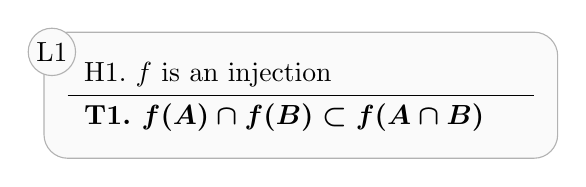
\begin{tikzpicture}[baseline=(main.base)]%
\node[tableau] (main) {%
\\

\begin{tabular}{ll}%
H1.\ $\textrm{$f$ is an injection}$&
\Bstrut\\\hline\Tstrut
\textbf{\boldmath T1.\ $\textrm{$f(A)\cap f(B)\subset f(A\cap B)$}$\unboldmath }&\textbf{\boldmath \unboldmath }
\end{tabular}%
};%
\node[tableaulabel] at (main.north west) [xshift=4mm, yshift=-5.5mm] {L1};
\end{tikzpicture}%
\end{fit}
\smallskip

\noindent1. Expand pre-universal target T1.\nopagebreak[4] 
\marginpar{}\nopagebreak[4] 
\smallskip\nopagebreak[4] 

\begin{fit}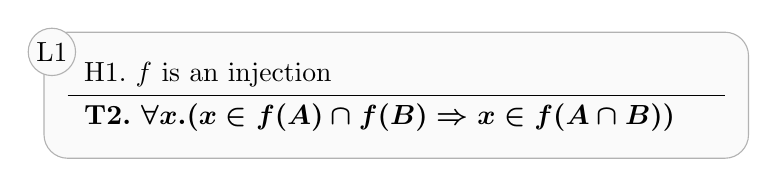
\begin{tikzpicture}[baseline=(main.base)]%
\node[tableau] (main) {%
\\

\begin{tabular}{ll}%
H1.\ $\textrm{$f$ is an injection}$&
\Bstrut\\\hline\Tstrut
\textbf{\boldmath T2.\ $\forall x.(\textrm{$x\in f(A)\cap f(B)$}\Rightarrow \textrm{$x\in f(A\cap B)$})$\unboldmath }&\textbf{\boldmath \unboldmath }
\end{tabular}%
};%
\node[tableaulabel] at (main.north west) [xshift=4mm, yshift=-5.5mm] {L1};
\end{tikzpicture}%
\end{fit}
\smallskip

\noindent2. Apply `let' trick and move premise of universal-conditional target T2 above the line.\nopagebreak[4] 
\marginpar{Let $x$ be an element of $f(A)\cap f(B)$.}\nopagebreak[4] 
\smallskip\nopagebreak[4] 

\begin{fit}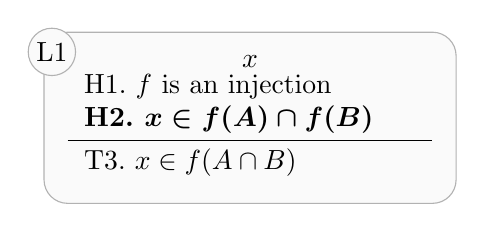
\begin{tikzpicture}[baseline=(main.base)]%
\node[tableau] (main) {%
$x$\\

\begin{tabular}{ll}%
H1.\ $\textrm{$f$ is an injection}$&\\
\textbf{\boldmath H2.\ $\textrm{$x\in f(A)\cap f(B)$}$\unboldmath }&\textbf{\boldmath \unboldmath }
\Bstrut\\\hline\Tstrut
T3.\ $\textrm{$x\in f(A\cap B)$}$&
\end{tabular}%
};%
\node[tableaulabel] at (main.north west) [xshift=4mm, yshift=-5.5mm] {L1};
\end{tikzpicture}%
\end{fit}
\smallskip

\noindent3. Quantifier-free expansion of hypothesis H2.\nopagebreak[4] 
\marginpar{Since $x\in f(A)\cap f(B)$, $x\in f(A)$ and $x\in f(B)$.}\nopagebreak[4] 
\smallskip\nopagebreak[4] 

\begin{fit}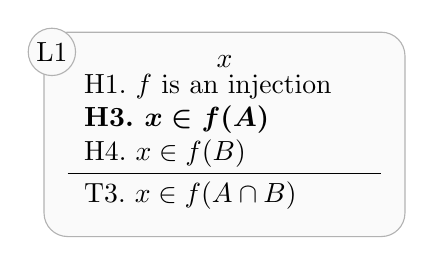
\begin{tikzpicture}[baseline=(main.base)]%
\node[tableau] (main) {%
$x$\\

\begin{tabular}{ll}%
H1.\ $\textrm{$f$ is an injection}$&\\
\textbf{\boldmath H3.\ $\textrm{$x\in f(A)$}$\unboldmath }&\textbf{\boldmath \unboldmath }\\
H4.\ $\textrm{$x\in f(B)$}$&
\Bstrut\\\hline\Tstrut
T3.\ $\textrm{$x\in f(A\cap B)$}$&
\end{tabular}%
};%
\node[tableaulabel] at (main.north west) [xshift=4mm, yshift=-5.5mm] {L1};
\end{tikzpicture}%
\end{fit}
\smallskip

\noindent4. Expand pre-existential hypothesis H3.\nopagebreak[4] 
\marginpar{By definition, since $x\in f(A)$, there exists $y\in A$ such that $f(y) = x$.}\nopagebreak[4] 
\smallskip\nopagebreak[4] 

\begin{fit}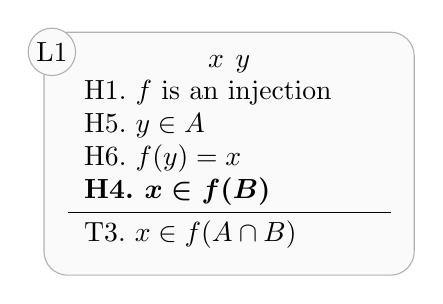
\begin{tikzpicture}[baseline=(main.base)]%
\node[tableau] (main) {%
$x$\hspace{1.5mm}$y$\\

\begin{tabular}{ll}%
H1.\ $\textrm{$f$ is an injection}$&\\
H5.\ $\textrm{$y\in A$}$&\\
H6.\ $\textrm{$f(y) = x$}$&\\
\textbf{\boldmath H4.\ $\textrm{$x\in f(B)$}$\unboldmath }&\textbf{\boldmath \unboldmath }
\Bstrut\\\hline\Tstrut
T3.\ $\textrm{$x\in f(A\cap B)$}$&
\end{tabular}%
};%
\node[tableaulabel] at (main.north west) [xshift=4mm, yshift=-5.5mm] {L1};
\end{tikzpicture}%
\end{fit}
\smallskip

\noindent5. Expand pre-existential hypothesis H4.\nopagebreak[4] 
\marginpar{By definition, since $x\in f(B)$, there exists $z\in B$ such that $f(z) = x$.}\nopagebreak[4] 
\smallskip\nopagebreak[4] 

\begin{fit}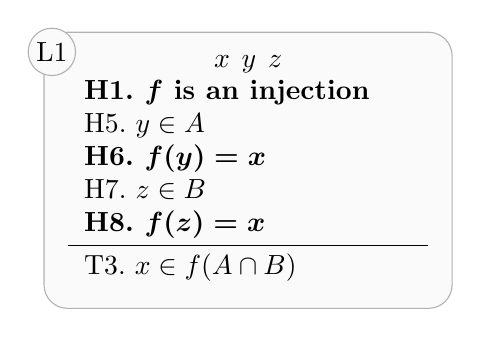
\begin{tikzpicture}[baseline=(main.base)]%
\node[tableau] (main) {%
$x$\hspace{1.5mm}$y$\hspace{1.5mm}$z$\\

\begin{tabular}{ll}%
\textbf{\boldmath H1.\ $\textrm{$f$ is an injection}$\unboldmath }&\textbf{\boldmath \unboldmath }\\
H5.\ $\textrm{$y\in A$}$&\\
\textbf{\boldmath H6.\ $\textrm{$f(y) = x$}$\unboldmath }&\textbf{\boldmath \unboldmath }\\
H7.\ $\textrm{$z\in B$}$&\\
\textbf{\boldmath H8.\ $\textrm{$f(z) = x$}$\unboldmath }&\textbf{\boldmath \unboldmath }
\Bstrut\\\hline\Tstrut
T3.\ $\textrm{$x\in f(A\cap B)$}$&
\end{tabular}%
};%
\node[tableaulabel] at (main.north west) [xshift=4mm, yshift=-5.5mm] {L1};
\end{tikzpicture}%
\end{fit}
\smallskip

\noindent6. Forwards reasoning using H1 with (H6,H8).\nopagebreak[4] 
\marginpar{Since $f$ is an injection, $f(y) = x$ and $f(z) = x$, we have that $y = z$.}\nopagebreak[4] 
\smallskip\nopagebreak[4] 

\begin{fit}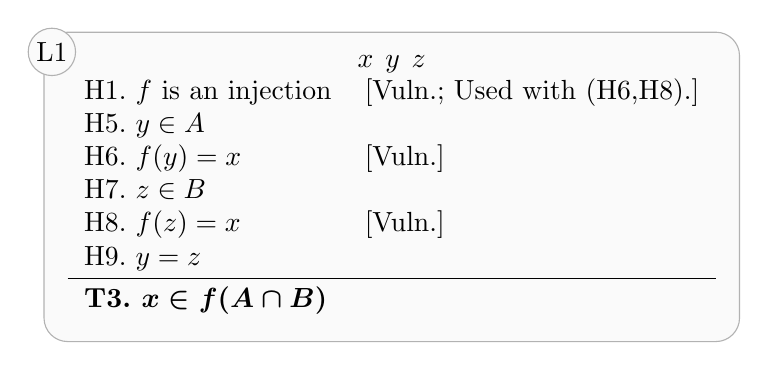
\begin{tikzpicture}[baseline=(main.base)]%
\node[tableau] (main) {%
$x$\hspace{1.5mm}$y$\hspace{1.5mm}$z$\\

\begin{tabular}{ll}%
H1.\ $\textrm{$f$ is an injection}$&[Vuln.; Used with (H6,H8).]\\
H5.\ $\textrm{$y\in A$}$&\\
H6.\ $\textrm{$f(y) = x$}$&[Vuln.]\\
H7.\ $\textrm{$z\in B$}$&\\
H8.\ $\textrm{$f(z) = x$}$&[Vuln.]\\
H9.\ $\textrm{$y = z$}$&
\Bstrut\\\hline\Tstrut
\textbf{\boldmath T3.\ $\textrm{$x\in f(A\cap B)$}$\unboldmath }&\textbf{\boldmath \unboldmath }
\end{tabular}%
};%
\node[tableaulabel] at (main.north west) [xshift=4mm, yshift=-5.5mm] {L1};
\end{tikzpicture}%
\end{fit}
\smallskip

\noindent7. Expand pre-existential target T3.\nopagebreak[4] 
\marginpar{We would like to find $u\in A\cap B$ s.t. $f(u) = x$.}\nopagebreak[4] 
\smallskip\nopagebreak[4] 

\begin{fit}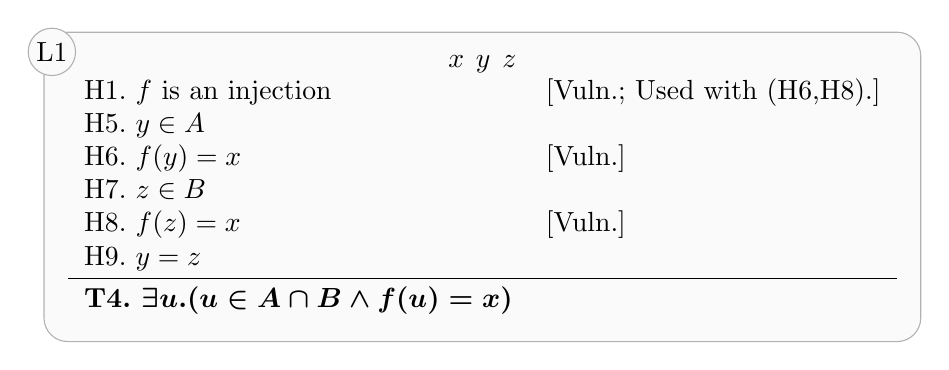
\begin{tikzpicture}[baseline=(main.base)]%
\node[tableau] (main) {%
$x$\hspace{1.5mm}$y$\hspace{1.5mm}$z$\\

\begin{tabular}{ll}%
H1.\ $\textrm{$f$ is an injection}$&[Vuln.; Used with (H6,H8).]\\
H5.\ $\textrm{$y\in A$}$&\\
H6.\ $\textrm{$f(y) = x$}$&[Vuln.]\\
H7.\ $\textrm{$z\in B$}$&\\
H8.\ $\textrm{$f(z) = x$}$&[Vuln.]\\
H9.\ $\textrm{$y = z$}$&
\Bstrut\\\hline\Tstrut
\textbf{\boldmath T4.\ $\exists u.(\textrm{$u\in A\cap B$}\wedge \textrm{$f(u) = x$})$\unboldmath }&\textbf{\boldmath \unboldmath }
\end{tabular}%
};%
\node[tableaulabel] at (main.north west) [xshift=4mm, yshift=-5.5mm] {L1};
\end{tikzpicture}%
\end{fit}
\smallskip

\noindent8. Unlock existential target T4.\nopagebreak[4] 
\marginpar{We would like to find $u\in A\cap B$ s.t. $f(u) = x$.}\nopagebreak[4] 
\smallskip\nopagebreak[4] 

\begin{fit}\begin{tikzpicture}[baseline=(main.base)]%
\node[tableau] (main) {%
$x$\hspace{1.5mm}$y$\hspace{1.5mm}$z$\\

\begin{tabular}{ll}%
H1.\ $\textrm{$f$ is an injection}$&[Vuln.; Used with (H6,H8).]\\
H5.\ $\textrm{$y\in A$}$&\\
H6.\ $\textrm{$f(y) = x$}$&[Vuln.]\\
H7.\ $\textrm{$z\in B$}$&\\
H8.\ $\textrm{$f(z) = x$}$&[Vuln.]\\
H9.\ $\textrm{$y = z$}$&
\Bstrut\\\hline\Tstrut
\begin{tikzpicture}[baseline=(main.base)]%
\node[tableau] (main) {%
$u^\blacklozenge $\\

\begin{tabular}{ll}%

\Bstrut\\\hline\Tstrut
\textbf{\boldmath T5.\ $\textrm{$u^\blacklozenge \in A\cap B$}$\unboldmath }&\textbf{\boldmath \unboldmath }\\
T6.\ $\textrm{$f(u^\blacklozenge ) = x$}$&
\end{tabular}%
};%
\node[tableaulabel] at (main.north west) [xshift=4mm, yshift=-5.5mm] {L2$^\blacklozenge$};
\end{tikzpicture}%

\end{tabular}%
};%
\node[tableaulabel] at (main.north west) [xshift=4mm, yshift=-5.5mm] {L1};
\end{tikzpicture}%
\end{fit}
\smallskip

\noindent9. Quantifier-free expansion of target T5.\nopagebreak[4] 
\marginpar{But $u\in A\cap B$ if and only if $u\in A$ and $u\in B$.}\nopagebreak[4] 
\smallskip\nopagebreak[4] 

\begin{fit}\begin{tikzpicture}[baseline=(main.base)]%
\node[tableau] (main) {%
$x$\hspace{1.5mm}$y$\hspace{1.5mm}$z$\\

\begin{tabular}{ll}%
H1.\ $\textrm{$f$ is an injection}$&[Vuln.; Used with (H6,H8).]\\
H5.\ $\textrm{$y\in A$}$&\\
H6.\ $\textrm{$f(y) = x$}$&[Vuln.]\\
H7.\ $\textrm{$z\in B$}$&\\
H8.\ $\textrm{$f(z) = x$}$&[Vuln.]\\
\textbf{\boldmath H9.\ $\textrm{$y = z$}$\unboldmath }&\textbf{\boldmath \unboldmath }
\Bstrut\\\hline\Tstrut
\begin{tikzpicture}[baseline=(main.base)]%
\node[tableau] (main) {%
$u^\blacklozenge $\\

\begin{tabular}{ll}%

\Bstrut\\\hline\Tstrut
T7.\ $\textrm{$u^\blacklozenge \in A$}$&\\
T8.\ $\textrm{$u^\blacklozenge \in B$}$&\\
T6.\ $\textrm{$f(u^\blacklozenge ) = x$}$&
\end{tabular}%
};%
\node[tableaulabel] at (main.north west) [xshift=4mm, yshift=-5.5mm] {L2$^\blacklozenge$};
\end{tikzpicture}%

\end{tabular}%
};%
\node[tableaulabel] at (main.north west) [xshift=4mm, yshift=-5.5mm] {L1};
\end{tikzpicture}%
\end{fit}
\smallskip

\noindent10. Rewrite $z$ as $y$ throughout the tableau using hypothesis H9.\nopagebreak[4] 
\marginpar{Since $y = z$, we have that $y\in B$.}\nopagebreak[4] 
\smallskip\nopagebreak[4] 

\begin{fit}\begin{tikzpicture}[baseline=(main.base)]%
\node[tableau] (main) {%
$x$\hspace{1.5mm}$y$\hspace{1.5mm}$z$\\

\begin{tabular}{ll}%
H1.\ $\textrm{$f$ is an injection}$&[Vuln.; Used with (H6,H8).]\\
H5.\ $\textrm{$y\in A$}$&\\
H6.\ $\textrm{$f(y) = x$}$&[Vuln.]\\
H10.\ $\textrm{$y\in B$}$&
\Bstrut\\\hline\Tstrut
\begin{tikzpicture}[baseline=(main.base)]%
\node[tableau] (main) {%
$u^\blacklozenge $\\

\begin{tabular}{ll}%

\Bstrut\\\hline\Tstrut
T7.\ $\textrm{$u^\blacklozenge \in A$}$&\\
T8.\ $\textrm{$u^\blacklozenge \in B$}$&\\
T6.\ $\textrm{$f(u^\blacklozenge ) = x$}$&
\end{tabular}%
};%
\node[tableaulabel] at (main.north west) [xshift=4mm, yshift=-5.5mm] {L2$^\blacklozenge$};
\end{tikzpicture}%

\end{tabular}%
};%
\node[tableaulabel] at (main.north west) [xshift=4mm, yshift=-5.5mm] {L1};
\end{tikzpicture}%
\end{fit}
\smallskip

\noindent11. Moved H6 down, as $x$ can only be utilised by T6.\nopagebreak[4] 
\marginpar{}\nopagebreak[4] 
\smallskip\nopagebreak[4] 

\begin{fit}\begin{tikzpicture}[baseline=(main.base)]%
\node[tableau] (main) {%
$x$\hspace{1.5mm}$y$\hspace{1.5mm}$z$\\

\begin{tabular}{ll}%
H1.\ $\textrm{$f$ is an injection}$&[Vuln.; Used with (H6,H8).]\\
H5.\ $\textrm{$y\in A$}$&\\
H10.\ $\textrm{$y\in B$}$&
\Bstrut\\\hline\Tstrut
\begin{tikzpicture}[baseline=(main.base)]%
\node[tableau] (main) {%
$u^\blacklozenge $\\

\begin{tabular}{ll}%

\Bstrut\\\hline\Tstrut
T7.\ $\textrm{$u^\blacklozenge \in A$}$&\\
T8.\ $\textrm{$u^\blacklozenge \in B$}$&\\
\begin{tikzpicture}[baseline=(main.base)]%
\node[tableau] (main) {%
\\

\begin{tabular}{ll}%
H6.\ $\textrm{$f(y) = x$}$&[Vuln.; From L1.]
\Bstrut\\\hline\Tstrut
T6.\ $\textrm{$f(u^\blacklozenge ) = x$}$&
\end{tabular}%
};%
\node[tableaulabel] at (main.north west) [xshift=4mm, yshift=-5.5mm] {L3};
\end{tikzpicture}%

\end{tabular}%
};%
\node[tableaulabel] at (main.north west) [xshift=4mm, yshift=-5.5mm] {L2$^\blacklozenge$};
\end{tikzpicture}%

\end{tabular}%
};%
\node[tableaulabel] at (main.north west) [xshift=4mm, yshift=-5.5mm] {L1};
\end{tikzpicture}%
\end{fit}
\smallskip

\noindent12. Choosing $u^\blacklozenge  = y$ matches all targets inside L2$^\blacklozenge$ against hypotheses, so L2$^\blacklozenge$ is done.\nopagebreak[4] 
\marginpar{Therefore, setting $u = y$, we are done.}\nopagebreak[4] 
\smallskip\nopagebreak[4] 

\begin{fit}\begin{tikzpicture}[baseline=(main.base)]%
\node[tableau] (main) {%
$x$\hspace{1.5mm}$y$\hspace{1.5mm}$z$\\

\begin{tabular}{ll}%
H1.\ $\textrm{$f$ is an injection}$&[Vuln.; Used with (H6,H8).]\\
H5.\ $\textrm{$y\in A$}$&\\
H10.\ $\textrm{$y\in B$}$&
\Bstrut\\\hline\Tstrut
\begin{tikzpicture}%
\node[tableau] (main) {%
\ \ \,Done
};%
\node[tableaulabel] at (main.north west) [xshift=4mm, yshift=-5.5mm] {L2$^\blacklozenge$};
\end{tikzpicture}%

\end{tabular}%
};%
\node[tableaulabel] at (main.north west) [xshift=4mm, yshift=-5.5mm] {L1};
\end{tikzpicture}%
\end{fit}
\smallskip

\noindent13. All targets of L1 are `Done', so L1 is itself done.\nopagebreak[4] 
\marginpar{}\nopagebreak[4] 
\smallskip\nopagebreak[4] 

\begin{fit}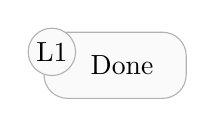
\begin{tikzpicture}%
\node[tableau] (main) {%
\ \ \,Done
};%
\node[tableaulabel] at (main.north west) [xshift=4mm, yshift=-5.5mm] {L1};
\end{tikzpicture}%
\end{fit}

Problem solved.
\cleardoublepage

\end{steps}
{\begin{center} \large \textbf{If $g,f$ are injections then $(g \circ f)$ is an injection.}\end{center}}\nopagebreak[4]

\begin{center}
\begin{minipage}{120mm}
Let $x$, $y$ and $z$ be such that $g(f(x)) = z$ and $g(f(y)) = z$. Then, since $g$ is an injection, we have that $f(x) = f(y)$. Therefore, since $f$ is an injection, $x = y$ if $f(y) = f(y)$. Since $g$ is an injection and $g(f(y)) = z$, $f(y) = f(y)$ if $g(f(y)) = z$. But this is clearly the case, so we are done.
\end{minipage}
\end{center}

\bigskip
\begin{steps}
\begin{fit}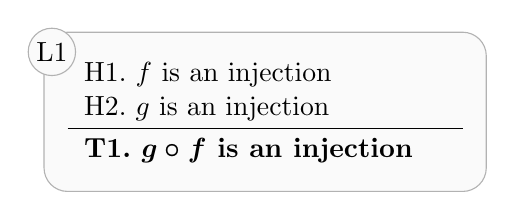
\begin{tikzpicture}[baseline=(main.base)]%
\node[tableau] (main) {%
\\

\begin{tabular}{ll}%
H1.\ $\textrm{$f$ is an injection}$&\\
H2.\ $\textrm{$g$ is an injection}$&
\Bstrut\\\hline\Tstrut
\textbf{\boldmath T1.\ $\textrm{$g\circ f$ is an injection}$\unboldmath }&\textbf{\boldmath \unboldmath }
\end{tabular}%
};%
\node[tableaulabel] at (main.north west) [xshift=4mm, yshift=-5.5mm] {L1};
\end{tikzpicture}%
\end{fit}
\smallskip

\noindent1. Expand pre-universal target T1.\nopagebreak[4] 
\marginpar{}\nopagebreak[4] 
\smallskip\nopagebreak[4] 

\begin{fit}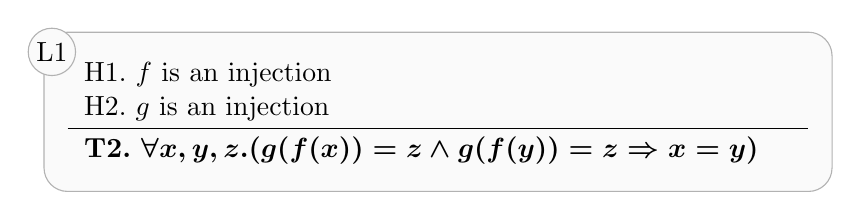
\begin{tikzpicture}[baseline=(main.base)]%
\node[tableau] (main) {%
\\

\begin{tabular}{ll}%
H1.\ $\textrm{$f$ is an injection}$&\\
H2.\ $\textrm{$g$ is an injection}$&
\Bstrut\\\hline\Tstrut
\textbf{\boldmath T2.\ $\forall x, y, z.(\textrm{$g(f(x)) = z$}\wedge \textrm{$g(f(y)) = z$}\Rightarrow \textrm{$x = y$})$\unboldmath }&\textbf{\boldmath \unboldmath }
\end{tabular}%
};%
\node[tableaulabel] at (main.north west) [xshift=4mm, yshift=-5.5mm] {L1};
\end{tikzpicture}%
\end{fit}
\smallskip

\noindent2. Apply `let' trick and move premise of universal-conditional target T2 above the line.\nopagebreak[4] 
\marginpar{Let $x$, $y$ and $z$ be such that $g(f(x)) = z$ and $g(f(y)) = z$.}\nopagebreak[4] 
\smallskip\nopagebreak[4] 

\begin{fit}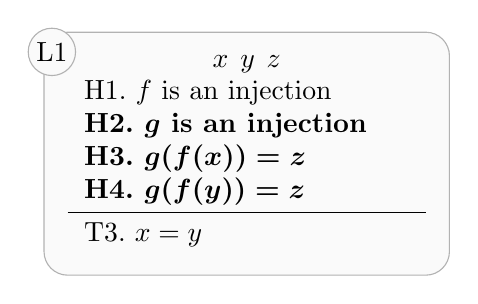
\begin{tikzpicture}[baseline=(main.base)]%
\node[tableau] (main) {%
$x$\hspace{1.5mm}$y$\hspace{1.5mm}$z$\\

\begin{tabular}{ll}%
H1.\ $\textrm{$f$ is an injection}$&\\
\textbf{\boldmath H2.\ $\textrm{$g$ is an injection}$\unboldmath }&\textbf{\boldmath \unboldmath }\\
\textbf{\boldmath H3.\ $\textrm{$g(f(x)) = z$}$\unboldmath }&\textbf{\boldmath \unboldmath }\\
\textbf{\boldmath H4.\ $\textrm{$g(f(y)) = z$}$\unboldmath }&\textbf{\boldmath \unboldmath }
\Bstrut\\\hline\Tstrut
T3.\ $\textrm{$x = y$}$&
\end{tabular}%
};%
\node[tableaulabel] at (main.north west) [xshift=4mm, yshift=-5.5mm] {L1};
\end{tikzpicture}%
\end{fit}
\smallskip

\noindent3. Forwards reasoning using H2 with (H3,H4).\nopagebreak[4] 
\marginpar{Since $g$ is an injection, $g(f(x)) = z$ and $g(f(y)) = z$, we have that $f(x) = f(y)$.}\nopagebreak[4] 
\smallskip\nopagebreak[4] 

\begin{fit}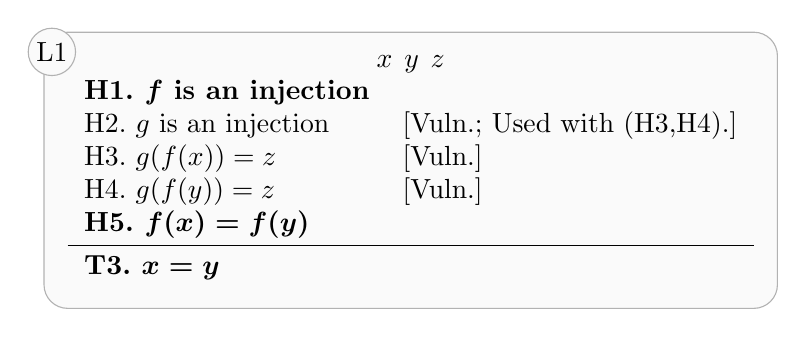
\begin{tikzpicture}[baseline=(main.base)]%
\node[tableau] (main) {%
$x$\hspace{1.5mm}$y$\hspace{1.5mm}$z$\\

\begin{tabular}{ll}%
\textbf{\boldmath H1.\ $\textrm{$f$ is an injection}$\unboldmath }&\textbf{\boldmath \unboldmath }\\
H2.\ $\textrm{$g$ is an injection}$&[Vuln.; Used with (H3,H4).]\\
H3.\ $\textrm{$g(f(x)) = z$}$&[Vuln.]\\
H4.\ $\textrm{$g(f(y)) = z$}$&[Vuln.]\\
\textbf{\boldmath H5.\ $\textrm{$f(x) = f(y)$}$\unboldmath }&\textbf{\boldmath \unboldmath }
\Bstrut\\\hline\Tstrut
\textbf{\boldmath T3.\ $\textrm{$x = y$}$\unboldmath }&\textbf{\boldmath \unboldmath }
\end{tabular}%
};%
\node[tableaulabel] at (main.north west) [xshift=4mm, yshift=-5.5mm] {L1};
\end{tikzpicture}%
\end{fit}
\smallskip

\noindent4. Backwards reasoning using H1 with (T3,H5).\nopagebreak[4] 
\marginpar{Since $f$ is an injection and $f(x) = f(y)$, $x = y$ if $f(y) = f(y)$.}\nopagebreak[4] 
\smallskip\nopagebreak[4] 

\begin{fit}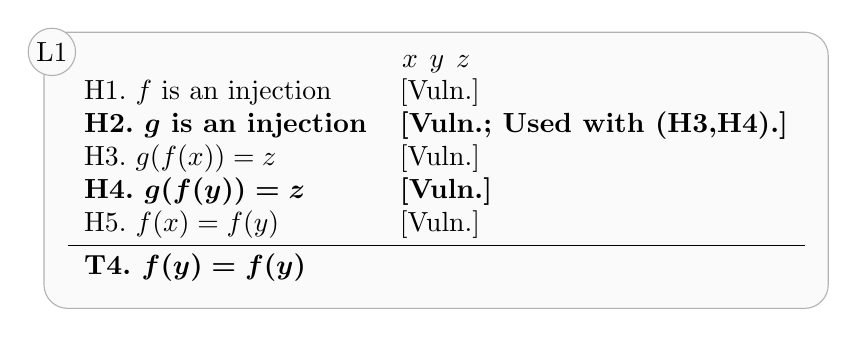
\begin{tikzpicture}[baseline=(main.base)]%
\node[tableau] (main) {%
$x$\hspace{1.5mm}$y$\hspace{1.5mm}$z$\\

\begin{tabular}{ll}%
H1.\ $\textrm{$f$ is an injection}$&[Vuln.]\\
\textbf{\boldmath H2.\ $\textrm{$g$ is an injection}$\unboldmath }&\textbf{\boldmath [Vuln.; Used with (H3,H4).]\unboldmath }\\
H3.\ $\textrm{$g(f(x)) = z$}$&[Vuln.]\\
\textbf{\boldmath H4.\ $\textrm{$g(f(y)) = z$}$\unboldmath }&\textbf{\boldmath [Vuln.]\unboldmath }\\
H5.\ $\textrm{$f(x) = f(y)$}$&[Vuln.]
\Bstrut\\\hline\Tstrut
\textbf{\boldmath T4.\ $\textrm{$f(y) = f(y)$}$\unboldmath }&\textbf{\boldmath \unboldmath }
\end{tabular}%
};%
\node[tableaulabel] at (main.north west) [xshift=4mm, yshift=-5.5mm] {L1};
\end{tikzpicture}%
\end{fit}
\smallskip

\noindent5. Backwards reasoning using H2 with (T4,H4).\nopagebreak[4] 
\marginpar{Since $g$ is an injection and $g(f(y)) = z$, $f(y) = f(y)$ if $g(f(y)) = z$.}\nopagebreak[4] 
\smallskip\nopagebreak[4] 

\begin{fit}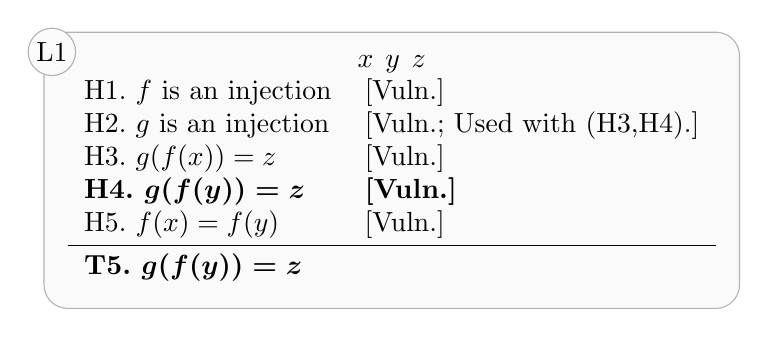
\begin{tikzpicture}[baseline=(main.base)]%
\node[tableau] (main) {%
$x$\hspace{1.5mm}$y$\hspace{1.5mm}$z$\\

\begin{tabular}{ll}%
H1.\ $\textrm{$f$ is an injection}$&[Vuln.]\\
H2.\ $\textrm{$g$ is an injection}$&[Vuln.; Used with (H3,H4).]\\
H3.\ $\textrm{$g(f(x)) = z$}$&[Vuln.]\\
\textbf{\boldmath H4.\ $\textrm{$g(f(y)) = z$}$\unboldmath }&\textbf{\boldmath [Vuln.]\unboldmath }\\
H5.\ $\textrm{$f(x) = f(y)$}$&[Vuln.]
\Bstrut\\\hline\Tstrut
\textbf{\boldmath T5.\ $\textrm{$g(f(y)) = z$}$\unboldmath }&\textbf{\boldmath \unboldmath }
\end{tabular}%
};%
\node[tableaulabel] at (main.north west) [xshift=4mm, yshift=-5.5mm] {L1};
\end{tikzpicture}%
\end{fit}
\smallskip

\noindent6. Hypothesis H4 matches target T5, so L1 is done.\nopagebreak[4] 
\marginpar{But this is clearly the case, so we are done.}\nopagebreak[4] 
\smallskip\nopagebreak[4] 

\begin{fit}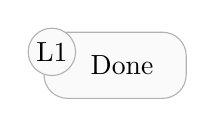
\begin{tikzpicture}%
\node[tableau] (main) {%
\ \ \,Done
};%
\node[tableaulabel] at (main.north west) [xshift=4mm, yshift=-5.5mm] {L1};
\end{tikzpicture}%
\end{fit}

Problem solved.
\cleardoublepage

\end{steps}
{\begin{center} \large \textbf{Prove that $A \subseteq f^{-1}(f(A))$}\end{center}}\nopagebreak[4]

\begin{center}
\begin{minipage}{120mm}
Let $x$ be an element of $A$. We would like to show that $x\in f^{-1}(f(A))$, i.e. that $f(x)\in f(A)$. But this is clearly the case, so we are done.
\end{minipage}
\end{center}

\bigskip
\begin{steps}
\begin{fit}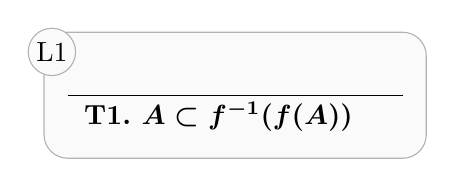
\begin{tikzpicture}[baseline=(main.base)]%
\node[tableau] (main) {%
\\

\begin{tabular}{ll}%

\Bstrut\\\hline\Tstrut
\textbf{\boldmath T1.\ $\textrm{$A\subset f^{-1}(f(A))$}$\unboldmath }&\textbf{\boldmath \unboldmath }
\end{tabular}%
};%
\node[tableaulabel] at (main.north west) [xshift=4mm, yshift=-5.5mm] {L1};
\end{tikzpicture}%
\end{fit}
\smallskip

\noindent1. Expand pre-universal target T1.\nopagebreak[4] 
\marginpar{}\nopagebreak[4] 
\smallskip\nopagebreak[4] 

\begin{fit}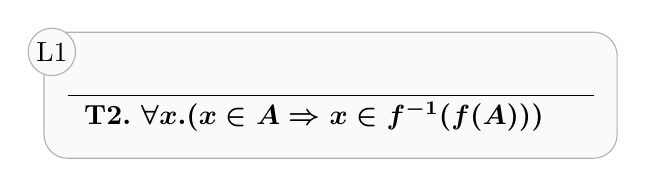
\begin{tikzpicture}[baseline=(main.base)]%
\node[tableau] (main) {%
\\

\begin{tabular}{ll}%

\Bstrut\\\hline\Tstrut
\textbf{\boldmath T2.\ $\forall x.(\textrm{$x\in A$}\Rightarrow \textrm{$x\in f^{-1}(f(A))$})$\unboldmath }&\textbf{\boldmath \unboldmath }
\end{tabular}%
};%
\node[tableaulabel] at (main.north west) [xshift=4mm, yshift=-5.5mm] {L1};
\end{tikzpicture}%
\end{fit}
\smallskip

\noindent2. Apply `let' trick and move premise of universal-conditional target T2 above the line.\nopagebreak[4] 
\marginpar{Let $x$ be an element of $A$.}\nopagebreak[4] 
\smallskip\nopagebreak[4] 

\begin{fit}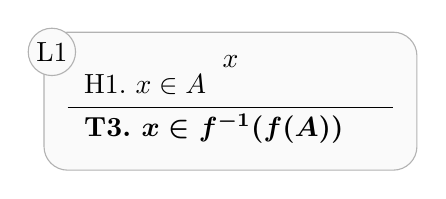
\begin{tikzpicture}[baseline=(main.base)]%
\node[tableau] (main) {%
$x$\\

\begin{tabular}{ll}%
H1.\ $\textrm{$x\in A$}$&
\Bstrut\\\hline\Tstrut
\textbf{\boldmath T3.\ $\textrm{$x\in f^{-1}(f(A))$}$\unboldmath }&\textbf{\boldmath \unboldmath }
\end{tabular}%
};%
\node[tableaulabel] at (main.north west) [xshift=4mm, yshift=-5.5mm] {L1};
\end{tikzpicture}%
\end{fit}
\smallskip

\noindent3. Quantifier-free expansion of target T3.\nopagebreak[4] 
\marginpar{We would like to show that $x\in f^{-1}(f(A))$, i.e. that $f(x)\in f(A)$.}\nopagebreak[4] 
\smallskip\nopagebreak[4] 

\begin{fit}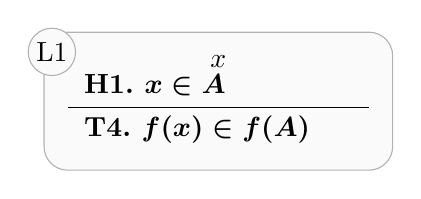
\begin{tikzpicture}[baseline=(main.base)]%
\node[tableau] (main) {%
$x$\\

\begin{tabular}{ll}%
\textbf{\boldmath H1.\ $\textrm{$x\in A$}$\unboldmath }&\textbf{\boldmath \unboldmath }
\Bstrut\\\hline\Tstrut
\textbf{\boldmath T4.\ $\textrm{$f(x)\in f(A)$}$\unboldmath }&\textbf{\boldmath \unboldmath }
\end{tabular}%
};%
\node[tableaulabel] at (main.north west) [xshift=4mm, yshift=-5.5mm] {L1};
\end{tikzpicture}%
\end{fit}
\smallskip

\noindent4. All conjuncts of T4 (after expansion) can be simultaneously matched against H1 or rendered trivial by choosing $y = x$, so L1 is done.\nopagebreak[4] 
\marginpar{We would like to show that $f(x)\in f(A)$. But this is clearly the case, so we are done.}\nopagebreak[4] 
\smallskip\nopagebreak[4] 

\begin{fit}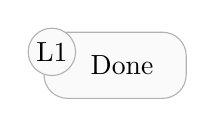
\begin{tikzpicture}%
\node[tableau] (main) {%
\ \ \,Done
};%
\node[tableaulabel] at (main.north west) [xshift=4mm, yshift=-5.5mm] {L1};
\end{tikzpicture}%
\end{fit}

Problem solved.
\cleardoublepage

\end{steps}
{\begin{center} \large \textbf{Prove that $f(f^{-1}(A))\subset A$}\end{center}}\nopagebreak[4]

\begin{center}
\begin{minipage}{120mm}
Let $x$ be an element of $f(f^{-1}(A))$. Then there exists $y\in f^{-1}(A)$ such that $f(y) = x$. Since $y\in f^{-1}(A)$, we have that $f(y)\in A$. Since $f(y) = x$, we have that $x\in A$. But this is clearly the case, so we are done.
\end{minipage}
\end{center}

\bigskip
\begin{steps}
\begin{fit}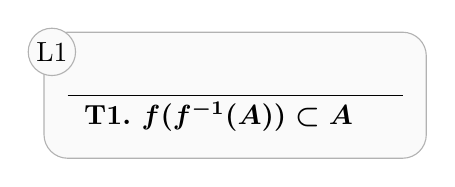
\begin{tikzpicture}[baseline=(main.base)]%
\node[tableau] (main) {%
\\

\begin{tabular}{ll}%

\Bstrut\\\hline\Tstrut
\textbf{\boldmath T1.\ $\textrm{$f(f^{-1}(A))\subset A$}$\unboldmath }&\textbf{\boldmath \unboldmath }
\end{tabular}%
};%
\node[tableaulabel] at (main.north west) [xshift=4mm, yshift=-5.5mm] {L1};
\end{tikzpicture}%
\end{fit}
\smallskip

\noindent1. Expand pre-universal target T1.\nopagebreak[4] 
\marginpar{}\nopagebreak[4] 
\smallskip\nopagebreak[4] 

\begin{fit}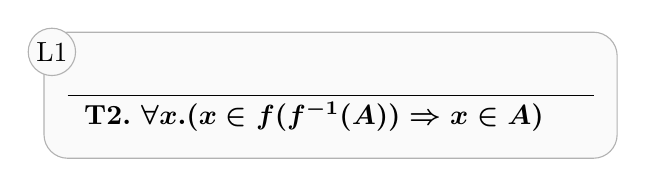
\begin{tikzpicture}[baseline=(main.base)]%
\node[tableau] (main) {%
\\

\begin{tabular}{ll}%

\Bstrut\\\hline\Tstrut
\textbf{\boldmath T2.\ $\forall x.(\textrm{$x\in f(f^{-1}(A))$}\Rightarrow \textrm{$x\in A$})$\unboldmath }&\textbf{\boldmath \unboldmath }
\end{tabular}%
};%
\node[tableaulabel] at (main.north west) [xshift=4mm, yshift=-5.5mm] {L1};
\end{tikzpicture}%
\end{fit}
\smallskip

\noindent2. Apply `let' trick and move premise of universal-conditional target T2 above the line.\nopagebreak[4] 
\marginpar{Let $x$ be an element of $f(f^{-1}(A))$.}\nopagebreak[4] 
\smallskip\nopagebreak[4] 

\begin{fit}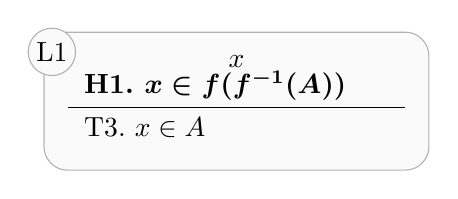
\begin{tikzpicture}[baseline=(main.base)]%
\node[tableau] (main) {%
$x$\\

\begin{tabular}{ll}%
\textbf{\boldmath H1.\ $\textrm{$x\in f(f^{-1}(A))$}$\unboldmath }&\textbf{\boldmath \unboldmath }
\Bstrut\\\hline\Tstrut
T3.\ $\textrm{$x\in A$}$&
\end{tabular}%
};%
\node[tableaulabel] at (main.north west) [xshift=4mm, yshift=-5.5mm] {L1};
\end{tikzpicture}%
\end{fit}
\smallskip

\noindent3. Expand pre-existential hypothesis H1.\nopagebreak[4] 
\marginpar{By definition, since $x\in f(f^{-1}(A))$, there exists $y\in f^{-1}(A)$ such that $f(y) = x$.}\nopagebreak[4] 
\smallskip\nopagebreak[4] 

\begin{fit}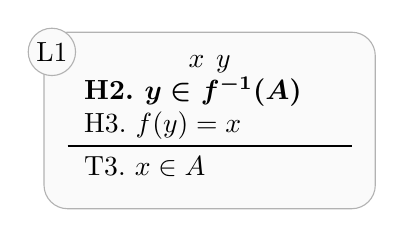
\begin{tikzpicture}[baseline=(main.base)]%
\node[tableau] (main) {%
$x$\hspace{1.5mm}$y$\\

\begin{tabular}{ll}%
\textbf{\boldmath H2.\ $\textrm{$y\in f^{-1}(A)$}$\unboldmath }&\textbf{\boldmath \unboldmath }\\
H3.\ $\textrm{$f(y) = x$}$&
\Bstrut\\\hline\Tstrut
T3.\ $\textrm{$x\in A$}$&
\end{tabular}%
};%
\node[tableaulabel] at (main.north west) [xshift=4mm, yshift=-5.5mm] {L1};
\end{tikzpicture}%
\end{fit}
\smallskip

\noindent4. Quantifier-free expansion of hypothesis H2.\nopagebreak[4] 
\marginpar{Since $y\in f^{-1}(A)$, we have that $f(y)\in A$.}\nopagebreak[4] 
\smallskip\nopagebreak[4] 

\begin{fit}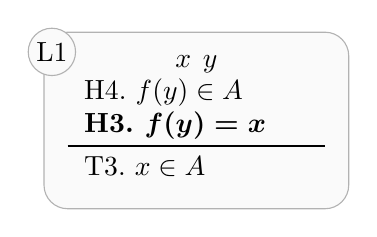
\begin{tikzpicture}[baseline=(main.base)]%
\node[tableau] (main) {%
$x$\hspace{1.5mm}$y$\\

\begin{tabular}{ll}%
H4.\ $\textrm{$f(y)\in A$}$&\\
\textbf{\boldmath H3.\ $\textrm{$f(y) = x$}$\unboldmath }&\textbf{\boldmath \unboldmath }
\Bstrut\\\hline\Tstrut
T3.\ $\textrm{$x\in A$}$&
\end{tabular}%
};%
\node[tableaulabel] at (main.north west) [xshift=4mm, yshift=-5.5mm] {L1};
\end{tikzpicture}%
\end{fit}
\smallskip

\noindent5. Rewrite $f(y)$ as $x$ throughout the tableau using hypothesis H3.\nopagebreak[4] 
\marginpar{Since $f(y) = x$, we have that $x\in A$.}\nopagebreak[4] 
\smallskip\nopagebreak[4] 

\begin{fit}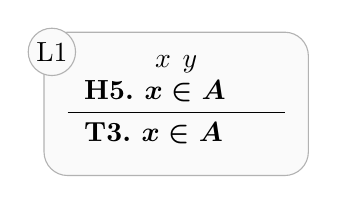
\begin{tikzpicture}[baseline=(main.base)]%
\node[tableau] (main) {%
$x$\hspace{1.5mm}$y$\\

\begin{tabular}{ll}%
\textbf{\boldmath H5.\ $\textrm{$x\in A$}$\unboldmath }&\textbf{\boldmath \unboldmath }
\Bstrut\\\hline\Tstrut
\textbf{\boldmath T3.\ $\textrm{$x\in A$}$\unboldmath }&\textbf{\boldmath \unboldmath }
\end{tabular}%
};%
\node[tableaulabel] at (main.north west) [xshift=4mm, yshift=-5.5mm] {L1};
\end{tikzpicture}%
\end{fit}
\smallskip

\noindent6. Hypothesis H5 matches target T3, so L1 is done.\nopagebreak[4] 
\marginpar{But this is clearly the case, so we are done.}\nopagebreak[4] 
\smallskip\nopagebreak[4] 

\begin{fit}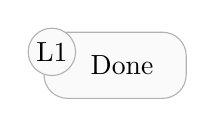
\begin{tikzpicture}%
\node[tableau] (main) {%
\ \ \,Done
};%
\node[tableaulabel] at (main.north west) [xshift=4mm, yshift=-5.5mm] {L1};
\end{tikzpicture}%
\end{fit}

Problem solved.
\cleardoublepage

\end{steps}
{\begin{center} \large \textbf{Prove that $f(A \cap B) \subseteq f(A) \cap f(B)$}\end{center}}\nopagebreak[4]

\begin{center}
\begin{minipage}{120mm}
By definition, since $y\in f(A\cap B)$, there exists $z\in A\cap B$ such that $f(z) = y$. Since $z\in A\cap B$, $z\in A$ and $z\in B$. We would like to show that $y\in f(A)\cap f(B)$, i.e. that $y\in f(A)$ and $y\in f(B)$. We would like to show that $y\in f(A)$. But this is clearly the case, so we are done. Thus $y\in f(B)$ and we are done.
\end{minipage}
\end{center}

\bigskip
\begin{steps}
\begin{fit}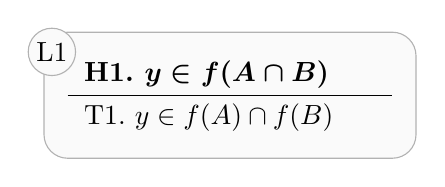
\begin{tikzpicture}[baseline=(main.base)]%
\node[tableau] (main) {%
\\

\begin{tabular}{ll}%
\textbf{\boldmath H1.\ $\textrm{$y\in f(A\cap B)$}$\unboldmath }&\textbf{\boldmath \unboldmath }
\Bstrut\\\hline\Tstrut
T1.\ $\textrm{$y\in f(A)\cap f(B)$}$&
\end{tabular}%
};%
\node[tableaulabel] at (main.north west) [xshift=4mm, yshift=-5.5mm] {L1};
\end{tikzpicture}%
\end{fit}
\smallskip

\noindent1. Expand pre-existential hypothesis H1.\nopagebreak[4] 
\marginpar{By definition, since $y\in f(A\cap B)$, there exists $z\in A\cap B$ such that $f(z) = y$.}\nopagebreak[4] 
\smallskip\nopagebreak[4] 

\begin{fit}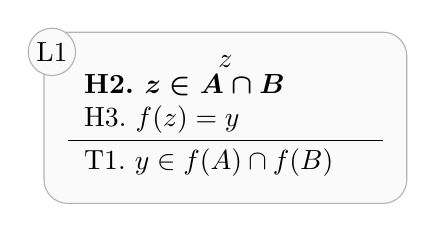
\begin{tikzpicture}[baseline=(main.base)]%
\node[tableau] (main) {%
$z$\\

\begin{tabular}{ll}%
\textbf{\boldmath H2.\ $\textrm{$z\in A\cap B$}$\unboldmath }&\textbf{\boldmath \unboldmath }\\
H3.\ $\textrm{$f(z) = y$}$&
\Bstrut\\\hline\Tstrut
T1.\ $\textrm{$y\in f(A)\cap f(B)$}$&
\end{tabular}%
};%
\node[tableaulabel] at (main.north west) [xshift=4mm, yshift=-5.5mm] {L1};
\end{tikzpicture}%
\end{fit}
\smallskip

\noindent2. Quantifier-free expansion of hypothesis H2.\nopagebreak[4] 
\marginpar{Since $z\in A\cap B$, $z\in A$ and $z\in B$.}\nopagebreak[4] 
\smallskip\nopagebreak[4] 

\begin{fit}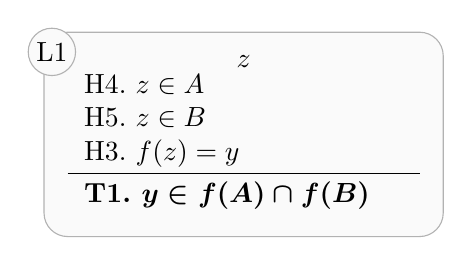
\begin{tikzpicture}[baseline=(main.base)]%
\node[tableau] (main) {%
$z$\\

\begin{tabular}{ll}%
H4.\ $\textrm{$z\in A$}$&\\
H5.\ $\textrm{$z\in B$}$&\\
H3.\ $\textrm{$f(z) = y$}$&
\Bstrut\\\hline\Tstrut
\textbf{\boldmath T1.\ $\textrm{$y\in f(A)\cap f(B)$}$\unboldmath }&\textbf{\boldmath \unboldmath }
\end{tabular}%
};%
\node[tableaulabel] at (main.north west) [xshift=4mm, yshift=-5.5mm] {L1};
\end{tikzpicture}%
\end{fit}
\smallskip

\noindent3. Quantifier-free expansion of target T1.\nopagebreak[4] 
\marginpar{We would like to show that $y\in f(A)\cap f(B)$, i.e. that $y\in f(A)$ and $y\in f(B)$.}\nopagebreak[4] 
\smallskip\nopagebreak[4] 

\begin{fit}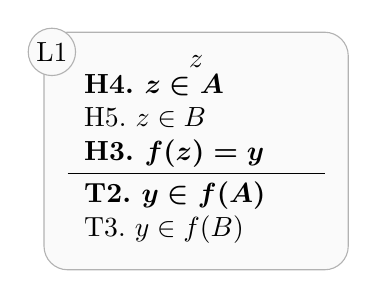
\begin{tikzpicture}[baseline=(main.base)]%
\node[tableau] (main) {%
$z$\\

\begin{tabular}{ll}%
\textbf{\boldmath H4.\ $\textrm{$z\in A$}$\unboldmath }&\textbf{\boldmath \unboldmath }\\
H5.\ $\textrm{$z\in B$}$&\\
\textbf{\boldmath H3.\ $\textrm{$f(z) = y$}$\unboldmath }&\textbf{\boldmath \unboldmath }
\Bstrut\\\hline\Tstrut
\textbf{\boldmath T2.\ $\textrm{$y\in f(A)$}$\unboldmath }&\textbf{\boldmath \unboldmath }\\
T3.\ $\textrm{$y\in f(B)$}$&
\end{tabular}%
};%
\node[tableaulabel] at (main.north west) [xshift=4mm, yshift=-5.5mm] {L1};
\end{tikzpicture}%
\end{fit}
\smallskip

\noindent4. All conjuncts of T2 (after expansion) can be simultaneously matched against H4 and H3 or rendered trivial by choosing $u = z$, so we can remove T2.\nopagebreak[4] 
\marginpar{We would like to show that $y\in f(A)$. But this is clearly the case, so we are done.}\nopagebreak[4] 
\smallskip\nopagebreak[4] 

\begin{fit}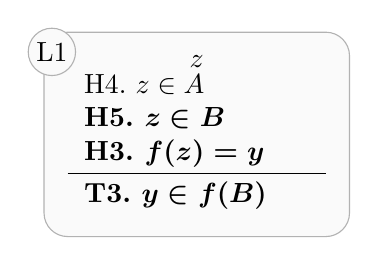
\begin{tikzpicture}[baseline=(main.base)]%
\node[tableau] (main) {%
$z$\\

\begin{tabular}{ll}%
H4.\ $\textrm{$z\in A$}$&\\
\textbf{\boldmath H5.\ $\textrm{$z\in B$}$\unboldmath }&\textbf{\boldmath \unboldmath }\\
\textbf{\boldmath H3.\ $\textrm{$f(z) = y$}$\unboldmath }&\textbf{\boldmath \unboldmath }
\Bstrut\\\hline\Tstrut
\textbf{\boldmath T3.\ $\textrm{$y\in f(B)$}$\unboldmath }&\textbf{\boldmath \unboldmath }
\end{tabular}%
};%
\node[tableaulabel] at (main.north west) [xshift=4mm, yshift=-5.5mm] {L1};
\end{tikzpicture}%
\end{fit}
\smallskip

\noindent5. All conjuncts of T3 (after expansion) can be simultaneously matched against H5 and H3 or rendered trivial by choosing $u = z$, so L1 is done.\nopagebreak[4] 
\marginpar{We would like to show that $y\in f(B)$. But this is clearly the case, so we are done.}\nopagebreak[4] 
\smallskip\nopagebreak[4] 

\begin{fit}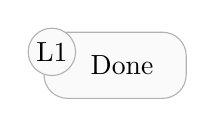
\begin{tikzpicture}%
\node[tableau] (main) {%
\ \ \,Done
};%
\node[tableaulabel] at (main.north west) [xshift=4mm, yshift=-5.5mm] {L1};
\end{tikzpicture}%
\end{fit}

Problem solved.
\cleardoublepage

\end{steps}
{\begin{center} \large \textbf{Prove that $f^{-1}(A \cap B) \subseteq f^{-1}(A) \cap f^{-1}(B)$}\end{center}}\nopagebreak[4]

\begin{center}
\begin{minipage}{120mm}
Since $x\in f^{-1}(A\cap B)$, we have that $f(x)\in A\cap B$. Then $f(x)\in A$ and $f(x)\in B$. We would like to show that $x\in f^{-1}(A)\cap f^{-1}(B)$, i.e. that $x\in f^{-1}(A)$ and $x\in f^{-1}(B)$. We would like to show that $x\in f^{-1}(A)$, i.e. that $f(x)\in A$. We would like to show that $x\in f^{-1}(B)$, i.e. that $f(x)\in B$. But this is clearly the case, so we are done.
\end{minipage}
\end{center}

\bigskip
\begin{steps}
\begin{fit}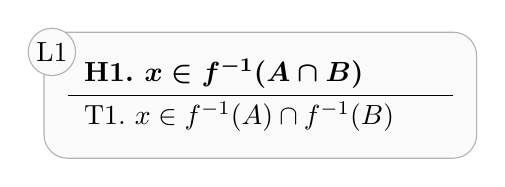
\begin{tikzpicture}[baseline=(main.base)]%
\node[tableau] (main) {%
\\

\begin{tabular}{ll}%
\textbf{\boldmath H1.\ $\textrm{$x\in f^{-1}(A\cap B)$}$\unboldmath }&\textbf{\boldmath \unboldmath }
\Bstrut\\\hline\Tstrut
T1.\ $\textrm{$x\in f^{-1}(A)\cap f^{-1}(B)$}$&
\end{tabular}%
};%
\node[tableaulabel] at (main.north west) [xshift=4mm, yshift=-5.5mm] {L1};
\end{tikzpicture}%
\end{fit}
\smallskip

\noindent1. Quantifier-free expansion of hypothesis H1.\nopagebreak[4] 
\marginpar{Since $x\in f^{-1}(A\cap B)$, we have that $f(x)\in A\cap B$.}\nopagebreak[4] 
\smallskip\nopagebreak[4] 

\begin{fit}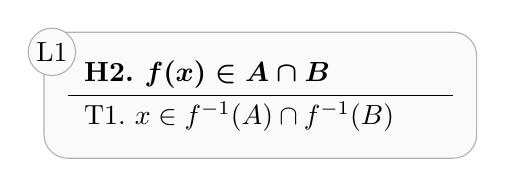
\begin{tikzpicture}[baseline=(main.base)]%
\node[tableau] (main) {%
\\

\begin{tabular}{ll}%
\textbf{\boldmath H2.\ $\textrm{$f(x)\in A\cap B$}$\unboldmath }&\textbf{\boldmath \unboldmath }
\Bstrut\\\hline\Tstrut
T1.\ $\textrm{$x\in f^{-1}(A)\cap f^{-1}(B)$}$&
\end{tabular}%
};%
\node[tableaulabel] at (main.north west) [xshift=4mm, yshift=-5.5mm] {L1};
\end{tikzpicture}%
\end{fit}
\smallskip

\noindent2. Quantifier-free expansion of hypothesis H2.\nopagebreak[4] 
\marginpar{Since $f(x)\in A\cap B$, $f(x)\in A$ and $f(x)\in B$.}\nopagebreak[4] 
\smallskip\nopagebreak[4] 

\begin{fit}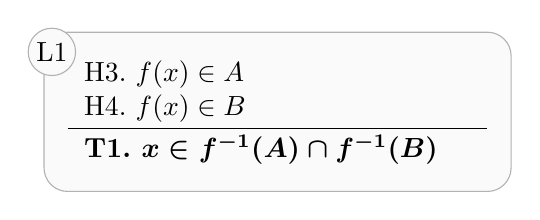
\begin{tikzpicture}[baseline=(main.base)]%
\node[tableau] (main) {%
\\

\begin{tabular}{ll}%
H3.\ $\textrm{$f(x)\in A$}$&\\
H4.\ $\textrm{$f(x)\in B$}$&
\Bstrut\\\hline\Tstrut
\textbf{\boldmath T1.\ $\textrm{$x\in f^{-1}(A)\cap f^{-1}(B)$}$\unboldmath }&\textbf{\boldmath \unboldmath }
\end{tabular}%
};%
\node[tableaulabel] at (main.north west) [xshift=4mm, yshift=-5.5mm] {L1};
\end{tikzpicture}%
\end{fit}
\smallskip

\noindent3. Quantifier-free expansion of target T1.\nopagebreak[4] 
\marginpar{We would like to show that $x\in f^{-1}(A)\cap f^{-1}(B)$, i.e. that $x\in f^{-1}(A)$ and $x\in f^{-1}(B)$.}\nopagebreak[4] 
\smallskip\nopagebreak[4] 

\begin{fit}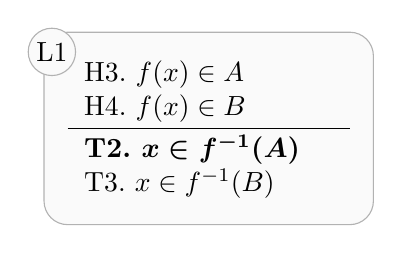
\begin{tikzpicture}[baseline=(main.base)]%
\node[tableau] (main) {%
\\

\begin{tabular}{ll}%
H3.\ $\textrm{$f(x)\in A$}$&\\
H4.\ $\textrm{$f(x)\in B$}$&
\Bstrut\\\hline\Tstrut
\textbf{\boldmath T2.\ $\textrm{$x\in f^{-1}(A)$}$\unboldmath }&\textbf{\boldmath \unboldmath }\\
T3.\ $\textrm{$x\in f^{-1}(B)$}$&
\end{tabular}%
};%
\node[tableaulabel] at (main.north west) [xshift=4mm, yshift=-5.5mm] {L1};
\end{tikzpicture}%
\end{fit}
\smallskip

\noindent4. Quantifier-free expansion of target T2.\nopagebreak[4] 
\marginpar{We would like to show that $x\in f^{-1}(A)$, i.e. that $f(x)\in A$.}\nopagebreak[4] 
\smallskip\nopagebreak[4] 

\begin{fit}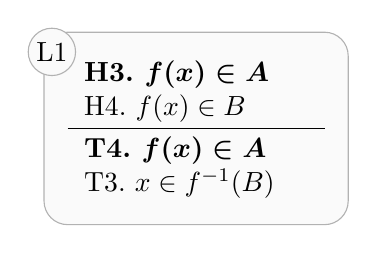
\begin{tikzpicture}[baseline=(main.base)]%
\node[tableau] (main) {%
\\

\begin{tabular}{ll}%
\textbf{\boldmath H3.\ $\textrm{$f(x)\in A$}$\unboldmath }&\textbf{\boldmath \unboldmath }\\
H4.\ $\textrm{$f(x)\in B$}$&
\Bstrut\\\hline\Tstrut
\textbf{\boldmath T4.\ $\textrm{$f(x)\in A$}$\unboldmath }&\textbf{\boldmath \unboldmath }\\
T3.\ $\textrm{$x\in f^{-1}(B)$}$&
\end{tabular}%
};%
\node[tableaulabel] at (main.north west) [xshift=4mm, yshift=-5.5mm] {L1};
\end{tikzpicture}%
\end{fit}
\smallskip

\noindent5. Hypothesis H3 matches target T4, so we can remove T4.\nopagebreak[4] 
\marginpar{}\nopagebreak[4] 
\smallskip\nopagebreak[4] 

\begin{fit}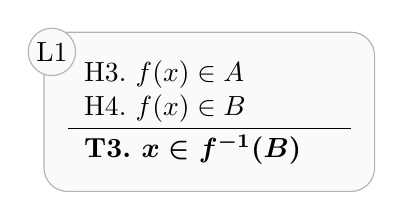
\begin{tikzpicture}[baseline=(main.base)]%
\node[tableau] (main) {%
\\

\begin{tabular}{ll}%
H3.\ $\textrm{$f(x)\in A$}$&\\
H4.\ $\textrm{$f(x)\in B$}$&
\Bstrut\\\hline\Tstrut
\textbf{\boldmath T3.\ $\textrm{$x\in f^{-1}(B)$}$\unboldmath }&\textbf{\boldmath \unboldmath }
\end{tabular}%
};%
\node[tableaulabel] at (main.north west) [xshift=4mm, yshift=-5.5mm] {L1};
\end{tikzpicture}%
\end{fit}
\smallskip

\noindent6. Quantifier-free expansion of target T3.\nopagebreak[4] 
\marginpar{We would like to show that $x\in f^{-1}(B)$, i.e. that $f(x)\in B$.}\nopagebreak[4] 
\smallskip\nopagebreak[4] 

\begin{fit}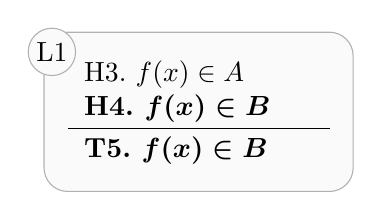
\begin{tikzpicture}[baseline=(main.base)]%
\node[tableau] (main) {%
\\

\begin{tabular}{ll}%
H3.\ $\textrm{$f(x)\in A$}$&\\
\textbf{\boldmath H4.\ $\textrm{$f(x)\in B$}$\unboldmath }&\textbf{\boldmath \unboldmath }
\Bstrut\\\hline\Tstrut
\textbf{\boldmath T5.\ $\textrm{$f(x)\in B$}$\unboldmath }&\textbf{\boldmath \unboldmath }
\end{tabular}%
};%
\node[tableaulabel] at (main.north west) [xshift=4mm, yshift=-5.5mm] {L1};
\end{tikzpicture}%
\end{fit}
\smallskip

\noindent7. Hypothesis H4 matches target T5, so L1 is done.\nopagebreak[4] 
\marginpar{But this is clearly the case, so we are done.}\nopagebreak[4] 
\smallskip\nopagebreak[4] 

\begin{fit}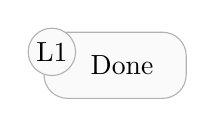
\begin{tikzpicture}%
\node[tableau] (main) {%
\ \ \,Done
};%
\node[tableaulabel] at (main.north west) [xshift=4mm, yshift=-5.5mm] {L1};
\end{tikzpicture}%
\end{fit}

Problem solved.
\cleardoublepage

\end{steps}
{\begin{center} \large \textbf{Prove that $f^{-1}(A) \cap f^{-1}(B) \subseteq f^{-1}(A \cap B)$}\end{center}}\nopagebreak[4]

\begin{center}
\begin{minipage}{120mm}
Let $x$ be an element of $f^{-1}(A)\cap f^{-1}(B)$. Then $x\in f^{-1}(A)$ and $x\in f^{-1}(B)$. Then $f(x)\in A$ and $f(x)\in B$. We would like to show that $x\in f^{-1}(A\cap B)$, i.e. that $f(x)\in A\cap B$. We would like to show that $f(x)\in A\cap B$, i.e. that $f(x)\in A$ and $f(x)\in B$. But this is clearly the case, so we are done.
\end{minipage}
\end{center}

\bigskip
\begin{steps}
\begin{fit}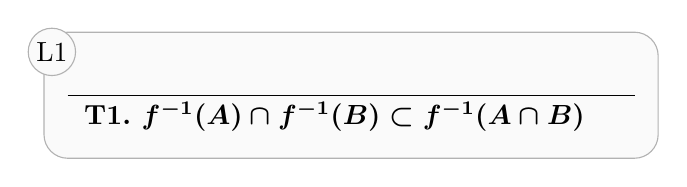
\begin{tikzpicture}[baseline=(main.base)]%
\node[tableau] (main) {%
\\

\begin{tabular}{ll}%

\Bstrut\\\hline\Tstrut
\textbf{\boldmath T1.\ $\textrm{$f^{-1}(A)\cap f^{-1}(B)\subset f^{-1}(A\cap B)$}$\unboldmath }&\textbf{\boldmath \unboldmath }
\end{tabular}%
};%
\node[tableaulabel] at (main.north west) [xshift=4mm, yshift=-5.5mm] {L1};
\end{tikzpicture}%
\end{fit}
\smallskip

\noindent1. Expand pre-universal target T1.\nopagebreak[4] 
\marginpar{}\nopagebreak[4] 
\smallskip\nopagebreak[4] 

\begin{fit}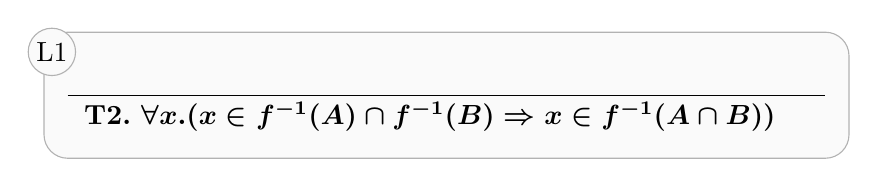
\begin{tikzpicture}[baseline=(main.base)]%
\node[tableau] (main) {%
\\

\begin{tabular}{ll}%

\Bstrut\\\hline\Tstrut
\textbf{\boldmath T2.\ $\forall x.(\textrm{$x\in f^{-1}(A)\cap f^{-1}(B)$}\Rightarrow \textrm{$x\in f^{-1}(A\cap B)$})$\unboldmath }&\textbf{\boldmath \unboldmath }
\end{tabular}%
};%
\node[tableaulabel] at (main.north west) [xshift=4mm, yshift=-5.5mm] {L1};
\end{tikzpicture}%
\end{fit}
\smallskip

\noindent2. Apply `let' trick and move premise of universal-conditional target T2 above the line.\nopagebreak[4] 
\marginpar{Let $x$ be an element of $f^{-1}(A)\cap f^{-1}(B)$.}\nopagebreak[4] 
\smallskip\nopagebreak[4] 

\begin{fit}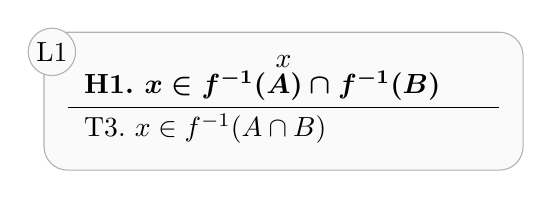
\begin{tikzpicture}[baseline=(main.base)]%
\node[tableau] (main) {%
$x$\\

\begin{tabular}{ll}%
\textbf{\boldmath H1.\ $\textrm{$x\in f^{-1}(A)\cap f^{-1}(B)$}$\unboldmath }&\textbf{\boldmath \unboldmath }
\Bstrut\\\hline\Tstrut
T3.\ $\textrm{$x\in f^{-1}(A\cap B)$}$&
\end{tabular}%
};%
\node[tableaulabel] at (main.north west) [xshift=4mm, yshift=-5.5mm] {L1};
\end{tikzpicture}%
\end{fit}
\smallskip

\noindent3. Quantifier-free expansion of hypothesis H1.\nopagebreak[4] 
\marginpar{Since $x\in f^{-1}(A)\cap f^{-1}(B)$, $x\in f^{-1}(A)$ and $x\in f^{-1}(B)$.}\nopagebreak[4] 
\smallskip\nopagebreak[4] 

\begin{fit}\begin{tikzpicture}[baseline=(main.base)]%
\node[tableau] (main) {%
$x$\\

\begin{tabular}{ll}%
\textbf{\boldmath H2.\ $\textrm{$x\in f^{-1}(A)$}$\unboldmath }&\textbf{\boldmath \unboldmath }\\
H3.\ $\textrm{$x\in f^{-1}(B)$}$&
\Bstrut\\\hline\Tstrut
T3.\ $\textrm{$x\in f^{-1}(A\cap B)$}$&
\end{tabular}%
};%
\node[tableaulabel] at (main.north west) [xshift=4mm, yshift=-5.5mm] {L1};
\end{tikzpicture}%
\end{fit}
\smallskip

\noindent4. Quantifier-free expansion of hypothesis H2.\nopagebreak[4] 
\marginpar{Since $x\in f^{-1}(A)$, we have that $f(x)\in A$.}\nopagebreak[4] 
\smallskip\nopagebreak[4] 

\begin{fit}\begin{tikzpicture}[baseline=(main.base)]%
\node[tableau] (main) {%
$x$\\

\begin{tabular}{ll}%
H4.\ $\textrm{$f(x)\in A$}$&\\
\textbf{\boldmath H3.\ $\textrm{$x\in f^{-1}(B)$}$\unboldmath }&\textbf{\boldmath \unboldmath }
\Bstrut\\\hline\Tstrut
T3.\ $\textrm{$x\in f^{-1}(A\cap B)$}$&
\end{tabular}%
};%
\node[tableaulabel] at (main.north west) [xshift=4mm, yshift=-5.5mm] {L1};
\end{tikzpicture}%
\end{fit}
\smallskip

\noindent5. Quantifier-free expansion of hypothesis H3.\nopagebreak[4] 
\marginpar{Since $x\in f^{-1}(B)$, we have that $f(x)\in B$.}\nopagebreak[4] 
\smallskip\nopagebreak[4] 

\begin{fit}\begin{tikzpicture}[baseline=(main.base)]%
\node[tableau] (main) {%
$x$\\

\begin{tabular}{ll}%
H4.\ $\textrm{$f(x)\in A$}$&\\
H5.\ $\textrm{$f(x)\in B$}$&
\Bstrut\\\hline\Tstrut
\textbf{\boldmath T3.\ $\textrm{$x\in f^{-1}(A\cap B)$}$\unboldmath }&\textbf{\boldmath \unboldmath }
\end{tabular}%
};%
\node[tableaulabel] at (main.north west) [xshift=4mm, yshift=-5.5mm] {L1};
\end{tikzpicture}%
\end{fit}
\smallskip

\noindent6. Quantifier-free expansion of target T3.\nopagebreak[4] 
\marginpar{We would like to show that $x\in f^{-1}(A\cap B)$, i.e. that $f(x)\in A\cap B$.}\nopagebreak[4] 
\smallskip\nopagebreak[4] 

\begin{fit}\begin{tikzpicture}[baseline=(main.base)]%
\node[tableau] (main) {%
$x$\\

\begin{tabular}{ll}%
H4.\ $\textrm{$f(x)\in A$}$&\\
H5.\ $\textrm{$f(x)\in B$}$&
\Bstrut\\\hline\Tstrut
\textbf{\boldmath T4.\ $\textrm{$f(x)\in A\cap B$}$\unboldmath }&\textbf{\boldmath \unboldmath }
\end{tabular}%
};%
\node[tableaulabel] at (main.north west) [xshift=4mm, yshift=-5.5mm] {L1};
\end{tikzpicture}%
\end{fit}
\smallskip

\noindent7. Quantifier-free expansion of target T4.\nopagebreak[4] 
\marginpar{We would like to show that $f(x)\in A\cap B$, i.e. that $f(x)\in A$ and $f(x)\in B$.}\nopagebreak[4] 
\smallskip\nopagebreak[4] 

\begin{fit}\begin{tikzpicture}[baseline=(main.base)]%
\node[tableau] (main) {%
$x$\\

\begin{tabular}{ll}%
\textbf{\boldmath H4.\ $\textrm{$f(x)\in A$}$\unboldmath }&\textbf{\boldmath \unboldmath }\\
H5.\ $\textrm{$f(x)\in B$}$&
\Bstrut\\\hline\Tstrut
\textbf{\boldmath T5.\ $\textrm{$f(x)\in A$}$\unboldmath }&\textbf{\boldmath \unboldmath }\\
T6.\ $\textrm{$f(x)\in B$}$&
\end{tabular}%
};%
\node[tableaulabel] at (main.north west) [xshift=4mm, yshift=-5.5mm] {L1};
\end{tikzpicture}%
\end{fit}
\smallskip

\noindent8. Hypothesis H4 matches target T5, so we can remove T5.\nopagebreak[4] 
\marginpar{}\nopagebreak[4] 
\smallskip\nopagebreak[4] 

\begin{fit}\begin{tikzpicture}[baseline=(main.base)]%
\node[tableau] (main) {%
$x$\\

\begin{tabular}{ll}%
H4.\ $\textrm{$f(x)\in A$}$&\\
\textbf{\boldmath H5.\ $\textrm{$f(x)\in B$}$\unboldmath }&\textbf{\boldmath \unboldmath }
\Bstrut\\\hline\Tstrut
\textbf{\boldmath T6.\ $\textrm{$f(x)\in B$}$\unboldmath }&\textbf{\boldmath \unboldmath }
\end{tabular}%
};%
\node[tableaulabel] at (main.north west) [xshift=4mm, yshift=-5.5mm] {L1};
\end{tikzpicture}%
\end{fit}
\smallskip

\noindent9. Hypothesis H5 matches target T6, so L1 is done.\nopagebreak[4] 
\marginpar{But this is clearly the case, so we are done.}\nopagebreak[4] 
\smallskip\nopagebreak[4] 

\begin{fit}\begin{tikzpicture}%
\node[tableau] (main) {%
\ \ \,Done
};%
\node[tableaulabel] at (main.north west) [xshift=4mm, yshift=-5.5mm] {L1};
\end{tikzpicture}%
\end{fit}

Problem solved.
\cleardoublepage

\end{steps}
{\begin{center} \large \textbf{Prove that $f^{-1}(A \cup B) \subseteq f^{-1}(A) \cup f^{-1}(B)$}\end{center}}\nopagebreak[4]

\begin{center}
\begin{minipage}{120mm}
Let $x$ be an element of $f^{-1}(A\cup B)$. Then $f(x)\in A\cup B$. Then $f(x)\in A$ or $f(x)\in B$. We would like to show that $x\in f^{-1}(A)\cup f^{-1}(B)$, i.e. that $x\in f^{-1}(A)$ or $x\in f^{-1}(B)$. We would like to show that $x\in f^{-1}(A)$, i.e. that $f(x)\in A$. But this is clearly the case, so we are done. We would like to show that $x\in f^{-1}(A)\cup f^{-1}(B)$, i.e. that $x\in f^{-1}(A)$ or $x\in f^{-1}(B)$. We would like to show that $x\in f^{-1}(A)$, i.e. that $f(x)\in A$. We would like to show that $x\in f^{-1}(B)$, i.e. that $f(x)\in B$. But this is clearly the case, so we are done.
\end{minipage}
\end{center}

\bigskip
\begin{steps}
\begin{fit}\begin{tikzpicture}[baseline=(main.base)]%
\node[tableau] (main) {%
\\

\begin{tabular}{ll}%

\Bstrut\\\hline\Tstrut
\textbf{\boldmath T1.\ $\textrm{$f^{-1}(A\cup B)\subset f^{-1}(A)\cup f^{-1}(B)$}$\unboldmath }&\textbf{\boldmath \unboldmath }
\end{tabular}%
};%
\node[tableaulabel] at (main.north west) [xshift=4mm, yshift=-5.5mm] {L1};
\end{tikzpicture}%
\end{fit}
\smallskip

\noindent1. Expand pre-universal target T1.\nopagebreak[4] 
\marginpar{}\nopagebreak[4] 
\smallskip\nopagebreak[4] 

\begin{fit}\begin{tikzpicture}[baseline=(main.base)]%
\node[tableau] (main) {%
\\

\begin{tabular}{ll}%

\Bstrut\\\hline\Tstrut
\textbf{\boldmath T2.\ $\forall x.(\textrm{$x\in f^{-1}(A\cup B)$}\Rightarrow \textrm{$x\in f^{-1}(A)\cup f^{-1}(B)$})$\unboldmath }&\textbf{\boldmath \unboldmath }
\end{tabular}%
};%
\node[tableaulabel] at (main.north west) [xshift=4mm, yshift=-5.5mm] {L1};
\end{tikzpicture}%
\end{fit}
\smallskip

\noindent2. Apply `let' trick and move premise of universal-conditional target T2 above the line.\nopagebreak[4] 
\marginpar{Let $x$ be an element of $f^{-1}(A\cup B)$.}\nopagebreak[4] 
\smallskip\nopagebreak[4] 

\begin{fit}\begin{tikzpicture}[baseline=(main.base)]%
\node[tableau] (main) {%
$x$\\

\begin{tabular}{ll}%
\textbf{\boldmath H1.\ $\textrm{$x\in f^{-1}(A\cup B)$}$\unboldmath }&\textbf{\boldmath \unboldmath }
\Bstrut\\\hline\Tstrut
T3.\ $\textrm{$x\in f^{-1}(A)\cup f^{-1}(B)$}$&
\end{tabular}%
};%
\node[tableaulabel] at (main.north west) [xshift=4mm, yshift=-5.5mm] {L1};
\end{tikzpicture}%
\end{fit}
\smallskip

\noindent3. Quantifier-free expansion of hypothesis H1.\nopagebreak[4] 
\marginpar{Since $x\in f^{-1}(A\cup B)$, we have that $f(x)\in A\cup B$.}\nopagebreak[4] 
\smallskip\nopagebreak[4] 

\begin{fit}\begin{tikzpicture}[baseline=(main.base)]%
\node[tableau] (main) {%
$x$\\

\begin{tabular}{ll}%
\textbf{\boldmath H2.\ $\textrm{$f(x)\in A\cup B$}$\unboldmath }&\textbf{\boldmath \unboldmath }
\Bstrut\\\hline\Tstrut
T3.\ $\textrm{$x\in f^{-1}(A)\cup f^{-1}(B)$}$&
\end{tabular}%
};%
\node[tableaulabel] at (main.north west) [xshift=4mm, yshift=-5.5mm] {L1};
\end{tikzpicture}%
\end{fit}
\smallskip

\noindent4. Quantifier-free expansion of hypothesis H2.\nopagebreak[4] 
\marginpar{Since $f(x)\in A\cup B$, $f(x)\in A$ or $f(x)\in B$.}\nopagebreak[4] 
\smallskip\nopagebreak[4] 

\begin{fit}\begin{tikzpicture}[baseline=(main.base)]%
\node[tableau] (main) {%
$x$\\

\begin{tabular}{ll}%
\textbf{\boldmath H3.\ $\textrm{$f(x)\in A$}\vee \textrm{$f(x)\in B$}$\unboldmath }&\textbf{\boldmath \unboldmath }
\Bstrut\\\hline\Tstrut
T3.\ $\textrm{$x\in f^{-1}(A)\cup f^{-1}(B)$}$&
\end{tabular}%
};%
\node[tableaulabel] at (main.north west) [xshift=4mm, yshift=-5.5mm] {L1};
\end{tikzpicture}%
\end{fit}
\smallskip

\noindent5. Split into cases to handle disjunctive hypothesis H3.\nopagebreak[4] 
\marginpar{}\nopagebreak[4] 
\smallskip\nopagebreak[4] 

\begin{fit}\begin{tikzpicture}[baseline=(main.base)]%
\node[tableau] (main) {%
$x$\\

\begin{tabular}{ll}%

\Bstrut\\\hline\Tstrut
\begin{tikzpicture}[baseline=(main.base)]%
\node[tableau] (main) {%
\\

\begin{tabular}{ll}%
H4.\ $\textrm{$f(x)\in A$}$&
\Bstrut\\\hline\Tstrut
\textbf{\boldmath T4.\ $\textrm{$x\in f^{-1}(A)\cup f^{-1}(B)$}$\unboldmath }&\textbf{\boldmath \unboldmath }
\end{tabular}%
};%
\node[tableaulabel] at (main.north west) [xshift=4mm, yshift=-5.5mm] {L2};
\end{tikzpicture}%
\\
\begin{tikzpicture}[baseline=(main.base)]%
\node[tableau] (main) {%
\\

\begin{tabular}{ll}%
H5.\ $\textrm{$f(x)\in B$}$&
\Bstrut\\\hline\Tstrut
T5.\ $\textrm{$x\in f^{-1}(A)\cup f^{-1}(B)$}$&
\end{tabular}%
};%
\node[tableaulabel] at (main.north west) [xshift=4mm, yshift=-5.5mm] {L3};
\end{tikzpicture}%

\end{tabular}%
};%
\node[tableaulabel] at (main.north west) [xshift=4mm, yshift=-5.5mm] {L1};
\end{tikzpicture}%
\end{fit}
\smallskip

\noindent6. Quantifier-free expansion of target T4.\nopagebreak[4] 
\marginpar{We would like to show that $x\in f^{-1}(A)\cup f^{-1}(B)$, i.e. that $x\in f^{-1}(A)$ or $x\in f^{-1}(B)$.}\nopagebreak[4] 
\smallskip\nopagebreak[4] 

\begin{fit}\begin{tikzpicture}[baseline=(main.base)]%
\node[tableau] (main) {%
$x$\\

\begin{tabular}{ll}%

\Bstrut\\\hline\Tstrut
\begin{tikzpicture}[baseline=(main.base)]%
\node[tableau] (main) {%
\\

\begin{tabular}{ll}%
H4.\ $\textrm{$f(x)\in A$}$&
\Bstrut\\\hline\Tstrut
\textbf{\boldmath T6.\ $\textrm{$x\in f^{-1}(A)$}\vee \textrm{$x\in f^{-1}(B)$}$\unboldmath }&\textbf{\boldmath \unboldmath }
\end{tabular}%
};%
\node[tableaulabel] at (main.north west) [xshift=4mm, yshift=-5.5mm] {L2};
\end{tikzpicture}%
\\
\begin{tikzpicture}[baseline=(main.base)]%
\node[tableau] (main) {%
\\

\begin{tabular}{ll}%
H5.\ $\textrm{$f(x)\in B$}$&
\Bstrut\\\hline\Tstrut
T5.\ $\textrm{$x\in f^{-1}(A)\cup f^{-1}(B)$}$&
\end{tabular}%
};%
\node[tableaulabel] at (main.north west) [xshift=4mm, yshift=-5.5mm] {L3};
\end{tikzpicture}%

\end{tabular}%
};%
\node[tableaulabel] at (main.north west) [xshift=4mm, yshift=-5.5mm] {L1};
\end{tikzpicture}%
\end{fit}
\smallskip

\noindent7. Split up disjunctive target T6.\nopagebreak[4] 
\marginpar{}\nopagebreak[4] 
\smallskip\nopagebreak[4] 

\begin{fit}\begin{tikzpicture}[baseline=(main.base)]%
\node[tableau] (main) {%
$x$\\

\begin{tabular}{ll}%

\Bstrut\\\hline\Tstrut
\begin{tikzpicture}[baseline=(main.base)]%
\node[tableau] (main) {%
\\

\begin{tabular}{ll}%
H4.\ $\textrm{$f(x)\in A$}$&
\Bstrut\\\hline\Tstrut
\begin{tikzpicture}[baseline=(main.base)]%
\node[tableau] (main) {%
\\

\begin{tabular}{ll}%

\Bstrut\\\hline\Tstrut
\textbf{\boldmath T9.\ $\textrm{$x\in f^{-1}(A)$}$\unboldmath }&\textbf{\boldmath \unboldmath }
\end{tabular}%
};%
\node[tableaulabel] at (main.north west) [xshift=4mm, yshift=-5.5mm] {L6};
\end{tikzpicture}%
\hspace{2mm}$\vee$\begin{tikzpicture}[baseline=(main.base)]%
\node[tableau] (main) {%
\\

\begin{tabular}{ll}%

\Bstrut\\\hline\Tstrut
T10.\ $\textrm{$x\in f^{-1}(B)$}$&
\end{tabular}%
};%
\node[tableaulabel] at (main.north west) [xshift=4mm, yshift=-5.5mm] {L7};
\end{tikzpicture}%

\end{tabular}%
};%
\node[tableaulabel] at (main.north west) [xshift=4mm, yshift=-5.5mm] {L2};
\end{tikzpicture}%
\\
\begin{tikzpicture}[baseline=(main.base)]%
\node[tableau] (main) {%
\\

\begin{tabular}{ll}%
H5.\ $\textrm{$f(x)\in B$}$&
\Bstrut\\\hline\Tstrut
T5.\ $\textrm{$x\in f^{-1}(A)\cup f^{-1}(B)$}$&
\end{tabular}%
};%
\node[tableaulabel] at (main.north west) [xshift=4mm, yshift=-5.5mm] {L3};
\end{tikzpicture}%

\end{tabular}%
};%
\node[tableaulabel] at (main.north west) [xshift=4mm, yshift=-5.5mm] {L1};
\end{tikzpicture}%
\end{fit}
\smallskip

\noindent8. Quantifier-free expansion of target T9.\nopagebreak[4] 
\marginpar{We would like to show that $x\in f^{-1}(A)$, i.e. that $f(x)\in A$.}\nopagebreak[4] 
\smallskip\nopagebreak[4] 

\begin{fit}\begin{tikzpicture}[baseline=(main.base)]%
\node[tableau] (main) {%
$x$\\

\begin{tabular}{ll}%

\Bstrut\\\hline\Tstrut
\begin{tikzpicture}[baseline=(main.base)]%
\node[tableau] (main) {%
\\

\begin{tabular}{ll}%
\textbf{\boldmath H4.\ $\textrm{$f(x)\in A$}$\unboldmath }&\textbf{\boldmath \unboldmath }
\Bstrut\\\hline\Tstrut
\begin{tikzpicture}[baseline=(main.base)]%
\node[tableau] (main) {%
\\

\begin{tabular}{ll}%

\Bstrut\\\hline\Tstrut
\textbf{\boldmath T11.\ $\textrm{$f(x)\in A$}$\unboldmath }&\textbf{\boldmath \unboldmath }
\end{tabular}%
};%
\node[tableaulabel] at (main.north west) [xshift=4mm, yshift=-5.5mm] {L6};
\end{tikzpicture}%
\hspace{2mm}$\vee$\begin{tikzpicture}[baseline=(main.base)]%
\node[tableau] (main) {%
\\

\begin{tabular}{ll}%

\Bstrut\\\hline\Tstrut
T10.\ $\textrm{$x\in f^{-1}(B)$}$&
\end{tabular}%
};%
\node[tableaulabel] at (main.north west) [xshift=4mm, yshift=-5.5mm] {L7};
\end{tikzpicture}%

\end{tabular}%
};%
\node[tableaulabel] at (main.north west) [xshift=4mm, yshift=-5.5mm] {L2};
\end{tikzpicture}%
\\
\begin{tikzpicture}[baseline=(main.base)]%
\node[tableau] (main) {%
\\

\begin{tabular}{ll}%
H5.\ $\textrm{$f(x)\in B$}$&
\Bstrut\\\hline\Tstrut
T5.\ $\textrm{$x\in f^{-1}(A)\cup f^{-1}(B)$}$&
\end{tabular}%
};%
\node[tableaulabel] at (main.north west) [xshift=4mm, yshift=-5.5mm] {L3};
\end{tikzpicture}%

\end{tabular}%
};%
\node[tableaulabel] at (main.north west) [xshift=4mm, yshift=-5.5mm] {L1};
\end{tikzpicture}%
\end{fit}
\smallskip

\noindent9. Hypothesis H4 matches target T11, so L6 is done.\nopagebreak[4] 
\marginpar{But this is clearly the case, so we are done.}\nopagebreak[4] 
\smallskip\nopagebreak[4] 

\begin{fit}\begin{tikzpicture}[baseline=(main.base)]%
\node[tableau] (main) {%
$x$\\

\begin{tabular}{ll}%

\Bstrut\\\hline\Tstrut
\begin{tikzpicture}[baseline=(main.base)]%
\node[tableau] (main) {%
\\

\begin{tabular}{ll}%
H4.\ $\textrm{$f(x)\in A$}$&
\Bstrut\\\hline\Tstrut
\begin{tikzpicture}%
\node[tableau] (main) {%
\ \ \,Done
};%
\node[tableaulabel] at (main.north west) [xshift=4mm, yshift=-5.5mm] {L6};
\end{tikzpicture}%
\hspace{2mm}$\vee$\begin{tikzpicture}[baseline=(main.base)]%
\node[tableau] (main) {%
\\

\begin{tabular}{ll}%

\Bstrut\\\hline\Tstrut
T10.\ $\textrm{$x\in f^{-1}(B)$}$&
\end{tabular}%
};%
\node[tableaulabel] at (main.north west) [xshift=4mm, yshift=-5.5mm] {L7};
\end{tikzpicture}%

\end{tabular}%
};%
\node[tableaulabel] at (main.north west) [xshift=4mm, yshift=-5.5mm] {L2};
\end{tikzpicture}%
\\
\begin{tikzpicture}[baseline=(main.base)]%
\node[tableau] (main) {%
\\

\begin{tabular}{ll}%
H5.\ $\textrm{$f(x)\in B$}$&
\Bstrut\\\hline\Tstrut
T5.\ $\textrm{$x\in f^{-1}(A)\cup f^{-1}(B)$}$&
\end{tabular}%
};%
\node[tableaulabel] at (main.north west) [xshift=4mm, yshift=-5.5mm] {L3};
\end{tikzpicture}%

\end{tabular}%
};%
\node[tableaulabel] at (main.north west) [xshift=4mm, yshift=-5.5mm] {L1};
\end{tikzpicture}%
\end{fit}
\smallskip

\noindent10. Some disjunct of the target of L2 is `Done', so L2 is itself `Done'.\nopagebreak[4] 
\marginpar{}\nopagebreak[4] 
\smallskip\nopagebreak[4] 

\begin{fit}\begin{tikzpicture}[baseline=(main.base)]%
\node[tableau] (main) {%
$x$\\

\begin{tabular}{ll}%

\Bstrut\\\hline\Tstrut
\begin{tikzpicture}%
\node[tableau] (main) {%
\ \ \,Done
};%
\node[tableaulabel] at (main.north west) [xshift=4mm, yshift=-5.5mm] {L2};
\end{tikzpicture}%
\\
\begin{tikzpicture}[baseline=(main.base)]%
\node[tableau] (main) {%
\\

\begin{tabular}{ll}%
H5.\ $\textrm{$f(x)\in B$}$&
\Bstrut\\\hline\Tstrut
T5.\ $\textrm{$x\in f^{-1}(A)\cup f^{-1}(B)$}$&
\end{tabular}%
};%
\node[tableaulabel] at (main.north west) [xshift=4mm, yshift=-5.5mm] {L3};
\end{tikzpicture}%

\end{tabular}%
};%
\node[tableaulabel] at (main.north west) [xshift=4mm, yshift=-5.5mm] {L1};
\end{tikzpicture}%
\end{fit}
\smallskip

\noindent11. Remove `Done' targets of L1.\nopagebreak[4] 
\marginpar{}\nopagebreak[4] 
\smallskip\nopagebreak[4] 

\begin{fit}\begin{tikzpicture}[baseline=(main.base)]%
\node[tableau] (main) {%
$x$\\

\begin{tabular}{ll}%

\Bstrut\\\hline\Tstrut
\begin{tikzpicture}[baseline=(main.base)]%
\node[tableau] (main) {%
\\

\begin{tabular}{ll}%
H5.\ $\textrm{$f(x)\in B$}$&
\Bstrut\\\hline\Tstrut
\textbf{\boldmath T5.\ $\textrm{$x\in f^{-1}(A)\cup f^{-1}(B)$}$\unboldmath }&\textbf{\boldmath \unboldmath }
\end{tabular}%
};%
\node[tableaulabel] at (main.north west) [xshift=4mm, yshift=-5.5mm] {L3};
\end{tikzpicture}%

\end{tabular}%
};%
\node[tableaulabel] at (main.north west) [xshift=4mm, yshift=-5.5mm] {L1};
\end{tikzpicture}%
\end{fit}
\smallskip

\noindent12. Quantifier-free expansion of target T5.\nopagebreak[4] 
\marginpar{We would like to show that $x\in f^{-1}(A)\cup f^{-1}(B)$, i.e. that $x\in f^{-1}(A)$ or $x\in f^{-1}(B)$.}\nopagebreak[4] 
\smallskip\nopagebreak[4] 

\begin{fit}\begin{tikzpicture}[baseline=(main.base)]%
\node[tableau] (main) {%
$x$\\

\begin{tabular}{ll}%

\Bstrut\\\hline\Tstrut
\begin{tikzpicture}[baseline=(main.base)]%
\node[tableau] (main) {%
\\

\begin{tabular}{ll}%
H5.\ $\textrm{$f(x)\in B$}$&
\Bstrut\\\hline\Tstrut
\textbf{\boldmath T12.\ $\textrm{$x\in f^{-1}(A)$}\vee \textrm{$x\in f^{-1}(B)$}$\unboldmath }&\textbf{\boldmath \unboldmath }
\end{tabular}%
};%
\node[tableaulabel] at (main.north west) [xshift=4mm, yshift=-5.5mm] {L3};
\end{tikzpicture}%

\end{tabular}%
};%
\node[tableaulabel] at (main.north west) [xshift=4mm, yshift=-5.5mm] {L1};
\end{tikzpicture}%
\end{fit}
\smallskip

\noindent13. Split up disjunctive target T12.\nopagebreak[4] 
\marginpar{}\nopagebreak[4] 
\smallskip\nopagebreak[4] 

\begin{fit}\begin{tikzpicture}[baseline=(main.base)]%
\node[tableau] (main) {%
$x$\\

\begin{tabular}{ll}%

\Bstrut\\\hline\Tstrut
\begin{tikzpicture}[baseline=(main.base)]%
\node[tableau] (main) {%
\\

\begin{tabular}{ll}%
H5.\ $\textrm{$f(x)\in B$}$&
\Bstrut\\\hline\Tstrut
\begin{tikzpicture}[baseline=(main.base)]%
\node[tableau] (main) {%
\\

\begin{tabular}{ll}%

\Bstrut\\\hline\Tstrut
\textbf{\boldmath T15.\ $\textrm{$x\in f^{-1}(A)$}$\unboldmath }&\textbf{\boldmath \unboldmath }
\end{tabular}%
};%
\node[tableaulabel] at (main.north west) [xshift=4mm, yshift=-5.5mm] {L10};
\end{tikzpicture}%
\hspace{2mm}$\vee$\begin{tikzpicture}[baseline=(main.base)]%
\node[tableau] (main) {%
\\

\begin{tabular}{ll}%

\Bstrut\\\hline\Tstrut
T16.\ $\textrm{$x\in f^{-1}(B)$}$&
\end{tabular}%
};%
\node[tableaulabel] at (main.north west) [xshift=4mm, yshift=-5.5mm] {L11};
\end{tikzpicture}%

\end{tabular}%
};%
\node[tableaulabel] at (main.north west) [xshift=4mm, yshift=-5.5mm] {L3};
\end{tikzpicture}%

\end{tabular}%
};%
\node[tableaulabel] at (main.north west) [xshift=4mm, yshift=-5.5mm] {L1};
\end{tikzpicture}%
\end{fit}
\smallskip

\noindent14. Quantifier-free expansion of target T15.\nopagebreak[4] 
\marginpar{We would like to show that $x\in f^{-1}(A)$, i.e. that $f(x)\in A$.}\nopagebreak[4] 
\smallskip\nopagebreak[4] 

\begin{fit}\begin{tikzpicture}[baseline=(main.base)]%
\node[tableau] (main) {%
$x$\\

\begin{tabular}{ll}%

\Bstrut\\\hline\Tstrut
\begin{tikzpicture}[baseline=(main.base)]%
\node[tableau] (main) {%
\\

\begin{tabular}{ll}%
H5.\ $\textrm{$f(x)\in B$}$&
\Bstrut\\\hline\Tstrut
\begin{tikzpicture}[baseline=(main.base)]%
\node[tableau] (main) {%
\\

\begin{tabular}{ll}%

\Bstrut\\\hline\Tstrut
T17.\ $\textrm{$f(x)\in A$}$&
\end{tabular}%
};%
\node[tableaulabel] at (main.north west) [xshift=4mm, yshift=-5.5mm] {L10};
\end{tikzpicture}%
\hspace{2mm}$\vee$\begin{tikzpicture}[baseline=(main.base)]%
\node[tableau] (main) {%
\\

\begin{tabular}{ll}%

\Bstrut\\\hline\Tstrut
\textbf{\boldmath T16.\ $\textrm{$x\in f^{-1}(B)$}$\unboldmath }&\textbf{\boldmath \unboldmath }
\end{tabular}%
};%
\node[tableaulabel] at (main.north west) [xshift=4mm, yshift=-5.5mm] {L11};
\end{tikzpicture}%

\end{tabular}%
};%
\node[tableaulabel] at (main.north west) [xshift=4mm, yshift=-5.5mm] {L3};
\end{tikzpicture}%

\end{tabular}%
};%
\node[tableaulabel] at (main.north west) [xshift=4mm, yshift=-5.5mm] {L1};
\end{tikzpicture}%
\end{fit}
\smallskip

\noindent15. Quantifier-free expansion of target T16.\nopagebreak[4] 
\marginpar{We would like to show that $x\in f^{-1}(B)$, i.e. that $f(x)\in B$.}\nopagebreak[4] 
\smallskip\nopagebreak[4] 

\begin{fit}\begin{tikzpicture}[baseline=(main.base)]%
\node[tableau] (main) {%
$x$\\

\begin{tabular}{ll}%

\Bstrut\\\hline\Tstrut
\begin{tikzpicture}[baseline=(main.base)]%
\node[tableau] (main) {%
\\

\begin{tabular}{ll}%
\textbf{\boldmath H5.\ $\textrm{$f(x)\in B$}$\unboldmath }&\textbf{\boldmath \unboldmath }
\Bstrut\\\hline\Tstrut
\begin{tikzpicture}[baseline=(main.base)]%
\node[tableau] (main) {%
\\

\begin{tabular}{ll}%

\Bstrut\\\hline\Tstrut
T17.\ $\textrm{$f(x)\in A$}$&
\end{tabular}%
};%
\node[tableaulabel] at (main.north west) [xshift=4mm, yshift=-5.5mm] {L10};
\end{tikzpicture}%
\hspace{2mm}$\vee$\begin{tikzpicture}[baseline=(main.base)]%
\node[tableau] (main) {%
\\

\begin{tabular}{ll}%

\Bstrut\\\hline\Tstrut
\textbf{\boldmath T18.\ $\textrm{$f(x)\in B$}$\unboldmath }&\textbf{\boldmath \unboldmath }
\end{tabular}%
};%
\node[tableaulabel] at (main.north west) [xshift=4mm, yshift=-5.5mm] {L11};
\end{tikzpicture}%

\end{tabular}%
};%
\node[tableaulabel] at (main.north west) [xshift=4mm, yshift=-5.5mm] {L3};
\end{tikzpicture}%

\end{tabular}%
};%
\node[tableaulabel] at (main.north west) [xshift=4mm, yshift=-5.5mm] {L1};
\end{tikzpicture}%
\end{fit}
\smallskip

\noindent16. Hypothesis H5 matches target T18, so L11 is done.\nopagebreak[4] 
\marginpar{But this is clearly the case, so we are done.}\nopagebreak[4] 
\smallskip\nopagebreak[4] 

\begin{fit}\begin{tikzpicture}[baseline=(main.base)]%
\node[tableau] (main) {%
$x$\\

\begin{tabular}{ll}%

\Bstrut\\\hline\Tstrut
\begin{tikzpicture}[baseline=(main.base)]%
\node[tableau] (main) {%
\\

\begin{tabular}{ll}%
H5.\ $\textrm{$f(x)\in B$}$&
\Bstrut\\\hline\Tstrut
\begin{tikzpicture}[baseline=(main.base)]%
\node[tableau] (main) {%
\\

\begin{tabular}{ll}%

\Bstrut\\\hline\Tstrut
T17.\ $\textrm{$f(x)\in A$}$&
\end{tabular}%
};%
\node[tableaulabel] at (main.north west) [xshift=4mm, yshift=-5.5mm] {L10};
\end{tikzpicture}%
\hspace{2mm}$\vee$\begin{tikzpicture}%
\node[tableau] (main) {%
\ \ \,Done
};%
\node[tableaulabel] at (main.north west) [xshift=4mm, yshift=-5.5mm] {L11};
\end{tikzpicture}%

\end{tabular}%
};%
\node[tableaulabel] at (main.north west) [xshift=4mm, yshift=-5.5mm] {L3};
\end{tikzpicture}%

\end{tabular}%
};%
\node[tableaulabel] at (main.north west) [xshift=4mm, yshift=-5.5mm] {L1};
\end{tikzpicture}%
\end{fit}
\smallskip

\noindent17. Some disjunct of the target of L3 is `Done', so L3 is itself `Done'.\nopagebreak[4] 
\marginpar{}\nopagebreak[4] 
\smallskip\nopagebreak[4] 

\begin{fit}\begin{tikzpicture}[baseline=(main.base)]%
\node[tableau] (main) {%
$x$\\

\begin{tabular}{ll}%

\Bstrut\\\hline\Tstrut
\begin{tikzpicture}%
\node[tableau] (main) {%
\ \ \,Done
};%
\node[tableaulabel] at (main.north west) [xshift=4mm, yshift=-5.5mm] {L3};
\end{tikzpicture}%

\end{tabular}%
};%
\node[tableaulabel] at (main.north west) [xshift=4mm, yshift=-5.5mm] {L1};
\end{tikzpicture}%
\end{fit}
\smallskip

\noindent18. All targets of L1 are `Done', so L1 is itself done.\nopagebreak[4] 
\marginpar{}\nopagebreak[4] 
\smallskip\nopagebreak[4] 

\begin{fit}\begin{tikzpicture}%
\node[tableau] (main) {%
\ \ \,Done
};%
\node[tableaulabel] at (main.north west) [xshift=4mm, yshift=-5.5mm] {L1};
\end{tikzpicture}%
\end{fit}

Problem solved.
\cleardoublepage

\end{steps}
{\begin{center} \large \textbf{Prove that $f^{-1}(A) \cup f^{-1}(B) \subseteq f^{-1}(A \cup B)$}\end{center}}\nopagebreak[4]

\begin{center}
\begin{minipage}{120mm}
Let $x$ be an element of $f^{-1}(A)\cup f^{-1}(B)$. Then $x\in f^{-1}(A)$ or $x\in f^{-1}(B)$. Since $x\in f^{-1}(A)$, we have that $f(x)\in A$. Since $x\in f^{-1}(B)$, we have that $f(x)\in B$. We would like to show that $x\in f^{-1}(A\cup B)$, i.e. that $f(x)\in A\cup B$. We would like to show that $f(x)\in A\cup B$, i.e. that $f(x)\in A$ or $f(x)\in B$. But this is clearly the case, so we are done. We would like to show that $x\in f^{-1}(A\cup B)$, i.e. that $f(x)\in A\cup B$. We would like to show that $f(x)\in A\cup B$, i.e. that $f(x)\in A$ or $f(x)\in B$. But this is clearly the case, so we are done.
\end{minipage}
\end{center}

\bigskip
\begin{steps}
\begin{fit}\begin{tikzpicture}[baseline=(main.base)]%
\node[tableau] (main) {%
\\

\begin{tabular}{ll}%

\Bstrut\\\hline\Tstrut
\textbf{\boldmath T1.\ $\textrm{$f^{-1}(A)\cup f^{-1}(B)\subset f^{-1}(A\cup B)$}$\unboldmath }&\textbf{\boldmath \unboldmath }
\end{tabular}%
};%
\node[tableaulabel] at (main.north west) [xshift=4mm, yshift=-5.5mm] {L1};
\end{tikzpicture}%
\end{fit}
\smallskip

\noindent1. Expand pre-universal target T1.\nopagebreak[4] 
\marginpar{}\nopagebreak[4] 
\smallskip\nopagebreak[4] 

\begin{fit}\begin{tikzpicture}[baseline=(main.base)]%
\node[tableau] (main) {%
\\

\begin{tabular}{ll}%

\Bstrut\\\hline\Tstrut
\textbf{\boldmath T2.\ $\forall x.(\textrm{$x\in f^{-1}(A)\cup f^{-1}(B)$}\Rightarrow \textrm{$x\in f^{-1}(A\cup B)$})$\unboldmath }&\textbf{\boldmath \unboldmath }
\end{tabular}%
};%
\node[tableaulabel] at (main.north west) [xshift=4mm, yshift=-5.5mm] {L1};
\end{tikzpicture}%
\end{fit}
\smallskip

\noindent2. Apply `let' trick and move premise of universal-conditional target T2 above the line.\nopagebreak[4] 
\marginpar{Let $x$ be an element of $f^{-1}(A)\cup f^{-1}(B)$.}\nopagebreak[4] 
\smallskip\nopagebreak[4] 

\begin{fit}\begin{tikzpicture}[baseline=(main.base)]%
\node[tableau] (main) {%
$x$\\

\begin{tabular}{ll}%
\textbf{\boldmath H1.\ $\textrm{$x\in f^{-1}(A)\cup f^{-1}(B)$}$\unboldmath }&\textbf{\boldmath \unboldmath }
\Bstrut\\\hline\Tstrut
T3.\ $\textrm{$x\in f^{-1}(A\cup B)$}$&
\end{tabular}%
};%
\node[tableaulabel] at (main.north west) [xshift=4mm, yshift=-5.5mm] {L1};
\end{tikzpicture}%
\end{fit}
\smallskip

\noindent3. Quantifier-free expansion of hypothesis H1.\nopagebreak[4] 
\marginpar{Since $x\in f^{-1}(A)\cup f^{-1}(B)$, $x\in f^{-1}(A)$ or $x\in f^{-1}(B)$.}\nopagebreak[4] 
\smallskip\nopagebreak[4] 

\begin{fit}\begin{tikzpicture}[baseline=(main.base)]%
\node[tableau] (main) {%
$x$\\

\begin{tabular}{ll}%
\textbf{\boldmath H2.\ $\textrm{$x\in f^{-1}(A)$}\vee \textrm{$x\in f^{-1}(B)$}$\unboldmath }&\textbf{\boldmath \unboldmath }
\Bstrut\\\hline\Tstrut
T3.\ $\textrm{$x\in f^{-1}(A\cup B)$}$&
\end{tabular}%
};%
\node[tableaulabel] at (main.north west) [xshift=4mm, yshift=-5.5mm] {L1};
\end{tikzpicture}%
\end{fit}
\smallskip

\noindent4. Split into cases to handle disjunctive hypothesis H2.\nopagebreak[4] 
\marginpar{}\nopagebreak[4] 
\smallskip\nopagebreak[4] 

\begin{fit}\begin{tikzpicture}[baseline=(main.base)]%
\node[tableau] (main) {%
$x$\\

\begin{tabular}{ll}%

\Bstrut\\\hline\Tstrut
\begin{tikzpicture}[baseline=(main.base)]%
\node[tableau] (main) {%
\\

\begin{tabular}{ll}%
\textbf{\boldmath H3.\ $\textrm{$x\in f^{-1}(A)$}$\unboldmath }&\textbf{\boldmath \unboldmath }
\Bstrut\\\hline\Tstrut
T4.\ $\textrm{$x\in f^{-1}(A\cup B)$}$&
\end{tabular}%
};%
\node[tableaulabel] at (main.north west) [xshift=4mm, yshift=-5.5mm] {L2};
\end{tikzpicture}%
\\
\begin{tikzpicture}[baseline=(main.base)]%
\node[tableau] (main) {%
\\

\begin{tabular}{ll}%
H4.\ $\textrm{$x\in f^{-1}(B)$}$&
\Bstrut\\\hline\Tstrut
T5.\ $\textrm{$x\in f^{-1}(A\cup B)$}$&
\end{tabular}%
};%
\node[tableaulabel] at (main.north west) [xshift=4mm, yshift=-5.5mm] {L3};
\end{tikzpicture}%

\end{tabular}%
};%
\node[tableaulabel] at (main.north west) [xshift=4mm, yshift=-5.5mm] {L1};
\end{tikzpicture}%
\end{fit}
\smallskip

\noindent5. Quantifier-free expansion of hypothesis H3.\nopagebreak[4] 
\marginpar{Since $x\in f^{-1}(A)$, we have that $f(x)\in A$.}\nopagebreak[4] 
\smallskip\nopagebreak[4] 

\begin{fit}\begin{tikzpicture}[baseline=(main.base)]%
\node[tableau] (main) {%
$x$\\

\begin{tabular}{ll}%

\Bstrut\\\hline\Tstrut
\begin{tikzpicture}[baseline=(main.base)]%
\node[tableau] (main) {%
\\

\begin{tabular}{ll}%
H5.\ $\textrm{$f(x)\in A$}$&
\Bstrut\\\hline\Tstrut
T4.\ $\textrm{$x\in f^{-1}(A\cup B)$}$&
\end{tabular}%
};%
\node[tableaulabel] at (main.north west) [xshift=4mm, yshift=-5.5mm] {L2};
\end{tikzpicture}%
\\
\begin{tikzpicture}[baseline=(main.base)]%
\node[tableau] (main) {%
\\

\begin{tabular}{ll}%
\textbf{\boldmath H4.\ $\textrm{$x\in f^{-1}(B)$}$\unboldmath }&\textbf{\boldmath \unboldmath }
\Bstrut\\\hline\Tstrut
T5.\ $\textrm{$x\in f^{-1}(A\cup B)$}$&
\end{tabular}%
};%
\node[tableaulabel] at (main.north west) [xshift=4mm, yshift=-5.5mm] {L3};
\end{tikzpicture}%

\end{tabular}%
};%
\node[tableaulabel] at (main.north west) [xshift=4mm, yshift=-5.5mm] {L1};
\end{tikzpicture}%
\end{fit}
\smallskip

\noindent6. Quantifier-free expansion of hypothesis H4.\nopagebreak[4] 
\marginpar{Since $x\in f^{-1}(B)$, we have that $f(x)\in B$.}\nopagebreak[4] 
\smallskip\nopagebreak[4] 

\begin{fit}\begin{tikzpicture}[baseline=(main.base)]%
\node[tableau] (main) {%
$x$\\

\begin{tabular}{ll}%

\Bstrut\\\hline\Tstrut
\begin{tikzpicture}[baseline=(main.base)]%
\node[tableau] (main) {%
\\

\begin{tabular}{ll}%
H5.\ $\textrm{$f(x)\in A$}$&
\Bstrut\\\hline\Tstrut
\textbf{\boldmath T4.\ $\textrm{$x\in f^{-1}(A\cup B)$}$\unboldmath }&\textbf{\boldmath \unboldmath }
\end{tabular}%
};%
\node[tableaulabel] at (main.north west) [xshift=4mm, yshift=-5.5mm] {L2};
\end{tikzpicture}%
\\
\begin{tikzpicture}[baseline=(main.base)]%
\node[tableau] (main) {%
\\

\begin{tabular}{ll}%
H6.\ $\textrm{$f(x)\in B$}$&
\Bstrut\\\hline\Tstrut
T5.\ $\textrm{$x\in f^{-1}(A\cup B)$}$&
\end{tabular}%
};%
\node[tableaulabel] at (main.north west) [xshift=4mm, yshift=-5.5mm] {L3};
\end{tikzpicture}%

\end{tabular}%
};%
\node[tableaulabel] at (main.north west) [xshift=4mm, yshift=-5.5mm] {L1};
\end{tikzpicture}%
\end{fit}
\smallskip

\noindent7. Quantifier-free expansion of target T4.\nopagebreak[4] 
\marginpar{We would like to show that $x\in f^{-1}(A\cup B)$, i.e. that $f(x)\in A\cup B$.}\nopagebreak[4] 
\smallskip\nopagebreak[4] 

\begin{fit}\begin{tikzpicture}[baseline=(main.base)]%
\node[tableau] (main) {%
$x$\\

\begin{tabular}{ll}%

\Bstrut\\\hline\Tstrut
\begin{tikzpicture}[baseline=(main.base)]%
\node[tableau] (main) {%
\\

\begin{tabular}{ll}%
H5.\ $\textrm{$f(x)\in A$}$&
\Bstrut\\\hline\Tstrut
\textbf{\boldmath T6.\ $\textrm{$f(x)\in A\cup B$}$\unboldmath }&\textbf{\boldmath \unboldmath }
\end{tabular}%
};%
\node[tableaulabel] at (main.north west) [xshift=4mm, yshift=-5.5mm] {L2};
\end{tikzpicture}%
\\
\begin{tikzpicture}[baseline=(main.base)]%
\node[tableau] (main) {%
\\

\begin{tabular}{ll}%
H6.\ $\textrm{$f(x)\in B$}$&
\Bstrut\\\hline\Tstrut
T5.\ $\textrm{$x\in f^{-1}(A\cup B)$}$&
\end{tabular}%
};%
\node[tableaulabel] at (main.north west) [xshift=4mm, yshift=-5.5mm] {L3};
\end{tikzpicture}%

\end{tabular}%
};%
\node[tableaulabel] at (main.north west) [xshift=4mm, yshift=-5.5mm] {L1};
\end{tikzpicture}%
\end{fit}
\smallskip

\noindent8. Quantifier-free expansion of target T6.\nopagebreak[4] 
\marginpar{We would like to show that $f(x)\in A\cup B$, i.e. that $f(x)\in A$ or $f(x)\in B$.}\nopagebreak[4] 
\smallskip\nopagebreak[4] 

\begin{fit}\begin{tikzpicture}[baseline=(main.base)]%
\node[tableau] (main) {%
$x$\\

\begin{tabular}{ll}%

\Bstrut\\\hline\Tstrut
\begin{tikzpicture}[baseline=(main.base)]%
\node[tableau] (main) {%
\\

\begin{tabular}{ll}%
H5.\ $\textrm{$f(x)\in A$}$&
\Bstrut\\\hline\Tstrut
\textbf{\boldmath T7.\ $\textrm{$f(x)\in A$}\vee \textrm{$f(x)\in B$}$\unboldmath }&\textbf{\boldmath \unboldmath }
\end{tabular}%
};%
\node[tableaulabel] at (main.north west) [xshift=4mm, yshift=-5.5mm] {L2};
\end{tikzpicture}%
\\
\begin{tikzpicture}[baseline=(main.base)]%
\node[tableau] (main) {%
\\

\begin{tabular}{ll}%
H6.\ $\textrm{$f(x)\in B$}$&
\Bstrut\\\hline\Tstrut
T5.\ $\textrm{$x\in f^{-1}(A\cup B)$}$&
\end{tabular}%
};%
\node[tableaulabel] at (main.north west) [xshift=4mm, yshift=-5.5mm] {L3};
\end{tikzpicture}%

\end{tabular}%
};%
\node[tableaulabel] at (main.north west) [xshift=4mm, yshift=-5.5mm] {L1};
\end{tikzpicture}%
\end{fit}
\smallskip

\noindent9. Split up disjunctive target T7.\nopagebreak[4] 
\marginpar{}\nopagebreak[4] 
\smallskip\nopagebreak[4] 

\begin{fit}\begin{tikzpicture}[baseline=(main.base)]%
\node[tableau] (main) {%
$x$\\

\begin{tabular}{ll}%

\Bstrut\\\hline\Tstrut
\begin{tikzpicture}[baseline=(main.base)]%
\node[tableau] (main) {%
\\

\begin{tabular}{ll}%
\textbf{\boldmath H5.\ $\textrm{$f(x)\in A$}$\unboldmath }&\textbf{\boldmath \unboldmath }
\Bstrut\\\hline\Tstrut
\begin{tikzpicture}[baseline=(main.base)]%
\node[tableau] (main) {%
\\

\begin{tabular}{ll}%

\Bstrut\\\hline\Tstrut
\textbf{\boldmath T10.\ $\textrm{$f(x)\in A$}$\unboldmath }&\textbf{\boldmath \unboldmath }
\end{tabular}%
};%
\node[tableaulabel] at (main.north west) [xshift=4mm, yshift=-5.5mm] {L6};
\end{tikzpicture}%
\hspace{2mm}$\vee$\begin{tikzpicture}[baseline=(main.base)]%
\node[tableau] (main) {%
\\

\begin{tabular}{ll}%

\Bstrut\\\hline\Tstrut
T11.\ $\textrm{$f(x)\in B$}$&
\end{tabular}%
};%
\node[tableaulabel] at (main.north west) [xshift=4mm, yshift=-5.5mm] {L7};
\end{tikzpicture}%

\end{tabular}%
};%
\node[tableaulabel] at (main.north west) [xshift=4mm, yshift=-5.5mm] {L2};
\end{tikzpicture}%
\\
\begin{tikzpicture}[baseline=(main.base)]%
\node[tableau] (main) {%
\\

\begin{tabular}{ll}%
H6.\ $\textrm{$f(x)\in B$}$&
\Bstrut\\\hline\Tstrut
T5.\ $\textrm{$x\in f^{-1}(A\cup B)$}$&
\end{tabular}%
};%
\node[tableaulabel] at (main.north west) [xshift=4mm, yshift=-5.5mm] {L3};
\end{tikzpicture}%

\end{tabular}%
};%
\node[tableaulabel] at (main.north west) [xshift=4mm, yshift=-5.5mm] {L1};
\end{tikzpicture}%
\end{fit}
\smallskip

\noindent10. Hypothesis H5 matches target T10, so L6 is done.\nopagebreak[4] 
\marginpar{But this is clearly the case, so we are done.}\nopagebreak[4] 
\smallskip\nopagebreak[4] 

\begin{fit}\begin{tikzpicture}[baseline=(main.base)]%
\node[tableau] (main) {%
$x$\\

\begin{tabular}{ll}%

\Bstrut\\\hline\Tstrut
\begin{tikzpicture}[baseline=(main.base)]%
\node[tableau] (main) {%
\\

\begin{tabular}{ll}%
H5.\ $\textrm{$f(x)\in A$}$&
\Bstrut\\\hline\Tstrut
\begin{tikzpicture}%
\node[tableau] (main) {%
\ \ \,Done
};%
\node[tableaulabel] at (main.north west) [xshift=4mm, yshift=-5.5mm] {L6};
\end{tikzpicture}%
\hspace{2mm}$\vee$\begin{tikzpicture}[baseline=(main.base)]%
\node[tableau] (main) {%
\\

\begin{tabular}{ll}%

\Bstrut\\\hline\Tstrut
T11.\ $\textrm{$f(x)\in B$}$&
\end{tabular}%
};%
\node[tableaulabel] at (main.north west) [xshift=4mm, yshift=-5.5mm] {L7};
\end{tikzpicture}%

\end{tabular}%
};%
\node[tableaulabel] at (main.north west) [xshift=4mm, yshift=-5.5mm] {L2};
\end{tikzpicture}%
\\
\begin{tikzpicture}[baseline=(main.base)]%
\node[tableau] (main) {%
\\

\begin{tabular}{ll}%
H6.\ $\textrm{$f(x)\in B$}$&
\Bstrut\\\hline\Tstrut
T5.\ $\textrm{$x\in f^{-1}(A\cup B)$}$&
\end{tabular}%
};%
\node[tableaulabel] at (main.north west) [xshift=4mm, yshift=-5.5mm] {L3};
\end{tikzpicture}%

\end{tabular}%
};%
\node[tableaulabel] at (main.north west) [xshift=4mm, yshift=-5.5mm] {L1};
\end{tikzpicture}%
\end{fit}
\smallskip

\noindent11. Some disjunct of the target of L2 is `Done', so L2 is itself `Done'.\nopagebreak[4] 
\marginpar{}\nopagebreak[4] 
\smallskip\nopagebreak[4] 

\begin{fit}\begin{tikzpicture}[baseline=(main.base)]%
\node[tableau] (main) {%
$x$\\

\begin{tabular}{ll}%

\Bstrut\\\hline\Tstrut
\begin{tikzpicture}%
\node[tableau] (main) {%
\ \ \,Done
};%
\node[tableaulabel] at (main.north west) [xshift=4mm, yshift=-5.5mm] {L2};
\end{tikzpicture}%
\\
\begin{tikzpicture}[baseline=(main.base)]%
\node[tableau] (main) {%
\\

\begin{tabular}{ll}%
H6.\ $\textrm{$f(x)\in B$}$&
\Bstrut\\\hline\Tstrut
T5.\ $\textrm{$x\in f^{-1}(A\cup B)$}$&
\end{tabular}%
};%
\node[tableaulabel] at (main.north west) [xshift=4mm, yshift=-5.5mm] {L3};
\end{tikzpicture}%

\end{tabular}%
};%
\node[tableaulabel] at (main.north west) [xshift=4mm, yshift=-5.5mm] {L1};
\end{tikzpicture}%
\end{fit}
\smallskip

\noindent12. Remove `Done' targets of L1.\nopagebreak[4] 
\marginpar{}\nopagebreak[4] 
\smallskip\nopagebreak[4] 

\begin{fit}\begin{tikzpicture}[baseline=(main.base)]%
\node[tableau] (main) {%
$x$\\

\begin{tabular}{ll}%

\Bstrut\\\hline\Tstrut
\begin{tikzpicture}[baseline=(main.base)]%
\node[tableau] (main) {%
\\

\begin{tabular}{ll}%
H6.\ $\textrm{$f(x)\in B$}$&
\Bstrut\\\hline\Tstrut
\textbf{\boldmath T5.\ $\textrm{$x\in f^{-1}(A\cup B)$}$\unboldmath }&\textbf{\boldmath \unboldmath }
\end{tabular}%
};%
\node[tableaulabel] at (main.north west) [xshift=4mm, yshift=-5.5mm] {L3};
\end{tikzpicture}%

\end{tabular}%
};%
\node[tableaulabel] at (main.north west) [xshift=4mm, yshift=-5.5mm] {L1};
\end{tikzpicture}%
\end{fit}
\smallskip

\noindent13. Quantifier-free expansion of target T5.\nopagebreak[4] 
\marginpar{We would like to show that $x\in f^{-1}(A\cup B)$, i.e. that $f(x)\in A\cup B$.}\nopagebreak[4] 
\smallskip\nopagebreak[4] 

\begin{fit}\begin{tikzpicture}[baseline=(main.base)]%
\node[tableau] (main) {%
$x$\\

\begin{tabular}{ll}%

\Bstrut\\\hline\Tstrut
\begin{tikzpicture}[baseline=(main.base)]%
\node[tableau] (main) {%
\\

\begin{tabular}{ll}%
H6.\ $\textrm{$f(x)\in B$}$&
\Bstrut\\\hline\Tstrut
\textbf{\boldmath T12.\ $\textrm{$f(x)\in A\cup B$}$\unboldmath }&\textbf{\boldmath \unboldmath }
\end{tabular}%
};%
\node[tableaulabel] at (main.north west) [xshift=4mm, yshift=-5.5mm] {L3};
\end{tikzpicture}%

\end{tabular}%
};%
\node[tableaulabel] at (main.north west) [xshift=4mm, yshift=-5.5mm] {L1};
\end{tikzpicture}%
\end{fit}
\smallskip

\noindent14. Quantifier-free expansion of target T12.\nopagebreak[4] 
\marginpar{We would like to show that $f(x)\in A\cup B$, i.e. that $f(x)\in A$ or $f(x)\in B$.}\nopagebreak[4] 
\smallskip\nopagebreak[4] 

\begin{fit}\begin{tikzpicture}[baseline=(main.base)]%
\node[tableau] (main) {%
$x$\\

\begin{tabular}{ll}%

\Bstrut\\\hline\Tstrut
\begin{tikzpicture}[baseline=(main.base)]%
\node[tableau] (main) {%
\\

\begin{tabular}{ll}%
H6.\ $\textrm{$f(x)\in B$}$&
\Bstrut\\\hline\Tstrut
\textbf{\boldmath T13.\ $\textrm{$f(x)\in A$}\vee \textrm{$f(x)\in B$}$\unboldmath }&\textbf{\boldmath \unboldmath }
\end{tabular}%
};%
\node[tableaulabel] at (main.north west) [xshift=4mm, yshift=-5.5mm] {L3};
\end{tikzpicture}%

\end{tabular}%
};%
\node[tableaulabel] at (main.north west) [xshift=4mm, yshift=-5.5mm] {L1};
\end{tikzpicture}%
\end{fit}
\smallskip

\noindent15. Split up disjunctive target T13.\nopagebreak[4] 
\marginpar{}\nopagebreak[4] 
\smallskip\nopagebreak[4] 

\begin{fit}\begin{tikzpicture}[baseline=(main.base)]%
\node[tableau] (main) {%
$x$\\

\begin{tabular}{ll}%

\Bstrut\\\hline\Tstrut
\begin{tikzpicture}[baseline=(main.base)]%
\node[tableau] (main) {%
\\

\begin{tabular}{ll}%
\textbf{\boldmath H6.\ $\textrm{$f(x)\in B$}$\unboldmath }&\textbf{\boldmath \unboldmath }
\Bstrut\\\hline\Tstrut
\begin{tikzpicture}[baseline=(main.base)]%
\node[tableau] (main) {%
\\

\begin{tabular}{ll}%

\Bstrut\\\hline\Tstrut
T16.\ $\textrm{$f(x)\in A$}$&
\end{tabular}%
};%
\node[tableaulabel] at (main.north west) [xshift=4mm, yshift=-5.5mm] {L10};
\end{tikzpicture}%
\hspace{2mm}$\vee$\begin{tikzpicture}[baseline=(main.base)]%
\node[tableau] (main) {%
\\

\begin{tabular}{ll}%

\Bstrut\\\hline\Tstrut
\textbf{\boldmath T17.\ $\textrm{$f(x)\in B$}$\unboldmath }&\textbf{\boldmath \unboldmath }
\end{tabular}%
};%
\node[tableaulabel] at (main.north west) [xshift=4mm, yshift=-5.5mm] {L11};
\end{tikzpicture}%

\end{tabular}%
};%
\node[tableaulabel] at (main.north west) [xshift=4mm, yshift=-5.5mm] {L3};
\end{tikzpicture}%

\end{tabular}%
};%
\node[tableaulabel] at (main.north west) [xshift=4mm, yshift=-5.5mm] {L1};
\end{tikzpicture}%
\end{fit}
\smallskip

\noindent16. Hypothesis H6 matches target T17, so L11 is done.\nopagebreak[4] 
\marginpar{But this is clearly the case, so we are done.}\nopagebreak[4] 
\smallskip\nopagebreak[4] 

\begin{fit}\begin{tikzpicture}[baseline=(main.base)]%
\node[tableau] (main) {%
$x$\\

\begin{tabular}{ll}%

\Bstrut\\\hline\Tstrut
\begin{tikzpicture}[baseline=(main.base)]%
\node[tableau] (main) {%
\\

\begin{tabular}{ll}%
H6.\ $\textrm{$f(x)\in B$}$&
\Bstrut\\\hline\Tstrut
\begin{tikzpicture}[baseline=(main.base)]%
\node[tableau] (main) {%
\\

\begin{tabular}{ll}%

\Bstrut\\\hline\Tstrut
T16.\ $\textrm{$f(x)\in A$}$&
\end{tabular}%
};%
\node[tableaulabel] at (main.north west) [xshift=4mm, yshift=-5.5mm] {L10};
\end{tikzpicture}%
\hspace{2mm}$\vee$\begin{tikzpicture}%
\node[tableau] (main) {%
\ \ \,Done
};%
\node[tableaulabel] at (main.north west) [xshift=4mm, yshift=-5.5mm] {L11};
\end{tikzpicture}%

\end{tabular}%
};%
\node[tableaulabel] at (main.north west) [xshift=4mm, yshift=-5.5mm] {L3};
\end{tikzpicture}%

\end{tabular}%
};%
\node[tableaulabel] at (main.north west) [xshift=4mm, yshift=-5.5mm] {L1};
\end{tikzpicture}%
\end{fit}
\smallskip

\noindent17. Some disjunct of the target of L3 is `Done', so L3 is itself `Done'.\nopagebreak[4] 
\marginpar{}\nopagebreak[4] 
\smallskip\nopagebreak[4] 

\begin{fit}\begin{tikzpicture}[baseline=(main.base)]%
\node[tableau] (main) {%
$x$\\

\begin{tabular}{ll}%

\Bstrut\\\hline\Tstrut
\begin{tikzpicture}%
\node[tableau] (main) {%
\ \ \,Done
};%
\node[tableaulabel] at (main.north west) [xshift=4mm, yshift=-5.5mm] {L3};
\end{tikzpicture}%

\end{tabular}%
};%
\node[tableaulabel] at (main.north west) [xshift=4mm, yshift=-5.5mm] {L1};
\end{tikzpicture}%
\end{fit}
\smallskip

\noindent18. All targets of L1 are `Done', so L1 is itself done.\nopagebreak[4] 
\marginpar{}\nopagebreak[4] 
\smallskip\nopagebreak[4] 

\begin{fit}\begin{tikzpicture}%
\node[tableau] (main) {%
\ \ \,Done
};%
\node[tableaulabel] at (main.north west) [xshift=4mm, yshift=-5.5mm] {L1};
\end{tikzpicture}%
\end{fit}

Problem solved.
\cleardoublepage

\end{steps}
{\begin{center} \large \textbf{If $A$ and $B$ are open sets, then $A \cup B$ is also open.}\end{center}}\nopagebreak[4]

\begin{center}
\begin{minipage}{120mm}
Let $x$ be an element of $A\cup B$. Then $x\in A$ or $x\in B$. Since $A$ is open and $x\in A$, there exists $\alpha > 0$ such that $w\in A$\textrm{ whenever }$\textit{d}(x,w) < \alpha$. Since $B$ is open and $x\in B$, there exists $\beta > 0$ such that $p\in B$\textrm{ whenever }$\textit{d}(x,p) < \beta$. We would like to find $\eta > 0$ s.t. $z\in A\cup B$\textrm{ whenever }$\textit{d}(x,z) < \eta$. But $z\in A\cup B$ if and only if $z\in A$ or $z\in B$. We know that $z\in A$ if $\textit{d}(x,z) < \alpha$. Therefore, setting $\eta = \alpha$, we are done. We would like to find $\theta > 0$ s.t. $u\in A\cup B$\textrm{ whenever }$\textit{d}(x,u) < \theta$. But $u\in A\cup B$ if and only if $u\in A$ or $u\in B$. We know that $u\in B$ if $\textit{d}(x,u) < \beta$. Therefore, setting $\theta = \beta$, we are done.
\end{minipage}
\end{center}

\bigskip
\begin{steps}
\begin{fit}\begin{tikzpicture}[baseline=(main.base)]%
\node[tableau] (main) {%
\\

\begin{tabular}{ll}%
H1.\ $\textrm{$A$ is open}$&\\
H2.\ $\textrm{$B$ is open}$&
\Bstrut\\\hline\Tstrut
\textbf{\boldmath T1.\ $\textrm{$A\cup B$ is open}$\unboldmath }&\textbf{\boldmath \unboldmath }
\end{tabular}%
};%
\node[tableaulabel] at (main.north west) [xshift=4mm, yshift=-5.5mm] {L1};
\end{tikzpicture}%
\end{fit}
\smallskip

\noindent1. Expand pre-universal target T1.\nopagebreak[4] 
\marginpar{}\nopagebreak[4] 
\smallskip\nopagebreak[4] 

\begin{fit}\begin{tikzpicture}[baseline=(main.base)]%
\node[tableau] (main) {%
\\

\begin{tabular}{ll}%
H1.\ $\textrm{$A$ is open}$&\\
H2.\ $\textrm{$B$ is open}$&
\Bstrut\\\hline\Tstrut
\textbf{\boldmath T2.\ $\forall x.(\textrm{$x\in A\cup B$}\Rightarrow \exists \delta.(\forall y.(\textrm{$\textit{d}(x,y) < \delta$}\Rightarrow \textrm{$y\in A\cup B$})))$\unboldmath }&\textbf{\boldmath \unboldmath }
\end{tabular}%
};%
\node[tableaulabel] at (main.north west) [xshift=4mm, yshift=-5.5mm] {L1};
\end{tikzpicture}%
\end{fit}
\smallskip

\noindent2. Apply `let' trick and move premise of universal-conditional target T2 above the line.\nopagebreak[4] 
\marginpar{Let $x$ be an element of $A\cup B$.}\nopagebreak[4] 
\smallskip\nopagebreak[4] 

\begin{fit}\begin{tikzpicture}[baseline=(main.base)]%
\node[tableau] (main) {%
$x$\\

\begin{tabular}{ll}%
H1.\ $\textrm{$A$ is open}$&\\
H2.\ $\textrm{$B$ is open}$&\\
\textbf{\boldmath H3.\ $\textrm{$x\in A\cup B$}$\unboldmath }&\textbf{\boldmath \unboldmath }
\Bstrut\\\hline\Tstrut
T3.\ $\exists \delta.(\forall y.(\textrm{$\textit{d}(x,y) < \delta$}\Rightarrow \textrm{$y\in A\cup B$}))$&
\end{tabular}%
};%
\node[tableaulabel] at (main.north west) [xshift=4mm, yshift=-5.5mm] {L1};
\end{tikzpicture}%
\end{fit}
\smallskip

\noindent3. Quantifier-free expansion of hypothesis H3.\nopagebreak[4] 
\marginpar{Since $x\in A\cup B$, $x\in A$ or $x\in B$.}\nopagebreak[4] 
\smallskip\nopagebreak[4] 

\begin{fit}\begin{tikzpicture}[baseline=(main.base)]%
\node[tableau] (main) {%
$x$\\

\begin{tabular}{ll}%
H1.\ $\textrm{$A$ is open}$&\\
H2.\ $\textrm{$B$ is open}$&\\
\textbf{\boldmath H4.\ $\textrm{$x\in A$}\vee \textrm{$x\in B$}$\unboldmath }&\textbf{\boldmath \unboldmath }
\Bstrut\\\hline\Tstrut
T3.\ $\exists \delta.(\forall y.(\textrm{$\textit{d}(x,y) < \delta$}\Rightarrow \textrm{$y\in A\cup B$}))$&
\end{tabular}%
};%
\node[tableaulabel] at (main.north west) [xshift=4mm, yshift=-5.5mm] {L1};
\end{tikzpicture}%
\end{fit}
\smallskip

\noindent4. Split into cases to handle disjunctive hypothesis H4.\nopagebreak[4] 
\marginpar{}\nopagebreak[4] 
\smallskip\nopagebreak[4] 

\begin{fit}\begin{tikzpicture}[baseline=(main.base)]%
\node[tableau] (main) {%
$x$\\

\begin{tabular}{ll}%
\textbf{\boldmath H1.\ $\textrm{$A$ is open}$\unboldmath }&\textbf{\boldmath \unboldmath }\\
H2.\ $\textrm{$B$ is open}$&
\Bstrut\\\hline\Tstrut
\begin{tikzpicture}[baseline=(main.base)]%
\node[tableau] (main) {%
\\

\begin{tabular}{ll}%
\textbf{\boldmath H5.\ $\textrm{$x\in A$}$\unboldmath }&\textbf{\boldmath \unboldmath }
\Bstrut\\\hline\Tstrut
T4.\ $\exists \eta.(\forall z.(\textrm{$\textit{d}(x,z) < \eta$}\Rightarrow \textrm{$z\in A\cup B$}))$&
\end{tabular}%
};%
\node[tableaulabel] at (main.north west) [xshift=4mm, yshift=-5.5mm] {L2};
\end{tikzpicture}%
\\
\begin{tikzpicture}[baseline=(main.base)]%
\node[tableau] (main) {%
\\

\begin{tabular}{ll}%
H6.\ $\textrm{$x\in B$}$&
\Bstrut\\\hline\Tstrut
T5.\ $\exists \theta.(\forall u.(\textrm{$\textit{d}(x,u) < \theta$}\Rightarrow \textrm{$u\in A\cup B$}))$&
\end{tabular}%
};%
\node[tableaulabel] at (main.north west) [xshift=4mm, yshift=-5.5mm] {L3};
\end{tikzpicture}%

\end{tabular}%
};%
\node[tableaulabel] at (main.north west) [xshift=4mm, yshift=-5.5mm] {L1};
\end{tikzpicture}%
\end{fit}
\smallskip

\noindent5. Forwards reasoning using H1 with H5.\nopagebreak[4] 
\marginpar{Since $A$ is open and $x\in A$, there exists $\alpha > 0$ such that $w\in A$\textrm{ whenever }$\textit{d}(x,w) < \alpha$.}\nopagebreak[4] 
\smallskip\nopagebreak[4] 

\begin{fit}\begin{tikzpicture}[baseline=(main.base)]%
\node[tableau] (main) {%
$x$\\

\begin{tabular}{ll}%
H1.\ $\textrm{$A$ is open}$&[Vuln.; Used with H5.]\\
H2.\ $\textrm{$B$ is open}$&
\Bstrut\\\hline\Tstrut
\begin{tikzpicture}[baseline=(main.base)]%
\node[tableau] (main) {%
$\alpha[x]$\\

\begin{tabular}{ll}%
H5.\ $\textrm{$x\in A$}$&[Vuln.]\\
H7.\ $\forall w.(\textrm{$\textit{d}(x,w) < \alpha[x]$}\Rightarrow \textrm{$w\in A$})$&
\Bstrut\\\hline\Tstrut
T4.\ $\exists \eta.(\forall z.(\textrm{$\textit{d}(x,z) < \eta$}\Rightarrow \textrm{$z\in A\cup B$}))$&
\end{tabular}%
};%
\node[tableaulabel] at (main.north west) [xshift=4mm, yshift=-5.5mm] {L2};
\end{tikzpicture}%
\\
\begin{tikzpicture}[baseline=(main.base)]%
\node[tableau] (main) {%
\\

\begin{tabular}{ll}%
H6.\ $\textrm{$x\in B$}$&
\Bstrut\\\hline\Tstrut
T5.\ $\exists \theta.(\forall u.(\textrm{$\textit{d}(x,u) < \theta$}\Rightarrow \textrm{$u\in A\cup B$}))$&
\end{tabular}%
};%
\node[tableaulabel] at (main.north west) [xshift=4mm, yshift=-5.5mm] {L3};
\end{tikzpicture}%

\end{tabular}%
};%
\node[tableaulabel] at (main.north west) [xshift=4mm, yshift=-5.5mm] {L1};
\end{tikzpicture}%
\end{fit}
\smallskip

\noindent6. Deleted H5, as this unexpandable atomic statement is unmatchable.\nopagebreak[4] 
\marginpar{}\nopagebreak[4] 
\smallskip\nopagebreak[4] 

\begin{fit}\begin{tikzpicture}[baseline=(main.base)]%
\node[tableau] (main) {%
$x$\\

\begin{tabular}{ll}%
H1.\ $\textrm{$A$ is open}$&[Vuln.; Used with H5.]\\
H2.\ $\textrm{$B$ is open}$&
\Bstrut\\\hline\Tstrut
\begin{tikzpicture}[baseline=(main.base)]%
\node[tableau] (main) {%
$\alpha[x]$\\

\begin{tabular}{ll}%
\grey{H5.\ $\textrm{$x\in A$}$}&\grey{[Vuln.]}\\
H7.\ $\forall w.(\textrm{$\textit{d}(x,w) < \alpha[x]$}\Rightarrow \textrm{$w\in A$})$&
\Bstrut\\\hline\Tstrut
T4.\ $\exists \eta.(\forall z.(\textrm{$\textit{d}(x,z) < \eta$}\Rightarrow \textrm{$z\in A\cup B$}))$&
\end{tabular}%
};%
\node[tableaulabel] at (main.north west) [xshift=4mm, yshift=-5.5mm] {L2};
\end{tikzpicture}%
\\
\begin{tikzpicture}[baseline=(main.base)]%
\node[tableau] (main) {%
\\

\begin{tabular}{ll}%
H6.\ $\textrm{$x\in B$}$&
\Bstrut\\\hline\Tstrut
T5.\ $\exists \theta.(\forall u.(\textrm{$\textit{d}(x,u) < \theta$}\Rightarrow \textrm{$u\in A\cup B$}))$&
\end{tabular}%
};%
\node[tableaulabel] at (main.north west) [xshift=4mm, yshift=-5.5mm] {L3};
\end{tikzpicture}%

\end{tabular}%
};%
\node[tableaulabel] at (main.north west) [xshift=4mm, yshift=-5.5mm] {L1};
\end{tikzpicture}%
\end{fit}
\smallskip

\noindent7. Deleted H1, as the conclusion of this implicative statement is unmatchable.\nopagebreak[4] 
\marginpar{}\nopagebreak[4] 
\smallskip\nopagebreak[4] 

\begin{fit}\begin{tikzpicture}[baseline=(main.base)]%
\node[tableau] (main) {%
$x$\\

\begin{tabular}{ll}%
\grey{H1.\ $\textrm{$A$ is open}$}&\grey{[Vuln.; Used with H5.]}\\
\textbf{\boldmath H2.\ $\textrm{$B$ is open}$\unboldmath }&\textbf{\boldmath \unboldmath }
\Bstrut\\\hline\Tstrut
\begin{tikzpicture}[baseline=(main.base)]%
\node[tableau] (main) {%
$\alpha[x]$\\

\begin{tabular}{ll}%
\grey{H5.\ $\textrm{$x\in A$}$}&\grey{[Vuln.]}\\
H7.\ $\forall w.(\textrm{$\textit{d}(x,w) < \alpha[x]$}\Rightarrow \textrm{$w\in A$})$&
\Bstrut\\\hline\Tstrut
T4.\ $\exists \eta.(\forall z.(\textrm{$\textit{d}(x,z) < \eta$}\Rightarrow \textrm{$z\in A\cup B$}))$&
\end{tabular}%
};%
\node[tableaulabel] at (main.north west) [xshift=4mm, yshift=-5.5mm] {L2};
\end{tikzpicture}%
\\
\begin{tikzpicture}[baseline=(main.base)]%
\node[tableau] (main) {%
\\

\begin{tabular}{ll}%
\textbf{\boldmath H6.\ $\textrm{$x\in B$}$\unboldmath }&\textbf{\boldmath \unboldmath }
\Bstrut\\\hline\Tstrut
T5.\ $\exists \theta.(\forall u.(\textrm{$\textit{d}(x,u) < \theta$}\Rightarrow \textrm{$u\in A\cup B$}))$&
\end{tabular}%
};%
\node[tableaulabel] at (main.north west) [xshift=4mm, yshift=-5.5mm] {L3};
\end{tikzpicture}%

\end{tabular}%
};%
\node[tableaulabel] at (main.north west) [xshift=4mm, yshift=-5.5mm] {L1};
\end{tikzpicture}%
\end{fit}
\smallskip

\noindent8. Forwards reasoning using H2 with H6.\nopagebreak[4] 
\marginpar{Since $B$ is open and $x\in B$, there exists $\beta > 0$ such that $p\in B$\textrm{ whenever }$\textit{d}(x,p) < \beta$.}\nopagebreak[4] 
\smallskip\nopagebreak[4] 

\begin{fit}\begin{tikzpicture}[baseline=(main.base)]%
\node[tableau] (main) {%
$x$\\

\begin{tabular}{ll}%
\grey{H1.\ $\textrm{$A$ is open}$}&\grey{[Vuln.; Used with H5.]}\\
H2.\ $\textrm{$B$ is open}$&[Vuln.; Used with H6.]
\Bstrut\\\hline\Tstrut
\begin{tikzpicture}[baseline=(main.base)]%
\node[tableau] (main) {%
$\alpha[x]$\\

\begin{tabular}{ll}%
\grey{H5.\ $\textrm{$x\in A$}$}&\grey{[Vuln.]}\\
H7.\ $\forall w.(\textrm{$\textit{d}(x,w) < \alpha[x]$}\Rightarrow \textrm{$w\in A$})$&
\Bstrut\\\hline\Tstrut
T4.\ $\exists \eta.(\forall z.(\textrm{$\textit{d}(x,z) < \eta$}\Rightarrow \textrm{$z\in A\cup B$}))$&
\end{tabular}%
};%
\node[tableaulabel] at (main.north west) [xshift=4mm, yshift=-5.5mm] {L2};
\end{tikzpicture}%
\\
\begin{tikzpicture}[baseline=(main.base)]%
\node[tableau] (main) {%
$\beta[x]$\\

\begin{tabular}{ll}%
H6.\ $\textrm{$x\in B$}$&[Vuln.]\\
H8.\ $\forall p.(\textrm{$\textit{d}(x,p) < \beta[x]$}\Rightarrow \textrm{$p\in B$})$&
\Bstrut\\\hline\Tstrut
T5.\ $\exists \theta.(\forall u.(\textrm{$\textit{d}(x,u) < \theta$}\Rightarrow \textrm{$u\in A\cup B$}))$&
\end{tabular}%
};%
\node[tableaulabel] at (main.north west) [xshift=4mm, yshift=-5.5mm] {L3};
\end{tikzpicture}%

\end{tabular}%
};%
\node[tableaulabel] at (main.north west) [xshift=4mm, yshift=-5.5mm] {L1};
\end{tikzpicture}%
\end{fit}
\smallskip

\noindent9. Deleted H6, as this unexpandable atomic statement is unmatchable.\nopagebreak[4] 
\marginpar{}\nopagebreak[4] 
\smallskip\nopagebreak[4] 

\begin{fit}\begin{tikzpicture}[baseline=(main.base)]%
\node[tableau] (main) {%
$x$\\

\begin{tabular}{ll}%
\grey{H1.\ $\textrm{$A$ is open}$}&\grey{[Vuln.; Used with H5.]}\\
H2.\ $\textrm{$B$ is open}$&[Vuln.; Used with H6.]
\Bstrut\\\hline\Tstrut
\begin{tikzpicture}[baseline=(main.base)]%
\node[tableau] (main) {%
$\alpha[x]$\\

\begin{tabular}{ll}%
\grey{H5.\ $\textrm{$x\in A$}$}&\grey{[Vuln.]}\\
H7.\ $\forall w.(\textrm{$\textit{d}(x,w) < \alpha[x]$}\Rightarrow \textrm{$w\in A$})$&
\Bstrut\\\hline\Tstrut
T4.\ $\exists \eta.(\forall z.(\textrm{$\textit{d}(x,z) < \eta$}\Rightarrow \textrm{$z\in A\cup B$}))$&
\end{tabular}%
};%
\node[tableaulabel] at (main.north west) [xshift=4mm, yshift=-5.5mm] {L2};
\end{tikzpicture}%
\\
\begin{tikzpicture}[baseline=(main.base)]%
\node[tableau] (main) {%
$\beta[x]$\\

\begin{tabular}{ll}%
\grey{H6.\ $\textrm{$x\in B$}$}&\grey{[Vuln.]}\\
H8.\ $\forall p.(\textrm{$\textit{d}(x,p) < \beta[x]$}\Rightarrow \textrm{$p\in B$})$&
\Bstrut\\\hline\Tstrut
T5.\ $\exists \theta.(\forall u.(\textrm{$\textit{d}(x,u) < \theta$}\Rightarrow \textrm{$u\in A\cup B$}))$&
\end{tabular}%
};%
\node[tableaulabel] at (main.north west) [xshift=4mm, yshift=-5.5mm] {L3};
\end{tikzpicture}%

\end{tabular}%
};%
\node[tableaulabel] at (main.north west) [xshift=4mm, yshift=-5.5mm] {L1};
\end{tikzpicture}%
\end{fit}
\smallskip

\noindent10. Deleted H2, as the conclusion of this implicative statement is unmatchable.\nopagebreak[4] 
\marginpar{}\nopagebreak[4] 
\smallskip\nopagebreak[4] 

\begin{fit}\begin{tikzpicture}[baseline=(main.base)]%
\node[tableau] (main) {%
$x$\\

\begin{tabular}{ll}%
\grey{H1.\ $\textrm{$A$ is open}$}&\grey{[Vuln.; Used with H5.]}\\
\grey{H2.\ $\textrm{$B$ is open}$}&\grey{[Vuln.; Used with H6.]}
\Bstrut\\\hline\Tstrut
\begin{tikzpicture}[baseline=(main.base)]%
\node[tableau] (main) {%
$\alpha[x]$\\

\begin{tabular}{ll}%
\grey{H5.\ $\textrm{$x\in A$}$}&\grey{[Vuln.]}\\
H7.\ $\forall w.(\textrm{$\textit{d}(x,w) < \alpha[x]$}\Rightarrow \textrm{$w\in A$})$&
\Bstrut\\\hline\Tstrut
\textbf{\boldmath T4.\ $\exists \eta.(\forall z.(\textrm{$\textit{d}(x,z) < \eta$}\Rightarrow \textrm{$z\in A\cup B$}))$\unboldmath }&\textbf{\boldmath \unboldmath }
\end{tabular}%
};%
\node[tableaulabel] at (main.north west) [xshift=4mm, yshift=-5.5mm] {L2};
\end{tikzpicture}%
\\
\begin{tikzpicture}[baseline=(main.base)]%
\node[tableau] (main) {%
$\beta[x]$\\

\begin{tabular}{ll}%
\grey{H6.\ $\textrm{$x\in B$}$}&\grey{[Vuln.]}\\
H8.\ $\forall p.(\textrm{$\textit{d}(x,p) < \beta[x]$}\Rightarrow \textrm{$p\in B$})$&
\Bstrut\\\hline\Tstrut
T5.\ $\exists \theta.(\forall u.(\textrm{$\textit{d}(x,u) < \theta$}\Rightarrow \textrm{$u\in A\cup B$}))$&
\end{tabular}%
};%
\node[tableaulabel] at (main.north west) [xshift=4mm, yshift=-5.5mm] {L3};
\end{tikzpicture}%

\end{tabular}%
};%
\node[tableaulabel] at (main.north west) [xshift=4mm, yshift=-5.5mm] {L1};
\end{tikzpicture}%
\end{fit}
\smallskip

\noindent11. Unlock existential-universal-conditional target T4.\nopagebreak[4] 
\marginpar{We would like to find $\eta > 0$ s.t. $z\in A\cup B$\textrm{ whenever }$\textit{d}(x,z) < \eta$.}\nopagebreak[4] 
\smallskip\nopagebreak[4] 

\begin{fit}\begin{tikzpicture}[baseline=(main.base)]%
\node[tableau] (main) {%
$x$\\

\begin{tabular}{ll}%
\grey{H1.\ $\textrm{$A$ is open}$}&\grey{[Vuln.; Used with H5.]}\\
\grey{H2.\ $\textrm{$B$ is open}$}&\grey{[Vuln.; Used with H6.]}
\Bstrut\\\hline\Tstrut
\begin{tikzpicture}[baseline=(main.base)]%
\node[tableau] (main) {%
$\alpha[x]$\\

\begin{tabular}{ll}%
\grey{H5.\ $\textrm{$x\in A$}$}&\grey{[Vuln.]}\\
H7.\ $\forall w.(\textrm{$\textit{d}(x,w) < \alpha[x]$}\Rightarrow \textrm{$w\in A$})$&
\Bstrut\\\hline\Tstrut
\begin{tikzpicture}[baseline=(main.base)]%
\node[tableau] (main) {%
$\eta^\blacklozenge [\overline{z}]$\hspace{1.5mm}$z$\\

\begin{tabular}{ll}%
H9.\ $\textrm{$\textit{d}(x,z) < \eta^\blacklozenge [\overline{z}]$}$&[From L2.]
\Bstrut\\\hline\Tstrut
\textbf{\boldmath T6.\ $\textrm{$z\in A\cup B$}$\unboldmath }&\textbf{\boldmath \unboldmath }
\end{tabular}%
};%
\node[tableaulabel] at (main.north west) [xshift=4mm, yshift=-5.5mm] {L4$^\blacklozenge$};
\end{tikzpicture}%

\end{tabular}%
};%
\node[tableaulabel] at (main.north west) [xshift=4mm, yshift=-5.5mm] {L2};
\end{tikzpicture}%
\\
\begin{tikzpicture}[baseline=(main.base)]%
\node[tableau] (main) {%
$\beta[x]$\\

\begin{tabular}{ll}%
\grey{H6.\ $\textrm{$x\in B$}$}&\grey{[Vuln.]}\\
H8.\ $\forall p.(\textrm{$\textit{d}(x,p) < \beta[x]$}\Rightarrow \textrm{$p\in B$})$&
\Bstrut\\\hline\Tstrut
T5.\ $\exists \theta.(\forall u.(\textrm{$\textit{d}(x,u) < \theta$}\Rightarrow \textrm{$u\in A\cup B$}))$&
\end{tabular}%
};%
\node[tableaulabel] at (main.north west) [xshift=4mm, yshift=-5.5mm] {L3};
\end{tikzpicture}%

\end{tabular}%
};%
\node[tableaulabel] at (main.north west) [xshift=4mm, yshift=-5.5mm] {L1};
\end{tikzpicture}%
\end{fit}
\smallskip

\noindent12. Quantifier-free expansion of target T6.\nopagebreak[4] 
\marginpar{But $z\in A\cup B$ if and only if $z\in A$ or $z\in B$.}\nopagebreak[4] 
\smallskip\nopagebreak[4] 

\begin{fit}\begin{tikzpicture}[baseline=(main.base)]%
\node[tableau] (main) {%
$x$\\

\begin{tabular}{ll}%
\grey{H1.\ $\textrm{$A$ is open}$}&\grey{[Vuln.; Used with H5.]}\\
\grey{H2.\ $\textrm{$B$ is open}$}&\grey{[Vuln.; Used with H6.]}
\Bstrut\\\hline\Tstrut
\begin{tikzpicture}[baseline=(main.base)]%
\node[tableau] (main) {%
$\alpha[x]$\\

\begin{tabular}{ll}%
\grey{H5.\ $\textrm{$x\in A$}$}&\grey{[Vuln.]}\\
H7.\ $\forall w.(\textrm{$\textit{d}(x,w) < \alpha[x]$}\Rightarrow \textrm{$w\in A$})$&
\Bstrut\\\hline\Tstrut
\begin{tikzpicture}[baseline=(main.base)]%
\node[tableau] (main) {%
$\eta^\blacklozenge [\overline{z}]$\hspace{1.5mm}$z$\\

\begin{tabular}{ll}%
H9.\ $\textrm{$\textit{d}(x,z) < \eta^\blacklozenge [\overline{z}]$}$&[From L2.]
\Bstrut\\\hline\Tstrut
\textbf{\boldmath T7.\ $\textrm{$z\in A$}\vee \textrm{$z\in B$}$\unboldmath }&\textbf{\boldmath \unboldmath }
\end{tabular}%
};%
\node[tableaulabel] at (main.north west) [xshift=4mm, yshift=-5.5mm] {L4$^\blacklozenge$};
\end{tikzpicture}%

\end{tabular}%
};%
\node[tableaulabel] at (main.north west) [xshift=4mm, yshift=-5.5mm] {L2};
\end{tikzpicture}%
\\
\begin{tikzpicture}[baseline=(main.base)]%
\node[tableau] (main) {%
$\beta[x]$\\

\begin{tabular}{ll}%
\grey{H6.\ $\textrm{$x\in B$}$}&\grey{[Vuln.]}\\
H8.\ $\forall p.(\textrm{$\textit{d}(x,p) < \beta[x]$}\Rightarrow \textrm{$p\in B$})$&
\Bstrut\\\hline\Tstrut
T5.\ $\exists \theta.(\forall u.(\textrm{$\textit{d}(x,u) < \theta$}\Rightarrow \textrm{$u\in A\cup B$}))$&
\end{tabular}%
};%
\node[tableaulabel] at (main.north west) [xshift=4mm, yshift=-5.5mm] {L3};
\end{tikzpicture}%

\end{tabular}%
};%
\node[tableaulabel] at (main.north west) [xshift=4mm, yshift=-5.5mm] {L1};
\end{tikzpicture}%
\end{fit}
\smallskip

\noindent13. Split up disjunctive target T7.\nopagebreak[4] 
\marginpar{}\nopagebreak[4] 
\smallskip\nopagebreak[4] 

\begin{fit}\begin{tikzpicture}[baseline=(main.base)]%
\node[tableau] (main) {%
$x$\\

\begin{tabular}{ll}%
\grey{H1.\ $\textrm{$A$ is open}$}&\grey{[Vuln.; Used with H5.]}\\
\grey{H2.\ $\textrm{$B$ is open}$}&\grey{[Vuln.; Used with H6.]}
\Bstrut\\\hline\Tstrut
\begin{tikzpicture}[baseline=(main.base)]%
\node[tableau] (main) {%
$\alpha[x]$\\

\begin{tabular}{ll}%
\grey{H5.\ $\textrm{$x\in A$}$}&\grey{[Vuln.]}\\
\textbf{\boldmath H7.\ $\forall w.(\textrm{$\textit{d}(x,w) < \alpha[x]$}\Rightarrow \textrm{$w\in A$})$\unboldmath }&\textbf{\boldmath \unboldmath }
\Bstrut\\\hline\Tstrut
\begin{tikzpicture}[baseline=(main.base)]%
\node[tableau] (main) {%
$\eta^\blacklozenge [\overline{z}]$\hspace{1.5mm}$z$\\

\begin{tabular}{ll}%
H9.\ $\textrm{$\textit{d}(x,z) < \eta^\blacklozenge [\overline{z}]$}$&[From L2.]
\Bstrut\\\hline\Tstrut
\begin{tikzpicture}[baseline=(main.base)]%
\node[tableau] (main) {%
\\

\begin{tabular}{ll}%

\Bstrut\\\hline\Tstrut
\textbf{\boldmath T10.\ $\textrm{$z\in A$}$\unboldmath }&\textbf{\boldmath \unboldmath }
\end{tabular}%
};%
\node[tableaulabel] at (main.north west) [xshift=4mm, yshift=-5.5mm] {L7};
\end{tikzpicture}%
\hspace{2mm}$\vee$\begin{tikzpicture}[baseline=(main.base)]%
\node[tableau] (main) {%
\\

\begin{tabular}{ll}%

\Bstrut\\\hline\Tstrut
T11.\ $\textrm{$z\in B$}$&
\end{tabular}%
};%
\node[tableaulabel] at (main.north west) [xshift=4mm, yshift=-5.5mm] {L8};
\end{tikzpicture}%

\end{tabular}%
};%
\node[tableaulabel] at (main.north west) [xshift=4mm, yshift=-5.5mm] {L4$^\blacklozenge$};
\end{tikzpicture}%

\end{tabular}%
};%
\node[tableaulabel] at (main.north west) [xshift=4mm, yshift=-5.5mm] {L2};
\end{tikzpicture}%
\\
\begin{tikzpicture}[baseline=(main.base)]%
\node[tableau] (main) {%
$\beta[x]$\\

\begin{tabular}{ll}%
\grey{H6.\ $\textrm{$x\in B$}$}&\grey{[Vuln.]}\\
H8.\ $\forall p.(\textrm{$\textit{d}(x,p) < \beta[x]$}\Rightarrow \textrm{$p\in B$})$&
\Bstrut\\\hline\Tstrut
T5.\ $\exists \theta.(\forall u.(\textrm{$\textit{d}(x,u) < \theta$}\Rightarrow \textrm{$u\in A\cup B$}))$&
\end{tabular}%
};%
\node[tableaulabel] at (main.north west) [xshift=4mm, yshift=-5.5mm] {L3};
\end{tikzpicture}%

\end{tabular}%
};%
\node[tableaulabel] at (main.north west) [xshift=4mm, yshift=-5.5mm] {L1};
\end{tikzpicture}%
\end{fit}
\smallskip

\noindent14. Backwards reasoning using H7 with T10.\nopagebreak[4] 
\marginpar{We know that $z\in A$ if $\textit{d}(x,z) < \alpha$.}\nopagebreak[4] 
\smallskip\nopagebreak[4] 

\begin{fit}\begin{tikzpicture}[baseline=(main.base)]%
\node[tableau] (main) {%
$x$\\

\begin{tabular}{ll}%
\grey{H1.\ $\textrm{$A$ is open}$}&\grey{[Vuln.; Used with H5.]}\\
\grey{H2.\ $\textrm{$B$ is open}$}&\grey{[Vuln.; Used with H6.]}
\Bstrut\\\hline\Tstrut
\begin{tikzpicture}[baseline=(main.base)]%
\node[tableau] (main) {%
$\alpha[x]$\\

\begin{tabular}{ll}%
\grey{H5.\ $\textrm{$x\in A$}$}&\grey{[Vuln.]}\\
H7.\ $\forall w.(\textrm{$\textit{d}(x,w) < \alpha[x]$}\Rightarrow \textrm{$w\in A$})$&[Vuln.]
\Bstrut\\\hline\Tstrut
\begin{tikzpicture}[baseline=(main.base)]%
\node[tableau] (main) {%
$\eta^\blacklozenge [\overline{z}]$\hspace{1.5mm}$z$\\

\begin{tabular}{ll}%
H9.\ $\textrm{$\textit{d}(x,z) < \eta^\blacklozenge [\overline{z}]$}$&[From L2.]
\Bstrut\\\hline\Tstrut
\begin{tikzpicture}[baseline=(main.base)]%
\node[tableau] (main) {%
\\

\begin{tabular}{ll}%

\Bstrut\\\hline\Tstrut
T12.\ $\textrm{$\textit{d}(x,z) < \alpha[x]$}$&
\end{tabular}%
};%
\node[tableaulabel] at (main.north west) [xshift=4mm, yshift=-5.5mm] {L7};
\end{tikzpicture}%
\hspace{2mm}$\vee$\begin{tikzpicture}[baseline=(main.base)]%
\node[tableau] (main) {%
\\

\begin{tabular}{ll}%

\Bstrut\\\hline\Tstrut
T11.\ $\textrm{$z\in B$}$&
\end{tabular}%
};%
\node[tableaulabel] at (main.north west) [xshift=4mm, yshift=-5.5mm] {L8};
\end{tikzpicture}%

\end{tabular}%
};%
\node[tableaulabel] at (main.north west) [xshift=4mm, yshift=-5.5mm] {L4$^\blacklozenge$};
\end{tikzpicture}%

\end{tabular}%
};%
\node[tableaulabel] at (main.north west) [xshift=4mm, yshift=-5.5mm] {L2};
\end{tikzpicture}%
\\
\begin{tikzpicture}[baseline=(main.base)]%
\node[tableau] (main) {%
$\beta[x]$\\

\begin{tabular}{ll}%
\grey{H6.\ $\textrm{$x\in B$}$}&\grey{[Vuln.]}\\
H8.\ $\forall p.(\textrm{$\textit{d}(x,p) < \beta[x]$}\Rightarrow \textrm{$p\in B$})$&
\Bstrut\\\hline\Tstrut
T5.\ $\exists \theta.(\forall u.(\textrm{$\textit{d}(x,u) < \theta$}\Rightarrow \textrm{$u\in A\cup B$}))$&
\end{tabular}%
};%
\node[tableaulabel] at (main.north west) [xshift=4mm, yshift=-5.5mm] {L3};
\end{tikzpicture}%

\end{tabular}%
};%
\node[tableaulabel] at (main.north west) [xshift=4mm, yshift=-5.5mm] {L1};
\end{tikzpicture}%
\end{fit}
\smallskip

\noindent15. Delete H7 as no other statement mentions $A$.\nopagebreak[4] 
\marginpar{}\nopagebreak[4] 
\smallskip\nopagebreak[4] 

\begin{fit}\begin{tikzpicture}[baseline=(main.base)]%
\node[tableau] (main) {%
$x$\\

\begin{tabular}{ll}%
\grey{H1.\ $\textrm{$A$ is open}$}&\grey{[Vuln.; Used with H5.]}\\
\grey{H2.\ $\textrm{$B$ is open}$}&\grey{[Vuln.; Used with H6.]}
\Bstrut\\\hline\Tstrut
\begin{tikzpicture}[baseline=(main.base)]%
\node[tableau] (main) {%
$\alpha[x]$\\

\begin{tabular}{ll}%
\grey{H5.\ $\textrm{$x\in A$}$}&\grey{[Vuln.]}\\
\grey{H7.\ $\forall w.(\textrm{$\textit{d}(x,w) < \alpha[x]$}\Rightarrow \textrm{$w\in A$})$}&\grey{[Vuln.]}
\Bstrut\\\hline\Tstrut
\begin{tikzpicture}[baseline=(main.base)]%
\node[tableau] (main) {%
$\eta^\blacklozenge [\overline{z}]$\hspace{1.5mm}$z$\\

\begin{tabular}{ll}%
\textbf{\boldmath H9.\ $\textrm{$\textit{d}(x,z) < \eta^\blacklozenge [\overline{z}]$}$\unboldmath }&\textbf{\boldmath [From L2.]\unboldmath }
\Bstrut\\\hline\Tstrut
\begin{tikzpicture}[baseline=(main.base)]%
\node[tableau] (main) {%
\\

\begin{tabular}{ll}%

\Bstrut\\\hline\Tstrut
\textbf{\boldmath T12.\ $\textrm{$\textit{d}(x,z) < \alpha[x]$}$\unboldmath }&\textbf{\boldmath \unboldmath }
\end{tabular}%
};%
\node[tableaulabel] at (main.north west) [xshift=4mm, yshift=-5.5mm] {L7};
\end{tikzpicture}%
\hspace{2mm}$\vee$\begin{tikzpicture}[baseline=(main.base)]%
\node[tableau] (main) {%
\\

\begin{tabular}{ll}%

\Bstrut\\\hline\Tstrut
T11.\ $\textrm{$z\in B$}$&
\end{tabular}%
};%
\node[tableaulabel] at (main.north west) [xshift=4mm, yshift=-5.5mm] {L8};
\end{tikzpicture}%

\end{tabular}%
};%
\node[tableaulabel] at (main.north west) [xshift=4mm, yshift=-5.5mm] {L4$^\blacklozenge$};
\end{tikzpicture}%

\end{tabular}%
};%
\node[tableaulabel] at (main.north west) [xshift=4mm, yshift=-5.5mm] {L2};
\end{tikzpicture}%
\\
\begin{tikzpicture}[baseline=(main.base)]%
\node[tableau] (main) {%
$\beta[x]$\\

\begin{tabular}{ll}%
\grey{H6.\ $\textrm{$x\in B$}$}&\grey{[Vuln.]}\\
H8.\ $\forall p.(\textrm{$\textit{d}(x,p) < \beta[x]$}\Rightarrow \textrm{$p\in B$})$&
\Bstrut\\\hline\Tstrut
T5.\ $\exists \theta.(\forall u.(\textrm{$\textit{d}(x,u) < \theta$}\Rightarrow \textrm{$u\in A\cup B$}))$&
\end{tabular}%
};%
\node[tableaulabel] at (main.north west) [xshift=4mm, yshift=-5.5mm] {L3};
\end{tikzpicture}%

\end{tabular}%
};%
\node[tableaulabel] at (main.north west) [xshift=4mm, yshift=-5.5mm] {L1};
\end{tikzpicture}%
\end{fit}
\smallskip

\noindent16. Hypothesis H9 matches target T12 after choosing $\eta^\blacklozenge [\overline{z}] = \alpha[x]$, so L4$^\blacklozenge$ is done.\nopagebreak[4] 
\marginpar{Therefore, setting $\eta = \alpha$, we are done.}\nopagebreak[4] 
\smallskip\nopagebreak[4] 

\begin{fit}\begin{tikzpicture}[baseline=(main.base)]%
\node[tableau] (main) {%
$x$\\

\begin{tabular}{ll}%
\grey{H1.\ $\textrm{$A$ is open}$}&\grey{[Vuln.; Used with H5.]}\\
\grey{H2.\ $\textrm{$B$ is open}$}&\grey{[Vuln.; Used with H6.]}
\Bstrut\\\hline\Tstrut
\begin{tikzpicture}[baseline=(main.base)]%
\node[tableau] (main) {%
$\alpha[x]$\\

\begin{tabular}{ll}%
\grey{H5.\ $\textrm{$x\in A$}$}&\grey{[Vuln.]}\\
\grey{H7.\ $\forall w.(\textrm{$\textit{d}(x,w) < \alpha[x]$}\Rightarrow \textrm{$w\in A$})$}&\grey{[Vuln.]}
\Bstrut\\\hline\Tstrut
\begin{tikzpicture}%
\node[tableau] (main) {%
\ \ \,Done
};%
\node[tableaulabel] at (main.north west) [xshift=4mm, yshift=-5.5mm] {L4$^\blacklozenge$};
\end{tikzpicture}%

\end{tabular}%
};%
\node[tableaulabel] at (main.north west) [xshift=4mm, yshift=-5.5mm] {L2};
\end{tikzpicture}%
\\
\begin{tikzpicture}[baseline=(main.base)]%
\node[tableau] (main) {%
$\beta[x]$\\

\begin{tabular}{ll}%
\grey{H6.\ $\textrm{$x\in B$}$}&\grey{[Vuln.]}\\
H8.\ $\forall p.(\textrm{$\textit{d}(x,p) < \beta[x]$}\Rightarrow \textrm{$p\in B$})$&
\Bstrut\\\hline\Tstrut
T5.\ $\exists \theta.(\forall u.(\textrm{$\textit{d}(x,u) < \theta$}\Rightarrow \textrm{$u\in A\cup B$}))$&
\end{tabular}%
};%
\node[tableaulabel] at (main.north west) [xshift=4mm, yshift=-5.5mm] {L3};
\end{tikzpicture}%

\end{tabular}%
};%
\node[tableaulabel] at (main.north west) [xshift=4mm, yshift=-5.5mm] {L1};
\end{tikzpicture}%
\end{fit}
\smallskip

\noindent17. All targets of L2 are `Done', so L2 is itself done.\nopagebreak[4] 
\marginpar{}\nopagebreak[4] 
\smallskip\nopagebreak[4] 

\begin{fit}\begin{tikzpicture}[baseline=(main.base)]%
\node[tableau] (main) {%
$x$\\

\begin{tabular}{ll}%
\grey{H1.\ $\textrm{$A$ is open}$}&\grey{[Vuln.; Used with H5.]}\\
\grey{H2.\ $\textrm{$B$ is open}$}&\grey{[Vuln.; Used with H6.]}
\Bstrut\\\hline\Tstrut
\begin{tikzpicture}%
\node[tableau] (main) {%
\ \ \,Done
};%
\node[tableaulabel] at (main.north west) [xshift=4mm, yshift=-5.5mm] {L2};
\end{tikzpicture}%
\\
\begin{tikzpicture}[baseline=(main.base)]%
\node[tableau] (main) {%
$\beta[x]$\\

\begin{tabular}{ll}%
\grey{H6.\ $\textrm{$x\in B$}$}&\grey{[Vuln.]}\\
H8.\ $\forall p.(\textrm{$\textit{d}(x,p) < \beta[x]$}\Rightarrow \textrm{$p\in B$})$&
\Bstrut\\\hline\Tstrut
T5.\ $\exists \theta.(\forall u.(\textrm{$\textit{d}(x,u) < \theta$}\Rightarrow \textrm{$u\in A\cup B$}))$&
\end{tabular}%
};%
\node[tableaulabel] at (main.north west) [xshift=4mm, yshift=-5.5mm] {L3};
\end{tikzpicture}%

\end{tabular}%
};%
\node[tableaulabel] at (main.north west) [xshift=4mm, yshift=-5.5mm] {L1};
\end{tikzpicture}%
\end{fit}
\smallskip

\noindent18. Remove `Done' targets of L1.\nopagebreak[4] 
\marginpar{}\nopagebreak[4] 
\smallskip\nopagebreak[4] 

\begin{fit}\begin{tikzpicture}[baseline=(main.base)]%
\node[tableau] (main) {%
$x$\\

\begin{tabular}{ll}%
\grey{H1.\ $\textrm{$A$ is open}$}&\grey{[Vuln.; Used with H5.]}\\
\grey{H2.\ $\textrm{$B$ is open}$}&\grey{[Vuln.; Used with H6.]}
\Bstrut\\\hline\Tstrut
\begin{tikzpicture}[baseline=(main.base)]%
\node[tableau] (main) {%
$\beta[x]$\\

\begin{tabular}{ll}%
\grey{H6.\ $\textrm{$x\in B$}$}&\grey{[Vuln.]}\\
H8.\ $\forall p.(\textrm{$\textit{d}(x,p) < \beta[x]$}\Rightarrow \textrm{$p\in B$})$&
\Bstrut\\\hline\Tstrut
\textbf{\boldmath T5.\ $\exists \theta.(\forall u.(\textrm{$\textit{d}(x,u) < \theta$}\Rightarrow \textrm{$u\in A\cup B$}))$\unboldmath }&\textbf{\boldmath \unboldmath }
\end{tabular}%
};%
\node[tableaulabel] at (main.north west) [xshift=4mm, yshift=-5.5mm] {L3};
\end{tikzpicture}%

\end{tabular}%
};%
\node[tableaulabel] at (main.north west) [xshift=4mm, yshift=-5.5mm] {L1};
\end{tikzpicture}%
\end{fit}
\smallskip

\noindent19. Unlock existential-universal-conditional target T5.\nopagebreak[4] 
\marginpar{We would like to find $\theta > 0$ s.t. $u\in A\cup B$\textrm{ whenever }$\textit{d}(x,u) < \theta$.}\nopagebreak[4] 
\smallskip\nopagebreak[4] 

\begin{fit}\begin{tikzpicture}[baseline=(main.base)]%
\node[tableau] (main) {%
$x$\\

\begin{tabular}{ll}%
\grey{H1.\ $\textrm{$A$ is open}$}&\grey{[Vuln.; Used with H5.]}\\
\grey{H2.\ $\textrm{$B$ is open}$}&\grey{[Vuln.; Used with H6.]}
\Bstrut\\\hline\Tstrut
\begin{tikzpicture}[baseline=(main.base)]%
\node[tableau] (main) {%
$\beta[x]$\\

\begin{tabular}{ll}%
\grey{H6.\ $\textrm{$x\in B$}$}&\grey{[Vuln.]}\\
H8.\ $\forall p.(\textrm{$\textit{d}(x,p) < \beta[x]$}\Rightarrow \textrm{$p\in B$})$&
\Bstrut\\\hline\Tstrut
\begin{tikzpicture}[baseline=(main.base)]%
\node[tableau] (main) {%
$\theta^\blacklozenge [\overline{u}]$\hspace{1.5mm}$u$\\

\begin{tabular}{ll}%
H10.\ $\textrm{$\textit{d}(x,u) < \theta^\blacklozenge [\overline{u}]$}$&[From L3.]
\Bstrut\\\hline\Tstrut
\textbf{\boldmath T13.\ $\textrm{$u\in A\cup B$}$\unboldmath }&\textbf{\boldmath \unboldmath }
\end{tabular}%
};%
\node[tableaulabel] at (main.north west) [xshift=4mm, yshift=-5.5mm] {L9$^\blacklozenge$};
\end{tikzpicture}%

\end{tabular}%
};%
\node[tableaulabel] at (main.north west) [xshift=4mm, yshift=-5.5mm] {L3};
\end{tikzpicture}%

\end{tabular}%
};%
\node[tableaulabel] at (main.north west) [xshift=4mm, yshift=-5.5mm] {L1};
\end{tikzpicture}%
\end{fit}
\smallskip

\noindent20. Quantifier-free expansion of target T13.\nopagebreak[4] 
\marginpar{But $u\in A\cup B$ if and only if $u\in A$ or $u\in B$.}\nopagebreak[4] 
\smallskip\nopagebreak[4] 

\begin{fit}\begin{tikzpicture}[baseline=(main.base)]%
\node[tableau] (main) {%
$x$\\

\begin{tabular}{ll}%
\grey{H1.\ $\textrm{$A$ is open}$}&\grey{[Vuln.; Used with H5.]}\\
\grey{H2.\ $\textrm{$B$ is open}$}&\grey{[Vuln.; Used with H6.]}
\Bstrut\\\hline\Tstrut
\begin{tikzpicture}[baseline=(main.base)]%
\node[tableau] (main) {%
$\beta[x]$\\

\begin{tabular}{ll}%
\grey{H6.\ $\textrm{$x\in B$}$}&\grey{[Vuln.]}\\
H8.\ $\forall p.(\textrm{$\textit{d}(x,p) < \beta[x]$}\Rightarrow \textrm{$p\in B$})$&
\Bstrut\\\hline\Tstrut
\begin{tikzpicture}[baseline=(main.base)]%
\node[tableau] (main) {%
$\theta^\blacklozenge [\overline{u}]$\hspace{1.5mm}$u$\\

\begin{tabular}{ll}%
H10.\ $\textrm{$\textit{d}(x,u) < \theta^\blacklozenge [\overline{u}]$}$&[From L3.]
\Bstrut\\\hline\Tstrut
\textbf{\boldmath T14.\ $\textrm{$u\in A$}\vee \textrm{$u\in B$}$\unboldmath }&\textbf{\boldmath \unboldmath }
\end{tabular}%
};%
\node[tableaulabel] at (main.north west) [xshift=4mm, yshift=-5.5mm] {L9$^\blacklozenge$};
\end{tikzpicture}%

\end{tabular}%
};%
\node[tableaulabel] at (main.north west) [xshift=4mm, yshift=-5.5mm] {L3};
\end{tikzpicture}%

\end{tabular}%
};%
\node[tableaulabel] at (main.north west) [xshift=4mm, yshift=-5.5mm] {L1};
\end{tikzpicture}%
\end{fit}
\smallskip

\noindent21. Split up disjunctive target T14.\nopagebreak[4] 
\marginpar{}\nopagebreak[4] 
\smallskip\nopagebreak[4] 

\begin{fit}\begin{tikzpicture}[baseline=(main.base)]%
\node[tableau] (main) {%
$x$\\

\begin{tabular}{ll}%
\grey{H1.\ $\textrm{$A$ is open}$}&\grey{[Vuln.; Used with H5.]}\\
\grey{H2.\ $\textrm{$B$ is open}$}&\grey{[Vuln.; Used with H6.]}
\Bstrut\\\hline\Tstrut
\begin{tikzpicture}[baseline=(main.base)]%
\node[tableau] (main) {%
$\beta[x]$\\

\begin{tabular}{ll}%
\grey{H6.\ $\textrm{$x\in B$}$}&\grey{[Vuln.]}\\
\textbf{\boldmath H8.\ $\forall p.(\textrm{$\textit{d}(x,p) < \beta[x]$}\Rightarrow \textrm{$p\in B$})$\unboldmath }&\textbf{\boldmath \unboldmath }
\Bstrut\\\hline\Tstrut
\begin{tikzpicture}[baseline=(main.base)]%
\node[tableau] (main) {%
$\theta^\blacklozenge [\overline{u}]$\hspace{1.5mm}$u$\\

\begin{tabular}{ll}%
H10.\ $\textrm{$\textit{d}(x,u) < \theta^\blacklozenge [\overline{u}]$}$&[From L3.]
\Bstrut\\\hline\Tstrut
\begin{tikzpicture}[baseline=(main.base)]%
\node[tableau] (main) {%
\\

\begin{tabular}{ll}%

\Bstrut\\\hline\Tstrut
T17.\ $\textrm{$u\in A$}$&
\end{tabular}%
};%
\node[tableaulabel] at (main.north west) [xshift=4mm, yshift=-5.5mm] {L12};
\end{tikzpicture}%
\hspace{2mm}$\vee$\begin{tikzpicture}[baseline=(main.base)]%
\node[tableau] (main) {%
\\

\begin{tabular}{ll}%

\Bstrut\\\hline\Tstrut
\textbf{\boldmath T18.\ $\textrm{$u\in B$}$\unboldmath }&\textbf{\boldmath \unboldmath }
\end{tabular}%
};%
\node[tableaulabel] at (main.north west) [xshift=4mm, yshift=-5.5mm] {L13};
\end{tikzpicture}%

\end{tabular}%
};%
\node[tableaulabel] at (main.north west) [xshift=4mm, yshift=-5.5mm] {L9$^\blacklozenge$};
\end{tikzpicture}%

\end{tabular}%
};%
\node[tableaulabel] at (main.north west) [xshift=4mm, yshift=-5.5mm] {L3};
\end{tikzpicture}%

\end{tabular}%
};%
\node[tableaulabel] at (main.north west) [xshift=4mm, yshift=-5.5mm] {L1};
\end{tikzpicture}%
\end{fit}
\smallskip

\noindent22. Backwards reasoning using H8 with T18.\nopagebreak[4] 
\marginpar{We know that $u\in B$ if $\textit{d}(x,u) < \beta$.}\nopagebreak[4] 
\smallskip\nopagebreak[4] 

\begin{fit}\begin{tikzpicture}[baseline=(main.base)]%
\node[tableau] (main) {%
$x$\\

\begin{tabular}{ll}%
\grey{H1.\ $\textrm{$A$ is open}$}&\grey{[Vuln.; Used with H5.]}\\
\grey{H2.\ $\textrm{$B$ is open}$}&\grey{[Vuln.; Used with H6.]}
\Bstrut\\\hline\Tstrut
\begin{tikzpicture}[baseline=(main.base)]%
\node[tableau] (main) {%
$\beta[x]$\\

\begin{tabular}{ll}%
\grey{H6.\ $\textrm{$x\in B$}$}&\grey{[Vuln.]}\\
H8.\ $\forall p.(\textrm{$\textit{d}(x,p) < \beta[x]$}\Rightarrow \textrm{$p\in B$})$&[Vuln.]
\Bstrut\\\hline\Tstrut
\begin{tikzpicture}[baseline=(main.base)]%
\node[tableau] (main) {%
$\theta^\blacklozenge [\overline{u}]$\hspace{1.5mm}$u$\\

\begin{tabular}{ll}%
H10.\ $\textrm{$\textit{d}(x,u) < \theta^\blacklozenge [\overline{u}]$}$&[From L3.]
\Bstrut\\\hline\Tstrut
\begin{tikzpicture}[baseline=(main.base)]%
\node[tableau] (main) {%
\\

\begin{tabular}{ll}%

\Bstrut\\\hline\Tstrut
T17.\ $\textrm{$u\in A$}$&
\end{tabular}%
};%
\node[tableaulabel] at (main.north west) [xshift=4mm, yshift=-5.5mm] {L12};
\end{tikzpicture}%
\hspace{2mm}$\vee$\begin{tikzpicture}[baseline=(main.base)]%
\node[tableau] (main) {%
\\

\begin{tabular}{ll}%

\Bstrut\\\hline\Tstrut
T19.\ $\textrm{$\textit{d}(x,u) < \beta[x]$}$&
\end{tabular}%
};%
\node[tableaulabel] at (main.north west) [xshift=4mm, yshift=-5.5mm] {L13};
\end{tikzpicture}%

\end{tabular}%
};%
\node[tableaulabel] at (main.north west) [xshift=4mm, yshift=-5.5mm] {L9$^\blacklozenge$};
\end{tikzpicture}%

\end{tabular}%
};%
\node[tableaulabel] at (main.north west) [xshift=4mm, yshift=-5.5mm] {L3};
\end{tikzpicture}%

\end{tabular}%
};%
\node[tableaulabel] at (main.north west) [xshift=4mm, yshift=-5.5mm] {L1};
\end{tikzpicture}%
\end{fit}
\smallskip

\noindent23. Delete H8 as no other statement mentions $B$.\nopagebreak[4] 
\marginpar{}\nopagebreak[4] 
\smallskip\nopagebreak[4] 

\begin{fit}\begin{tikzpicture}[baseline=(main.base)]%
\node[tableau] (main) {%
$x$\\

\begin{tabular}{ll}%
\grey{H1.\ $\textrm{$A$ is open}$}&\grey{[Vuln.; Used with H5.]}\\
\grey{H2.\ $\textrm{$B$ is open}$}&\grey{[Vuln.; Used with H6.]}
\Bstrut\\\hline\Tstrut
\begin{tikzpicture}[baseline=(main.base)]%
\node[tableau] (main) {%
$\beta[x]$\\

\begin{tabular}{ll}%
\grey{H6.\ $\textrm{$x\in B$}$}&\grey{[Vuln.]}\\
\grey{H8.\ $\forall p.(\textrm{$\textit{d}(x,p) < \beta[x]$}\Rightarrow \textrm{$p\in B$})$}&\grey{[Vuln.]}
\Bstrut\\\hline\Tstrut
\begin{tikzpicture}[baseline=(main.base)]%
\node[tableau] (main) {%
$\theta^\blacklozenge [\overline{u}]$\hspace{1.5mm}$u$\\

\begin{tabular}{ll}%
\textbf{\boldmath H10.\ $\textrm{$\textit{d}(x,u) < \theta^\blacklozenge [\overline{u}]$}$\unboldmath }&\textbf{\boldmath [From L3.]\unboldmath }
\Bstrut\\\hline\Tstrut
\begin{tikzpicture}[baseline=(main.base)]%
\node[tableau] (main) {%
\\

\begin{tabular}{ll}%

\Bstrut\\\hline\Tstrut
T17.\ $\textrm{$u\in A$}$&
\end{tabular}%
};%
\node[tableaulabel] at (main.north west) [xshift=4mm, yshift=-5.5mm] {L12};
\end{tikzpicture}%
\hspace{2mm}$\vee$\begin{tikzpicture}[baseline=(main.base)]%
\node[tableau] (main) {%
\\

\begin{tabular}{ll}%

\Bstrut\\\hline\Tstrut
\textbf{\boldmath T19.\ $\textrm{$\textit{d}(x,u) < \beta[x]$}$\unboldmath }&\textbf{\boldmath \unboldmath }
\end{tabular}%
};%
\node[tableaulabel] at (main.north west) [xshift=4mm, yshift=-5.5mm] {L13};
\end{tikzpicture}%

\end{tabular}%
};%
\node[tableaulabel] at (main.north west) [xshift=4mm, yshift=-5.5mm] {L9$^\blacklozenge$};
\end{tikzpicture}%

\end{tabular}%
};%
\node[tableaulabel] at (main.north west) [xshift=4mm, yshift=-5.5mm] {L3};
\end{tikzpicture}%

\end{tabular}%
};%
\node[tableaulabel] at (main.north west) [xshift=4mm, yshift=-5.5mm] {L1};
\end{tikzpicture}%
\end{fit}
\smallskip

\noindent24. Hypothesis H10 matches target T19 after choosing $\theta^\blacklozenge [\overline{u}] = \beta[x]$, so L9$^\blacklozenge$ is done.\nopagebreak[4] 
\marginpar{Therefore, setting $\theta = \beta$, we are done.}\nopagebreak[4] 
\smallskip\nopagebreak[4] 

\begin{fit}\begin{tikzpicture}[baseline=(main.base)]%
\node[tableau] (main) {%
$x$\\

\begin{tabular}{ll}%
\grey{H1.\ $\textrm{$A$ is open}$}&\grey{[Vuln.; Used with H5.]}\\
\grey{H2.\ $\textrm{$B$ is open}$}&\grey{[Vuln.; Used with H6.]}
\Bstrut\\\hline\Tstrut
\begin{tikzpicture}[baseline=(main.base)]%
\node[tableau] (main) {%
$\beta[x]$\\

\begin{tabular}{ll}%
\grey{H6.\ $\textrm{$x\in B$}$}&\grey{[Vuln.]}\\
\grey{H8.\ $\forall p.(\textrm{$\textit{d}(x,p) < \beta[x]$}\Rightarrow \textrm{$p\in B$})$}&\grey{[Vuln.]}
\Bstrut\\\hline\Tstrut
\begin{tikzpicture}%
\node[tableau] (main) {%
\ \ \,Done
};%
\node[tableaulabel] at (main.north west) [xshift=4mm, yshift=-5.5mm] {L9$^\blacklozenge$};
\end{tikzpicture}%

\end{tabular}%
};%
\node[tableaulabel] at (main.north west) [xshift=4mm, yshift=-5.5mm] {L3};
\end{tikzpicture}%

\end{tabular}%
};%
\node[tableaulabel] at (main.north west) [xshift=4mm, yshift=-5.5mm] {L1};
\end{tikzpicture}%
\end{fit}
\smallskip

\noindent25. All targets of L3 are `Done', so L3 is itself done.\nopagebreak[4] 
\marginpar{}\nopagebreak[4] 
\smallskip\nopagebreak[4] 

\begin{fit}\begin{tikzpicture}[baseline=(main.base)]%
\node[tableau] (main) {%
$x$\\

\begin{tabular}{ll}%
\grey{H1.\ $\textrm{$A$ is open}$}&\grey{[Vuln.; Used with H5.]}\\
\grey{H2.\ $\textrm{$B$ is open}$}&\grey{[Vuln.; Used with H6.]}
\Bstrut\\\hline\Tstrut
\begin{tikzpicture}%
\node[tableau] (main) {%
\ \ \,Done
};%
\node[tableaulabel] at (main.north west) [xshift=4mm, yshift=-5.5mm] {L3};
\end{tikzpicture}%

\end{tabular}%
};%
\node[tableaulabel] at (main.north west) [xshift=4mm, yshift=-5.5mm] {L1};
\end{tikzpicture}%
\end{fit}
\smallskip

\noindent26. All targets of L1 are `Done', so L1 is itself done.\nopagebreak[4] 
\marginpar{}\nopagebreak[4] 
\smallskip\nopagebreak[4] 

\begin{fit}\begin{tikzpicture}%
\node[tableau] (main) {%
\ \ \,Done
};%
\node[tableaulabel] at (main.north west) [xshift=4mm, yshift=-5.5mm] {L1};
\end{tikzpicture}%
\end{fit}

Problem solved.
\cleardoublepage

\end{steps}
{\begin{center} \large \textbf{If $A$, $B$,and $C$ are open sets, then $A \cup (B \cup C)$ is also open.}\end{center}}\nopagebreak[4]

\begin{center}
\begin{minipage}{120mm}
Let $x$ be an element of $A\cup B\cup C$. Then $x\in A$ or $x\in B\cup C$. Since $A$ is open and $x\in A$, there exists $\alpha > 0$ such that $w\in A$\textrm{ whenever }$\textit{d}(x,w) < \alpha$. Since $x\in B\cup C$, $x\in B$ or $x\in C$. Since $B$ is open and $x\in B$, there exists $\delta' > 0$ such that $r\in B$\textrm{ whenever }$\textit{d}(x,r) < \delta'$. Since $C$ is open and $x\in C$, there exists $\delta'' > 0$ such that $s\in C$\textrm{ whenever }$\textit{d}(x,s) < \delta''$. We would like to find $\eta > 0$ s.t. $z\in A\cup B\cup C$\textrm{ whenever }$\textit{d}(x,z) < \eta$. But $z\in A\cup B\cup C$ if and only if $z\in A$ or $z\in B\cup C$. We know that $z\in A$ if $\textit{d}(x,z) < \alpha$. Therefore, setting $\eta = \alpha$, we are done. We would like to find $\beta > 0$ s.t. $v\in A\cup B\cup C$\textrm{ whenever }$\textit{d}(x,v) < \beta$. But $v\in A\cup B\cup C$ if and only if $v\in A$ or $v\in B\cup C$. We would like to show that $v\in B\cup C$, i.e. that $v\in B$ or $v\in C$. We know that $v\in B$ if $\textit{d}(x,v) < \delta'$. Therefore, setting $\beta = \delta'$, we are done. We would like to find $\gamma > 0$ s.t. $p\in A\cup B\cup C$\textrm{ whenever }$\textit{d}(x,p) < \gamma$. But $p\in A\cup B\cup C$ if and only if $p\in A$ or $p\in B\cup C$. We would like to show that $p\in B\cup C$, i.e. that $p\in B$ or $p\in C$. We know that $p\in C$ if $\textit{d}(x,p) < \delta''$. Therefore, setting $\gamma = \delta''$, we are done.
\end{minipage}
\end{center}

\bigskip
\begin{steps}
\begin{fit}\begin{tikzpicture}[baseline=(main.base)]%
\node[tableau] (main) {%
\\

\begin{tabular}{ll}%
H1.\ $\textrm{$A$ is open}$&\\
H2.\ $\textrm{$B$ is open}$&\\
H3.\ $\textrm{$C$ is open}$&
\Bstrut\\\hline\Tstrut
\textbf{\boldmath T1.\ $\textrm{$A\cup B\cup C$ is open}$\unboldmath }&\textbf{\boldmath \unboldmath }
\end{tabular}%
};%
\node[tableaulabel] at (main.north west) [xshift=4mm, yshift=-5.5mm] {L1};
\end{tikzpicture}%
\end{fit}
\smallskip

\noindent1. Expand pre-universal target T1.\nopagebreak[4] 
\marginpar{}\nopagebreak[4] 
\smallskip\nopagebreak[4] 

\begin{fit}\begin{tikzpicture}[baseline=(main.base)]%
\node[tableau] (main) {%
\\

\begin{tabular}{ll}%
H1.\ $\textrm{$A$ is open}$&\\
H2.\ $\textrm{$B$ is open}$&\\
H3.\ $\textrm{$C$ is open}$&
\Bstrut\\\hline\Tstrut
\textbf{\boldmath T2.\ $\forall x.(\textrm{$x\in A\cup B\cup C$}\Rightarrow \exists \delta.(\forall y.(\textrm{$\textit{d}(x,y) < \delta$}\Rightarrow \textrm{$y\in A\cup B\cup C$})))$\unboldmath }&\textbf{\boldmath \unboldmath }
\end{tabular}%
};%
\node[tableaulabel] at (main.north west) [xshift=4mm, yshift=-5.5mm] {L1};
\end{tikzpicture}%
\end{fit}
\smallskip

\noindent2. Apply `let' trick and move premise of universal-conditional target T2 above the line.\nopagebreak[4] 
\marginpar{Let $x$ be an element of $A\cup B\cup C$.}\nopagebreak[4] 
\smallskip\nopagebreak[4] 

\begin{fit}\begin{tikzpicture}[baseline=(main.base)]%
\node[tableau] (main) {%
$x$\\

\begin{tabular}{ll}%
H1.\ $\textrm{$A$ is open}$&\\
H2.\ $\textrm{$B$ is open}$&\\
H3.\ $\textrm{$C$ is open}$&\\
\textbf{\boldmath H4.\ $\textrm{$x\in A\cup B\cup C$}$\unboldmath }&\textbf{\boldmath \unboldmath }
\Bstrut\\\hline\Tstrut
T3.\ $\exists \delta.(\forall y.(\textrm{$\textit{d}(x,y) < \delta$}\Rightarrow \textrm{$y\in A\cup B\cup C$}))$&
\end{tabular}%
};%
\node[tableaulabel] at (main.north west) [xshift=4mm, yshift=-5.5mm] {L1};
\end{tikzpicture}%
\end{fit}
\smallskip

\noindent3. Quantifier-free expansion of hypothesis H4.\nopagebreak[4] 
\marginpar{Since $x\in A\cup B\cup C$, $x\in A$ or $x\in B\cup C$.}\nopagebreak[4] 
\smallskip\nopagebreak[4] 

\begin{fit}\begin{tikzpicture}[baseline=(main.base)]%
\node[tableau] (main) {%
$x$\\

\begin{tabular}{ll}%
H1.\ $\textrm{$A$ is open}$&\\
H2.\ $\textrm{$B$ is open}$&\\
H3.\ $\textrm{$C$ is open}$&\\
\textbf{\boldmath H5.\ $\textrm{$x\in A$}\vee \textrm{$x\in B\cup C$}$\unboldmath }&\textbf{\boldmath \unboldmath }
\Bstrut\\\hline\Tstrut
T3.\ $\exists \delta.(\forall y.(\textrm{$\textit{d}(x,y) < \delta$}\Rightarrow \textrm{$y\in A\cup B\cup C$}))$&
\end{tabular}%
};%
\node[tableaulabel] at (main.north west) [xshift=4mm, yshift=-5.5mm] {L1};
\end{tikzpicture}%
\end{fit}
\smallskip

\noindent4. Split into cases to handle disjunctive hypothesis H5.\nopagebreak[4] 
\marginpar{}\nopagebreak[4] 
\smallskip\nopagebreak[4] 

\begin{fit}\begin{tikzpicture}[baseline=(main.base)]%
\node[tableau] (main) {%
$x$\\

\begin{tabular}{ll}%
\textbf{\boldmath H1.\ $\textrm{$A$ is open}$\unboldmath }&\textbf{\boldmath \unboldmath }\\
H2.\ $\textrm{$B$ is open}$&\\
H3.\ $\textrm{$C$ is open}$&
\Bstrut\\\hline\Tstrut
\begin{tikzpicture}[baseline=(main.base)]%
\node[tableau] (main) {%
\\

\begin{tabular}{ll}%
\textbf{\boldmath H6.\ $\textrm{$x\in A$}$\unboldmath }&\textbf{\boldmath \unboldmath }
\Bstrut\\\hline\Tstrut
T4.\ $\exists \eta.(\forall z.(\textrm{$\textit{d}(x,z) < \eta$}\Rightarrow \textrm{$z\in A\cup B\cup C$}))$&
\end{tabular}%
};%
\node[tableaulabel] at (main.north west) [xshift=4mm, yshift=-5.5mm] {L2};
\end{tikzpicture}%
\\
\begin{tikzpicture}[baseline=(main.base)]%
\node[tableau] (main) {%
\\

\begin{tabular}{ll}%
H7.\ $\textrm{$x\in B\cup C$}$&
\Bstrut\\\hline\Tstrut
T5.\ $\exists \theta.(\forall u.(\textrm{$\textit{d}(x,u) < \theta$}\Rightarrow \textrm{$u\in A\cup B\cup C$}))$&
\end{tabular}%
};%
\node[tableaulabel] at (main.north west) [xshift=4mm, yshift=-5.5mm] {L3};
\end{tikzpicture}%

\end{tabular}%
};%
\node[tableaulabel] at (main.north west) [xshift=4mm, yshift=-5.5mm] {L1};
\end{tikzpicture}%
\end{fit}
\smallskip

\noindent5. Forwards reasoning using H1 with H6.\nopagebreak[4] 
\marginpar{Since $A$ is open and $x\in A$, there exists $\alpha > 0$ such that $w\in A$\textrm{ whenever }$\textit{d}(x,w) < \alpha$.}\nopagebreak[4] 
\smallskip\nopagebreak[4] 

\begin{fit}\begin{tikzpicture}[baseline=(main.base)]%
\node[tableau] (main) {%
$x$\\

\begin{tabular}{ll}%
H1.\ $\textrm{$A$ is open}$&[Vuln.; Used with H6.]\\
H2.\ $\textrm{$B$ is open}$&\\
H3.\ $\textrm{$C$ is open}$&
\Bstrut\\\hline\Tstrut
\begin{tikzpicture}[baseline=(main.base)]%
\node[tableau] (main) {%
$\alpha[x]$\\

\begin{tabular}{ll}%
H6.\ $\textrm{$x\in A$}$&[Vuln.]\\
H8.\ $\forall w.(\textrm{$\textit{d}(x,w) < \alpha[x]$}\Rightarrow \textrm{$w\in A$})$&
\Bstrut\\\hline\Tstrut
T4.\ $\exists \eta.(\forall z.(\textrm{$\textit{d}(x,z) < \eta$}\Rightarrow \textrm{$z\in A\cup B\cup C$}))$&
\end{tabular}%
};%
\node[tableaulabel] at (main.north west) [xshift=4mm, yshift=-5.5mm] {L2};
\end{tikzpicture}%
\\
\begin{tikzpicture}[baseline=(main.base)]%
\node[tableau] (main) {%
\\

\begin{tabular}{ll}%
H7.\ $\textrm{$x\in B\cup C$}$&
\Bstrut\\\hline\Tstrut
T5.\ $\exists \theta.(\forall u.(\textrm{$\textit{d}(x,u) < \theta$}\Rightarrow \textrm{$u\in A\cup B\cup C$}))$&
\end{tabular}%
};%
\node[tableaulabel] at (main.north west) [xshift=4mm, yshift=-5.5mm] {L3};
\end{tikzpicture}%

\end{tabular}%
};%
\node[tableaulabel] at (main.north west) [xshift=4mm, yshift=-5.5mm] {L1};
\end{tikzpicture}%
\end{fit}
\smallskip

\noindent6. Deleted H6, as this unexpandable atomic statement is unmatchable.\nopagebreak[4] 
\marginpar{}\nopagebreak[4] 
\smallskip\nopagebreak[4] 

\begin{fit}\begin{tikzpicture}[baseline=(main.base)]%
\node[tableau] (main) {%
$x$\\

\begin{tabular}{ll}%
H1.\ $\textrm{$A$ is open}$&[Vuln.; Used with H6.]\\
H2.\ $\textrm{$B$ is open}$&\\
H3.\ $\textrm{$C$ is open}$&
\Bstrut\\\hline\Tstrut
\begin{tikzpicture}[baseline=(main.base)]%
\node[tableau] (main) {%
$\alpha[x]$\\

\begin{tabular}{ll}%
\grey{H6.\ $\textrm{$x\in A$}$}&\grey{[Vuln.]}\\
H8.\ $\forall w.(\textrm{$\textit{d}(x,w) < \alpha[x]$}\Rightarrow \textrm{$w\in A$})$&
\Bstrut\\\hline\Tstrut
T4.\ $\exists \eta.(\forall z.(\textrm{$\textit{d}(x,z) < \eta$}\Rightarrow \textrm{$z\in A\cup B\cup C$}))$&
\end{tabular}%
};%
\node[tableaulabel] at (main.north west) [xshift=4mm, yshift=-5.5mm] {L2};
\end{tikzpicture}%
\\
\begin{tikzpicture}[baseline=(main.base)]%
\node[tableau] (main) {%
\\

\begin{tabular}{ll}%
H7.\ $\textrm{$x\in B\cup C$}$&
\Bstrut\\\hline\Tstrut
T5.\ $\exists \theta.(\forall u.(\textrm{$\textit{d}(x,u) < \theta$}\Rightarrow \textrm{$u\in A\cup B\cup C$}))$&
\end{tabular}%
};%
\node[tableaulabel] at (main.north west) [xshift=4mm, yshift=-5.5mm] {L3};
\end{tikzpicture}%

\end{tabular}%
};%
\node[tableaulabel] at (main.north west) [xshift=4mm, yshift=-5.5mm] {L1};
\end{tikzpicture}%
\end{fit}
\smallskip

\noindent7. Deleted H1, as the conclusion of this implicative statement is unmatchable.\nopagebreak[4] 
\marginpar{}\nopagebreak[4] 
\smallskip\nopagebreak[4] 

\begin{fit}\begin{tikzpicture}[baseline=(main.base)]%
\node[tableau] (main) {%
$x$\\

\begin{tabular}{ll}%
\grey{H1.\ $\textrm{$A$ is open}$}&\grey{[Vuln.; Used with H6.]}\\
H2.\ $\textrm{$B$ is open}$&\\
H3.\ $\textrm{$C$ is open}$&
\Bstrut\\\hline\Tstrut
\begin{tikzpicture}[baseline=(main.base)]%
\node[tableau] (main) {%
$\alpha[x]$\\

\begin{tabular}{ll}%
\grey{H6.\ $\textrm{$x\in A$}$}&\grey{[Vuln.]}\\
H8.\ $\forall w.(\textrm{$\textit{d}(x,w) < \alpha[x]$}\Rightarrow \textrm{$w\in A$})$&
\Bstrut\\\hline\Tstrut
T4.\ $\exists \eta.(\forall z.(\textrm{$\textit{d}(x,z) < \eta$}\Rightarrow \textrm{$z\in A\cup B\cup C$}))$&
\end{tabular}%
};%
\node[tableaulabel] at (main.north west) [xshift=4mm, yshift=-5.5mm] {L2};
\end{tikzpicture}%
\\
\begin{tikzpicture}[baseline=(main.base)]%
\node[tableau] (main) {%
\\

\begin{tabular}{ll}%
\textbf{\boldmath H7.\ $\textrm{$x\in B\cup C$}$\unboldmath }&\textbf{\boldmath \unboldmath }
\Bstrut\\\hline\Tstrut
T5.\ $\exists \theta.(\forall u.(\textrm{$\textit{d}(x,u) < \theta$}\Rightarrow \textrm{$u\in A\cup B\cup C$}))$&
\end{tabular}%
};%
\node[tableaulabel] at (main.north west) [xshift=4mm, yshift=-5.5mm] {L3};
\end{tikzpicture}%

\end{tabular}%
};%
\node[tableaulabel] at (main.north west) [xshift=4mm, yshift=-5.5mm] {L1};
\end{tikzpicture}%
\end{fit}
\smallskip

\noindent8. Quantifier-free expansion of hypothesis H7.\nopagebreak[4] 
\marginpar{Since $x\in B\cup C$, $x\in B$ or $x\in C$.}\nopagebreak[4] 
\smallskip\nopagebreak[4] 

\begin{fit}\begin{tikzpicture}[baseline=(main.base)]%
\node[tableau] (main) {%
$x$\\

\begin{tabular}{ll}%
\grey{H1.\ $\textrm{$A$ is open}$}&\grey{[Vuln.; Used with H6.]}\\
H2.\ $\textrm{$B$ is open}$&\\
H3.\ $\textrm{$C$ is open}$&
\Bstrut\\\hline\Tstrut
\begin{tikzpicture}[baseline=(main.base)]%
\node[tableau] (main) {%
$\alpha[x]$\\

\begin{tabular}{ll}%
\grey{H6.\ $\textrm{$x\in A$}$}&\grey{[Vuln.]}\\
H8.\ $\forall w.(\textrm{$\textit{d}(x,w) < \alpha[x]$}\Rightarrow \textrm{$w\in A$})$&
\Bstrut\\\hline\Tstrut
T4.\ $\exists \eta.(\forall z.(\textrm{$\textit{d}(x,z) < \eta$}\Rightarrow \textrm{$z\in A\cup B\cup C$}))$&
\end{tabular}%
};%
\node[tableaulabel] at (main.north west) [xshift=4mm, yshift=-5.5mm] {L2};
\end{tikzpicture}%
\\
\begin{tikzpicture}[baseline=(main.base)]%
\node[tableau] (main) {%
\\

\begin{tabular}{ll}%
\textbf{\boldmath H9.\ $\textrm{$x\in B$}\vee \textrm{$x\in C$}$\unboldmath }&\textbf{\boldmath \unboldmath }
\Bstrut\\\hline\Tstrut
T5.\ $\exists \theta.(\forall u.(\textrm{$\textit{d}(x,u) < \theta$}\Rightarrow \textrm{$u\in A\cup B\cup C$}))$&
\end{tabular}%
};%
\node[tableaulabel] at (main.north west) [xshift=4mm, yshift=-5.5mm] {L3};
\end{tikzpicture}%

\end{tabular}%
};%
\node[tableaulabel] at (main.north west) [xshift=4mm, yshift=-5.5mm] {L1};
\end{tikzpicture}%
\end{fit}
\smallskip

\noindent9. Split into cases to handle disjunctive hypothesis H9.\nopagebreak[4] 
\marginpar{}\nopagebreak[4] 
\smallskip\nopagebreak[4] 

\begin{fit}\begin{tikzpicture}[baseline=(main.base)]%
\node[tableau] (main) {%
$x$\\

\begin{tabular}{ll}%
\grey{H1.\ $\textrm{$A$ is open}$}&\grey{[Vuln.; Used with H6.]}\\
H2.\ $\textrm{$B$ is open}$&\\
H3.\ $\textrm{$C$ is open}$&
\Bstrut\\\hline\Tstrut
\begin{tikzpicture}[baseline=(main.base)]%
\node[tableau] (main) {%
$\alpha[x]$\\

\begin{tabular}{ll}%
\grey{H6.\ $\textrm{$x\in A$}$}&\grey{[Vuln.]}\\
H8.\ $\forall w.(\textrm{$\textit{d}(x,w) < \alpha[x]$}\Rightarrow \textrm{$w\in A$})$&
\Bstrut\\\hline\Tstrut
T4.\ $\exists \eta.(\forall z.(\textrm{$\textit{d}(x,z) < \eta$}\Rightarrow \textrm{$z\in A\cup B\cup C$}))$&
\end{tabular}%
};%
\node[tableaulabel] at (main.north west) [xshift=4mm, yshift=-5.5mm] {L2};
\end{tikzpicture}%
\\
\begin{tikzpicture}[baseline=(main.base)]%
\node[tableau] (main) {%
\\

\begin{tabular}{ll}%

\Bstrut\\\hline\Tstrut
\begin{tikzpicture}[baseline=(main.base)]%
\node[tableau] (main) {%
\\

\begin{tabular}{ll}%
H10.\ $\textrm{$x\in B$}$&
\Bstrut\\\hline\Tstrut
T6.\ $\exists \beta.(\forall v.(\textrm{$\textit{d}(x,v) < \beta$}\Rightarrow \textrm{$v\in A\cup B\cup C$}))$&
\end{tabular}%
};%
\node[tableaulabel] at (main.north west) [xshift=4mm, yshift=-5.5mm] {L4};
\end{tikzpicture}%
\\
\begin{tikzpicture}[baseline=(main.base)]%
\node[tableau] (main) {%
\\

\begin{tabular}{ll}%
H11.\ $\textrm{$x\in C$}$&
\Bstrut\\\hline\Tstrut
T7.\ $\exists \gamma.(\forall p.(\textrm{$\textit{d}(x,p) < \gamma$}\Rightarrow \textrm{$p\in A\cup B\cup C$}))$&
\end{tabular}%
};%
\node[tableaulabel] at (main.north west) [xshift=4mm, yshift=-5.5mm] {L5};
\end{tikzpicture}%

\end{tabular}%
};%
\node[tableaulabel] at (main.north west) [xshift=4mm, yshift=-5.5mm] {L3};
\end{tikzpicture}%

\end{tabular}%
};%
\node[tableaulabel] at (main.north west) [xshift=4mm, yshift=-5.5mm] {L1};
\end{tikzpicture}%
\end{fit}
\smallskip

\noindent10. Collapsed subtableau L3 as it has no undeleted hypotheses.\nopagebreak[4] 
\marginpar{}\nopagebreak[4] 
\smallskip\nopagebreak[4] 

\begin{fit}\begin{tikzpicture}[baseline=(main.base)]%
\node[tableau] (main) {%
$x$\\

\begin{tabular}{ll}%
\grey{H1.\ $\textrm{$A$ is open}$}&\grey{[Vuln.; Used with H6.]}\\
\textbf{\boldmath H2.\ $\textrm{$B$ is open}$\unboldmath }&\textbf{\boldmath \unboldmath }\\
H3.\ $\textrm{$C$ is open}$&
\Bstrut\\\hline\Tstrut
\begin{tikzpicture}[baseline=(main.base)]%
\node[tableau] (main) {%
$\alpha[x]$\\

\begin{tabular}{ll}%
\grey{H6.\ $\textrm{$x\in A$}$}&\grey{[Vuln.]}\\
H8.\ $\forall w.(\textrm{$\textit{d}(x,w) < \alpha[x]$}\Rightarrow \textrm{$w\in A$})$&
\Bstrut\\\hline\Tstrut
T4.\ $\exists \eta.(\forall z.(\textrm{$\textit{d}(x,z) < \eta$}\Rightarrow \textrm{$z\in A\cup B\cup C$}))$&
\end{tabular}%
};%
\node[tableaulabel] at (main.north west) [xshift=4mm, yshift=-5.5mm] {L2};
\end{tikzpicture}%
\\
\begin{tikzpicture}[baseline=(main.base)]%
\node[tableau] (main) {%
\\

\begin{tabular}{ll}%
\textbf{\boldmath H10.\ $\textrm{$x\in B$}$\unboldmath }&\textbf{\boldmath \unboldmath }
\Bstrut\\\hline\Tstrut
T6.\ $\exists \beta.(\forall v.(\textrm{$\textit{d}(x,v) < \beta$}\Rightarrow \textrm{$v\in A\cup B\cup C$}))$&
\end{tabular}%
};%
\node[tableaulabel] at (main.north west) [xshift=4mm, yshift=-5.5mm] {L4};
\end{tikzpicture}%
\\
\begin{tikzpicture}[baseline=(main.base)]%
\node[tableau] (main) {%
\\

\begin{tabular}{ll}%
H11.\ $\textrm{$x\in C$}$&
\Bstrut\\\hline\Tstrut
T7.\ $\exists \gamma.(\forall p.(\textrm{$\textit{d}(x,p) < \gamma$}\Rightarrow \textrm{$p\in A\cup B\cup C$}))$&
\end{tabular}%
};%
\node[tableaulabel] at (main.north west) [xshift=4mm, yshift=-5.5mm] {L5};
\end{tikzpicture}%

\end{tabular}%
};%
\node[tableaulabel] at (main.north west) [xshift=4mm, yshift=-5.5mm] {L1};
\end{tikzpicture}%
\end{fit}
\smallskip

\noindent11. Forwards reasoning using H2 with H10.\nopagebreak[4] 
\marginpar{Since $B$ is open and $x\in B$, there exists $\delta' > 0$ such that $r\in B$\textrm{ whenever }$\textit{d}(x,r) < \delta'$.}\nopagebreak[4] 
\smallskip\nopagebreak[4] 

\begin{fit}\begin{tikzpicture}[baseline=(main.base)]%
\node[tableau] (main) {%
$x$\\

\begin{tabular}{ll}%
\grey{H1.\ $\textrm{$A$ is open}$}&\grey{[Vuln.; Used with H6.]}\\
H2.\ $\textrm{$B$ is open}$&[Vuln.; Used with H10.]\\
H3.\ $\textrm{$C$ is open}$&
\Bstrut\\\hline\Tstrut
\begin{tikzpicture}[baseline=(main.base)]%
\node[tableau] (main) {%
$\alpha[x]$\\

\begin{tabular}{ll}%
\grey{H6.\ $\textrm{$x\in A$}$}&\grey{[Vuln.]}\\
H8.\ $\forall w.(\textrm{$\textit{d}(x,w) < \alpha[x]$}\Rightarrow \textrm{$w\in A$})$&
\Bstrut\\\hline\Tstrut
T4.\ $\exists \eta.(\forall z.(\textrm{$\textit{d}(x,z) < \eta$}\Rightarrow \textrm{$z\in A\cup B\cup C$}))$&
\end{tabular}%
};%
\node[tableaulabel] at (main.north west) [xshift=4mm, yshift=-5.5mm] {L2};
\end{tikzpicture}%
\\
\begin{tikzpicture}[baseline=(main.base)]%
\node[tableau] (main) {%
$\delta'[x]$\\

\begin{tabular}{ll}%
H10.\ $\textrm{$x\in B$}$&[Vuln.]\\
H12.\ $\forall r.(\textrm{$\textit{d}(x,r) < \delta'[x]$}\Rightarrow \textrm{$r\in B$})$&
\Bstrut\\\hline\Tstrut
T6.\ $\exists \beta.(\forall v.(\textrm{$\textit{d}(x,v) < \beta$}\Rightarrow \textrm{$v\in A\cup B\cup C$}))$&
\end{tabular}%
};%
\node[tableaulabel] at (main.north west) [xshift=4mm, yshift=-5.5mm] {L4};
\end{tikzpicture}%
\\
\begin{tikzpicture}[baseline=(main.base)]%
\node[tableau] (main) {%
\\

\begin{tabular}{ll}%
H11.\ $\textrm{$x\in C$}$&
\Bstrut\\\hline\Tstrut
T7.\ $\exists \gamma.(\forall p.(\textrm{$\textit{d}(x,p) < \gamma$}\Rightarrow \textrm{$p\in A\cup B\cup C$}))$&
\end{tabular}%
};%
\node[tableaulabel] at (main.north west) [xshift=4mm, yshift=-5.5mm] {L5};
\end{tikzpicture}%

\end{tabular}%
};%
\node[tableaulabel] at (main.north west) [xshift=4mm, yshift=-5.5mm] {L1};
\end{tikzpicture}%
\end{fit}
\smallskip

\noindent12. Deleted H10, as this unexpandable atomic statement is unmatchable.\nopagebreak[4] 
\marginpar{}\nopagebreak[4] 
\smallskip\nopagebreak[4] 

\begin{fit}\begin{tikzpicture}[baseline=(main.base)]%
\node[tableau] (main) {%
$x$\\

\begin{tabular}{ll}%
\grey{H1.\ $\textrm{$A$ is open}$}&\grey{[Vuln.; Used with H6.]}\\
H2.\ $\textrm{$B$ is open}$&[Vuln.; Used with H10.]\\
H3.\ $\textrm{$C$ is open}$&
\Bstrut\\\hline\Tstrut
\begin{tikzpicture}[baseline=(main.base)]%
\node[tableau] (main) {%
$\alpha[x]$\\

\begin{tabular}{ll}%
\grey{H6.\ $\textrm{$x\in A$}$}&\grey{[Vuln.]}\\
H8.\ $\forall w.(\textrm{$\textit{d}(x,w) < \alpha[x]$}\Rightarrow \textrm{$w\in A$})$&
\Bstrut\\\hline\Tstrut
T4.\ $\exists \eta.(\forall z.(\textrm{$\textit{d}(x,z) < \eta$}\Rightarrow \textrm{$z\in A\cup B\cup C$}))$&
\end{tabular}%
};%
\node[tableaulabel] at (main.north west) [xshift=4mm, yshift=-5.5mm] {L2};
\end{tikzpicture}%
\\
\begin{tikzpicture}[baseline=(main.base)]%
\node[tableau] (main) {%
$\delta'[x]$\\

\begin{tabular}{ll}%
\grey{H10.\ $\textrm{$x\in B$}$}&\grey{[Vuln.]}\\
H12.\ $\forall r.(\textrm{$\textit{d}(x,r) < \delta'[x]$}\Rightarrow \textrm{$r\in B$})$&
\Bstrut\\\hline\Tstrut
T6.\ $\exists \beta.(\forall v.(\textrm{$\textit{d}(x,v) < \beta$}\Rightarrow \textrm{$v\in A\cup B\cup C$}))$&
\end{tabular}%
};%
\node[tableaulabel] at (main.north west) [xshift=4mm, yshift=-5.5mm] {L4};
\end{tikzpicture}%
\\
\begin{tikzpicture}[baseline=(main.base)]%
\node[tableau] (main) {%
\\

\begin{tabular}{ll}%
H11.\ $\textrm{$x\in C$}$&
\Bstrut\\\hline\Tstrut
T7.\ $\exists \gamma.(\forall p.(\textrm{$\textit{d}(x,p) < \gamma$}\Rightarrow \textrm{$p\in A\cup B\cup C$}))$&
\end{tabular}%
};%
\node[tableaulabel] at (main.north west) [xshift=4mm, yshift=-5.5mm] {L5};
\end{tikzpicture}%

\end{tabular}%
};%
\node[tableaulabel] at (main.north west) [xshift=4mm, yshift=-5.5mm] {L1};
\end{tikzpicture}%
\end{fit}
\smallskip

\noindent13. Deleted H2, as the conclusion of this implicative statement is unmatchable.\nopagebreak[4] 
\marginpar{}\nopagebreak[4] 
\smallskip\nopagebreak[4] 

\begin{fit}\begin{tikzpicture}[baseline=(main.base)]%
\node[tableau] (main) {%
$x$\\

\begin{tabular}{ll}%
\grey{H1.\ $\textrm{$A$ is open}$}&\grey{[Vuln.; Used with H6.]}\\
\grey{H2.\ $\textrm{$B$ is open}$}&\grey{[Vuln.; Used with H10.]}\\
\textbf{\boldmath H3.\ $\textrm{$C$ is open}$\unboldmath }&\textbf{\boldmath \unboldmath }
\Bstrut\\\hline\Tstrut
\begin{tikzpicture}[baseline=(main.base)]%
\node[tableau] (main) {%
$\alpha[x]$\\

\begin{tabular}{ll}%
\grey{H6.\ $\textrm{$x\in A$}$}&\grey{[Vuln.]}\\
H8.\ $\forall w.(\textrm{$\textit{d}(x,w) < \alpha[x]$}\Rightarrow \textrm{$w\in A$})$&
\Bstrut\\\hline\Tstrut
T4.\ $\exists \eta.(\forall z.(\textrm{$\textit{d}(x,z) < \eta$}\Rightarrow \textrm{$z\in A\cup B\cup C$}))$&
\end{tabular}%
};%
\node[tableaulabel] at (main.north west) [xshift=4mm, yshift=-5.5mm] {L2};
\end{tikzpicture}%
\\
\begin{tikzpicture}[baseline=(main.base)]%
\node[tableau] (main) {%
$\delta'[x]$\\

\begin{tabular}{ll}%
\grey{H10.\ $\textrm{$x\in B$}$}&\grey{[Vuln.]}\\
H12.\ $\forall r.(\textrm{$\textit{d}(x,r) < \delta'[x]$}\Rightarrow \textrm{$r\in B$})$&
\Bstrut\\\hline\Tstrut
T6.\ $\exists \beta.(\forall v.(\textrm{$\textit{d}(x,v) < \beta$}\Rightarrow \textrm{$v\in A\cup B\cup C$}))$&
\end{tabular}%
};%
\node[tableaulabel] at (main.north west) [xshift=4mm, yshift=-5.5mm] {L4};
\end{tikzpicture}%
\\
\begin{tikzpicture}[baseline=(main.base)]%
\node[tableau] (main) {%
\\

\begin{tabular}{ll}%
\textbf{\boldmath H11.\ $\textrm{$x\in C$}$\unboldmath }&\textbf{\boldmath \unboldmath }
\Bstrut\\\hline\Tstrut
T7.\ $\exists \gamma.(\forall p.(\textrm{$\textit{d}(x,p) < \gamma$}\Rightarrow \textrm{$p\in A\cup B\cup C$}))$&
\end{tabular}%
};%
\node[tableaulabel] at (main.north west) [xshift=4mm, yshift=-5.5mm] {L5};
\end{tikzpicture}%

\end{tabular}%
};%
\node[tableaulabel] at (main.north west) [xshift=4mm, yshift=-5.5mm] {L1};
\end{tikzpicture}%
\end{fit}
\smallskip

\noindent14. Forwards reasoning using H3 with H11.\nopagebreak[4] 
\marginpar{Since $C$ is open and $x\in C$, there exists $\delta'' > 0$ such that $s\in C$\textrm{ whenever }$\textit{d}(x,s) < \delta''$.}\nopagebreak[4] 
\smallskip\nopagebreak[4] 

\begin{fit}\begin{tikzpicture}[baseline=(main.base)]%
\node[tableau] (main) {%
$x$\\

\begin{tabular}{ll}%
\grey{H1.\ $\textrm{$A$ is open}$}&\grey{[Vuln.; Used with H6.]}\\
\grey{H2.\ $\textrm{$B$ is open}$}&\grey{[Vuln.; Used with H10.]}\\
H3.\ $\textrm{$C$ is open}$&[Vuln.; Used with H11.]
\Bstrut\\\hline\Tstrut
\begin{tikzpicture}[baseline=(main.base)]%
\node[tableau] (main) {%
$\alpha[x]$\\

\begin{tabular}{ll}%
\grey{H6.\ $\textrm{$x\in A$}$}&\grey{[Vuln.]}\\
H8.\ $\forall w.(\textrm{$\textit{d}(x,w) < \alpha[x]$}\Rightarrow \textrm{$w\in A$})$&
\Bstrut\\\hline\Tstrut
T4.\ $\exists \eta.(\forall z.(\textrm{$\textit{d}(x,z) < \eta$}\Rightarrow \textrm{$z\in A\cup B\cup C$}))$&
\end{tabular}%
};%
\node[tableaulabel] at (main.north west) [xshift=4mm, yshift=-5.5mm] {L2};
\end{tikzpicture}%
\\
\begin{tikzpicture}[baseline=(main.base)]%
\node[tableau] (main) {%
$\delta'[x]$\\

\begin{tabular}{ll}%
\grey{H10.\ $\textrm{$x\in B$}$}&\grey{[Vuln.]}\\
H12.\ $\forall r.(\textrm{$\textit{d}(x,r) < \delta'[x]$}\Rightarrow \textrm{$r\in B$})$&
\Bstrut\\\hline\Tstrut
T6.\ $\exists \beta.(\forall v.(\textrm{$\textit{d}(x,v) < \beta$}\Rightarrow \textrm{$v\in A\cup B\cup C$}))$&
\end{tabular}%
};%
\node[tableaulabel] at (main.north west) [xshift=4mm, yshift=-5.5mm] {L4};
\end{tikzpicture}%
\\
\begin{tikzpicture}[baseline=(main.base)]%
\node[tableau] (main) {%
$\delta''[x]$\\

\begin{tabular}{ll}%
H11.\ $\textrm{$x\in C$}$&[Vuln.]\\
H13.\ $\forall s.(\textrm{$\textit{d}(x,s) < \delta''[x]$}\Rightarrow \textrm{$s\in C$})$&
\Bstrut\\\hline\Tstrut
T7.\ $\exists \gamma.(\forall p.(\textrm{$\textit{d}(x,p) < \gamma$}\Rightarrow \textrm{$p\in A\cup B\cup C$}))$&
\end{tabular}%
};%
\node[tableaulabel] at (main.north west) [xshift=4mm, yshift=-5.5mm] {L5};
\end{tikzpicture}%

\end{tabular}%
};%
\node[tableaulabel] at (main.north west) [xshift=4mm, yshift=-5.5mm] {L1};
\end{tikzpicture}%
\end{fit}
\smallskip

\noindent15. Deleted H11, as this unexpandable atomic statement is unmatchable.\nopagebreak[4] 
\marginpar{}\nopagebreak[4] 
\smallskip\nopagebreak[4] 

\begin{fit}\begin{tikzpicture}[baseline=(main.base)]%
\node[tableau] (main) {%
$x$\\

\begin{tabular}{ll}%
\grey{H1.\ $\textrm{$A$ is open}$}&\grey{[Vuln.; Used with H6.]}\\
\grey{H2.\ $\textrm{$B$ is open}$}&\grey{[Vuln.; Used with H10.]}\\
H3.\ $\textrm{$C$ is open}$&[Vuln.; Used with H11.]
\Bstrut\\\hline\Tstrut
\begin{tikzpicture}[baseline=(main.base)]%
\node[tableau] (main) {%
$\alpha[x]$\\

\begin{tabular}{ll}%
\grey{H6.\ $\textrm{$x\in A$}$}&\grey{[Vuln.]}\\
H8.\ $\forall w.(\textrm{$\textit{d}(x,w) < \alpha[x]$}\Rightarrow \textrm{$w\in A$})$&
\Bstrut\\\hline\Tstrut
T4.\ $\exists \eta.(\forall z.(\textrm{$\textit{d}(x,z) < \eta$}\Rightarrow \textrm{$z\in A\cup B\cup C$}))$&
\end{tabular}%
};%
\node[tableaulabel] at (main.north west) [xshift=4mm, yshift=-5.5mm] {L2};
\end{tikzpicture}%
\\
\begin{tikzpicture}[baseline=(main.base)]%
\node[tableau] (main) {%
$\delta'[x]$\\

\begin{tabular}{ll}%
\grey{H10.\ $\textrm{$x\in B$}$}&\grey{[Vuln.]}\\
H12.\ $\forall r.(\textrm{$\textit{d}(x,r) < \delta'[x]$}\Rightarrow \textrm{$r\in B$})$&
\Bstrut\\\hline\Tstrut
T6.\ $\exists \beta.(\forall v.(\textrm{$\textit{d}(x,v) < \beta$}\Rightarrow \textrm{$v\in A\cup B\cup C$}))$&
\end{tabular}%
};%
\node[tableaulabel] at (main.north west) [xshift=4mm, yshift=-5.5mm] {L4};
\end{tikzpicture}%
\\
\begin{tikzpicture}[baseline=(main.base)]%
\node[tableau] (main) {%
$\delta''[x]$\\

\begin{tabular}{ll}%
\grey{H11.\ $\textrm{$x\in C$}$}&\grey{[Vuln.]}\\
H13.\ $\forall s.(\textrm{$\textit{d}(x,s) < \delta''[x]$}\Rightarrow \textrm{$s\in C$})$&
\Bstrut\\\hline\Tstrut
T7.\ $\exists \gamma.(\forall p.(\textrm{$\textit{d}(x,p) < \gamma$}\Rightarrow \textrm{$p\in A\cup B\cup C$}))$&
\end{tabular}%
};%
\node[tableaulabel] at (main.north west) [xshift=4mm, yshift=-5.5mm] {L5};
\end{tikzpicture}%

\end{tabular}%
};%
\node[tableaulabel] at (main.north west) [xshift=4mm, yshift=-5.5mm] {L1};
\end{tikzpicture}%
\end{fit}
\smallskip

\noindent16. Deleted H3, as the conclusion of this implicative statement is unmatchable.\nopagebreak[4] 
\marginpar{}\nopagebreak[4] 
\smallskip\nopagebreak[4] 

\begin{fit}\begin{tikzpicture}[baseline=(main.base)]%
\node[tableau] (main) {%
$x$\\

\begin{tabular}{ll}%
\grey{H1.\ $\textrm{$A$ is open}$}&\grey{[Vuln.; Used with H6.]}\\
\grey{H2.\ $\textrm{$B$ is open}$}&\grey{[Vuln.; Used with H10.]}\\
\grey{H3.\ $\textrm{$C$ is open}$}&\grey{[Vuln.; Used with H11.]}
\Bstrut\\\hline\Tstrut
\begin{tikzpicture}[baseline=(main.base)]%
\node[tableau] (main) {%
$\alpha[x]$\\

\begin{tabular}{ll}%
\grey{H6.\ $\textrm{$x\in A$}$}&\grey{[Vuln.]}\\
H8.\ $\forall w.(\textrm{$\textit{d}(x,w) < \alpha[x]$}\Rightarrow \textrm{$w\in A$})$&
\Bstrut\\\hline\Tstrut
\textbf{\boldmath T4.\ $\exists \eta.(\forall z.(\textrm{$\textit{d}(x,z) < \eta$}\Rightarrow \textrm{$z\in A\cup B\cup C$}))$\unboldmath }&\textbf{\boldmath \unboldmath }
\end{tabular}%
};%
\node[tableaulabel] at (main.north west) [xshift=4mm, yshift=-5.5mm] {L2};
\end{tikzpicture}%
\\
\begin{tikzpicture}[baseline=(main.base)]%
\node[tableau] (main) {%
$\delta'[x]$\\

\begin{tabular}{ll}%
\grey{H10.\ $\textrm{$x\in B$}$}&\grey{[Vuln.]}\\
H12.\ $\forall r.(\textrm{$\textit{d}(x,r) < \delta'[x]$}\Rightarrow \textrm{$r\in B$})$&
\Bstrut\\\hline\Tstrut
T6.\ $\exists \beta.(\forall v.(\textrm{$\textit{d}(x,v) < \beta$}\Rightarrow \textrm{$v\in A\cup B\cup C$}))$&
\end{tabular}%
};%
\node[tableaulabel] at (main.north west) [xshift=4mm, yshift=-5.5mm] {L4};
\end{tikzpicture}%
\\
\begin{tikzpicture}[baseline=(main.base)]%
\node[tableau] (main) {%
$\delta''[x]$\\

\begin{tabular}{ll}%
\grey{H11.\ $\textrm{$x\in C$}$}&\grey{[Vuln.]}\\
H13.\ $\forall s.(\textrm{$\textit{d}(x,s) < \delta''[x]$}\Rightarrow \textrm{$s\in C$})$&
\Bstrut\\\hline\Tstrut
T7.\ $\exists \gamma.(\forall p.(\textrm{$\textit{d}(x,p) < \gamma$}\Rightarrow \textrm{$p\in A\cup B\cup C$}))$&
\end{tabular}%
};%
\node[tableaulabel] at (main.north west) [xshift=4mm, yshift=-5.5mm] {L5};
\end{tikzpicture}%

\end{tabular}%
};%
\node[tableaulabel] at (main.north west) [xshift=4mm, yshift=-5.5mm] {L1};
\end{tikzpicture}%
\end{fit}
\smallskip

\noindent17. Unlock existential-universal-conditional target T4.\nopagebreak[4] 
\marginpar{We would like to find $\eta > 0$ s.t. $z\in A\cup B\cup C$\textrm{ whenever }$\textit{d}(x,z) < \eta$.}\nopagebreak[4] 
\smallskip\nopagebreak[4] 

\begin{fit}\begin{tikzpicture}[baseline=(main.base)]%
\node[tableau] (main) {%
$x$\\

\begin{tabular}{ll}%
\grey{H1.\ $\textrm{$A$ is open}$}&\grey{[Vuln.; Used with H6.]}\\
\grey{H2.\ $\textrm{$B$ is open}$}&\grey{[Vuln.; Used with H10.]}\\
\grey{H3.\ $\textrm{$C$ is open}$}&\grey{[Vuln.; Used with H11.]}
\Bstrut\\\hline\Tstrut
\begin{tikzpicture}[baseline=(main.base)]%
\node[tableau] (main) {%
$\alpha[x]$\\

\begin{tabular}{ll}%
\grey{H6.\ $\textrm{$x\in A$}$}&\grey{[Vuln.]}\\
H8.\ $\forall w.(\textrm{$\textit{d}(x,w) < \alpha[x]$}\Rightarrow \textrm{$w\in A$})$&
\Bstrut\\\hline\Tstrut
\begin{tikzpicture}[baseline=(main.base)]%
\node[tableau] (main) {%
$\eta^\blacklozenge [\overline{z}]$\hspace{1.5mm}$z$\\

\begin{tabular}{ll}%
H14.\ $\textrm{$\textit{d}(x,z) < \eta^\blacklozenge [\overline{z}]$}$&[From L2.]
\Bstrut\\\hline\Tstrut
\textbf{\boldmath T8.\ $\textrm{$z\in A\cup B\cup C$}$\unboldmath }&\textbf{\boldmath \unboldmath }
\end{tabular}%
};%
\node[tableaulabel] at (main.north west) [xshift=4mm, yshift=-5.5mm] {L6$^\blacklozenge$};
\end{tikzpicture}%

\end{tabular}%
};%
\node[tableaulabel] at (main.north west) [xshift=4mm, yshift=-5.5mm] {L2};
\end{tikzpicture}%
\\
\begin{tikzpicture}[baseline=(main.base)]%
\node[tableau] (main) {%
$\delta'[x]$\\

\begin{tabular}{ll}%
\grey{H10.\ $\textrm{$x\in B$}$}&\grey{[Vuln.]}\\
H12.\ $\forall r.(\textrm{$\textit{d}(x,r) < \delta'[x]$}\Rightarrow \textrm{$r\in B$})$&
\Bstrut\\\hline\Tstrut
T6.\ $\exists \beta.(\forall v.(\textrm{$\textit{d}(x,v) < \beta$}\Rightarrow \textrm{$v\in A\cup B\cup C$}))$&
\end{tabular}%
};%
\node[tableaulabel] at (main.north west) [xshift=4mm, yshift=-5.5mm] {L4};
\end{tikzpicture}%
\\
\begin{tikzpicture}[baseline=(main.base)]%
\node[tableau] (main) {%
$\delta''[x]$\\

\begin{tabular}{ll}%
\grey{H11.\ $\textrm{$x\in C$}$}&\grey{[Vuln.]}\\
H13.\ $\forall s.(\textrm{$\textit{d}(x,s) < \delta''[x]$}\Rightarrow \textrm{$s\in C$})$&
\Bstrut\\\hline\Tstrut
T7.\ $\exists \gamma.(\forall p.(\textrm{$\textit{d}(x,p) < \gamma$}\Rightarrow \textrm{$p\in A\cup B\cup C$}))$&
\end{tabular}%
};%
\node[tableaulabel] at (main.north west) [xshift=4mm, yshift=-5.5mm] {L5};
\end{tikzpicture}%

\end{tabular}%
};%
\node[tableaulabel] at (main.north west) [xshift=4mm, yshift=-5.5mm] {L1};
\end{tikzpicture}%
\end{fit}
\smallskip

\noindent18. Quantifier-free expansion of target T8.\nopagebreak[4] 
\marginpar{But $z\in A\cup B\cup C$ if and only if $z\in A$ or $z\in B\cup C$.}\nopagebreak[4] 
\smallskip\nopagebreak[4] 

\begin{fit}\begin{tikzpicture}[baseline=(main.base)]%
\node[tableau] (main) {%
$x$\\

\begin{tabular}{ll}%
\grey{H1.\ $\textrm{$A$ is open}$}&\grey{[Vuln.; Used with H6.]}\\
\grey{H2.\ $\textrm{$B$ is open}$}&\grey{[Vuln.; Used with H10.]}\\
\grey{H3.\ $\textrm{$C$ is open}$}&\grey{[Vuln.; Used with H11.]}
\Bstrut\\\hline\Tstrut
\begin{tikzpicture}[baseline=(main.base)]%
\node[tableau] (main) {%
$\alpha[x]$\\

\begin{tabular}{ll}%
\grey{H6.\ $\textrm{$x\in A$}$}&\grey{[Vuln.]}\\
H8.\ $\forall w.(\textrm{$\textit{d}(x,w) < \alpha[x]$}\Rightarrow \textrm{$w\in A$})$&
\Bstrut\\\hline\Tstrut
\begin{tikzpicture}[baseline=(main.base)]%
\node[tableau] (main) {%
$\eta^\blacklozenge [\overline{z}]$\hspace{1.5mm}$z$\\

\begin{tabular}{ll}%
H14.\ $\textrm{$\textit{d}(x,z) < \eta^\blacklozenge [\overline{z}]$}$&[From L2.]
\Bstrut\\\hline\Tstrut
\textbf{\boldmath T9.\ $\textrm{$z\in A$}\vee \textrm{$z\in B\cup C$}$\unboldmath }&\textbf{\boldmath \unboldmath }
\end{tabular}%
};%
\node[tableaulabel] at (main.north west) [xshift=4mm, yshift=-5.5mm] {L6$^\blacklozenge$};
\end{tikzpicture}%

\end{tabular}%
};%
\node[tableaulabel] at (main.north west) [xshift=4mm, yshift=-5.5mm] {L2};
\end{tikzpicture}%
\\
\begin{tikzpicture}[baseline=(main.base)]%
\node[tableau] (main) {%
$\delta'[x]$\\

\begin{tabular}{ll}%
\grey{H10.\ $\textrm{$x\in B$}$}&\grey{[Vuln.]}\\
H12.\ $\forall r.(\textrm{$\textit{d}(x,r) < \delta'[x]$}\Rightarrow \textrm{$r\in B$})$&
\Bstrut\\\hline\Tstrut
T6.\ $\exists \beta.(\forall v.(\textrm{$\textit{d}(x,v) < \beta$}\Rightarrow \textrm{$v\in A\cup B\cup C$}))$&
\end{tabular}%
};%
\node[tableaulabel] at (main.north west) [xshift=4mm, yshift=-5.5mm] {L4};
\end{tikzpicture}%
\\
\begin{tikzpicture}[baseline=(main.base)]%
\node[tableau] (main) {%
$\delta''[x]$\\

\begin{tabular}{ll}%
\grey{H11.\ $\textrm{$x\in C$}$}&\grey{[Vuln.]}\\
H13.\ $\forall s.(\textrm{$\textit{d}(x,s) < \delta''[x]$}\Rightarrow \textrm{$s\in C$})$&
\Bstrut\\\hline\Tstrut
T7.\ $\exists \gamma.(\forall p.(\textrm{$\textit{d}(x,p) < \gamma$}\Rightarrow \textrm{$p\in A\cup B\cup C$}))$&
\end{tabular}%
};%
\node[tableaulabel] at (main.north west) [xshift=4mm, yshift=-5.5mm] {L5};
\end{tikzpicture}%

\end{tabular}%
};%
\node[tableaulabel] at (main.north west) [xshift=4mm, yshift=-5.5mm] {L1};
\end{tikzpicture}%
\end{fit}
\smallskip

\noindent19. Split up disjunctive target T9.\nopagebreak[4] 
\marginpar{}\nopagebreak[4] 
\smallskip\nopagebreak[4] 

\begin{fit}\begin{tikzpicture}[baseline=(main.base)]%
\node[tableau] (main) {%
$x$\\

\begin{tabular}{ll}%
\grey{H1.\ $\textrm{$A$ is open}$}&\grey{[Vuln.; Used with H6.]}\\
\grey{H2.\ $\textrm{$B$ is open}$}&\grey{[Vuln.; Used with H10.]}\\
\grey{H3.\ $\textrm{$C$ is open}$}&\grey{[Vuln.; Used with H11.]}
\Bstrut\\\hline\Tstrut
\begin{tikzpicture}[baseline=(main.base)]%
\node[tableau] (main) {%
$\alpha[x]$\\

\begin{tabular}{ll}%
\grey{H6.\ $\textrm{$x\in A$}$}&\grey{[Vuln.]}\\
\textbf{\boldmath H8.\ $\forall w.(\textrm{$\textit{d}(x,w) < \alpha[x]$}\Rightarrow \textrm{$w\in A$})$\unboldmath }&\textbf{\boldmath \unboldmath }
\Bstrut\\\hline\Tstrut
\begin{tikzpicture}[baseline=(main.base)]%
\node[tableau] (main) {%
$\eta^\blacklozenge [\overline{z}]$\hspace{1.5mm}$z$\\

\begin{tabular}{ll}%
H14.\ $\textrm{$\textit{d}(x,z) < \eta^\blacklozenge [\overline{z}]$}$&[From L2.]
\Bstrut\\\hline\Tstrut
\begin{tikzpicture}[baseline=(main.base)]%
\node[tableau] (main) {%
\\

\begin{tabular}{ll}%

\Bstrut\\\hline\Tstrut
\textbf{\boldmath T12.\ $\textrm{$z\in A$}$\unboldmath }&\textbf{\boldmath \unboldmath }
\end{tabular}%
};%
\node[tableaulabel] at (main.north west) [xshift=4mm, yshift=-5.5mm] {L9};
\end{tikzpicture}%
\hspace{2mm}$\vee$\begin{tikzpicture}[baseline=(main.base)]%
\node[tableau] (main) {%
\\

\begin{tabular}{ll}%

\Bstrut\\\hline\Tstrut
T13.\ $\textrm{$z\in B\cup C$}$&
\end{tabular}%
};%
\node[tableaulabel] at (main.north west) [xshift=4mm, yshift=-5.5mm] {L10};
\end{tikzpicture}%

\end{tabular}%
};%
\node[tableaulabel] at (main.north west) [xshift=4mm, yshift=-5.5mm] {L6$^\blacklozenge$};
\end{tikzpicture}%

\end{tabular}%
};%
\node[tableaulabel] at (main.north west) [xshift=4mm, yshift=-5.5mm] {L2};
\end{tikzpicture}%
\\
\begin{tikzpicture}[baseline=(main.base)]%
\node[tableau] (main) {%
$\delta'[x]$\\

\begin{tabular}{ll}%
\grey{H10.\ $\textrm{$x\in B$}$}&\grey{[Vuln.]}\\
H12.\ $\forall r.(\textrm{$\textit{d}(x,r) < \delta'[x]$}\Rightarrow \textrm{$r\in B$})$&
\Bstrut\\\hline\Tstrut
T6.\ $\exists \beta.(\forall v.(\textrm{$\textit{d}(x,v) < \beta$}\Rightarrow \textrm{$v\in A\cup B\cup C$}))$&
\end{tabular}%
};%
\node[tableaulabel] at (main.north west) [xshift=4mm, yshift=-5.5mm] {L4};
\end{tikzpicture}%
\\
\begin{tikzpicture}[baseline=(main.base)]%
\node[tableau] (main) {%
$\delta''[x]$\\

\begin{tabular}{ll}%
\grey{H11.\ $\textrm{$x\in C$}$}&\grey{[Vuln.]}\\
H13.\ $\forall s.(\textrm{$\textit{d}(x,s) < \delta''[x]$}\Rightarrow \textrm{$s\in C$})$&
\Bstrut\\\hline\Tstrut
T7.\ $\exists \gamma.(\forall p.(\textrm{$\textit{d}(x,p) < \gamma$}\Rightarrow \textrm{$p\in A\cup B\cup C$}))$&
\end{tabular}%
};%
\node[tableaulabel] at (main.north west) [xshift=4mm, yshift=-5.5mm] {L5};
\end{tikzpicture}%

\end{tabular}%
};%
\node[tableaulabel] at (main.north west) [xshift=4mm, yshift=-5.5mm] {L1};
\end{tikzpicture}%
\end{fit}
\smallskip

\noindent20. Backwards reasoning using H8 with T12.\nopagebreak[4] 
\marginpar{We know that $z\in A$ if $\textit{d}(x,z) < \alpha$.}\nopagebreak[4] 
\smallskip\nopagebreak[4] 

\begin{fit}\begin{tikzpicture}[baseline=(main.base)]%
\node[tableau] (main) {%
$x$\\

\begin{tabular}{ll}%
\grey{H1.\ $\textrm{$A$ is open}$}&\grey{[Vuln.; Used with H6.]}\\
\grey{H2.\ $\textrm{$B$ is open}$}&\grey{[Vuln.; Used with H10.]}\\
\grey{H3.\ $\textrm{$C$ is open}$}&\grey{[Vuln.; Used with H11.]}
\Bstrut\\\hline\Tstrut
\begin{tikzpicture}[baseline=(main.base)]%
\node[tableau] (main) {%
$\alpha[x]$\\

\begin{tabular}{ll}%
\grey{H6.\ $\textrm{$x\in A$}$}&\grey{[Vuln.]}\\
H8.\ $\forall w.(\textrm{$\textit{d}(x,w) < \alpha[x]$}\Rightarrow \textrm{$w\in A$})$&[Vuln.]
\Bstrut\\\hline\Tstrut
\begin{tikzpicture}[baseline=(main.base)]%
\node[tableau] (main) {%
$\eta^\blacklozenge [\overline{z}]$\hspace{1.5mm}$z$\\

\begin{tabular}{ll}%
H14.\ $\textrm{$\textit{d}(x,z) < \eta^\blacklozenge [\overline{z}]$}$&[From L2.]
\Bstrut\\\hline\Tstrut
\begin{tikzpicture}[baseline=(main.base)]%
\node[tableau] (main) {%
\\

\begin{tabular}{ll}%

\Bstrut\\\hline\Tstrut
T14.\ $\textrm{$\textit{d}(x,z) < \alpha[x]$}$&
\end{tabular}%
};%
\node[tableaulabel] at (main.north west) [xshift=4mm, yshift=-5.5mm] {L9};
\end{tikzpicture}%
\hspace{2mm}$\vee$\begin{tikzpicture}[baseline=(main.base)]%
\node[tableau] (main) {%
\\

\begin{tabular}{ll}%

\Bstrut\\\hline\Tstrut
T13.\ $\textrm{$z\in B\cup C$}$&
\end{tabular}%
};%
\node[tableaulabel] at (main.north west) [xshift=4mm, yshift=-5.5mm] {L10};
\end{tikzpicture}%

\end{tabular}%
};%
\node[tableaulabel] at (main.north west) [xshift=4mm, yshift=-5.5mm] {L6$^\blacklozenge$};
\end{tikzpicture}%

\end{tabular}%
};%
\node[tableaulabel] at (main.north west) [xshift=4mm, yshift=-5.5mm] {L2};
\end{tikzpicture}%
\\
\begin{tikzpicture}[baseline=(main.base)]%
\node[tableau] (main) {%
$\delta'[x]$\\

\begin{tabular}{ll}%
\grey{H10.\ $\textrm{$x\in B$}$}&\grey{[Vuln.]}\\
H12.\ $\forall r.(\textrm{$\textit{d}(x,r) < \delta'[x]$}\Rightarrow \textrm{$r\in B$})$&
\Bstrut\\\hline\Tstrut
T6.\ $\exists \beta.(\forall v.(\textrm{$\textit{d}(x,v) < \beta$}\Rightarrow \textrm{$v\in A\cup B\cup C$}))$&
\end{tabular}%
};%
\node[tableaulabel] at (main.north west) [xshift=4mm, yshift=-5.5mm] {L4};
\end{tikzpicture}%
\\
\begin{tikzpicture}[baseline=(main.base)]%
\node[tableau] (main) {%
$\delta''[x]$\\

\begin{tabular}{ll}%
\grey{H11.\ $\textrm{$x\in C$}$}&\grey{[Vuln.]}\\
H13.\ $\forall s.(\textrm{$\textit{d}(x,s) < \delta''[x]$}\Rightarrow \textrm{$s\in C$})$&
\Bstrut\\\hline\Tstrut
T7.\ $\exists \gamma.(\forall p.(\textrm{$\textit{d}(x,p) < \gamma$}\Rightarrow \textrm{$p\in A\cup B\cup C$}))$&
\end{tabular}%
};%
\node[tableaulabel] at (main.north west) [xshift=4mm, yshift=-5.5mm] {L5};
\end{tikzpicture}%

\end{tabular}%
};%
\node[tableaulabel] at (main.north west) [xshift=4mm, yshift=-5.5mm] {L1};
\end{tikzpicture}%
\end{fit}
\smallskip

\noindent21. Delete H8 as no other statement mentions $A$.\nopagebreak[4] 
\marginpar{}\nopagebreak[4] 
\smallskip\nopagebreak[4] 

\begin{fit}\begin{tikzpicture}[baseline=(main.base)]%
\node[tableau] (main) {%
$x$\\

\begin{tabular}{ll}%
\grey{H1.\ $\textrm{$A$ is open}$}&\grey{[Vuln.; Used with H6.]}\\
\grey{H2.\ $\textrm{$B$ is open}$}&\grey{[Vuln.; Used with H10.]}\\
\grey{H3.\ $\textrm{$C$ is open}$}&\grey{[Vuln.; Used with H11.]}
\Bstrut\\\hline\Tstrut
\begin{tikzpicture}[baseline=(main.base)]%
\node[tableau] (main) {%
$\alpha[x]$\\

\begin{tabular}{ll}%
\grey{H6.\ $\textrm{$x\in A$}$}&\grey{[Vuln.]}\\
\grey{H8.\ $\forall w.(\textrm{$\textit{d}(x,w) < \alpha[x]$}\Rightarrow \textrm{$w\in A$})$}&\grey{[Vuln.]}
\Bstrut\\\hline\Tstrut
\begin{tikzpicture}[baseline=(main.base)]%
\node[tableau] (main) {%
$\eta^\blacklozenge [\overline{z}]$\hspace{1.5mm}$z$\\

\begin{tabular}{ll}%
\textbf{\boldmath H14.\ $\textrm{$\textit{d}(x,z) < \eta^\blacklozenge [\overline{z}]$}$\unboldmath }&\textbf{\boldmath [From L2.]\unboldmath }
\Bstrut\\\hline\Tstrut
\begin{tikzpicture}[baseline=(main.base)]%
\node[tableau] (main) {%
\\

\begin{tabular}{ll}%

\Bstrut\\\hline\Tstrut
\textbf{\boldmath T14.\ $\textrm{$\textit{d}(x,z) < \alpha[x]$}$\unboldmath }&\textbf{\boldmath \unboldmath }
\end{tabular}%
};%
\node[tableaulabel] at (main.north west) [xshift=4mm, yshift=-5.5mm] {L9};
\end{tikzpicture}%
\hspace{2mm}$\vee$\begin{tikzpicture}[baseline=(main.base)]%
\node[tableau] (main) {%
\\

\begin{tabular}{ll}%

\Bstrut\\\hline\Tstrut
T13.\ $\textrm{$z\in B\cup C$}$&
\end{tabular}%
};%
\node[tableaulabel] at (main.north west) [xshift=4mm, yshift=-5.5mm] {L10};
\end{tikzpicture}%

\end{tabular}%
};%
\node[tableaulabel] at (main.north west) [xshift=4mm, yshift=-5.5mm] {L6$^\blacklozenge$};
\end{tikzpicture}%

\end{tabular}%
};%
\node[tableaulabel] at (main.north west) [xshift=4mm, yshift=-5.5mm] {L2};
\end{tikzpicture}%
\\
\begin{tikzpicture}[baseline=(main.base)]%
\node[tableau] (main) {%
$\delta'[x]$\\

\begin{tabular}{ll}%
\grey{H10.\ $\textrm{$x\in B$}$}&\grey{[Vuln.]}\\
H12.\ $\forall r.(\textrm{$\textit{d}(x,r) < \delta'[x]$}\Rightarrow \textrm{$r\in B$})$&
\Bstrut\\\hline\Tstrut
T6.\ $\exists \beta.(\forall v.(\textrm{$\textit{d}(x,v) < \beta$}\Rightarrow \textrm{$v\in A\cup B\cup C$}))$&
\end{tabular}%
};%
\node[tableaulabel] at (main.north west) [xshift=4mm, yshift=-5.5mm] {L4};
\end{tikzpicture}%
\\
\begin{tikzpicture}[baseline=(main.base)]%
\node[tableau] (main) {%
$\delta''[x]$\\

\begin{tabular}{ll}%
\grey{H11.\ $\textrm{$x\in C$}$}&\grey{[Vuln.]}\\
H13.\ $\forall s.(\textrm{$\textit{d}(x,s) < \delta''[x]$}\Rightarrow \textrm{$s\in C$})$&
\Bstrut\\\hline\Tstrut
T7.\ $\exists \gamma.(\forall p.(\textrm{$\textit{d}(x,p) < \gamma$}\Rightarrow \textrm{$p\in A\cup B\cup C$}))$&
\end{tabular}%
};%
\node[tableaulabel] at (main.north west) [xshift=4mm, yshift=-5.5mm] {L5};
\end{tikzpicture}%

\end{tabular}%
};%
\node[tableaulabel] at (main.north west) [xshift=4mm, yshift=-5.5mm] {L1};
\end{tikzpicture}%
\end{fit}
\smallskip

\noindent22. Hypothesis H14 matches target T14 after choosing $\eta^\blacklozenge [\overline{z}] = \alpha[x]$, so L6$^\blacklozenge$ is done.\nopagebreak[4] 
\marginpar{Therefore, setting $\eta = \alpha$, we are done.}\nopagebreak[4] 
\smallskip\nopagebreak[4] 

\begin{fit}\begin{tikzpicture}[baseline=(main.base)]%
\node[tableau] (main) {%
$x$\\

\begin{tabular}{ll}%
\grey{H1.\ $\textrm{$A$ is open}$}&\grey{[Vuln.; Used with H6.]}\\
\grey{H2.\ $\textrm{$B$ is open}$}&\grey{[Vuln.; Used with H10.]}\\
\grey{H3.\ $\textrm{$C$ is open}$}&\grey{[Vuln.; Used with H11.]}
\Bstrut\\\hline\Tstrut
\begin{tikzpicture}[baseline=(main.base)]%
\node[tableau] (main) {%
$\alpha[x]$\\

\begin{tabular}{ll}%
\grey{H6.\ $\textrm{$x\in A$}$}&\grey{[Vuln.]}\\
\grey{H8.\ $\forall w.(\textrm{$\textit{d}(x,w) < \alpha[x]$}\Rightarrow \textrm{$w\in A$})$}&\grey{[Vuln.]}
\Bstrut\\\hline\Tstrut
\begin{tikzpicture}%
\node[tableau] (main) {%
\ \ \,Done
};%
\node[tableaulabel] at (main.north west) [xshift=4mm, yshift=-5.5mm] {L6$^\blacklozenge$};
\end{tikzpicture}%

\end{tabular}%
};%
\node[tableaulabel] at (main.north west) [xshift=4mm, yshift=-5.5mm] {L2};
\end{tikzpicture}%
\\
\begin{tikzpicture}[baseline=(main.base)]%
\node[tableau] (main) {%
$\delta'[x]$\\

\begin{tabular}{ll}%
\grey{H10.\ $\textrm{$x\in B$}$}&\grey{[Vuln.]}\\
H12.\ $\forall r.(\textrm{$\textit{d}(x,r) < \delta'[x]$}\Rightarrow \textrm{$r\in B$})$&
\Bstrut\\\hline\Tstrut
T6.\ $\exists \beta.(\forall v.(\textrm{$\textit{d}(x,v) < \beta$}\Rightarrow \textrm{$v\in A\cup B\cup C$}))$&
\end{tabular}%
};%
\node[tableaulabel] at (main.north west) [xshift=4mm, yshift=-5.5mm] {L4};
\end{tikzpicture}%
\\
\begin{tikzpicture}[baseline=(main.base)]%
\node[tableau] (main) {%
$\delta''[x]$\\

\begin{tabular}{ll}%
\grey{H11.\ $\textrm{$x\in C$}$}&\grey{[Vuln.]}\\
H13.\ $\forall s.(\textrm{$\textit{d}(x,s) < \delta''[x]$}\Rightarrow \textrm{$s\in C$})$&
\Bstrut\\\hline\Tstrut
T7.\ $\exists \gamma.(\forall p.(\textrm{$\textit{d}(x,p) < \gamma$}\Rightarrow \textrm{$p\in A\cup B\cup C$}))$&
\end{tabular}%
};%
\node[tableaulabel] at (main.north west) [xshift=4mm, yshift=-5.5mm] {L5};
\end{tikzpicture}%

\end{tabular}%
};%
\node[tableaulabel] at (main.north west) [xshift=4mm, yshift=-5.5mm] {L1};
\end{tikzpicture}%
\end{fit}
\smallskip

\noindent23. All targets of L2 are `Done', so L2 is itself done.\nopagebreak[4] 
\marginpar{}\nopagebreak[4] 
\smallskip\nopagebreak[4] 

\begin{fit}\begin{tikzpicture}[baseline=(main.base)]%
\node[tableau] (main) {%
$x$\\

\begin{tabular}{ll}%
\grey{H1.\ $\textrm{$A$ is open}$}&\grey{[Vuln.; Used with H6.]}\\
\grey{H2.\ $\textrm{$B$ is open}$}&\grey{[Vuln.; Used with H10.]}\\
\grey{H3.\ $\textrm{$C$ is open}$}&\grey{[Vuln.; Used with H11.]}
\Bstrut\\\hline\Tstrut
\begin{tikzpicture}%
\node[tableau] (main) {%
\ \ \,Done
};%
\node[tableaulabel] at (main.north west) [xshift=4mm, yshift=-5.5mm] {L2};
\end{tikzpicture}%
\\
\begin{tikzpicture}[baseline=(main.base)]%
\node[tableau] (main) {%
$\delta'[x]$\\

\begin{tabular}{ll}%
\grey{H10.\ $\textrm{$x\in B$}$}&\grey{[Vuln.]}\\
H12.\ $\forall r.(\textrm{$\textit{d}(x,r) < \delta'[x]$}\Rightarrow \textrm{$r\in B$})$&
\Bstrut\\\hline\Tstrut
T6.\ $\exists \beta.(\forall v.(\textrm{$\textit{d}(x,v) < \beta$}\Rightarrow \textrm{$v\in A\cup B\cup C$}))$&
\end{tabular}%
};%
\node[tableaulabel] at (main.north west) [xshift=4mm, yshift=-5.5mm] {L4};
\end{tikzpicture}%
\\
\begin{tikzpicture}[baseline=(main.base)]%
\node[tableau] (main) {%
$\delta''[x]$\\

\begin{tabular}{ll}%
\grey{H11.\ $\textrm{$x\in C$}$}&\grey{[Vuln.]}\\
H13.\ $\forall s.(\textrm{$\textit{d}(x,s) < \delta''[x]$}\Rightarrow \textrm{$s\in C$})$&
\Bstrut\\\hline\Tstrut
T7.\ $\exists \gamma.(\forall p.(\textrm{$\textit{d}(x,p) < \gamma$}\Rightarrow \textrm{$p\in A\cup B\cup C$}))$&
\end{tabular}%
};%
\node[tableaulabel] at (main.north west) [xshift=4mm, yshift=-5.5mm] {L5};
\end{tikzpicture}%

\end{tabular}%
};%
\node[tableaulabel] at (main.north west) [xshift=4mm, yshift=-5.5mm] {L1};
\end{tikzpicture}%
\end{fit}
\smallskip

\noindent24. Remove `Done' targets of L1.\nopagebreak[4] 
\marginpar{}\nopagebreak[4] 
\smallskip\nopagebreak[4] 

\begin{fit}\begin{tikzpicture}[baseline=(main.base)]%
\node[tableau] (main) {%
$x$\\

\begin{tabular}{ll}%
\grey{H1.\ $\textrm{$A$ is open}$}&\grey{[Vuln.; Used with H6.]}\\
\grey{H2.\ $\textrm{$B$ is open}$}&\grey{[Vuln.; Used with H10.]}\\
\grey{H3.\ $\textrm{$C$ is open}$}&\grey{[Vuln.; Used with H11.]}
\Bstrut\\\hline\Tstrut
\begin{tikzpicture}[baseline=(main.base)]%
\node[tableau] (main) {%
$\delta'[x]$\\

\begin{tabular}{ll}%
\grey{H10.\ $\textrm{$x\in B$}$}&\grey{[Vuln.]}\\
H12.\ $\forall r.(\textrm{$\textit{d}(x,r) < \delta'[x]$}\Rightarrow \textrm{$r\in B$})$&
\Bstrut\\\hline\Tstrut
\textbf{\boldmath T6.\ $\exists \beta.(\forall v.(\textrm{$\textit{d}(x,v) < \beta$}\Rightarrow \textrm{$v\in A\cup B\cup C$}))$\unboldmath }&\textbf{\boldmath \unboldmath }
\end{tabular}%
};%
\node[tableaulabel] at (main.north west) [xshift=4mm, yshift=-5.5mm] {L4};
\end{tikzpicture}%
\\
\begin{tikzpicture}[baseline=(main.base)]%
\node[tableau] (main) {%
$\delta''[x]$\\

\begin{tabular}{ll}%
\grey{H11.\ $\textrm{$x\in C$}$}&\grey{[Vuln.]}\\
H13.\ $\forall s.(\textrm{$\textit{d}(x,s) < \delta''[x]$}\Rightarrow \textrm{$s\in C$})$&
\Bstrut\\\hline\Tstrut
T7.\ $\exists \gamma.(\forall p.(\textrm{$\textit{d}(x,p) < \gamma$}\Rightarrow \textrm{$p\in A\cup B\cup C$}))$&
\end{tabular}%
};%
\node[tableaulabel] at (main.north west) [xshift=4mm, yshift=-5.5mm] {L5};
\end{tikzpicture}%

\end{tabular}%
};%
\node[tableaulabel] at (main.north west) [xshift=4mm, yshift=-5.5mm] {L1};
\end{tikzpicture}%
\end{fit}
\smallskip

\noindent25. Unlock existential-universal-conditional target T6.\nopagebreak[4] 
\marginpar{We would like to find $\beta > 0$ s.t. $v\in A\cup B\cup C$\textrm{ whenever }$\textit{d}(x,v) < \beta$.}\nopagebreak[4] 
\smallskip\nopagebreak[4] 

\begin{fit}\begin{tikzpicture}[baseline=(main.base)]%
\node[tableau] (main) {%
$x$\\

\begin{tabular}{ll}%
\grey{H1.\ $\textrm{$A$ is open}$}&\grey{[Vuln.; Used with H6.]}\\
\grey{H2.\ $\textrm{$B$ is open}$}&\grey{[Vuln.; Used with H10.]}\\
\grey{H3.\ $\textrm{$C$ is open}$}&\grey{[Vuln.; Used with H11.]}
\Bstrut\\\hline\Tstrut
\begin{tikzpicture}[baseline=(main.base)]%
\node[tableau] (main) {%
$\delta'[x]$\\

\begin{tabular}{ll}%
\grey{H10.\ $\textrm{$x\in B$}$}&\grey{[Vuln.]}\\
H12.\ $\forall r.(\textrm{$\textit{d}(x,r) < \delta'[x]$}\Rightarrow \textrm{$r\in B$})$&
\Bstrut\\\hline\Tstrut
\begin{tikzpicture}[baseline=(main.base)]%
\node[tableau] (main) {%
$\beta^\blacklozenge [\overline{v}]$\hspace{1.5mm}$v$\\

\begin{tabular}{ll}%
H15.\ $\textrm{$\textit{d}(x,v) < \beta^\blacklozenge [\overline{v}]$}$&[From L4.]
\Bstrut\\\hline\Tstrut
\textbf{\boldmath T15.\ $\textrm{$v\in A\cup B\cup C$}$\unboldmath }&\textbf{\boldmath \unboldmath }
\end{tabular}%
};%
\node[tableaulabel] at (main.north west) [xshift=4mm, yshift=-5.5mm] {L11$^\blacklozenge$};
\end{tikzpicture}%

\end{tabular}%
};%
\node[tableaulabel] at (main.north west) [xshift=4mm, yshift=-5.5mm] {L4};
\end{tikzpicture}%
\\
\begin{tikzpicture}[baseline=(main.base)]%
\node[tableau] (main) {%
$\delta''[x]$\\

\begin{tabular}{ll}%
\grey{H11.\ $\textrm{$x\in C$}$}&\grey{[Vuln.]}\\
H13.\ $\forall s.(\textrm{$\textit{d}(x,s) < \delta''[x]$}\Rightarrow \textrm{$s\in C$})$&
\Bstrut\\\hline\Tstrut
T7.\ $\exists \gamma.(\forall p.(\textrm{$\textit{d}(x,p) < \gamma$}\Rightarrow \textrm{$p\in A\cup B\cup C$}))$&
\end{tabular}%
};%
\node[tableaulabel] at (main.north west) [xshift=4mm, yshift=-5.5mm] {L5};
\end{tikzpicture}%

\end{tabular}%
};%
\node[tableaulabel] at (main.north west) [xshift=4mm, yshift=-5.5mm] {L1};
\end{tikzpicture}%
\end{fit}
\smallskip

\noindent26. Quantifier-free expansion of target T15.\nopagebreak[4] 
\marginpar{But $v\in A\cup B\cup C$ if and only if $v\in A$ or $v\in B\cup C$.}\nopagebreak[4] 
\smallskip\nopagebreak[4] 

\begin{fit}\begin{tikzpicture}[baseline=(main.base)]%
\node[tableau] (main) {%
$x$\\

\begin{tabular}{ll}%
\grey{H1.\ $\textrm{$A$ is open}$}&\grey{[Vuln.; Used with H6.]}\\
\grey{H2.\ $\textrm{$B$ is open}$}&\grey{[Vuln.; Used with H10.]}\\
\grey{H3.\ $\textrm{$C$ is open}$}&\grey{[Vuln.; Used with H11.]}
\Bstrut\\\hline\Tstrut
\begin{tikzpicture}[baseline=(main.base)]%
\node[tableau] (main) {%
$\delta'[x]$\\

\begin{tabular}{ll}%
\grey{H10.\ $\textrm{$x\in B$}$}&\grey{[Vuln.]}\\
H12.\ $\forall r.(\textrm{$\textit{d}(x,r) < \delta'[x]$}\Rightarrow \textrm{$r\in B$})$&
\Bstrut\\\hline\Tstrut
\begin{tikzpicture}[baseline=(main.base)]%
\node[tableau] (main) {%
$\beta^\blacklozenge [\overline{v}]$\hspace{1.5mm}$v$\\

\begin{tabular}{ll}%
H15.\ $\textrm{$\textit{d}(x,v) < \beta^\blacklozenge [\overline{v}]$}$&[From L4.]
\Bstrut\\\hline\Tstrut
\textbf{\boldmath T16.\ $\textrm{$v\in A$}\vee \textrm{$v\in B\cup C$}$\unboldmath }&\textbf{\boldmath \unboldmath }
\end{tabular}%
};%
\node[tableaulabel] at (main.north west) [xshift=4mm, yshift=-5.5mm] {L11$^\blacklozenge$};
\end{tikzpicture}%

\end{tabular}%
};%
\node[tableaulabel] at (main.north west) [xshift=4mm, yshift=-5.5mm] {L4};
\end{tikzpicture}%
\\
\begin{tikzpicture}[baseline=(main.base)]%
\node[tableau] (main) {%
$\delta''[x]$\\

\begin{tabular}{ll}%
\grey{H11.\ $\textrm{$x\in C$}$}&\grey{[Vuln.]}\\
H13.\ $\forall s.(\textrm{$\textit{d}(x,s) < \delta''[x]$}\Rightarrow \textrm{$s\in C$})$&
\Bstrut\\\hline\Tstrut
T7.\ $\exists \gamma.(\forall p.(\textrm{$\textit{d}(x,p) < \gamma$}\Rightarrow \textrm{$p\in A\cup B\cup C$}))$&
\end{tabular}%
};%
\node[tableaulabel] at (main.north west) [xshift=4mm, yshift=-5.5mm] {L5};
\end{tikzpicture}%

\end{tabular}%
};%
\node[tableaulabel] at (main.north west) [xshift=4mm, yshift=-5.5mm] {L1};
\end{tikzpicture}%
\end{fit}
\smallskip

\noindent27. Split up disjunctive target T16.\nopagebreak[4] 
\marginpar{}\nopagebreak[4] 
\smallskip\nopagebreak[4] 

\begin{fit}\begin{tikzpicture}[baseline=(main.base)]%
\node[tableau] (main) {%
$x$\\

\begin{tabular}{ll}%
\grey{H1.\ $\textrm{$A$ is open}$}&\grey{[Vuln.; Used with H6.]}\\
\grey{H2.\ $\textrm{$B$ is open}$}&\grey{[Vuln.; Used with H10.]}\\
\grey{H3.\ $\textrm{$C$ is open}$}&\grey{[Vuln.; Used with H11.]}
\Bstrut\\\hline\Tstrut
\begin{tikzpicture}[baseline=(main.base)]%
\node[tableau] (main) {%
$\delta'[x]$\\

\begin{tabular}{ll}%
\grey{H10.\ $\textrm{$x\in B$}$}&\grey{[Vuln.]}\\
H12.\ $\forall r.(\textrm{$\textit{d}(x,r) < \delta'[x]$}\Rightarrow \textrm{$r\in B$})$&
\Bstrut\\\hline\Tstrut
\begin{tikzpicture}[baseline=(main.base)]%
\node[tableau] (main) {%
$\beta^\blacklozenge [\overline{v}]$\hspace{1.5mm}$v$\\

\begin{tabular}{ll}%
H15.\ $\textrm{$\textit{d}(x,v) < \beta^\blacklozenge [\overline{v}]$}$&[From L4.]
\Bstrut\\\hline\Tstrut
\begin{tikzpicture}[baseline=(main.base)]%
\node[tableau] (main) {%
\\

\begin{tabular}{ll}%

\Bstrut\\\hline\Tstrut
T19.\ $\textrm{$v\in A$}$&
\end{tabular}%
};%
\node[tableaulabel] at (main.north west) [xshift=4mm, yshift=-5.5mm] {L14};
\end{tikzpicture}%
\hspace{2mm}$\vee$\begin{tikzpicture}[baseline=(main.base)]%
\node[tableau] (main) {%
\\

\begin{tabular}{ll}%

\Bstrut\\\hline\Tstrut
\textbf{\boldmath T20.\ $\textrm{$v\in B\cup C$}$\unboldmath }&\textbf{\boldmath \unboldmath }
\end{tabular}%
};%
\node[tableaulabel] at (main.north west) [xshift=4mm, yshift=-5.5mm] {L15};
\end{tikzpicture}%

\end{tabular}%
};%
\node[tableaulabel] at (main.north west) [xshift=4mm, yshift=-5.5mm] {L11$^\blacklozenge$};
\end{tikzpicture}%

\end{tabular}%
};%
\node[tableaulabel] at (main.north west) [xshift=4mm, yshift=-5.5mm] {L4};
\end{tikzpicture}%
\\
\begin{tikzpicture}[baseline=(main.base)]%
\node[tableau] (main) {%
$\delta''[x]$\\

\begin{tabular}{ll}%
\grey{H11.\ $\textrm{$x\in C$}$}&\grey{[Vuln.]}\\
H13.\ $\forall s.(\textrm{$\textit{d}(x,s) < \delta''[x]$}\Rightarrow \textrm{$s\in C$})$&
\Bstrut\\\hline\Tstrut
T7.\ $\exists \gamma.(\forall p.(\textrm{$\textit{d}(x,p) < \gamma$}\Rightarrow \textrm{$p\in A\cup B\cup C$}))$&
\end{tabular}%
};%
\node[tableaulabel] at (main.north west) [xshift=4mm, yshift=-5.5mm] {L5};
\end{tikzpicture}%

\end{tabular}%
};%
\node[tableaulabel] at (main.north west) [xshift=4mm, yshift=-5.5mm] {L1};
\end{tikzpicture}%
\end{fit}
\smallskip

\noindent28. Quantifier-free expansion of target T20.\nopagebreak[4] 
\marginpar{We would like to show that $v\in B\cup C$, i.e. that $v\in B$ or $v\in C$.}\nopagebreak[4] 
\smallskip\nopagebreak[4] 

\begin{fit}\begin{tikzpicture}[baseline=(main.base)]%
\node[tableau] (main) {%
$x$\\

\begin{tabular}{ll}%
\grey{H1.\ $\textrm{$A$ is open}$}&\grey{[Vuln.; Used with H6.]}\\
\grey{H2.\ $\textrm{$B$ is open}$}&\grey{[Vuln.; Used with H10.]}\\
\grey{H3.\ $\textrm{$C$ is open}$}&\grey{[Vuln.; Used with H11.]}
\Bstrut\\\hline\Tstrut
\begin{tikzpicture}[baseline=(main.base)]%
\node[tableau] (main) {%
$\delta'[x]$\\

\begin{tabular}{ll}%
\grey{H10.\ $\textrm{$x\in B$}$}&\grey{[Vuln.]}\\
H12.\ $\forall r.(\textrm{$\textit{d}(x,r) < \delta'[x]$}\Rightarrow \textrm{$r\in B$})$&
\Bstrut\\\hline\Tstrut
\begin{tikzpicture}[baseline=(main.base)]%
\node[tableau] (main) {%
$\beta^\blacklozenge [\overline{v}]$\hspace{1.5mm}$v$\\

\begin{tabular}{ll}%
H15.\ $\textrm{$\textit{d}(x,v) < \beta^\blacklozenge [\overline{v}]$}$&[From L4.]
\Bstrut\\\hline\Tstrut
\begin{tikzpicture}[baseline=(main.base)]%
\node[tableau] (main) {%
\\

\begin{tabular}{ll}%

\Bstrut\\\hline\Tstrut
T19.\ $\textrm{$v\in A$}$&
\end{tabular}%
};%
\node[tableaulabel] at (main.north west) [xshift=4mm, yshift=-5.5mm] {L14};
\end{tikzpicture}%
\hspace{2mm}$\vee$\begin{tikzpicture}[baseline=(main.base)]%
\node[tableau] (main) {%
\\

\begin{tabular}{ll}%

\Bstrut\\\hline\Tstrut
\textbf{\boldmath T21.\ $\textrm{$v\in B$}\vee \textrm{$v\in C$}$\unboldmath }&\textbf{\boldmath \unboldmath }
\end{tabular}%
};%
\node[tableaulabel] at (main.north west) [xshift=4mm, yshift=-5.5mm] {L15};
\end{tikzpicture}%

\end{tabular}%
};%
\node[tableaulabel] at (main.north west) [xshift=4mm, yshift=-5.5mm] {L11$^\blacklozenge$};
\end{tikzpicture}%

\end{tabular}%
};%
\node[tableaulabel] at (main.north west) [xshift=4mm, yshift=-5.5mm] {L4};
\end{tikzpicture}%
\\
\begin{tikzpicture}[baseline=(main.base)]%
\node[tableau] (main) {%
$\delta''[x]$\\

\begin{tabular}{ll}%
\grey{H11.\ $\textrm{$x\in C$}$}&\grey{[Vuln.]}\\
H13.\ $\forall s.(\textrm{$\textit{d}(x,s) < \delta''[x]$}\Rightarrow \textrm{$s\in C$})$&
\Bstrut\\\hline\Tstrut
T7.\ $\exists \gamma.(\forall p.(\textrm{$\textit{d}(x,p) < \gamma$}\Rightarrow \textrm{$p\in A\cup B\cup C$}))$&
\end{tabular}%
};%
\node[tableaulabel] at (main.north west) [xshift=4mm, yshift=-5.5mm] {L5};
\end{tikzpicture}%

\end{tabular}%
};%
\node[tableaulabel] at (main.north west) [xshift=4mm, yshift=-5.5mm] {L1};
\end{tikzpicture}%
\end{fit}
\smallskip

\noindent29. Split up disjunctive target T21.\nopagebreak[4] 
\marginpar{}\nopagebreak[4] 
\smallskip\nopagebreak[4] 

\begin{fit}\begin{tikzpicture}[baseline=(main.base)]%
\node[tableau] (main) {%
$x$\\

\begin{tabular}{ll}%
\grey{H1.\ $\textrm{$A$ is open}$}&\grey{[Vuln.; Used with H6.]}\\
\grey{H2.\ $\textrm{$B$ is open}$}&\grey{[Vuln.; Used with H10.]}\\
\grey{H3.\ $\textrm{$C$ is open}$}&\grey{[Vuln.; Used with H11.]}
\Bstrut\\\hline\Tstrut
\begin{tikzpicture}[baseline=(main.base)]%
\node[tableau] (main) {%
$\delta'[x]$\\

\begin{tabular}{ll}%
\grey{H10.\ $\textrm{$x\in B$}$}&\grey{[Vuln.]}\\
\textbf{\boldmath H12.\ $\forall r.(\textrm{$\textit{d}(x,r) < \delta'[x]$}\Rightarrow \textrm{$r\in B$})$\unboldmath }&\textbf{\boldmath \unboldmath }
\Bstrut\\\hline\Tstrut
\begin{tikzpicture}[baseline=(main.base)]%
\node[tableau] (main) {%
$\beta^\blacklozenge [\overline{v}]$\hspace{1.5mm}$v$\\

\begin{tabular}{ll}%
H15.\ $\textrm{$\textit{d}(x,v) < \beta^\blacklozenge [\overline{v}]$}$&[From L4.]
\Bstrut\\\hline\Tstrut
\begin{tikzpicture}[baseline=(main.base)]%
\node[tableau] (main) {%
\\

\begin{tabular}{ll}%

\Bstrut\\\hline\Tstrut
T19.\ $\textrm{$v\in A$}$&
\end{tabular}%
};%
\node[tableaulabel] at (main.north west) [xshift=4mm, yshift=-5.5mm] {L14};
\end{tikzpicture}%
\hspace{2mm}$\vee$\begin{tikzpicture}[baseline=(main.base)]%
\node[tableau] (main) {%
\\

\begin{tabular}{ll}%

\Bstrut\\\hline\Tstrut
\begin{tikzpicture}[baseline=(main.base)]%
\node[tableau] (main) {%
\\

\begin{tabular}{ll}%

\Bstrut\\\hline\Tstrut
\textbf{\boldmath T24.\ $\textrm{$v\in B$}$\unboldmath }&\textbf{\boldmath \unboldmath }
\end{tabular}%
};%
\node[tableaulabel] at (main.north west) [xshift=4mm, yshift=-5.5mm] {L18};
\end{tikzpicture}%
\hspace{2mm}$\vee$\begin{tikzpicture}[baseline=(main.base)]%
\node[tableau] (main) {%
\\

\begin{tabular}{ll}%

\Bstrut\\\hline\Tstrut
T25.\ $\textrm{$v\in C$}$&
\end{tabular}%
};%
\node[tableaulabel] at (main.north west) [xshift=4mm, yshift=-5.5mm] {L19};
\end{tikzpicture}%

\end{tabular}%
};%
\node[tableaulabel] at (main.north west) [xshift=4mm, yshift=-5.5mm] {L15};
\end{tikzpicture}%

\end{tabular}%
};%
\node[tableaulabel] at (main.north west) [xshift=4mm, yshift=-5.5mm] {L11$^\blacklozenge$};
\end{tikzpicture}%

\end{tabular}%
};%
\node[tableaulabel] at (main.north west) [xshift=4mm, yshift=-5.5mm] {L4};
\end{tikzpicture}%
\\
\begin{tikzpicture}[baseline=(main.base)]%
\node[tableau] (main) {%
$\delta''[x]$\\

\begin{tabular}{ll}%
\grey{H11.\ $\textrm{$x\in C$}$}&\grey{[Vuln.]}\\
H13.\ $\forall s.(\textrm{$\textit{d}(x,s) < \delta''[x]$}\Rightarrow \textrm{$s\in C$})$&
\Bstrut\\\hline\Tstrut
T7.\ $\exists \gamma.(\forall p.(\textrm{$\textit{d}(x,p) < \gamma$}\Rightarrow \textrm{$p\in A\cup B\cup C$}))$&
\end{tabular}%
};%
\node[tableaulabel] at (main.north west) [xshift=4mm, yshift=-5.5mm] {L5};
\end{tikzpicture}%

\end{tabular}%
};%
\node[tableaulabel] at (main.north west) [xshift=4mm, yshift=-5.5mm] {L1};
\end{tikzpicture}%
\end{fit}
\smallskip

\noindent30. Backwards reasoning using H12 with T24.\nopagebreak[4] 
\marginpar{We know that $v\in B$ if $\textit{d}(x,v) < \delta'$.}\nopagebreak[4] 
\smallskip\nopagebreak[4] 

\begin{fit}\begin{tikzpicture}[baseline=(main.base)]%
\node[tableau] (main) {%
$x$\\

\begin{tabular}{ll}%
\grey{H1.\ $\textrm{$A$ is open}$}&\grey{[Vuln.; Used with H6.]}\\
\grey{H2.\ $\textrm{$B$ is open}$}&\grey{[Vuln.; Used with H10.]}\\
\grey{H3.\ $\textrm{$C$ is open}$}&\grey{[Vuln.; Used with H11.]}
\Bstrut\\\hline\Tstrut
\begin{tikzpicture}[baseline=(main.base)]%
\node[tableau] (main) {%
$\delta'[x]$\\

\begin{tabular}{ll}%
\grey{H10.\ $\textrm{$x\in B$}$}&\grey{[Vuln.]}\\
H12.\ $\forall r.(\textrm{$\textit{d}(x,r) < \delta'[x]$}\Rightarrow \textrm{$r\in B$})$&[Vuln.]
\Bstrut\\\hline\Tstrut
\begin{tikzpicture}[baseline=(main.base)]%
\node[tableau] (main) {%
$\beta^\blacklozenge [\overline{v}]$\hspace{1.5mm}$v$\\

\begin{tabular}{ll}%
H15.\ $\textrm{$\textit{d}(x,v) < \beta^\blacklozenge [\overline{v}]$}$&[From L4.]
\Bstrut\\\hline\Tstrut
\begin{tikzpicture}[baseline=(main.base)]%
\node[tableau] (main) {%
\\

\begin{tabular}{ll}%

\Bstrut\\\hline\Tstrut
T19.\ $\textrm{$v\in A$}$&
\end{tabular}%
};%
\node[tableaulabel] at (main.north west) [xshift=4mm, yshift=-5.5mm] {L14};
\end{tikzpicture}%
\hspace{2mm}$\vee$\begin{tikzpicture}[baseline=(main.base)]%
\node[tableau] (main) {%
\\

\begin{tabular}{ll}%

\Bstrut\\\hline\Tstrut
\begin{tikzpicture}[baseline=(main.base)]%
\node[tableau] (main) {%
\\

\begin{tabular}{ll}%

\Bstrut\\\hline\Tstrut
T26.\ $\textrm{$\textit{d}(x,v) < \delta'[x]$}$&
\end{tabular}%
};%
\node[tableaulabel] at (main.north west) [xshift=4mm, yshift=-5.5mm] {L18};
\end{tikzpicture}%
\hspace{2mm}$\vee$\begin{tikzpicture}[baseline=(main.base)]%
\node[tableau] (main) {%
\\

\begin{tabular}{ll}%

\Bstrut\\\hline\Tstrut
T25.\ $\textrm{$v\in C$}$&
\end{tabular}%
};%
\node[tableaulabel] at (main.north west) [xshift=4mm, yshift=-5.5mm] {L19};
\end{tikzpicture}%

\end{tabular}%
};%
\node[tableaulabel] at (main.north west) [xshift=4mm, yshift=-5.5mm] {L15};
\end{tikzpicture}%

\end{tabular}%
};%
\node[tableaulabel] at (main.north west) [xshift=4mm, yshift=-5.5mm] {L11$^\blacklozenge$};
\end{tikzpicture}%

\end{tabular}%
};%
\node[tableaulabel] at (main.north west) [xshift=4mm, yshift=-5.5mm] {L4};
\end{tikzpicture}%
\\
\begin{tikzpicture}[baseline=(main.base)]%
\node[tableau] (main) {%
$\delta''[x]$\\

\begin{tabular}{ll}%
\grey{H11.\ $\textrm{$x\in C$}$}&\grey{[Vuln.]}\\
H13.\ $\forall s.(\textrm{$\textit{d}(x,s) < \delta''[x]$}\Rightarrow \textrm{$s\in C$})$&
\Bstrut\\\hline\Tstrut
T7.\ $\exists \gamma.(\forall p.(\textrm{$\textit{d}(x,p) < \gamma$}\Rightarrow \textrm{$p\in A\cup B\cup C$}))$&
\end{tabular}%
};%
\node[tableaulabel] at (main.north west) [xshift=4mm, yshift=-5.5mm] {L5};
\end{tikzpicture}%

\end{tabular}%
};%
\node[tableaulabel] at (main.north west) [xshift=4mm, yshift=-5.5mm] {L1};
\end{tikzpicture}%
\end{fit}
\smallskip

\noindent31. Delete H12 as no other statement mentions $B$.\nopagebreak[4] 
\marginpar{}\nopagebreak[4] 
\smallskip\nopagebreak[4] 

\begin{fit}\begin{tikzpicture}[baseline=(main.base)]%
\node[tableau] (main) {%
$x$\\

\begin{tabular}{ll}%
\grey{H1.\ $\textrm{$A$ is open}$}&\grey{[Vuln.; Used with H6.]}\\
\grey{H2.\ $\textrm{$B$ is open}$}&\grey{[Vuln.; Used with H10.]}\\
\grey{H3.\ $\textrm{$C$ is open}$}&\grey{[Vuln.; Used with H11.]}
\Bstrut\\\hline\Tstrut
\begin{tikzpicture}[baseline=(main.base)]%
\node[tableau] (main) {%
$\delta'[x]$\\

\begin{tabular}{ll}%
\grey{H10.\ $\textrm{$x\in B$}$}&\grey{[Vuln.]}\\
\grey{H12.\ $\forall r.(\textrm{$\textit{d}(x,r) < \delta'[x]$}\Rightarrow \textrm{$r\in B$})$}&\grey{[Vuln.]}
\Bstrut\\\hline\Tstrut
\begin{tikzpicture}[baseline=(main.base)]%
\node[tableau] (main) {%
$\beta^\blacklozenge [\overline{v}]$\hspace{1.5mm}$v$\\

\begin{tabular}{ll}%
\textbf{\boldmath H15.\ $\textrm{$\textit{d}(x,v) < \beta^\blacklozenge [\overline{v}]$}$\unboldmath }&\textbf{\boldmath [From L4.]\unboldmath }
\Bstrut\\\hline\Tstrut
\begin{tikzpicture}[baseline=(main.base)]%
\node[tableau] (main) {%
\\

\begin{tabular}{ll}%

\Bstrut\\\hline\Tstrut
T19.\ $\textrm{$v\in A$}$&
\end{tabular}%
};%
\node[tableaulabel] at (main.north west) [xshift=4mm, yshift=-5.5mm] {L14};
\end{tikzpicture}%
\hspace{2mm}$\vee$\begin{tikzpicture}[baseline=(main.base)]%
\node[tableau] (main) {%
\\

\begin{tabular}{ll}%

\Bstrut\\\hline\Tstrut
\begin{tikzpicture}[baseline=(main.base)]%
\node[tableau] (main) {%
\\

\begin{tabular}{ll}%

\Bstrut\\\hline\Tstrut
\textbf{\boldmath T26.\ $\textrm{$\textit{d}(x,v) < \delta'[x]$}$\unboldmath }&\textbf{\boldmath \unboldmath }
\end{tabular}%
};%
\node[tableaulabel] at (main.north west) [xshift=4mm, yshift=-5.5mm] {L18};
\end{tikzpicture}%
\hspace{2mm}$\vee$\begin{tikzpicture}[baseline=(main.base)]%
\node[tableau] (main) {%
\\

\begin{tabular}{ll}%

\Bstrut\\\hline\Tstrut
T25.\ $\textrm{$v\in C$}$&
\end{tabular}%
};%
\node[tableaulabel] at (main.north west) [xshift=4mm, yshift=-5.5mm] {L19};
\end{tikzpicture}%

\end{tabular}%
};%
\node[tableaulabel] at (main.north west) [xshift=4mm, yshift=-5.5mm] {L15};
\end{tikzpicture}%

\end{tabular}%
};%
\node[tableaulabel] at (main.north west) [xshift=4mm, yshift=-5.5mm] {L11$^\blacklozenge$};
\end{tikzpicture}%

\end{tabular}%
};%
\node[tableaulabel] at (main.north west) [xshift=4mm, yshift=-5.5mm] {L4};
\end{tikzpicture}%
\\
\begin{tikzpicture}[baseline=(main.base)]%
\node[tableau] (main) {%
$\delta''[x]$\\

\begin{tabular}{ll}%
\grey{H11.\ $\textrm{$x\in C$}$}&\grey{[Vuln.]}\\
H13.\ $\forall s.(\textrm{$\textit{d}(x,s) < \delta''[x]$}\Rightarrow \textrm{$s\in C$})$&
\Bstrut\\\hline\Tstrut
T7.\ $\exists \gamma.(\forall p.(\textrm{$\textit{d}(x,p) < \gamma$}\Rightarrow \textrm{$p\in A\cup B\cup C$}))$&
\end{tabular}%
};%
\node[tableaulabel] at (main.north west) [xshift=4mm, yshift=-5.5mm] {L5};
\end{tikzpicture}%

\end{tabular}%
};%
\node[tableaulabel] at (main.north west) [xshift=4mm, yshift=-5.5mm] {L1};
\end{tikzpicture}%
\end{fit}
\smallskip

\noindent32. Hypothesis H15 matches target T26 after choosing $\beta^\blacklozenge [\overline{v}] = \delta'[x]$, so L11$^\blacklozenge$ is done.\nopagebreak[4] 
\marginpar{Therefore, setting $\beta = \delta'$, we are done.}\nopagebreak[4] 
\smallskip\nopagebreak[4] 

\begin{fit}\begin{tikzpicture}[baseline=(main.base)]%
\node[tableau] (main) {%
$x$\\

\begin{tabular}{ll}%
\grey{H1.\ $\textrm{$A$ is open}$}&\grey{[Vuln.; Used with H6.]}\\
\grey{H2.\ $\textrm{$B$ is open}$}&\grey{[Vuln.; Used with H10.]}\\
\grey{H3.\ $\textrm{$C$ is open}$}&\grey{[Vuln.; Used with H11.]}
\Bstrut\\\hline\Tstrut
\begin{tikzpicture}[baseline=(main.base)]%
\node[tableau] (main) {%
$\delta'[x]$\\

\begin{tabular}{ll}%
\grey{H10.\ $\textrm{$x\in B$}$}&\grey{[Vuln.]}\\
\grey{H12.\ $\forall r.(\textrm{$\textit{d}(x,r) < \delta'[x]$}\Rightarrow \textrm{$r\in B$})$}&\grey{[Vuln.]}
\Bstrut\\\hline\Tstrut
\begin{tikzpicture}%
\node[tableau] (main) {%
\ \ \,Done
};%
\node[tableaulabel] at (main.north west) [xshift=4mm, yshift=-5.5mm] {L11$^\blacklozenge$};
\end{tikzpicture}%

\end{tabular}%
};%
\node[tableaulabel] at (main.north west) [xshift=4mm, yshift=-5.5mm] {L4};
\end{tikzpicture}%
\\
\begin{tikzpicture}[baseline=(main.base)]%
\node[tableau] (main) {%
$\delta''[x]$\\

\begin{tabular}{ll}%
\grey{H11.\ $\textrm{$x\in C$}$}&\grey{[Vuln.]}\\
H13.\ $\forall s.(\textrm{$\textit{d}(x,s) < \delta''[x]$}\Rightarrow \textrm{$s\in C$})$&
\Bstrut\\\hline\Tstrut
T7.\ $\exists \gamma.(\forall p.(\textrm{$\textit{d}(x,p) < \gamma$}\Rightarrow \textrm{$p\in A\cup B\cup C$}))$&
\end{tabular}%
};%
\node[tableaulabel] at (main.north west) [xshift=4mm, yshift=-5.5mm] {L5};
\end{tikzpicture}%

\end{tabular}%
};%
\node[tableaulabel] at (main.north west) [xshift=4mm, yshift=-5.5mm] {L1};
\end{tikzpicture}%
\end{fit}
\smallskip

\noindent33. All targets of L4 are `Done', so L4 is itself done.\nopagebreak[4] 
\marginpar{}\nopagebreak[4] 
\smallskip\nopagebreak[4] 

\begin{fit}\begin{tikzpicture}[baseline=(main.base)]%
\node[tableau] (main) {%
$x$\\

\begin{tabular}{ll}%
\grey{H1.\ $\textrm{$A$ is open}$}&\grey{[Vuln.; Used with H6.]}\\
\grey{H2.\ $\textrm{$B$ is open}$}&\grey{[Vuln.; Used with H10.]}\\
\grey{H3.\ $\textrm{$C$ is open}$}&\grey{[Vuln.; Used with H11.]}
\Bstrut\\\hline\Tstrut
\begin{tikzpicture}%
\node[tableau] (main) {%
\ \ \,Done
};%
\node[tableaulabel] at (main.north west) [xshift=4mm, yshift=-5.5mm] {L4};
\end{tikzpicture}%
\\
\begin{tikzpicture}[baseline=(main.base)]%
\node[tableau] (main) {%
$\delta''[x]$\\

\begin{tabular}{ll}%
\grey{H11.\ $\textrm{$x\in C$}$}&\grey{[Vuln.]}\\
H13.\ $\forall s.(\textrm{$\textit{d}(x,s) < \delta''[x]$}\Rightarrow \textrm{$s\in C$})$&
\Bstrut\\\hline\Tstrut
T7.\ $\exists \gamma.(\forall p.(\textrm{$\textit{d}(x,p) < \gamma$}\Rightarrow \textrm{$p\in A\cup B\cup C$}))$&
\end{tabular}%
};%
\node[tableaulabel] at (main.north west) [xshift=4mm, yshift=-5.5mm] {L5};
\end{tikzpicture}%

\end{tabular}%
};%
\node[tableaulabel] at (main.north west) [xshift=4mm, yshift=-5.5mm] {L1};
\end{tikzpicture}%
\end{fit}
\smallskip

\noindent34. Remove `Done' targets of L1.\nopagebreak[4] 
\marginpar{}\nopagebreak[4] 
\smallskip\nopagebreak[4] 

\begin{fit}\begin{tikzpicture}[baseline=(main.base)]%
\node[tableau] (main) {%
$x$\\

\begin{tabular}{ll}%
\grey{H1.\ $\textrm{$A$ is open}$}&\grey{[Vuln.; Used with H6.]}\\
\grey{H2.\ $\textrm{$B$ is open}$}&\grey{[Vuln.; Used with H10.]}\\
\grey{H3.\ $\textrm{$C$ is open}$}&\grey{[Vuln.; Used with H11.]}
\Bstrut\\\hline\Tstrut
\begin{tikzpicture}[baseline=(main.base)]%
\node[tableau] (main) {%
$\delta''[x]$\\

\begin{tabular}{ll}%
\grey{H11.\ $\textrm{$x\in C$}$}&\grey{[Vuln.]}\\
H13.\ $\forall s.(\textrm{$\textit{d}(x,s) < \delta''[x]$}\Rightarrow \textrm{$s\in C$})$&
\Bstrut\\\hline\Tstrut
\textbf{\boldmath T7.\ $\exists \gamma.(\forall p.(\textrm{$\textit{d}(x,p) < \gamma$}\Rightarrow \textrm{$p\in A\cup B\cup C$}))$\unboldmath }&\textbf{\boldmath \unboldmath }
\end{tabular}%
};%
\node[tableaulabel] at (main.north west) [xshift=4mm, yshift=-5.5mm] {L5};
\end{tikzpicture}%

\end{tabular}%
};%
\node[tableaulabel] at (main.north west) [xshift=4mm, yshift=-5.5mm] {L1};
\end{tikzpicture}%
\end{fit}
\smallskip

\noindent35. Unlock existential-universal-conditional target T7.\nopagebreak[4] 
\marginpar{We would like to find $\gamma > 0$ s.t. $p\in A\cup B\cup C$\textrm{ whenever }$\textit{d}(x,p) < \gamma$.}\nopagebreak[4] 
\smallskip\nopagebreak[4] 

\begin{fit}\begin{tikzpicture}[baseline=(main.base)]%
\node[tableau] (main) {%
$x$\\

\begin{tabular}{ll}%
\grey{H1.\ $\textrm{$A$ is open}$}&\grey{[Vuln.; Used with H6.]}\\
\grey{H2.\ $\textrm{$B$ is open}$}&\grey{[Vuln.; Used with H10.]}\\
\grey{H3.\ $\textrm{$C$ is open}$}&\grey{[Vuln.; Used with H11.]}
\Bstrut\\\hline\Tstrut
\begin{tikzpicture}[baseline=(main.base)]%
\node[tableau] (main) {%
$\delta''[x]$\\

\begin{tabular}{ll}%
\grey{H11.\ $\textrm{$x\in C$}$}&\grey{[Vuln.]}\\
H13.\ $\forall s.(\textrm{$\textit{d}(x,s) < \delta''[x]$}\Rightarrow \textrm{$s\in C$})$&
\Bstrut\\\hline\Tstrut
\begin{tikzpicture}[baseline=(main.base)]%
\node[tableau] (main) {%
$\gamma^\blacklozenge [\overline{p}]$\hspace{1.5mm}$p$\\

\begin{tabular}{ll}%
H16.\ $\textrm{$\textit{d}(x,p) < \gamma^\blacklozenge [\overline{p}]$}$&[From L5.]
\Bstrut\\\hline\Tstrut
\textbf{\boldmath T27.\ $\textrm{$p\in A\cup B\cup C$}$\unboldmath }&\textbf{\boldmath \unboldmath }
\end{tabular}%
};%
\node[tableaulabel] at (main.north west) [xshift=4mm, yshift=-5.5mm] {L20$^\blacklozenge$};
\end{tikzpicture}%

\end{tabular}%
};%
\node[tableaulabel] at (main.north west) [xshift=4mm, yshift=-5.5mm] {L5};
\end{tikzpicture}%

\end{tabular}%
};%
\node[tableaulabel] at (main.north west) [xshift=4mm, yshift=-5.5mm] {L1};
\end{tikzpicture}%
\end{fit}
\smallskip

\noindent36. Quantifier-free expansion of target T27.\nopagebreak[4] 
\marginpar{But $p\in A\cup B\cup C$ if and only if $p\in A$ or $p\in B\cup C$.}\nopagebreak[4] 
\smallskip\nopagebreak[4] 

\begin{fit}\begin{tikzpicture}[baseline=(main.base)]%
\node[tableau] (main) {%
$x$\\

\begin{tabular}{ll}%
\grey{H1.\ $\textrm{$A$ is open}$}&\grey{[Vuln.; Used with H6.]}\\
\grey{H2.\ $\textrm{$B$ is open}$}&\grey{[Vuln.; Used with H10.]}\\
\grey{H3.\ $\textrm{$C$ is open}$}&\grey{[Vuln.; Used with H11.]}
\Bstrut\\\hline\Tstrut
\begin{tikzpicture}[baseline=(main.base)]%
\node[tableau] (main) {%
$\delta''[x]$\\

\begin{tabular}{ll}%
\grey{H11.\ $\textrm{$x\in C$}$}&\grey{[Vuln.]}\\
H13.\ $\forall s.(\textrm{$\textit{d}(x,s) < \delta''[x]$}\Rightarrow \textrm{$s\in C$})$&
\Bstrut\\\hline\Tstrut
\begin{tikzpicture}[baseline=(main.base)]%
\node[tableau] (main) {%
$\gamma^\blacklozenge [\overline{p}]$\hspace{1.5mm}$p$\\

\begin{tabular}{ll}%
H16.\ $\textrm{$\textit{d}(x,p) < \gamma^\blacklozenge [\overline{p}]$}$&[From L5.]
\Bstrut\\\hline\Tstrut
\textbf{\boldmath T28.\ $\textrm{$p\in A$}\vee \textrm{$p\in B\cup C$}$\unboldmath }&\textbf{\boldmath \unboldmath }
\end{tabular}%
};%
\node[tableaulabel] at (main.north west) [xshift=4mm, yshift=-5.5mm] {L20$^\blacklozenge$};
\end{tikzpicture}%

\end{tabular}%
};%
\node[tableaulabel] at (main.north west) [xshift=4mm, yshift=-5.5mm] {L5};
\end{tikzpicture}%

\end{tabular}%
};%
\node[tableaulabel] at (main.north west) [xshift=4mm, yshift=-5.5mm] {L1};
\end{tikzpicture}%
\end{fit}
\smallskip

\noindent37. Split up disjunctive target T28.\nopagebreak[4] 
\marginpar{}\nopagebreak[4] 
\smallskip\nopagebreak[4] 

\begin{fit}\begin{tikzpicture}[baseline=(main.base)]%
\node[tableau] (main) {%
$x$\\

\begin{tabular}{ll}%
\grey{H1.\ $\textrm{$A$ is open}$}&\grey{[Vuln.; Used with H6.]}\\
\grey{H2.\ $\textrm{$B$ is open}$}&\grey{[Vuln.; Used with H10.]}\\
\grey{H3.\ $\textrm{$C$ is open}$}&\grey{[Vuln.; Used with H11.]}
\Bstrut\\\hline\Tstrut
\begin{tikzpicture}[baseline=(main.base)]%
\node[tableau] (main) {%
$\delta''[x]$\\

\begin{tabular}{ll}%
\grey{H11.\ $\textrm{$x\in C$}$}&\grey{[Vuln.]}\\
H13.\ $\forall s.(\textrm{$\textit{d}(x,s) < \delta''[x]$}\Rightarrow \textrm{$s\in C$})$&
\Bstrut\\\hline\Tstrut
\begin{tikzpicture}[baseline=(main.base)]%
\node[tableau] (main) {%
$\gamma^\blacklozenge [\overline{p}]$\hspace{1.5mm}$p$\\

\begin{tabular}{ll}%
H16.\ $\textrm{$\textit{d}(x,p) < \gamma^\blacklozenge [\overline{p}]$}$&[From L5.]
\Bstrut\\\hline\Tstrut
\begin{tikzpicture}[baseline=(main.base)]%
\node[tableau] (main) {%
\\

\begin{tabular}{ll}%

\Bstrut\\\hline\Tstrut
T31.\ $\textrm{$p\in A$}$&
\end{tabular}%
};%
\node[tableaulabel] at (main.north west) [xshift=4mm, yshift=-5.5mm] {L23};
\end{tikzpicture}%
\hspace{2mm}$\vee$\begin{tikzpicture}[baseline=(main.base)]%
\node[tableau] (main) {%
\\

\begin{tabular}{ll}%

\Bstrut\\\hline\Tstrut
\textbf{\boldmath T32.\ $\textrm{$p\in B\cup C$}$\unboldmath }&\textbf{\boldmath \unboldmath }
\end{tabular}%
};%
\node[tableaulabel] at (main.north west) [xshift=4mm, yshift=-5.5mm] {L24};
\end{tikzpicture}%

\end{tabular}%
};%
\node[tableaulabel] at (main.north west) [xshift=4mm, yshift=-5.5mm] {L20$^\blacklozenge$};
\end{tikzpicture}%

\end{tabular}%
};%
\node[tableaulabel] at (main.north west) [xshift=4mm, yshift=-5.5mm] {L5};
\end{tikzpicture}%

\end{tabular}%
};%
\node[tableaulabel] at (main.north west) [xshift=4mm, yshift=-5.5mm] {L1};
\end{tikzpicture}%
\end{fit}
\smallskip

\noindent38. Quantifier-free expansion of target T32.\nopagebreak[4] 
\marginpar{We would like to show that $p\in B\cup C$, i.e. that $p\in B$ or $p\in C$.}\nopagebreak[4] 
\smallskip\nopagebreak[4] 

\begin{fit}\begin{tikzpicture}[baseline=(main.base)]%
\node[tableau] (main) {%
$x$\\

\begin{tabular}{ll}%
\grey{H1.\ $\textrm{$A$ is open}$}&\grey{[Vuln.; Used with H6.]}\\
\grey{H2.\ $\textrm{$B$ is open}$}&\grey{[Vuln.; Used with H10.]}\\
\grey{H3.\ $\textrm{$C$ is open}$}&\grey{[Vuln.; Used with H11.]}
\Bstrut\\\hline\Tstrut
\begin{tikzpicture}[baseline=(main.base)]%
\node[tableau] (main) {%
$\delta''[x]$\\

\begin{tabular}{ll}%
\grey{H11.\ $\textrm{$x\in C$}$}&\grey{[Vuln.]}\\
H13.\ $\forall s.(\textrm{$\textit{d}(x,s) < \delta''[x]$}\Rightarrow \textrm{$s\in C$})$&
\Bstrut\\\hline\Tstrut
\begin{tikzpicture}[baseline=(main.base)]%
\node[tableau] (main) {%
$\gamma^\blacklozenge [\overline{p}]$\hspace{1.5mm}$p$\\

\begin{tabular}{ll}%
H16.\ $\textrm{$\textit{d}(x,p) < \gamma^\blacklozenge [\overline{p}]$}$&[From L5.]
\Bstrut\\\hline\Tstrut
\begin{tikzpicture}[baseline=(main.base)]%
\node[tableau] (main) {%
\\

\begin{tabular}{ll}%

\Bstrut\\\hline\Tstrut
T31.\ $\textrm{$p\in A$}$&
\end{tabular}%
};%
\node[tableaulabel] at (main.north west) [xshift=4mm, yshift=-5.5mm] {L23};
\end{tikzpicture}%
\hspace{2mm}$\vee$\begin{tikzpicture}[baseline=(main.base)]%
\node[tableau] (main) {%
\\

\begin{tabular}{ll}%

\Bstrut\\\hline\Tstrut
\textbf{\boldmath T33.\ $\textrm{$p\in B$}\vee \textrm{$p\in C$}$\unboldmath }&\textbf{\boldmath \unboldmath }
\end{tabular}%
};%
\node[tableaulabel] at (main.north west) [xshift=4mm, yshift=-5.5mm] {L24};
\end{tikzpicture}%

\end{tabular}%
};%
\node[tableaulabel] at (main.north west) [xshift=4mm, yshift=-5.5mm] {L20$^\blacklozenge$};
\end{tikzpicture}%

\end{tabular}%
};%
\node[tableaulabel] at (main.north west) [xshift=4mm, yshift=-5.5mm] {L5};
\end{tikzpicture}%

\end{tabular}%
};%
\node[tableaulabel] at (main.north west) [xshift=4mm, yshift=-5.5mm] {L1};
\end{tikzpicture}%
\end{fit}
\smallskip

\noindent39. Split up disjunctive target T33.\nopagebreak[4] 
\marginpar{}\nopagebreak[4] 
\smallskip\nopagebreak[4] 

\begin{fit}\begin{tikzpicture}[baseline=(main.base)]%
\node[tableau] (main) {%
$x$\\

\begin{tabular}{ll}%
\grey{H1.\ $\textrm{$A$ is open}$}&\grey{[Vuln.; Used with H6.]}\\
\grey{H2.\ $\textrm{$B$ is open}$}&\grey{[Vuln.; Used with H10.]}\\
\grey{H3.\ $\textrm{$C$ is open}$}&\grey{[Vuln.; Used with H11.]}
\Bstrut\\\hline\Tstrut
\begin{tikzpicture}[baseline=(main.base)]%
\node[tableau] (main) {%
$\delta''[x]$\\

\begin{tabular}{ll}%
\grey{H11.\ $\textrm{$x\in C$}$}&\grey{[Vuln.]}\\
\textbf{\boldmath H13.\ $\forall s.(\textrm{$\textit{d}(x,s) < \delta''[x]$}\Rightarrow \textrm{$s\in C$})$\unboldmath }&\textbf{\boldmath \unboldmath }
\Bstrut\\\hline\Tstrut
\begin{tikzpicture}[baseline=(main.base)]%
\node[tableau] (main) {%
$\gamma^\blacklozenge [\overline{p}]$\hspace{1.5mm}$p$\\

\begin{tabular}{ll}%
H16.\ $\textrm{$\textit{d}(x,p) < \gamma^\blacklozenge [\overline{p}]$}$&[From L5.]
\Bstrut\\\hline\Tstrut
\begin{tikzpicture}[baseline=(main.base)]%
\node[tableau] (main) {%
\\

\begin{tabular}{ll}%

\Bstrut\\\hline\Tstrut
T31.\ $\textrm{$p\in A$}$&
\end{tabular}%
};%
\node[tableaulabel] at (main.north west) [xshift=4mm, yshift=-5.5mm] {L23};
\end{tikzpicture}%
\hspace{2mm}$\vee$\begin{tikzpicture}[baseline=(main.base)]%
\node[tableau] (main) {%
\\

\begin{tabular}{ll}%

\Bstrut\\\hline\Tstrut
\begin{tikzpicture}[baseline=(main.base)]%
\node[tableau] (main) {%
\\

\begin{tabular}{ll}%

\Bstrut\\\hline\Tstrut
T36.\ $\textrm{$p\in B$}$&
\end{tabular}%
};%
\node[tableaulabel] at (main.north west) [xshift=4mm, yshift=-5.5mm] {L27};
\end{tikzpicture}%
\hspace{2mm}$\vee$\begin{tikzpicture}[baseline=(main.base)]%
\node[tableau] (main) {%
\\

\begin{tabular}{ll}%

\Bstrut\\\hline\Tstrut
\textbf{\boldmath T37.\ $\textrm{$p\in C$}$\unboldmath }&\textbf{\boldmath \unboldmath }
\end{tabular}%
};%
\node[tableaulabel] at (main.north west) [xshift=4mm, yshift=-5.5mm] {L28};
\end{tikzpicture}%

\end{tabular}%
};%
\node[tableaulabel] at (main.north west) [xshift=4mm, yshift=-5.5mm] {L24};
\end{tikzpicture}%

\end{tabular}%
};%
\node[tableaulabel] at (main.north west) [xshift=4mm, yshift=-5.5mm] {L20$^\blacklozenge$};
\end{tikzpicture}%

\end{tabular}%
};%
\node[tableaulabel] at (main.north west) [xshift=4mm, yshift=-5.5mm] {L5};
\end{tikzpicture}%

\end{tabular}%
};%
\node[tableaulabel] at (main.north west) [xshift=4mm, yshift=-5.5mm] {L1};
\end{tikzpicture}%
\end{fit}
\smallskip

\noindent40. Backwards reasoning using H13 with T37.\nopagebreak[4] 
\marginpar{We know that $p\in C$ if $\textit{d}(x,p) < \delta''$.}\nopagebreak[4] 
\smallskip\nopagebreak[4] 

\begin{fit}\begin{tikzpicture}[baseline=(main.base)]%
\node[tableau] (main) {%
$x$\\

\begin{tabular}{ll}%
\grey{H1.\ $\textrm{$A$ is open}$}&\grey{[Vuln.; Used with H6.]}\\
\grey{H2.\ $\textrm{$B$ is open}$}&\grey{[Vuln.; Used with H10.]}\\
\grey{H3.\ $\textrm{$C$ is open}$}&\grey{[Vuln.; Used with H11.]}
\Bstrut\\\hline\Tstrut
\begin{tikzpicture}[baseline=(main.base)]%
\node[tableau] (main) {%
$\delta''[x]$\\

\begin{tabular}{ll}%
\grey{H11.\ $\textrm{$x\in C$}$}&\grey{[Vuln.]}\\
H13.\ $\forall s.(\textrm{$\textit{d}(x,s) < \delta''[x]$}\Rightarrow \textrm{$s\in C$})$&[Vuln.]
\Bstrut\\\hline\Tstrut
\begin{tikzpicture}[baseline=(main.base)]%
\node[tableau] (main) {%
$\gamma^\blacklozenge [\overline{p}]$\hspace{1.5mm}$p$\\

\begin{tabular}{ll}%
H16.\ $\textrm{$\textit{d}(x,p) < \gamma^\blacklozenge [\overline{p}]$}$&[From L5.]
\Bstrut\\\hline\Tstrut
\begin{tikzpicture}[baseline=(main.base)]%
\node[tableau] (main) {%
\\

\begin{tabular}{ll}%

\Bstrut\\\hline\Tstrut
T31.\ $\textrm{$p\in A$}$&
\end{tabular}%
};%
\node[tableaulabel] at (main.north west) [xshift=4mm, yshift=-5.5mm] {L23};
\end{tikzpicture}%
\hspace{2mm}$\vee$\begin{tikzpicture}[baseline=(main.base)]%
\node[tableau] (main) {%
\\

\begin{tabular}{ll}%

\Bstrut\\\hline\Tstrut
\begin{tikzpicture}[baseline=(main.base)]%
\node[tableau] (main) {%
\\

\begin{tabular}{ll}%

\Bstrut\\\hline\Tstrut
T36.\ $\textrm{$p\in B$}$&
\end{tabular}%
};%
\node[tableaulabel] at (main.north west) [xshift=4mm, yshift=-5.5mm] {L27};
\end{tikzpicture}%
\hspace{2mm}$\vee$\begin{tikzpicture}[baseline=(main.base)]%
\node[tableau] (main) {%
\\

\begin{tabular}{ll}%

\Bstrut\\\hline\Tstrut
T38.\ $\textrm{$\textit{d}(x,p) < \delta''[x]$}$&
\end{tabular}%
};%
\node[tableaulabel] at (main.north west) [xshift=4mm, yshift=-5.5mm] {L28};
\end{tikzpicture}%

\end{tabular}%
};%
\node[tableaulabel] at (main.north west) [xshift=4mm, yshift=-5.5mm] {L24};
\end{tikzpicture}%

\end{tabular}%
};%
\node[tableaulabel] at (main.north west) [xshift=4mm, yshift=-5.5mm] {L20$^\blacklozenge$};
\end{tikzpicture}%

\end{tabular}%
};%
\node[tableaulabel] at (main.north west) [xshift=4mm, yshift=-5.5mm] {L5};
\end{tikzpicture}%

\end{tabular}%
};%
\node[tableaulabel] at (main.north west) [xshift=4mm, yshift=-5.5mm] {L1};
\end{tikzpicture}%
\end{fit}
\smallskip

\noindent41. Delete H13 as no other statement mentions $C$.\nopagebreak[4] 
\marginpar{}\nopagebreak[4] 
\smallskip\nopagebreak[4] 

\begin{fit}\begin{tikzpicture}[baseline=(main.base)]%
\node[tableau] (main) {%
$x$\\

\begin{tabular}{ll}%
\grey{H1.\ $\textrm{$A$ is open}$}&\grey{[Vuln.; Used with H6.]}\\
\grey{H2.\ $\textrm{$B$ is open}$}&\grey{[Vuln.; Used with H10.]}\\
\grey{H3.\ $\textrm{$C$ is open}$}&\grey{[Vuln.; Used with H11.]}
\Bstrut\\\hline\Tstrut
\begin{tikzpicture}[baseline=(main.base)]%
\node[tableau] (main) {%
$\delta''[x]$\\

\begin{tabular}{ll}%
\grey{H11.\ $\textrm{$x\in C$}$}&\grey{[Vuln.]}\\
\grey{H13.\ $\forall s.(\textrm{$\textit{d}(x,s) < \delta''[x]$}\Rightarrow \textrm{$s\in C$})$}&\grey{[Vuln.]}
\Bstrut\\\hline\Tstrut
\begin{tikzpicture}[baseline=(main.base)]%
\node[tableau] (main) {%
$\gamma^\blacklozenge [\overline{p}]$\hspace{1.5mm}$p$\\

\begin{tabular}{ll}%
\textbf{\boldmath H16.\ $\textrm{$\textit{d}(x,p) < \gamma^\blacklozenge [\overline{p}]$}$\unboldmath }&\textbf{\boldmath [From L5.]\unboldmath }
\Bstrut\\\hline\Tstrut
\begin{tikzpicture}[baseline=(main.base)]%
\node[tableau] (main) {%
\\

\begin{tabular}{ll}%

\Bstrut\\\hline\Tstrut
T31.\ $\textrm{$p\in A$}$&
\end{tabular}%
};%
\node[tableaulabel] at (main.north west) [xshift=4mm, yshift=-5.5mm] {L23};
\end{tikzpicture}%
\hspace{2mm}$\vee$\begin{tikzpicture}[baseline=(main.base)]%
\node[tableau] (main) {%
\\

\begin{tabular}{ll}%

\Bstrut\\\hline\Tstrut
\begin{tikzpicture}[baseline=(main.base)]%
\node[tableau] (main) {%
\\

\begin{tabular}{ll}%

\Bstrut\\\hline\Tstrut
T36.\ $\textrm{$p\in B$}$&
\end{tabular}%
};%
\node[tableaulabel] at (main.north west) [xshift=4mm, yshift=-5.5mm] {L27};
\end{tikzpicture}%
\hspace{2mm}$\vee$\begin{tikzpicture}[baseline=(main.base)]%
\node[tableau] (main) {%
\\

\begin{tabular}{ll}%

\Bstrut\\\hline\Tstrut
\textbf{\boldmath T38.\ $\textrm{$\textit{d}(x,p) < \delta''[x]$}$\unboldmath }&\textbf{\boldmath \unboldmath }
\end{tabular}%
};%
\node[tableaulabel] at (main.north west) [xshift=4mm, yshift=-5.5mm] {L28};
\end{tikzpicture}%

\end{tabular}%
};%
\node[tableaulabel] at (main.north west) [xshift=4mm, yshift=-5.5mm] {L24};
\end{tikzpicture}%

\end{tabular}%
};%
\node[tableaulabel] at (main.north west) [xshift=4mm, yshift=-5.5mm] {L20$^\blacklozenge$};
\end{tikzpicture}%

\end{tabular}%
};%
\node[tableaulabel] at (main.north west) [xshift=4mm, yshift=-5.5mm] {L5};
\end{tikzpicture}%

\end{tabular}%
};%
\node[tableaulabel] at (main.north west) [xshift=4mm, yshift=-5.5mm] {L1};
\end{tikzpicture}%
\end{fit}
\smallskip

\noindent42. Hypothesis H16 matches target T38 after choosing $\gamma^\blacklozenge [\overline{p}] = \delta''[x]$, so L20$^\blacklozenge$ is done.\nopagebreak[4] 
\marginpar{Therefore, setting $\gamma = \delta''$, we are done.}\nopagebreak[4] 
\smallskip\nopagebreak[4] 

\begin{fit}\begin{tikzpicture}[baseline=(main.base)]%
\node[tableau] (main) {%
$x$\\

\begin{tabular}{ll}%
\grey{H1.\ $\textrm{$A$ is open}$}&\grey{[Vuln.; Used with H6.]}\\
\grey{H2.\ $\textrm{$B$ is open}$}&\grey{[Vuln.; Used with H10.]}\\
\grey{H3.\ $\textrm{$C$ is open}$}&\grey{[Vuln.; Used with H11.]}
\Bstrut\\\hline\Tstrut
\begin{tikzpicture}[baseline=(main.base)]%
\node[tableau] (main) {%
$\delta''[x]$\\

\begin{tabular}{ll}%
\grey{H11.\ $\textrm{$x\in C$}$}&\grey{[Vuln.]}\\
\grey{H13.\ $\forall s.(\textrm{$\textit{d}(x,s) < \delta''[x]$}\Rightarrow \textrm{$s\in C$})$}&\grey{[Vuln.]}
\Bstrut\\\hline\Tstrut
\begin{tikzpicture}%
\node[tableau] (main) {%
\ \ \,Done
};%
\node[tableaulabel] at (main.north west) [xshift=4mm, yshift=-5.5mm] {L20$^\blacklozenge$};
\end{tikzpicture}%

\end{tabular}%
};%
\node[tableaulabel] at (main.north west) [xshift=4mm, yshift=-5.5mm] {L5};
\end{tikzpicture}%

\end{tabular}%
};%
\node[tableaulabel] at (main.north west) [xshift=4mm, yshift=-5.5mm] {L1};
\end{tikzpicture}%
\end{fit}
\smallskip

\noindent43. All targets of L5 are `Done', so L5 is itself done.\nopagebreak[4] 
\marginpar{}\nopagebreak[4] 
\smallskip\nopagebreak[4] 

\begin{fit}\begin{tikzpicture}[baseline=(main.base)]%
\node[tableau] (main) {%
$x$\\

\begin{tabular}{ll}%
\grey{H1.\ $\textrm{$A$ is open}$}&\grey{[Vuln.; Used with H6.]}\\
\grey{H2.\ $\textrm{$B$ is open}$}&\grey{[Vuln.; Used with H10.]}\\
\grey{H3.\ $\textrm{$C$ is open}$}&\grey{[Vuln.; Used with H11.]}
\Bstrut\\\hline\Tstrut
\begin{tikzpicture}%
\node[tableau] (main) {%
\ \ \,Done
};%
\node[tableaulabel] at (main.north west) [xshift=4mm, yshift=-5.5mm] {L5};
\end{tikzpicture}%

\end{tabular}%
};%
\node[tableaulabel] at (main.north west) [xshift=4mm, yshift=-5.5mm] {L1};
\end{tikzpicture}%
\end{fit}
\smallskip

\noindent44. All targets of L1 are `Done', so L1 is itself done.\nopagebreak[4] 
\marginpar{}\nopagebreak[4] 
\smallskip\nopagebreak[4] 

\begin{fit}\begin{tikzpicture}%
\node[tableau] (main) {%
\ \ \,Done
};%
\node[tableaulabel] at (main.north west) [xshift=4mm, yshift=-5.5mm] {L1};
\end{tikzpicture}%
\end{fit}

Problem solved.
\cleardoublepage

\end{steps}
{\begin{center} \large \textbf{If $A$ and $B$ are open sets, then $A \cap B$ is also open.}\end{center}}\nopagebreak[4]

\begin{center}
\begin{minipage}{120mm}
Let $x$ be an element of $A\cap B$. Then $x\in A$ and $x\in B$. Therefore, since $A$ is open, there exists $\eta > 0$ such that $u\in A$\textrm{ whenever }$\textit{d}(x,u) < \eta$ and since $B$ is open, there exists $\theta > 0$ such that $v\in B$\textrm{ whenever }$\textit{d}(x,v) < \theta$. We would like to find $\delta > 0$ s.t. $y\in A\cap B$\textrm{ whenever }$\textit{d}(x,y) < \delta$. But $y\in A\cap B$ if and only if $y\in A$ and $y\in B$. We know that $y\in A$ whenever $\textit{d}(x,y) < \eta$ and that $y\in B$ whenever $\textit{d}(x,y) < \theta$. Assume now that $\textit{d}(x,y) < \delta$. Then $\textit{d}(x,y) < \eta$ if $\delta\leqslant \eta$ and $\textit{d}(x,y) < \theta$ if $\delta\leqslant \theta$. We may therefore take $\delta = \min(\eta,\theta)$ and we are done.
\end{minipage}
\end{center}

\bigskip
\begin{steps}
\begin{fit}\begin{tikzpicture}[baseline=(main.base)]%
\node[tableau] (main) {%
\\

\begin{tabular}{ll}%
H1.\ $\textrm{$A$ is open}$&\\
H2.\ $\textrm{$B$ is open}$&
\Bstrut\\\hline\Tstrut
\textbf{\boldmath T1.\ $\textrm{$A\cap B$ is open}$\unboldmath }&\textbf{\boldmath \unboldmath }
\end{tabular}%
};%
\node[tableaulabel] at (main.north west) [xshift=4mm, yshift=-5.5mm] {L1};
\end{tikzpicture}%
\end{fit}
\smallskip

\noindent1. Expand pre-universal target T1.\nopagebreak[4] 
\marginpar{}\nopagebreak[4] 
\smallskip\nopagebreak[4] 

\begin{fit}\begin{tikzpicture}[baseline=(main.base)]%
\node[tableau] (main) {%
\\

\begin{tabular}{ll}%
H1.\ $\textrm{$A$ is open}$&\\
H2.\ $\textrm{$B$ is open}$&
\Bstrut\\\hline\Tstrut
\textbf{\boldmath T2.\ $\forall x.(\textrm{$x\in A\cap B$}\Rightarrow \exists \delta.(\forall y.(\textrm{$\textit{d}(x,y) < \delta$}\Rightarrow \textrm{$y\in A\cap B$})))$\unboldmath }&\textbf{\boldmath \unboldmath }
\end{tabular}%
};%
\node[tableaulabel] at (main.north west) [xshift=4mm, yshift=-5.5mm] {L1};
\end{tikzpicture}%
\end{fit}
\smallskip

\noindent2. Apply `let' trick and move premise of universal-conditional target T2 above the line.\nopagebreak[4] 
\marginpar{Let $x$ be an element of $A\cap B$.}\nopagebreak[4] 
\smallskip\nopagebreak[4] 

\begin{fit}\begin{tikzpicture}[baseline=(main.base)]%
\node[tableau] (main) {%
$x$\\

\begin{tabular}{ll}%
H1.\ $\textrm{$A$ is open}$&\\
H2.\ $\textrm{$B$ is open}$&\\
\textbf{\boldmath H3.\ $\textrm{$x\in A\cap B$}$\unboldmath }&\textbf{\boldmath \unboldmath }
\Bstrut\\\hline\Tstrut
T3.\ $\exists \delta.(\forall y.(\textrm{$\textit{d}(x,y) < \delta$}\Rightarrow \textrm{$y\in A\cap B$}))$&
\end{tabular}%
};%
\node[tableaulabel] at (main.north west) [xshift=4mm, yshift=-5.5mm] {L1};
\end{tikzpicture}%
\end{fit}
\smallskip

\noindent3. Quantifier-free expansion of hypothesis H3.\nopagebreak[4] 
\marginpar{Since $x\in A\cap B$, $x\in A$ and $x\in B$.}\nopagebreak[4] 
\smallskip\nopagebreak[4] 

\begin{fit}\begin{tikzpicture}[baseline=(main.base)]%
\node[tableau] (main) {%
$x$\\

\begin{tabular}{ll}%
\textbf{\boldmath H1.\ $\textrm{$A$ is open}$\unboldmath }&\textbf{\boldmath \unboldmath }\\
H2.\ $\textrm{$B$ is open}$&\\
\textbf{\boldmath H4.\ $\textrm{$x\in A$}$\unboldmath }&\textbf{\boldmath \unboldmath }\\
H5.\ $\textrm{$x\in B$}$&
\Bstrut\\\hline\Tstrut
T3.\ $\exists \delta.(\forall y.(\textrm{$\textit{d}(x,y) < \delta$}\Rightarrow \textrm{$y\in A\cap B$}))$&
\end{tabular}%
};%
\node[tableaulabel] at (main.north west) [xshift=4mm, yshift=-5.5mm] {L1};
\end{tikzpicture}%
\end{fit}
\smallskip

\noindent4. Forwards reasoning using H1 with H4.\nopagebreak[4] 
\marginpar{Since $A$ is open and $x\in A$, there exists $\eta > 0$ such that $u\in A$\textrm{ whenever }$\textit{d}(x,u) < \eta$.}\nopagebreak[4] 
\smallskip\nopagebreak[4] 

\begin{fit}\begin{tikzpicture}[baseline=(main.base)]%
\node[tableau] (main) {%
$x$\hspace{1.5mm}$\eta[x]$\\

\begin{tabular}{ll}%
H1.\ $\textrm{$A$ is open}$&[Vuln.; Used with H4.]\\
H2.\ $\textrm{$B$ is open}$&\\
H4.\ $\textrm{$x\in A$}$&[Vuln.]\\
H5.\ $\textrm{$x\in B$}$&\\
H6.\ $\forall u.(\textrm{$\textit{d}(x,u) < \eta[x]$}\Rightarrow \textrm{$u\in A$})$&
\Bstrut\\\hline\Tstrut
T3.\ $\exists \delta.(\forall y.(\textrm{$\textit{d}(x,y) < \delta$}\Rightarrow \textrm{$y\in A\cap B$}))$&
\end{tabular}%
};%
\node[tableaulabel] at (main.north west) [xshift=4mm, yshift=-5.5mm] {L1};
\end{tikzpicture}%
\end{fit}
\smallskip

\noindent5. Deleted H4, as this unexpandable atomic statement is unmatchable.\nopagebreak[4] 
\marginpar{}\nopagebreak[4] 
\smallskip\nopagebreak[4] 

\begin{fit}\begin{tikzpicture}[baseline=(main.base)]%
\node[tableau] (main) {%
$x$\hspace{1.5mm}$\eta[x]$\\

\begin{tabular}{ll}%
H1.\ $\textrm{$A$ is open}$&[Vuln.; Used with H4.]\\
H2.\ $\textrm{$B$ is open}$&\\
\grey{H4.\ $\textrm{$x\in A$}$}&\grey{[Vuln.]}\\
H5.\ $\textrm{$x\in B$}$&\\
H6.\ $\forall u.(\textrm{$\textit{d}(x,u) < \eta[x]$}\Rightarrow \textrm{$u\in A$})$&
\Bstrut\\\hline\Tstrut
T3.\ $\exists \delta.(\forall y.(\textrm{$\textit{d}(x,y) < \delta$}\Rightarrow \textrm{$y\in A\cap B$}))$&
\end{tabular}%
};%
\node[tableaulabel] at (main.north west) [xshift=4mm, yshift=-5.5mm] {L1};
\end{tikzpicture}%
\end{fit}
\smallskip

\noindent6. Deleted H1, as the conclusion of this implicative statement is unmatchable.\nopagebreak[4] 
\marginpar{}\nopagebreak[4] 
\smallskip\nopagebreak[4] 

\begin{fit}\begin{tikzpicture}[baseline=(main.base)]%
\node[tableau] (main) {%
$x$\hspace{1.5mm}$\eta[x]$\\

\begin{tabular}{ll}%
\grey{H1.\ $\textrm{$A$ is open}$}&\grey{[Vuln.; Used with H4.]}\\
\textbf{\boldmath H2.\ $\textrm{$B$ is open}$\unboldmath }&\textbf{\boldmath \unboldmath }\\
\grey{H4.\ $\textrm{$x\in A$}$}&\grey{[Vuln.]}\\
\textbf{\boldmath H5.\ $\textrm{$x\in B$}$\unboldmath }&\textbf{\boldmath \unboldmath }\\
H6.\ $\forall u.(\textrm{$\textit{d}(x,u) < \eta[x]$}\Rightarrow \textrm{$u\in A$})$&
\Bstrut\\\hline\Tstrut
T3.\ $\exists \delta.(\forall y.(\textrm{$\textit{d}(x,y) < \delta$}\Rightarrow \textrm{$y\in A\cap B$}))$&
\end{tabular}%
};%
\node[tableaulabel] at (main.north west) [xshift=4mm, yshift=-5.5mm] {L1};
\end{tikzpicture}%
\end{fit}
\smallskip

\noindent7. Forwards reasoning using H2 with H5.\nopagebreak[4] 
\marginpar{Since $B$ is open and $x\in B$, there exists $\theta > 0$ such that $v\in B$\textrm{ whenever }$\textit{d}(x,v) < \theta$.}\nopagebreak[4] 
\smallskip\nopagebreak[4] 

\begin{fit}\begin{tikzpicture}[baseline=(main.base)]%
\node[tableau] (main) {%
$x$\hspace{1.5mm}$\eta[x]$\hspace{1.5mm}$\theta[x]$\\

\begin{tabular}{ll}%
\grey{H1.\ $\textrm{$A$ is open}$}&\grey{[Vuln.; Used with H4.]}\\
H2.\ $\textrm{$B$ is open}$&[Vuln.; Used with H5.]\\
\grey{H4.\ $\textrm{$x\in A$}$}&\grey{[Vuln.]}\\
H5.\ $\textrm{$x\in B$}$&[Vuln.]\\
H6.\ $\forall u.(\textrm{$\textit{d}(x,u) < \eta[x]$}\Rightarrow \textrm{$u\in A$})$&\\
H7.\ $\forall v.(\textrm{$\textit{d}(x,v) < \theta[x]$}\Rightarrow \textrm{$v\in B$})$&
\Bstrut\\\hline\Tstrut
T3.\ $\exists \delta.(\forall y.(\textrm{$\textit{d}(x,y) < \delta$}\Rightarrow \textrm{$y\in A\cap B$}))$&
\end{tabular}%
};%
\node[tableaulabel] at (main.north west) [xshift=4mm, yshift=-5.5mm] {L1};
\end{tikzpicture}%
\end{fit}
\smallskip

\noindent8. Deleted H5, as this unexpandable atomic statement is unmatchable.\nopagebreak[4] 
\marginpar{}\nopagebreak[4] 
\smallskip\nopagebreak[4] 

\begin{fit}\begin{tikzpicture}[baseline=(main.base)]%
\node[tableau] (main) {%
$x$\hspace{1.5mm}$\eta[x]$\hspace{1.5mm}$\theta[x]$\\

\begin{tabular}{ll}%
\grey{H1.\ $\textrm{$A$ is open}$}&\grey{[Vuln.; Used with H4.]}\\
H2.\ $\textrm{$B$ is open}$&[Vuln.; Used with H5.]\\
\grey{H4.\ $\textrm{$x\in A$}$}&\grey{[Vuln.]}\\
\grey{H5.\ $\textrm{$x\in B$}$}&\grey{[Vuln.]}\\
H6.\ $\forall u.(\textrm{$\textit{d}(x,u) < \eta[x]$}\Rightarrow \textrm{$u\in A$})$&\\
H7.\ $\forall v.(\textrm{$\textit{d}(x,v) < \theta[x]$}\Rightarrow \textrm{$v\in B$})$&
\Bstrut\\\hline\Tstrut
T3.\ $\exists \delta.(\forall y.(\textrm{$\textit{d}(x,y) < \delta$}\Rightarrow \textrm{$y\in A\cap B$}))$&
\end{tabular}%
};%
\node[tableaulabel] at (main.north west) [xshift=4mm, yshift=-5.5mm] {L1};
\end{tikzpicture}%
\end{fit}
\smallskip

\noindent9. Deleted H2, as the conclusion of this implicative statement is unmatchable.\nopagebreak[4] 
\marginpar{}\nopagebreak[4] 
\smallskip\nopagebreak[4] 

\begin{fit}\begin{tikzpicture}[baseline=(main.base)]%
\node[tableau] (main) {%
$x$\hspace{1.5mm}$\eta[x]$\hspace{1.5mm}$\theta[x]$\\

\begin{tabular}{ll}%
\grey{H1.\ $\textrm{$A$ is open}$}&\grey{[Vuln.; Used with H4.]}\\
\grey{H2.\ $\textrm{$B$ is open}$}&\grey{[Vuln.; Used with H5.]}\\
\grey{H4.\ $\textrm{$x\in A$}$}&\grey{[Vuln.]}\\
\grey{H5.\ $\textrm{$x\in B$}$}&\grey{[Vuln.]}\\
H6.\ $\forall u.(\textrm{$\textit{d}(x,u) < \eta[x]$}\Rightarrow \textrm{$u\in A$})$&\\
H7.\ $\forall v.(\textrm{$\textit{d}(x,v) < \theta[x]$}\Rightarrow \textrm{$v\in B$})$&
\Bstrut\\\hline\Tstrut
\textbf{\boldmath T3.\ $\exists \delta.(\forall y.(\textrm{$\textit{d}(x,y) < \delta$}\Rightarrow \textrm{$y\in A\cap B$}))$\unboldmath }&\textbf{\boldmath \unboldmath }
\end{tabular}%
};%
\node[tableaulabel] at (main.north west) [xshift=4mm, yshift=-5.5mm] {L1};
\end{tikzpicture}%
\end{fit}
\smallskip

\noindent10. Unlock existential-universal-conditional target T3.\nopagebreak[4] 
\marginpar{We would like to find $\delta > 0$ s.t. $y\in A\cap B$\textrm{ whenever }$\textit{d}(x,y) < \delta$.}\nopagebreak[4] 
\smallskip\nopagebreak[4] 

\begin{fit}\begin{tikzpicture}[baseline=(main.base)]%
\node[tableau] (main) {%
$x$\hspace{1.5mm}$\eta[x]$\hspace{1.5mm}$\theta[x]$\\

\begin{tabular}{ll}%
\grey{H1.\ $\textrm{$A$ is open}$}&\grey{[Vuln.; Used with H4.]}\\
\grey{H2.\ $\textrm{$B$ is open}$}&\grey{[Vuln.; Used with H5.]}\\
\grey{H4.\ $\textrm{$x\in A$}$}&\grey{[Vuln.]}\\
\grey{H5.\ $\textrm{$x\in B$}$}&\grey{[Vuln.]}\\
H6.\ $\forall u.(\textrm{$\textit{d}(x,u) < \eta[x]$}\Rightarrow \textrm{$u\in A$})$&\\
H7.\ $\forall v.(\textrm{$\textit{d}(x,v) < \theta[x]$}\Rightarrow \textrm{$v\in B$})$&
\Bstrut\\\hline\Tstrut
\begin{tikzpicture}[baseline=(main.base)]%
\node[tableau] (main) {%
$\delta^\blacklozenge [\overline{y}]$\hspace{1.5mm}$y$\\

\begin{tabular}{ll}%
H8.\ $\textrm{$\textit{d}(x,y) < \delta^\blacklozenge [\overline{y}]$}$&[From L1.]
\Bstrut\\\hline\Tstrut
\textbf{\boldmath T4.\ $\textrm{$y\in A\cap B$}$\unboldmath }&\textbf{\boldmath \unboldmath }
\end{tabular}%
};%
\node[tableaulabel] at (main.north west) [xshift=4mm, yshift=-5.5mm] {L2$^\blacklozenge$};
\end{tikzpicture}%

\end{tabular}%
};%
\node[tableaulabel] at (main.north west) [xshift=4mm, yshift=-5.5mm] {L1};
\end{tikzpicture}%
\end{fit}
\smallskip

\noindent11. Quantifier-free expansion of target T4.\nopagebreak[4] 
\marginpar{But $y\in A\cap B$ if and only if $y\in A$ and $y\in B$.}\nopagebreak[4] 
\smallskip\nopagebreak[4] 

\begin{fit}\begin{tikzpicture}[baseline=(main.base)]%
\node[tableau] (main) {%
$x$\hspace{1.5mm}$\eta[x]$\hspace{1.5mm}$\theta[x]$\\

\begin{tabular}{ll}%
\grey{H1.\ $\textrm{$A$ is open}$}&\grey{[Vuln.; Used with H4.]}\\
\grey{H2.\ $\textrm{$B$ is open}$}&\grey{[Vuln.; Used with H5.]}\\
\grey{H4.\ $\textrm{$x\in A$}$}&\grey{[Vuln.]}\\
\grey{H5.\ $\textrm{$x\in B$}$}&\grey{[Vuln.]}\\
\textbf{\boldmath H6.\ $\forall u.(\textrm{$\textit{d}(x,u) < \eta[x]$}\Rightarrow \textrm{$u\in A$})$\unboldmath }&\textbf{\boldmath \unboldmath }\\
H7.\ $\forall v.(\textrm{$\textit{d}(x,v) < \theta[x]$}\Rightarrow \textrm{$v\in B$})$&
\Bstrut\\\hline\Tstrut
\begin{tikzpicture}[baseline=(main.base)]%
\node[tableau] (main) {%
$\delta^\blacklozenge [\overline{y}]$\hspace{1.5mm}$y$\\

\begin{tabular}{ll}%
H8.\ $\textrm{$\textit{d}(x,y) < \delta^\blacklozenge [\overline{y}]$}$&[From L1.]
\Bstrut\\\hline\Tstrut
\textbf{\boldmath T5.\ $\textrm{$y\in A$}$\unboldmath }&\textbf{\boldmath \unboldmath }\\
T6.\ $\textrm{$y\in B$}$&
\end{tabular}%
};%
\node[tableaulabel] at (main.north west) [xshift=4mm, yshift=-5.5mm] {L2$^\blacklozenge$};
\end{tikzpicture}%

\end{tabular}%
};%
\node[tableaulabel] at (main.north west) [xshift=4mm, yshift=-5.5mm] {L1};
\end{tikzpicture}%
\end{fit}
\smallskip

\noindent12. Backwards reasoning using H6 with T5.\nopagebreak[4] 
\marginpar{We know that $y\in A$ whenever $\textit{d}(x,y) < \eta$.}\nopagebreak[4] 
\smallskip\nopagebreak[4] 

\begin{fit}\begin{tikzpicture}[baseline=(main.base)]%
\node[tableau] (main) {%
$x$\hspace{1.5mm}$\eta[x]$\hspace{1.5mm}$\theta[x]$\\

\begin{tabular}{ll}%
\grey{H1.\ $\textrm{$A$ is open}$}&\grey{[Vuln.; Used with H4.]}\\
\grey{H2.\ $\textrm{$B$ is open}$}&\grey{[Vuln.; Used with H5.]}\\
\grey{H4.\ $\textrm{$x\in A$}$}&\grey{[Vuln.]}\\
\grey{H5.\ $\textrm{$x\in B$}$}&\grey{[Vuln.]}\\
H6.\ $\forall u.(\textrm{$\textit{d}(x,u) < \eta[x]$}\Rightarrow \textrm{$u\in A$})$&[Vuln.]\\
H7.\ $\forall v.(\textrm{$\textit{d}(x,v) < \theta[x]$}\Rightarrow \textrm{$v\in B$})$&
\Bstrut\\\hline\Tstrut
\begin{tikzpicture}[baseline=(main.base)]%
\node[tableau] (main) {%
$\delta^\blacklozenge [\overline{y}]$\hspace{1.5mm}$y$\\

\begin{tabular}{ll}%
H8.\ $\textrm{$\textit{d}(x,y) < \delta^\blacklozenge [\overline{y}]$}$&[From L1.]
\Bstrut\\\hline\Tstrut
T7.\ $\textrm{$\textit{d}(x,y) < \eta[x]$}$&\\
T6.\ $\textrm{$y\in B$}$&
\end{tabular}%
};%
\node[tableaulabel] at (main.north west) [xshift=4mm, yshift=-5.5mm] {L2$^\blacklozenge$};
\end{tikzpicture}%

\end{tabular}%
};%
\node[tableaulabel] at (main.north west) [xshift=4mm, yshift=-5.5mm] {L1};
\end{tikzpicture}%
\end{fit}
\smallskip

\noindent13. Delete H6 as no other statement mentions $A$.\nopagebreak[4] 
\marginpar{}\nopagebreak[4] 
\smallskip\nopagebreak[4] 

\begin{fit}\begin{tikzpicture}[baseline=(main.base)]%
\node[tableau] (main) {%
$x$\hspace{1.5mm}$\eta[x]$\hspace{1.5mm}$\theta[x]$\\

\begin{tabular}{ll}%
\grey{H1.\ $\textrm{$A$ is open}$}&\grey{[Vuln.; Used with H4.]}\\
\grey{H2.\ $\textrm{$B$ is open}$}&\grey{[Vuln.; Used with H5.]}\\
\grey{H4.\ $\textrm{$x\in A$}$}&\grey{[Vuln.]}\\
\grey{H5.\ $\textrm{$x\in B$}$}&\grey{[Vuln.]}\\
\grey{H6.\ $\forall u.(\textrm{$\textit{d}(x,u) < \eta[x]$}\Rightarrow \textrm{$u\in A$})$}&\grey{[Vuln.]}\\
\textbf{\boldmath H7.\ $\forall v.(\textrm{$\textit{d}(x,v) < \theta[x]$}\Rightarrow \textrm{$v\in B$})$\unboldmath }&\textbf{\boldmath \unboldmath }
\Bstrut\\\hline\Tstrut
\begin{tikzpicture}[baseline=(main.base)]%
\node[tableau] (main) {%
$\delta^\blacklozenge [\overline{y}]$\hspace{1.5mm}$y$\\

\begin{tabular}{ll}%
H8.\ $\textrm{$\textit{d}(x,y) < \delta^\blacklozenge [\overline{y}]$}$&[From L1.]
\Bstrut\\\hline\Tstrut
T7.\ $\textrm{$\textit{d}(x,y) < \eta[x]$}$&\\
\textbf{\boldmath T6.\ $\textrm{$y\in B$}$\unboldmath }&\textbf{\boldmath \unboldmath }
\end{tabular}%
};%
\node[tableaulabel] at (main.north west) [xshift=4mm, yshift=-5.5mm] {L2$^\blacklozenge$};
\end{tikzpicture}%

\end{tabular}%
};%
\node[tableaulabel] at (main.north west) [xshift=4mm, yshift=-5.5mm] {L1};
\end{tikzpicture}%
\end{fit}
\smallskip

\noindent14. Backwards reasoning using H7 with T6.\nopagebreak[4] 
\marginpar{We know that $y\in B$ whenever $\textit{d}(x,y) < \theta$.}\nopagebreak[4] 
\smallskip\nopagebreak[4] 

\begin{fit}\begin{tikzpicture}[baseline=(main.base)]%
\node[tableau] (main) {%
$x$\hspace{1.5mm}$\eta[x]$\hspace{1.5mm}$\theta[x]$\\

\begin{tabular}{ll}%
\grey{H1.\ $\textrm{$A$ is open}$}&\grey{[Vuln.; Used with H4.]}\\
\grey{H2.\ $\textrm{$B$ is open}$}&\grey{[Vuln.; Used with H5.]}\\
\grey{H4.\ $\textrm{$x\in A$}$}&\grey{[Vuln.]}\\
\grey{H5.\ $\textrm{$x\in B$}$}&\grey{[Vuln.]}\\
\grey{H6.\ $\forall u.(\textrm{$\textit{d}(x,u) < \eta[x]$}\Rightarrow \textrm{$u\in A$})$}&\grey{[Vuln.]}\\
H7.\ $\forall v.(\textrm{$\textit{d}(x,v) < \theta[x]$}\Rightarrow \textrm{$v\in B$})$&[Vuln.]
\Bstrut\\\hline\Tstrut
\begin{tikzpicture}[baseline=(main.base)]%
\node[tableau] (main) {%
$\delta^\blacklozenge [\overline{y}]$\hspace{1.5mm}$y$\\

\begin{tabular}{ll}%
H8.\ $\textrm{$\textit{d}(x,y) < \delta^\blacklozenge [\overline{y}]$}$&[From L1.]
\Bstrut\\\hline\Tstrut
T7.\ $\textrm{$\textit{d}(x,y) < \eta[x]$}$&\\
T8.\ $\textrm{$\textit{d}(x,y) < \theta[x]$}$&
\end{tabular}%
};%
\node[tableaulabel] at (main.north west) [xshift=4mm, yshift=-5.5mm] {L2$^\blacklozenge$};
\end{tikzpicture}%

\end{tabular}%
};%
\node[tableaulabel] at (main.north west) [xshift=4mm, yshift=-5.5mm] {L1};
\end{tikzpicture}%
\end{fit}
\smallskip

\noindent15. Delete H7 as no other statement mentions $B$.\nopagebreak[4] 
\marginpar{}\nopagebreak[4] 
\smallskip\nopagebreak[4] 

\begin{fit}\begin{tikzpicture}[baseline=(main.base)]%
\node[tableau] (main) {%
$x$\hspace{1.5mm}$\eta[x]$\hspace{1.5mm}$\theta[x]$\\

\begin{tabular}{ll}%
\grey{H1.\ $\textrm{$A$ is open}$}&\grey{[Vuln.; Used with H4.]}\\
\grey{H2.\ $\textrm{$B$ is open}$}&\grey{[Vuln.; Used with H5.]}\\
\grey{H4.\ $\textrm{$x\in A$}$}&\grey{[Vuln.]}\\
\grey{H5.\ $\textrm{$x\in B$}$}&\grey{[Vuln.]}\\
\grey{H6.\ $\forall u.(\textrm{$\textit{d}(x,u) < \eta[x]$}\Rightarrow \textrm{$u\in A$})$}&\grey{[Vuln.]}\\
\grey{H7.\ $\forall v.(\textrm{$\textit{d}(x,v) < \theta[x]$}\Rightarrow \textrm{$v\in B$})$}&\grey{[Vuln.]}
\Bstrut\\\hline\Tstrut
\begin{tikzpicture}[baseline=(main.base)]%
\node[tableau] (main) {%
$\delta^\blacklozenge [\overline{y}]$\hspace{1.5mm}$y$\\

\begin{tabular}{ll}%
H8.\ $\textrm{$\textit{d}(x,y) < \delta^\blacklozenge [\overline{y}]$}$&[From L1.]
\Bstrut\\\hline\Tstrut
T7.\ $\textrm{$\textit{d}(x,y) < \eta[x]$}$&\\
T8.\ $\textrm{$\textit{d}(x,y) < \theta[x]$}$&
\end{tabular}%
};%
\node[tableaulabel] at (main.north west) [xshift=4mm, yshift=-5.5mm] {L2$^\blacklozenge$};
\end{tikzpicture}%

\end{tabular}%
};%
\node[tableaulabel] at (main.north west) [xshift=4mm, yshift=-5.5mm] {L1};
\end{tikzpicture}%
\end{fit}
\smallskip

\noindent16. Replacing diamonds with bullets in L2$^\blacklozenge$.\nopagebreak[4] 
\marginpar{Assume now that $\textit{d}(x,y) < \delta$.}\nopagebreak[4] 
\smallskip\nopagebreak[4] 

\begin{fit}\begin{tikzpicture}[baseline=(main.base)]%
\node[tableau] (main) {%
$x$\hspace{1.5mm}$\eta[x]$\hspace{1.5mm}$\theta[x]$\\

\begin{tabular}{ll}%
\grey{H1.\ $\textrm{$A$ is open}$}&\grey{[Vuln.; Used with H4.]}\\
\grey{H2.\ $\textrm{$B$ is open}$}&\grey{[Vuln.; Used with H5.]}\\
\grey{H4.\ $\textrm{$x\in A$}$}&\grey{[Vuln.]}\\
\grey{H5.\ $\textrm{$x\in B$}$}&\grey{[Vuln.]}\\
\grey{H6.\ $\forall u.(\textrm{$\textit{d}(x,u) < \eta[x]$}\Rightarrow \textrm{$u\in A$})$}&\grey{[Vuln.]}\\
\grey{H7.\ $\forall v.(\textrm{$\textit{d}(x,v) < \theta[x]$}\Rightarrow \textrm{$v\in B$})$}&\grey{[Vuln.]}
\Bstrut\\\hline\Tstrut
\begin{tikzpicture}[baseline=(main.base)]%
\node[tableau] (main) {%
$\delta^\bullet [\overline{y}]$\hspace{1.5mm}$y$\\

\begin{tabular}{ll}%
\textbf{\boldmath H8.\ $\textrm{$\textit{d}(x,y) < \delta^\bullet [\overline{y}]$}$\unboldmath }&\textbf{\boldmath [From L1.]\unboldmath }
\Bstrut\\\hline\Tstrut
\textbf{\boldmath T7.\ $\textrm{$\textit{d}(x,y) < \eta[x]$}$\unboldmath }&\textbf{\boldmath \unboldmath }\\
T8.\ $\textrm{$\textit{d}(x,y) < \theta[x]$}$&
\end{tabular}%
};%
\node[tableaulabel] at (main.north west) [xshift=4mm, yshift=-5.5mm] {L2};
\end{tikzpicture}%

\end{tabular}%
};%
\node[tableaulabel] at (main.north west) [xshift=4mm, yshift=-5.5mm] {L1};
\end{tikzpicture}%
\end{fit}
\smallskip

\noindent17. Backwards reasoning using library result ``transitivity'' with (T7,H8).\nopagebreak[4] 
\marginpar{Since $\textit{d}(x,y) < \delta$, $\textit{d}(x,y) < \eta$ if $\delta\leqslant \eta$.}\nopagebreak[4] 
\smallskip\nopagebreak[4] 

\begin{fit}\begin{tikzpicture}[baseline=(main.base)]%
\node[tableau] (main) {%
$x$\hspace{1.5mm}$\eta[x]$\hspace{1.5mm}$\theta[x]$\\

\begin{tabular}{ll}%
\grey{H1.\ $\textrm{$A$ is open}$}&\grey{[Vuln.; Used with H4.]}\\
\grey{H2.\ $\textrm{$B$ is open}$}&\grey{[Vuln.; Used with H5.]}\\
\grey{H4.\ $\textrm{$x\in A$}$}&\grey{[Vuln.]}\\
\grey{H5.\ $\textrm{$x\in B$}$}&\grey{[Vuln.]}\\
\grey{H6.\ $\forall u.(\textrm{$\textit{d}(x,u) < \eta[x]$}\Rightarrow \textrm{$u\in A$})$}&\grey{[Vuln.]}\\
\grey{H7.\ $\forall v.(\textrm{$\textit{d}(x,v) < \theta[x]$}\Rightarrow \textrm{$v\in B$})$}&\grey{[Vuln.]}
\Bstrut\\\hline\Tstrut
\begin{tikzpicture}[baseline=(main.base)]%
\node[tableau] (main) {%
$\delta^\bullet [\overline{y}]$\hspace{1.5mm}$y$\\

\begin{tabular}{ll}%
H8.\ $\textrm{$\textit{d}(x,y) < \delta^\bullet [\overline{y}]$}$&[From L1.; Vuln.]
\Bstrut\\\hline\Tstrut
T9.\ $\textrm{$\delta^\bullet [\overline{y}]\leqslant \eta[x]$}$&\\
T8.\ $\textrm{$\textit{d}(x,y) < \theta[x]$}$&
\end{tabular}%
};%
\node[tableaulabel] at (main.north west) [xshift=4mm, yshift=-5.5mm] {L2};
\end{tikzpicture}%

\end{tabular}%
};%
\node[tableaulabel] at (main.north west) [xshift=4mm, yshift=-5.5mm] {L1};
\end{tikzpicture}%
\end{fit}
\smallskip

\noindent18. Moved H8 down, as $x$ can only be utilised by T8.\nopagebreak[4] 
\marginpar{}\nopagebreak[4] 
\smallskip\nopagebreak[4] 

\begin{fit}\begin{tikzpicture}[baseline=(main.base)]%
\node[tableau] (main) {%
$x$\hspace{1.5mm}$\eta[x]$\hspace{1.5mm}$\theta[x]$\\

\begin{tabular}{ll}%
\grey{H1.\ $\textrm{$A$ is open}$}&\grey{[Vuln.; Used with H4.]}\\
\grey{H2.\ $\textrm{$B$ is open}$}&\grey{[Vuln.; Used with H5.]}\\
\grey{H4.\ $\textrm{$x\in A$}$}&\grey{[Vuln.]}\\
\grey{H5.\ $\textrm{$x\in B$}$}&\grey{[Vuln.]}\\
\grey{H6.\ $\forall u.(\textrm{$\textit{d}(x,u) < \eta[x]$}\Rightarrow \textrm{$u\in A$})$}&\grey{[Vuln.]}\\
\grey{H7.\ $\forall v.(\textrm{$\textit{d}(x,v) < \theta[x]$}\Rightarrow \textrm{$v\in B$})$}&\grey{[Vuln.]}
\Bstrut\\\hline\Tstrut
\begin{tikzpicture}[baseline=(main.base)]%
\node[tableau] (main) {%
$\delta^\bullet [\overline{y}]$\hspace{1.5mm}$y$\\

\begin{tabular}{ll}%

\Bstrut\\\hline\Tstrut
T9.\ $\textrm{$\delta^\bullet [\overline{y}]\leqslant \eta[x]$}$&\\
\begin{tikzpicture}[baseline=(main.base)]%
\node[tableau] (main) {%
\\

\begin{tabular}{ll}%
\textbf{\boldmath H8.\ $\textrm{$\textit{d}(x,y) < \delta^\bullet [\overline{y}]$}$\unboldmath }&\textbf{\boldmath [From L1.; Vuln.; From L2.]\unboldmath }
\Bstrut\\\hline\Tstrut
\textbf{\boldmath T8.\ $\textrm{$\textit{d}(x,y) < \theta[x]$}$\unboldmath }&\textbf{\boldmath \unboldmath }
\end{tabular}%
};%
\node[tableaulabel] at (main.north west) [xshift=4mm, yshift=-5.5mm] {L3};
\end{tikzpicture}%

\end{tabular}%
};%
\node[tableaulabel] at (main.north west) [xshift=4mm, yshift=-5.5mm] {L2};
\end{tikzpicture}%

\end{tabular}%
};%
\node[tableaulabel] at (main.north west) [xshift=4mm, yshift=-5.5mm] {L1};
\end{tikzpicture}%
\end{fit}
\smallskip

\noindent19. Backwards reasoning using library result ``transitivity'' with (T8,H8).\nopagebreak[4] 
\marginpar{Since $\textit{d}(x,y) < \delta$, $\textit{d}(x,y) < \theta$ if $\delta\leqslant \theta$.}\nopagebreak[4] 
\smallskip\nopagebreak[4] 

\begin{fit}\begin{tikzpicture}[baseline=(main.base)]%
\node[tableau] (main) {%
$x$\hspace{1.5mm}$\eta[x]$\hspace{1.5mm}$\theta[x]$\\

\begin{tabular}{ll}%
\grey{H1.\ $\textrm{$A$ is open}$}&\grey{[Vuln.; Used with H4.]}\\
\grey{H2.\ $\textrm{$B$ is open}$}&\grey{[Vuln.; Used with H5.]}\\
\grey{H4.\ $\textrm{$x\in A$}$}&\grey{[Vuln.]}\\
\grey{H5.\ $\textrm{$x\in B$}$}&\grey{[Vuln.]}\\
\grey{H6.\ $\forall u.(\textrm{$\textit{d}(x,u) < \eta[x]$}\Rightarrow \textrm{$u\in A$})$}&\grey{[Vuln.]}\\
\grey{H7.\ $\forall v.(\textrm{$\textit{d}(x,v) < \theta[x]$}\Rightarrow \textrm{$v\in B$})$}&\grey{[Vuln.]}
\Bstrut\\\hline\Tstrut
\begin{tikzpicture}[baseline=(main.base)]%
\node[tableau] (main) {%
$\delta^\bullet [\overline{y}]$\hspace{1.5mm}$y$\\

\begin{tabular}{ll}%

\Bstrut\\\hline\Tstrut
T9.\ $\textrm{$\delta^\bullet [\overline{y}]\leqslant \eta[x]$}$&\\
\begin{tikzpicture}[baseline=(main.base)]%
\node[tableau] (main) {%
\\

\begin{tabular}{ll}%
H8.\ $\textrm{$\textit{d}(x,y) < \delta^\bullet [\overline{y}]$}$&[From L1.; Vuln.; From L2.]
\Bstrut\\\hline\Tstrut
T10.\ $\textrm{$\delta^\bullet [\overline{y}]\leqslant \theta[x]$}$&
\end{tabular}%
};%
\node[tableaulabel] at (main.north west) [xshift=4mm, yshift=-5.5mm] {L3};
\end{tikzpicture}%

\end{tabular}%
};%
\node[tableaulabel] at (main.north west) [xshift=4mm, yshift=-5.5mm] {L2};
\end{tikzpicture}%

\end{tabular}%
};%
\node[tableaulabel] at (main.north west) [xshift=4mm, yshift=-5.5mm] {L1};
\end{tikzpicture}%
\end{fit}
\smallskip

\noindent20. Delete H8 as no other statement mentions $x$.\nopagebreak[4] 
\marginpar{}\nopagebreak[4] 
\smallskip\nopagebreak[4] 

\begin{fit}\begin{tikzpicture}[baseline=(main.base)]%
\node[tableau] (main) {%
$x$\hspace{1.5mm}$\eta[x]$\hspace{1.5mm}$\theta[x]$\\

\begin{tabular}{ll}%
\grey{H1.\ $\textrm{$A$ is open}$}&\grey{[Vuln.; Used with H4.]}\\
\grey{H2.\ $\textrm{$B$ is open}$}&\grey{[Vuln.; Used with H5.]}\\
\grey{H4.\ $\textrm{$x\in A$}$}&\grey{[Vuln.]}\\
\grey{H5.\ $\textrm{$x\in B$}$}&\grey{[Vuln.]}\\
\grey{H6.\ $\forall u.(\textrm{$\textit{d}(x,u) < \eta[x]$}\Rightarrow \textrm{$u\in A$})$}&\grey{[Vuln.]}\\
\grey{H7.\ $\forall v.(\textrm{$\textit{d}(x,v) < \theta[x]$}\Rightarrow \textrm{$v\in B$})$}&\grey{[Vuln.]}
\Bstrut\\\hline\Tstrut
\begin{tikzpicture}[baseline=(main.base)]%
\node[tableau] (main) {%
$\delta^\bullet [\overline{y}]$\hspace{1.5mm}$y$\\

\begin{tabular}{ll}%

\Bstrut\\\hline\Tstrut
T9.\ $\textrm{$\delta^\bullet [\overline{y}]\leqslant \eta[x]$}$&\\
\begin{tikzpicture}[baseline=(main.base)]%
\node[tableau] (main) {%
\\

\begin{tabular}{ll}%
\grey{H8.\ $\textrm{$\textit{d}(x,y) < \delta^\bullet [\overline{y}]$}$}&\grey{[From L1.; Vuln.; From L2.]}
\Bstrut\\\hline\Tstrut
T10.\ $\textrm{$\delta^\bullet [\overline{y}]\leqslant \theta[x]$}$&
\end{tabular}%
};%
\node[tableaulabel] at (main.north west) [xshift=4mm, yshift=-5.5mm] {L3};
\end{tikzpicture}%

\end{tabular}%
};%
\node[tableaulabel] at (main.north west) [xshift=4mm, yshift=-5.5mm] {L2};
\end{tikzpicture}%

\end{tabular}%
};%
\node[tableaulabel] at (main.north west) [xshift=4mm, yshift=-5.5mm] {L1};
\end{tikzpicture}%
\end{fit}
\smallskip

\noindent21. Collapsed subtableau L3 as it has no undeleted hypotheses.\nopagebreak[4] 
\marginpar{}\nopagebreak[4] 
\smallskip\nopagebreak[4] 

\begin{fit}\begin{tikzpicture}[baseline=(main.base)]%
\node[tableau] (main) {%
$x$\hspace{1.5mm}$\eta[x]$\hspace{1.5mm}$\theta[x]$\\

\begin{tabular}{ll}%
\grey{H1.\ $\textrm{$A$ is open}$}&\grey{[Vuln.; Used with H4.]}\\
\grey{H2.\ $\textrm{$B$ is open}$}&\grey{[Vuln.; Used with H5.]}\\
\grey{H4.\ $\textrm{$x\in A$}$}&\grey{[Vuln.]}\\
\grey{H5.\ $\textrm{$x\in B$}$}&\grey{[Vuln.]}\\
\grey{H6.\ $\forall u.(\textrm{$\textit{d}(x,u) < \eta[x]$}\Rightarrow \textrm{$u\in A$})$}&\grey{[Vuln.]}\\
\grey{H7.\ $\forall v.(\textrm{$\textit{d}(x,v) < \theta[x]$}\Rightarrow \textrm{$v\in B$})$}&\grey{[Vuln.]}
\Bstrut\\\hline\Tstrut
\begin{tikzpicture}[baseline=(main.base)]%
\node[tableau] (main) {%
$\delta^\bullet [\overline{y}]$\hspace{1.5mm}$y$\\

\begin{tabular}{ll}%

\Bstrut\\\hline\Tstrut
T9.\ $\textrm{$\delta^\bullet [\overline{y}]\leqslant \eta[x]$}$&\\
T10.\ $\textrm{$\delta^\bullet [\overline{y}]\leqslant \theta[x]$}$&
\end{tabular}%
};%
\node[tableaulabel] at (main.north west) [xshift=4mm, yshift=-5.5mm] {L2};
\end{tikzpicture}%

\end{tabular}%
};%
\node[tableaulabel] at (main.north west) [xshift=4mm, yshift=-5.5mm] {L1};
\end{tikzpicture}%
\end{fit}
\smallskip

\noindent22. Taking $\delta^\bullet [\overline{y}] = \min(\eta[x],\theta[x])$ matches all targets against a library solution, so L2 is done.\nopagebreak[4] 
\marginpar{We may therefore take $\delta = \min(\eta,\theta)$. We are done.}\nopagebreak[4] 
\smallskip\nopagebreak[4] 

\begin{fit}\begin{tikzpicture}[baseline=(main.base)]%
\node[tableau] (main) {%
$x$\hspace{1.5mm}$\eta[x]$\hspace{1.5mm}$\theta[x]$\\

\begin{tabular}{ll}%
\grey{H1.\ $\textrm{$A$ is open}$}&\grey{[Vuln.; Used with H4.]}\\
\grey{H2.\ $\textrm{$B$ is open}$}&\grey{[Vuln.; Used with H5.]}\\
\grey{H4.\ $\textrm{$x\in A$}$}&\grey{[Vuln.]}\\
\grey{H5.\ $\textrm{$x\in B$}$}&\grey{[Vuln.]}\\
\grey{H6.\ $\forall u.(\textrm{$\textit{d}(x,u) < \eta[x]$}\Rightarrow \textrm{$u\in A$})$}&\grey{[Vuln.]}\\
\grey{H7.\ $\forall v.(\textrm{$\textit{d}(x,v) < \theta[x]$}\Rightarrow \textrm{$v\in B$})$}&\grey{[Vuln.]}
\Bstrut\\\hline\Tstrut
\begin{tikzpicture}%
\node[tableau] (main) {%
\ \ \,Done
};%
\node[tableaulabel] at (main.north west) [xshift=4mm, yshift=-5.5mm] {L2};
\end{tikzpicture}%

\end{tabular}%
};%
\node[tableaulabel] at (main.north west) [xshift=4mm, yshift=-5.5mm] {L1};
\end{tikzpicture}%
\end{fit}
\smallskip

\noindent23. All targets of L1 are `Done', so L1 is itself done.\nopagebreak[4] 
\marginpar{}\nopagebreak[4] 
\smallskip\nopagebreak[4] 

\begin{fit}\begin{tikzpicture}%
\node[tableau] (main) {%
\ \ \,Done
};%
\node[tableaulabel] at (main.north west) [xshift=4mm, yshift=-5.5mm] {L1};
\end{tikzpicture}%
\end{fit}

Problem solved.
\cleardoublepage

\end{steps}
{\begin{center} \large \textbf{If $A$ and $B$ are closed sets, then $A \cap B$ is also closed.}\end{center}}\nopagebreak[4]

\begin{center}
\begin{minipage}{120mm}
Let $(a_n)$ and $a$ be such that $(a_n)$ is a sequence in $A\cap B$ and $a_n\to a$. Then $(a_n)$ is a sequence in $A$ and $(a_n)$ is a sequence in $B$. Therefore, since $A$ is closed and $a_n\to a$, we have that $a\in A$ and since $B$ is closed and $a_n\to a$, we have that $a\in B$. We would like to show that $a\in A\cap B$, i.e. that $a\in A$ and $a\in B$. But this is clearly the case, so we are done.
\end{minipage}
\end{center}

\bigskip
\begin{steps}
\begin{fit}\begin{tikzpicture}[baseline=(main.base)]%
\node[tableau] (main) {%
\\

\begin{tabular}{ll}%
H1.\ $\textrm{$A$ is closed}$&\\
H2.\ $\textrm{$B$ is closed}$&
\Bstrut\\\hline\Tstrut
\textbf{\boldmath T1.\ $\textrm{$A\cap B$ is closed}$\unboldmath }&\textbf{\boldmath \unboldmath }
\end{tabular}%
};%
\node[tableaulabel] at (main.north west) [xshift=4mm, yshift=-5.5mm] {L1};
\end{tikzpicture}%
\end{fit}
\smallskip

\noindent1. Expand pre-universal target T1.\nopagebreak[4] 
\marginpar{}\nopagebreak[4] 
\smallskip\nopagebreak[4] 

\begin{fit}\begin{tikzpicture}[baseline=(main.base)]%
\node[tableau] (main) {%
\\

\begin{tabular}{ll}%
H1.\ $\textrm{$A$ is closed}$&\\
H2.\ $\textrm{$B$ is closed}$&
\Bstrut\\\hline\Tstrut
\textbf{\boldmath T2.\ $\forall (a_n), a.(\textrm{$(a_n)$ is a sequence in $A\cap B$}\wedge a_n\to a\Rightarrow \textrm{$a\in A\cap B$})$\unboldmath }&\textbf{\boldmath \unboldmath }
\end{tabular}%
};%
\node[tableaulabel] at (main.north west) [xshift=4mm, yshift=-5.5mm] {L1};
\end{tikzpicture}%
\end{fit}
\smallskip

\noindent2. Apply `let' trick and move premise of universal-conditional target T2 above the line.\nopagebreak[4] 
\marginpar{Let $(a_n)$ and $a$ be such that $(a_n)$ is a sequence in $A\cap B$ and $a_n\to a$.}\nopagebreak[4] 
\smallskip\nopagebreak[4] 

\begin{fit}\begin{tikzpicture}[baseline=(main.base)]%
\node[tableau] (main) {%
$(a_n)$\hspace{1.5mm}$a$\\

\begin{tabular}{ll}%
H1.\ $\textrm{$A$ is closed}$&\\
H2.\ $\textrm{$B$ is closed}$&\\
\textbf{\boldmath H3.\ $\textrm{$(a_n)$ is a sequence in $A\cap B$}$\unboldmath }&\textbf{\boldmath \unboldmath }\\
H4.\ $a_n\to a$&
\Bstrut\\\hline\Tstrut
T3.\ $\textrm{$a\in A\cap B$}$&
\end{tabular}%
};%
\node[tableaulabel] at (main.north west) [xshift=4mm, yshift=-5.5mm] {L1};
\end{tikzpicture}%
\end{fit}
\smallskip

\noindent3. Quantifier-free expansion of hypothesis H3.\nopagebreak[4] 
\marginpar{Since $(a_n)$ is a sequence in $A\cap B$, $(a_n)$ is a sequence in $A$ and $(a_n)$ is a sequence in $B$.}\nopagebreak[4] 
\smallskip\nopagebreak[4] 

\begin{fit}\begin{tikzpicture}[baseline=(main.base)]%
\node[tableau] (main) {%
$(a_n)$\hspace{1.5mm}$a$\\

\begin{tabular}{ll}%
\textbf{\boldmath H1.\ $\textrm{$A$ is closed}$\unboldmath }&\textbf{\boldmath \unboldmath }\\
H2.\ $\textrm{$B$ is closed}$&\\
\textbf{\boldmath H5.\ $\textrm{$(a_n)$ is a sequence in $A$}$\unboldmath }&\textbf{\boldmath \unboldmath }\\
H6.\ $\textrm{$(a_n)$ is a sequence in $B$}$&\\
\textbf{\boldmath H4.\ $a_n\to a$\unboldmath }&\textbf{\boldmath \unboldmath }
\Bstrut\\\hline\Tstrut
T3.\ $\textrm{$a\in A\cap B$}$&
\end{tabular}%
};%
\node[tableaulabel] at (main.north west) [xshift=4mm, yshift=-5.5mm] {L1};
\end{tikzpicture}%
\end{fit}
\smallskip

\noindent4. Forwards reasoning using H1 with (H5,H4).\nopagebreak[4] 
\marginpar{Since $A$ is closed, $(a_n)$ is a sequence in $A$ and $a_n\to a$, we have that $a\in A$.}\nopagebreak[4] 
\smallskip\nopagebreak[4] 

\begin{fit}\begin{tikzpicture}[baseline=(main.base)]%
\node[tableau] (main) {%
$(a_n)$\hspace{1.5mm}$a$\\

\begin{tabular}{ll}%
H1.\ $\textrm{$A$ is closed}$&[Vuln.; Used with (H4,H5).]\\
H2.\ $\textrm{$B$ is closed}$&\\
H5.\ $\textrm{$(a_n)$ is a sequence in $A$}$&[Vuln.]\\
H6.\ $\textrm{$(a_n)$ is a sequence in $B$}$&\\
H4.\ $a_n\to a$&[Vuln.]\\
H7.\ $\textrm{$a\in A$}$&
\Bstrut\\\hline\Tstrut
T3.\ $\textrm{$a\in A\cap B$}$&
\end{tabular}%
};%
\node[tableaulabel] at (main.north west) [xshift=4mm, yshift=-5.5mm] {L1};
\end{tikzpicture}%
\end{fit}
\smallskip

\noindent5. Deleted H1, as the conclusion of this implicative statement is unmatchable.\nopagebreak[4] 
\marginpar{}\nopagebreak[4] 
\smallskip\nopagebreak[4] 

\begin{fit}\begin{tikzpicture}[baseline=(main.base)]%
\node[tableau] (main) {%
$(a_n)$\hspace{1.5mm}$a$\\

\begin{tabular}{ll}%
\grey{H1.\ $\textrm{$A$ is closed}$}&\grey{[Vuln.; Used with (H4,H5).]}\\
\textbf{\boldmath H2.\ $\textrm{$B$ is closed}$\unboldmath }&\textbf{\boldmath \unboldmath }\\
H5.\ $\textrm{$(a_n)$ is a sequence in $A$}$&[Vuln.]\\
\textbf{\boldmath H6.\ $\textrm{$(a_n)$ is a sequence in $B$}$\unboldmath }&\textbf{\boldmath \unboldmath }\\
\textbf{\boldmath H4.\ $a_n\to a$\unboldmath }&\textbf{\boldmath [Vuln.]\unboldmath }\\
H7.\ $\textrm{$a\in A$}$&
\Bstrut\\\hline\Tstrut
T3.\ $\textrm{$a\in A\cap B$}$&
\end{tabular}%
};%
\node[tableaulabel] at (main.north west) [xshift=4mm, yshift=-5.5mm] {L1};
\end{tikzpicture}%
\end{fit}
\smallskip

\noindent6. Forwards reasoning using H2 with (H6,H4).\nopagebreak[4] 
\marginpar{Since $B$ is closed, $(a_n)$ is a sequence in $B$ and $a_n\to a$, we have that $a\in B$.}\nopagebreak[4] 
\smallskip\nopagebreak[4] 

\begin{fit}\begin{tikzpicture}[baseline=(main.base)]%
\node[tableau] (main) {%
$(a_n)$\hspace{1.5mm}$a$\\

\begin{tabular}{ll}%
\grey{H1.\ $\textrm{$A$ is closed}$}&\grey{[Vuln.; Used with (H4,H5).]}\\
H2.\ $\textrm{$B$ is closed}$&[Vuln.; Used with (H4,H6).]\\
H5.\ $\textrm{$(a_n)$ is a sequence in $A$}$&[Vuln.]\\
H6.\ $\textrm{$(a_n)$ is a sequence in $B$}$&[Vuln.]\\
H4.\ $a_n\to a$&[Vuln.]\\
H7.\ $\textrm{$a\in A$}$&\\
H8.\ $\textrm{$a\in B$}$&
\Bstrut\\\hline\Tstrut
T3.\ $\textrm{$a\in A\cap B$}$&
\end{tabular}%
};%
\node[tableaulabel] at (main.north west) [xshift=4mm, yshift=-5.5mm] {L1};
\end{tikzpicture}%
\end{fit}
\smallskip

\noindent7. Deleted H2, as the conclusion of this implicative statement is unmatchable.\nopagebreak[4] 
\marginpar{}\nopagebreak[4] 
\smallskip\nopagebreak[4] 

\begin{fit}\begin{tikzpicture}[baseline=(main.base)]%
\node[tableau] (main) {%
$(a_n)$\hspace{1.5mm}$a$\\

\begin{tabular}{ll}%
\grey{H1.\ $\textrm{$A$ is closed}$}&\grey{[Vuln.; Used with (H4,H5).]}\\
\grey{H2.\ $\textrm{$B$ is closed}$}&\grey{[Vuln.; Used with (H4,H6).]}\\
H5.\ $\textrm{$(a_n)$ is a sequence in $A$}$&[Vuln.]\\
H6.\ $\textrm{$(a_n)$ is a sequence in $B$}$&[Vuln.]\\
H4.\ $a_n\to a$&[Vuln.]\\
H7.\ $\textrm{$a\in A$}$&\\
H8.\ $\textrm{$a\in B$}$&
\Bstrut\\\hline\Tstrut
\textbf{\boldmath T3.\ $\textrm{$a\in A\cap B$}$\unboldmath }&\textbf{\boldmath \unboldmath }
\end{tabular}%
};%
\node[tableaulabel] at (main.north west) [xshift=4mm, yshift=-5.5mm] {L1};
\end{tikzpicture}%
\end{fit}
\smallskip

\noindent8. Quantifier-free expansion of target T3.\nopagebreak[4] 
\marginpar{We would like to show that $a\in A\cap B$, i.e. that $a\in A$ and $a\in B$.}\nopagebreak[4] 
\smallskip\nopagebreak[4] 

\begin{fit}\begin{tikzpicture}[baseline=(main.base)]%
\node[tableau] (main) {%
$(a_n)$\hspace{1.5mm}$a$\\

\begin{tabular}{ll}%
\grey{H1.\ $\textrm{$A$ is closed}$}&\grey{[Vuln.; Used with (H4,H5).]}\\
\grey{H2.\ $\textrm{$B$ is closed}$}&\grey{[Vuln.; Used with (H4,H6).]}\\
H5.\ $\textrm{$(a_n)$ is a sequence in $A$}$&[Vuln.]\\
H6.\ $\textrm{$(a_n)$ is a sequence in $B$}$&[Vuln.]\\
H4.\ $a_n\to a$&[Vuln.]\\
\textbf{\boldmath H7.\ $\textrm{$a\in A$}$\unboldmath }&\textbf{\boldmath \unboldmath }\\
H8.\ $\textrm{$a\in B$}$&
\Bstrut\\\hline\Tstrut
\textbf{\boldmath T4.\ $\textrm{$a\in A$}$\unboldmath }&\textbf{\boldmath \unboldmath }\\
T5.\ $\textrm{$a\in B$}$&
\end{tabular}%
};%
\node[tableaulabel] at (main.north west) [xshift=4mm, yshift=-5.5mm] {L1};
\end{tikzpicture}%
\end{fit}
\smallskip

\noindent9. Hypothesis H7 matches target T4, so we can remove T4.\nopagebreak[4] 
\marginpar{}\nopagebreak[4] 
\smallskip\nopagebreak[4] 

\begin{fit}\begin{tikzpicture}[baseline=(main.base)]%
\node[tableau] (main) {%
$(a_n)$\hspace{1.5mm}$a$\\

\begin{tabular}{ll}%
\grey{H1.\ $\textrm{$A$ is closed}$}&\grey{[Vuln.; Used with (H4,H5).]}\\
\grey{H2.\ $\textrm{$B$ is closed}$}&\grey{[Vuln.; Used with (H4,H6).]}\\
H5.\ $\textrm{$(a_n)$ is a sequence in $A$}$&[Vuln.]\\
H6.\ $\textrm{$(a_n)$ is a sequence in $B$}$&[Vuln.]\\
H4.\ $a_n\to a$&[Vuln.]\\
H7.\ $\textrm{$a\in A$}$&\\
\textbf{\boldmath H8.\ $\textrm{$a\in B$}$\unboldmath }&\textbf{\boldmath \unboldmath }
\Bstrut\\\hline\Tstrut
\textbf{\boldmath T5.\ $\textrm{$a\in B$}$\unboldmath }&\textbf{\boldmath \unboldmath }
\end{tabular}%
};%
\node[tableaulabel] at (main.north west) [xshift=4mm, yshift=-5.5mm] {L1};
\end{tikzpicture}%
\end{fit}
\smallskip

\noindent10. Hypothesis H8 matches target T5, so L1 is done.\nopagebreak[4] 
\marginpar{But this is clearly the case, so we are done.}\nopagebreak[4] 
\smallskip\nopagebreak[4] 

\begin{fit}\begin{tikzpicture}%
\node[tableau] (main) {%
\ \ \,Done
};%
\node[tableaulabel] at (main.north west) [xshift=4mm, yshift=-5.5mm] {L1};
\end{tikzpicture}%
\end{fit}

Problem solved.
\cleardoublepage

\end{steps}
{\begin{center} \large \textbf{The pre-image of a closed set $U$ under a continuous function $f$ is closed.}\end{center}}\nopagebreak[4]

\begin{center}
\begin{minipage}{120mm}
Let $(a_n)$ and $a$ be such that $(a_n)$ is a sequence in $f^{-1}(U)$ and $a_n\to a$. Then $f(a_n)$ is a sequence in $U$. We would like to show that $a\in f^{-1}(U)$, i.e. that $f(a)\in U$ and since $U$ is closed, $f(a)\in U$ if $f(a_n)\to f(a)$. Let $\epsilon > 0$. We would like to find $N$ s.t. $\textit{d}(f(a),f(a_{n})) < \epsilon$\textrm{ whenever }$n\geqslant N$. Since $f$ is continuous, there exists $\delta > 0$ such that $\textit{d}(f(a),f(a_{n})) < \epsilon$ whenever $\textit{d}(a,a_{n}) < \delta$. Since $a_n\to a$, there exists $N'$ such that $\textit{d}(a,a_{n}) < \delta$ whenever $n\geqslant N'$. Therefore, setting $N = N'$, we are done.
\end{minipage}
\end{center}

\bigskip
\begin{steps}
\begin{fit}\begin{tikzpicture}[baseline=(main.base)]%
\node[tableau] (main) {%
\\

\begin{tabular}{ll}%
H1.\ $\textrm{$f$ is continuous}$&\\
H2.\ $\textrm{$U$ is closed}$&
\Bstrut\\\hline\Tstrut
\textbf{\boldmath T1.\ $\textrm{$f^{-1}(U)$ is closed}$\unboldmath }&\textbf{\boldmath \unboldmath }
\end{tabular}%
};%
\node[tableaulabel] at (main.north west) [xshift=4mm, yshift=-5.5mm] {L1};
\end{tikzpicture}%
\end{fit}
\smallskip

\noindent1. Expand pre-universal target T1.\nopagebreak[4] 
\marginpar{}\nopagebreak[4] 
\smallskip\nopagebreak[4] 

\begin{fit}\begin{tikzpicture}[baseline=(main.base)]%
\node[tableau] (main) {%
\\

\begin{tabular}{ll}%
H1.\ $\textrm{$f$ is continuous}$&\\
H2.\ $\textrm{$U$ is closed}$&
\Bstrut\\\hline\Tstrut
\textbf{\boldmath T2.\ $\forall (a_n), a.(\textrm{$(a_n)$ is a sequence in $f^{-1}(U)$}\wedge a_n\to a\Rightarrow \textrm{$a\in f^{-1}(U)$})$\unboldmath }&\textbf{\boldmath \unboldmath }
\end{tabular}%
};%
\node[tableaulabel] at (main.north west) [xshift=4mm, yshift=-5.5mm] {L1};
\end{tikzpicture}%
\end{fit}
\smallskip

\noindent2. Apply `let' trick and move premise of universal-conditional target T2 above the line.\nopagebreak[4] 
\marginpar{Let $(a_n)$ and $a$ be such that $(a_n)$ is a sequence in $f^{-1}(U)$ and $a_n\to a$.}\nopagebreak[4] 
\smallskip\nopagebreak[4] 

\begin{fit}\begin{tikzpicture}[baseline=(main.base)]%
\node[tableau] (main) {%
$(a_n)$\hspace{1.5mm}$a$\\

\begin{tabular}{ll}%
H1.\ $\textrm{$f$ is continuous}$&\\
H2.\ $\textrm{$U$ is closed}$&\\
\textbf{\boldmath H3.\ $\textrm{$(a_n)$ is a sequence in $f^{-1}(U)$}$\unboldmath }&\textbf{\boldmath \unboldmath }\\
H4.\ $a_n\to a$&
\Bstrut\\\hline\Tstrut
T3.\ $\textrm{$a\in f^{-1}(U)$}$&
\end{tabular}%
};%
\node[tableaulabel] at (main.north west) [xshift=4mm, yshift=-5.5mm] {L1};
\end{tikzpicture}%
\end{fit}
\smallskip

\noindent3. Quantifier-free expansion of hypothesis H3.\nopagebreak[4] 
\marginpar{Since $(a_n)$ is a sequence in $f^{-1}(U)$, we have that $f(a_n)$ is a sequence in $U$.}\nopagebreak[4] 
\smallskip\nopagebreak[4] 

\begin{fit}\begin{tikzpicture}[baseline=(main.base)]%
\node[tableau] (main) {%
$(a_n)$\hspace{1.5mm}$a$\\

\begin{tabular}{ll}%
H1.\ $\textrm{$f$ is continuous}$&\\
H2.\ $\textrm{$U$ is closed}$&\\
H5.\ $\textrm{$f(a_n)$ is a sequence in $U$}$&\\
H4.\ $a_n\to a$&
\Bstrut\\\hline\Tstrut
\textbf{\boldmath T3.\ $\textrm{$a\in f^{-1}(U)$}$\unboldmath }&\textbf{\boldmath \unboldmath }
\end{tabular}%
};%
\node[tableaulabel] at (main.north west) [xshift=4mm, yshift=-5.5mm] {L1};
\end{tikzpicture}%
\end{fit}
\smallskip

\noindent4. Quantifier-free expansion of target T3.\nopagebreak[4] 
\marginpar{We would like to show that $a\in f^{-1}(U)$, i.e. that $f(a)\in U$.}\nopagebreak[4] 
\smallskip\nopagebreak[4] 

\begin{fit}\begin{tikzpicture}[baseline=(main.base)]%
\node[tableau] (main) {%
$(a_n)$\hspace{1.5mm}$a$\\

\begin{tabular}{ll}%
H1.\ $\textrm{$f$ is continuous}$&\\
\textbf{\boldmath H2.\ $\textrm{$U$ is closed}$\unboldmath }&\textbf{\boldmath \unboldmath }\\
\textbf{\boldmath H5.\ $\textrm{$f(a_n)$ is a sequence in $U$}$\unboldmath }&\textbf{\boldmath \unboldmath }\\
H4.\ $a_n\to a$&
\Bstrut\\\hline\Tstrut
\textbf{\boldmath T4.\ $\textrm{$f(a)\in U$}$\unboldmath }&\textbf{\boldmath \unboldmath }
\end{tabular}%
};%
\node[tableaulabel] at (main.north west) [xshift=4mm, yshift=-5.5mm] {L1};
\end{tikzpicture}%
\end{fit}
\smallskip

\noindent5. Backwards reasoning using H2 with (T4,H5).\nopagebreak[4] 
\marginpar{Since $U$ is closed and $f(a_n)$ is a sequence in $U$, $f(a)\in U$ if $f(a_n)\to f(a)$.}\nopagebreak[4] 
\smallskip\nopagebreak[4] 

\begin{fit}\begin{tikzpicture}[baseline=(main.base)]%
\node[tableau] (main) {%
$(a_n)$\hspace{1.5mm}$a$\\

\begin{tabular}{ll}%
H1.\ $\textrm{$f$ is continuous}$&\\
H2.\ $\textrm{$U$ is closed}$&[Vuln.]\\
H5.\ $\textrm{$f(a_n)$ is a sequence in $U$}$&[Vuln.]\\
H4.\ $a_n\to a$&
\Bstrut\\\hline\Tstrut
T5.\ $f(a_n)\to f(a)$&
\end{tabular}%
};%
\node[tableaulabel] at (main.north west) [xshift=4mm, yshift=-5.5mm] {L1};
\end{tikzpicture}%
\end{fit}
\smallskip

\noindent6. Deleted H2, as the conclusion of this implicative statement is unmatchable.\nopagebreak[4] 
\marginpar{}\nopagebreak[4] 
\smallskip\nopagebreak[4] 

\begin{fit}\begin{tikzpicture}[baseline=(main.base)]%
\node[tableau] (main) {%
$(a_n)$\hspace{1.5mm}$a$\\

\begin{tabular}{ll}%
H1.\ $\textrm{$f$ is continuous}$&\\
\grey{H2.\ $\textrm{$U$ is closed}$}&\grey{[Vuln.]}\\
H5.\ $\textrm{$f(a_n)$ is a sequence in $U$}$&[Vuln.]\\
H4.\ $a_n\to a$&
\Bstrut\\\hline\Tstrut
T5.\ $f(a_n)\to f(a)$&
\end{tabular}%
};%
\node[tableaulabel] at (main.north west) [xshift=4mm, yshift=-5.5mm] {L1};
\end{tikzpicture}%
\end{fit}
\smallskip

\noindent7. Delete H5 as no other statement mentions $U$.\nopagebreak[4] 
\marginpar{}\nopagebreak[4] 
\smallskip\nopagebreak[4] 

\begin{fit}\begin{tikzpicture}[baseline=(main.base)]%
\node[tableau] (main) {%
$(a_n)$\hspace{1.5mm}$a$\\

\begin{tabular}{ll}%
H1.\ $\textrm{$f$ is continuous}$&\\
\grey{H2.\ $\textrm{$U$ is closed}$}&\grey{[Vuln.]}\\
\grey{H5.\ $\textrm{$f(a_n)$ is a sequence in $U$}$}&\grey{[Vuln.]}\\
H4.\ $a_n\to a$&
\Bstrut\\\hline\Tstrut
\textbf{\boldmath T5.\ $f(a_n)\to f(a)$\unboldmath }&\textbf{\boldmath \unboldmath }
\end{tabular}%
};%
\node[tableaulabel] at (main.north west) [xshift=4mm, yshift=-5.5mm] {L1};
\end{tikzpicture}%
\end{fit}
\smallskip

\noindent8. Expand pre-universal target T5.\nopagebreak[4] 
\marginpar{}\nopagebreak[4] 
\smallskip\nopagebreak[4] 

\begin{fit}\begin{tikzpicture}[baseline=(main.base)]%
\node[tableau] (main) {%
$(a_n)$\hspace{1.5mm}$a$\\

\begin{tabular}{ll}%
H1.\ $\textrm{$f$ is continuous}$&\\
\grey{H2.\ $\textrm{$U$ is closed}$}&\grey{[Vuln.]}\\
\grey{H5.\ $\textrm{$f(a_n)$ is a sequence in $U$}$}&\grey{[Vuln.]}\\
H4.\ $a_n\to a$&
\Bstrut\\\hline\Tstrut
\textbf{\boldmath T6.\ $\forall \epsilon.(\exists N.(\forall n.(\textrm{$n\geqslant N$}\Rightarrow \textrm{$\textit{d}(f(a),f(a_{n})) < \epsilon$})))$\unboldmath }&\textbf{\boldmath \unboldmath }
\end{tabular}%
};%
\node[tableaulabel] at (main.north west) [xshift=4mm, yshift=-5.5mm] {L1};
\end{tikzpicture}%
\end{fit}
\smallskip

\noindent9. Apply `let' trick and move premise of universal target T6 above the line.\nopagebreak[4] 
\marginpar{Let $\epsilon > 0$.}\nopagebreak[4] 
\smallskip\nopagebreak[4] 

\begin{fit}\begin{tikzpicture}[baseline=(main.base)]%
\node[tableau] (main) {%
$(a_n)$\hspace{1.5mm}$a$\hspace{1.5mm}$\epsilon$\\

\begin{tabular}{ll}%
H1.\ $\textrm{$f$ is continuous}$&\\
\grey{H2.\ $\textrm{$U$ is closed}$}&\grey{[Vuln.]}\\
\grey{H5.\ $\textrm{$f(a_n)$ is a sequence in $U$}$}&\grey{[Vuln.]}\\
H4.\ $a_n\to a$&
\Bstrut\\\hline\Tstrut
\textbf{\boldmath T7.\ $\exists N.(\forall n.(\textrm{$n\geqslant N$}\Rightarrow \textrm{$\textit{d}(f(a),f(a_{n})) < \epsilon$}))$\unboldmath }&\textbf{\boldmath \unboldmath }
\end{tabular}%
};%
\node[tableaulabel] at (main.north west) [xshift=4mm, yshift=-5.5mm] {L1};
\end{tikzpicture}%
\end{fit}
\smallskip

\noindent10. Unlock existential-universal-conditional target T7.\nopagebreak[4] 
\marginpar{We would like to find $N$ s.t. $\textit{d}(f(a),f(a_{n})) < \epsilon$\textrm{ whenever }$n\geqslant N$.}\nopagebreak[4] 
\smallskip\nopagebreak[4] 

\begin{fit}\begin{tikzpicture}[baseline=(main.base)]%
\node[tableau] (main) {%
$(a_n)$\hspace{1.5mm}$a$\hspace{1.5mm}$\epsilon$\\

\begin{tabular}{ll}%
\textbf{\boldmath H1.\ $\textrm{$f$ is continuous}$\unboldmath }&\textbf{\boldmath \unboldmath }\\
\grey{H2.\ $\textrm{$U$ is closed}$}&\grey{[Vuln.]}\\
\grey{H5.\ $\textrm{$f(a_n)$ is a sequence in $U$}$}&\grey{[Vuln.]}\\
H4.\ $a_n\to a$&
\Bstrut\\\hline\Tstrut
\begin{tikzpicture}[baseline=(main.base)]%
\node[tableau] (main) {%
$N^\blacklozenge [\overline{n}]$\hspace{1.5mm}$n$\\

\begin{tabular}{ll}%
H6.\ $\textrm{$n\geqslant N^\blacklozenge [\overline{n}]$}$&[From L1.]
\Bstrut\\\hline\Tstrut
\textbf{\boldmath T8.\ $\textrm{$\textit{d}(f(a),f(a_{n})) < \epsilon$}$\unboldmath }&\textbf{\boldmath \unboldmath }
\end{tabular}%
};%
\node[tableaulabel] at (main.north west) [xshift=4mm, yshift=-5.5mm] {L2$^\blacklozenge$};
\end{tikzpicture}%

\end{tabular}%
};%
\node[tableaulabel] at (main.north west) [xshift=4mm, yshift=-5.5mm] {L1};
\end{tikzpicture}%
\end{fit}
\smallskip

\noindent11. Backwards reasoning using H1 with T8.\nopagebreak[4] 
\marginpar{Since $f$ is continuous, there exists $\delta > 0$ such that $\textit{d}(f(a),f(a_{n})) < \epsilon$ whenever $\textit{d}(a,a_{n}) < \delta$.}\nopagebreak[4] 
\smallskip\nopagebreak[4] 

\begin{fit}\begin{tikzpicture}[baseline=(main.base)]%
\node[tableau] (main) {%
$(a_n)$\hspace{1.5mm}$a$\hspace{1.5mm}$\epsilon$\\

\begin{tabular}{ll}%
H1.\ $\textrm{$f$ is continuous}$&[Vuln.]\\
\grey{H2.\ $\textrm{$U$ is closed}$}&\grey{[Vuln.]}\\
\grey{H5.\ $\textrm{$f(a_n)$ is a sequence in $U$}$}&\grey{[Vuln.]}\\
H4.\ $a_n\to a$&
\Bstrut\\\hline\Tstrut
\begin{tikzpicture}[baseline=(main.base)]%
\node[tableau] (main) {%
$N^\blacklozenge [\overline{n}]$\hspace{1.5mm}$n$\hspace{1.5mm}$\delta[x,\eta]$\\

\begin{tabular}{ll}%
H6.\ $\textrm{$n\geqslant N^\blacklozenge [\overline{n}]$}$&[From L1.]
\Bstrut\\\hline\Tstrut
T9.\ $\textrm{$\textit{d}(a,a_{n}) < \delta[a,\epsilon]$}$&
\end{tabular}%
};%
\node[tableaulabel] at (main.north west) [xshift=4mm, yshift=-5.5mm] {L2$^\blacklozenge$};
\end{tikzpicture}%

\end{tabular}%
};%
\node[tableaulabel] at (main.north west) [xshift=4mm, yshift=-5.5mm] {L1};
\end{tikzpicture}%
\end{fit}
\smallskip

\noindent12. Delete H1 as no other statement mentions $f$.\nopagebreak[4] 
\marginpar{}\nopagebreak[4] 
\smallskip\nopagebreak[4] 

\begin{fit}\begin{tikzpicture}[baseline=(main.base)]%
\node[tableau] (main) {%
$(a_n)$\hspace{1.5mm}$a$\hspace{1.5mm}$\epsilon$\\

\begin{tabular}{ll}%
\grey{H1.\ $\textrm{$f$ is continuous}$}&\grey{[Vuln.]}\\
\grey{H2.\ $\textrm{$U$ is closed}$}&\grey{[Vuln.]}\\
\grey{H5.\ $\textrm{$f(a_n)$ is a sequence in $U$}$}&\grey{[Vuln.]}\\
\textbf{\boldmath H4.\ $a_n\to a$\unboldmath }&\textbf{\boldmath \unboldmath }
\Bstrut\\\hline\Tstrut
\begin{tikzpicture}[baseline=(main.base)]%
\node[tableau] (main) {%
$N^\blacklozenge [\overline{n}]$\hspace{1.5mm}$n$\hspace{1.5mm}$\delta[x,\eta]$\\

\begin{tabular}{ll}%
H6.\ $\textrm{$n\geqslant N^\blacklozenge [\overline{n}]$}$&[From L1.]
\Bstrut\\\hline\Tstrut
\textbf{\boldmath T9.\ $\textrm{$\textit{d}(a,a_{n}) < \delta[a,\epsilon]$}$\unboldmath }&\textbf{\boldmath \unboldmath }
\end{tabular}%
};%
\node[tableaulabel] at (main.north west) [xshift=4mm, yshift=-5.5mm] {L2$^\blacklozenge$};
\end{tikzpicture}%

\end{tabular}%
};%
\node[tableaulabel] at (main.north west) [xshift=4mm, yshift=-5.5mm] {L1};
\end{tikzpicture}%
\end{fit}
\smallskip

\noindent13. Backwards reasoning using H4 with T9.\nopagebreak[4] 
\marginpar{Since $a_n\to a$, there exists $N'$ such that $\textit{d}(a,a_{n}) < \delta$ whenever $n\geqslant N'$.}\nopagebreak[4] 
\smallskip\nopagebreak[4] 

\begin{fit}\begin{tikzpicture}[baseline=(main.base)]%
\node[tableau] (main) {%
$(a_n)$\hspace{1.5mm}$a$\hspace{1.5mm}$\epsilon$\\

\begin{tabular}{ll}%
\grey{H1.\ $\textrm{$f$ is continuous}$}&\grey{[Vuln.]}\\
\grey{H2.\ $\textrm{$U$ is closed}$}&\grey{[Vuln.]}\\
\grey{H5.\ $\textrm{$f(a_n)$ is a sequence in $U$}$}&\grey{[Vuln.]}\\
H4.\ $a_n\to a$&[Vuln.]
\Bstrut\\\hline\Tstrut
\begin{tikzpicture}[baseline=(main.base)]%
\node[tableau] (main) {%
$N^\blacklozenge [\overline{n}]$\hspace{1.5mm}$n$\hspace{1.5mm}$\delta[x,\eta]$\hspace{1.5mm}$N'[\eta]$\\

\begin{tabular}{ll}%
H6.\ $\textrm{$n\geqslant N^\blacklozenge [\overline{n}]$}$&[From L1.]
\Bstrut\\\hline\Tstrut
T10.\ $\textrm{$n\geqslant N'[\delta[a,\epsilon]]$}$&
\end{tabular}%
};%
\node[tableaulabel] at (main.north west) [xshift=4mm, yshift=-5.5mm] {L2$^\blacklozenge$};
\end{tikzpicture}%

\end{tabular}%
};%
\node[tableaulabel] at (main.north west) [xshift=4mm, yshift=-5.5mm] {L1};
\end{tikzpicture}%
\end{fit}
\smallskip

\noindent14. Delete H4 as no other statement mentions $a$.\nopagebreak[4] 
\marginpar{}\nopagebreak[4] 
\smallskip\nopagebreak[4] 

\begin{fit}\begin{tikzpicture}[baseline=(main.base)]%
\node[tableau] (main) {%
$(a_n)$\hspace{1.5mm}$a$\hspace{1.5mm}$\epsilon$\\

\begin{tabular}{ll}%
\grey{H1.\ $\textrm{$f$ is continuous}$}&\grey{[Vuln.]}\\
\grey{H2.\ $\textrm{$U$ is closed}$}&\grey{[Vuln.]}\\
\grey{H5.\ $\textrm{$f(a_n)$ is a sequence in $U$}$}&\grey{[Vuln.]}\\
\grey{H4.\ $a_n\to a$}&\grey{[Vuln.]}
\Bstrut\\\hline\Tstrut
\begin{tikzpicture}[baseline=(main.base)]%
\node[tableau] (main) {%
$N^\blacklozenge [\overline{n}]$\hspace{1.5mm}$n$\hspace{1.5mm}$\delta[x,\eta]$\hspace{1.5mm}$N'[\eta]$\\

\begin{tabular}{ll}%
\textbf{\boldmath H6.\ $\textrm{$n\geqslant N^\blacklozenge [\overline{n}]$}$\unboldmath }&\textbf{\boldmath [From L1.]\unboldmath }
\Bstrut\\\hline\Tstrut
\textbf{\boldmath T10.\ $\textrm{$n\geqslant N'[\delta[a,\epsilon]]$}$\unboldmath }&\textbf{\boldmath \unboldmath }
\end{tabular}%
};%
\node[tableaulabel] at (main.north west) [xshift=4mm, yshift=-5.5mm] {L2$^\blacklozenge$};
\end{tikzpicture}%

\end{tabular}%
};%
\node[tableaulabel] at (main.north west) [xshift=4mm, yshift=-5.5mm] {L1};
\end{tikzpicture}%
\end{fit}
\smallskip

\noindent15. Hypothesis H6 matches target T10 after choosing $N^\blacklozenge [\overline{n}] = N'[\delta[a,\epsilon]]$, so L2$^\blacklozenge$ is done.\nopagebreak[4] 
\marginpar{Therefore, setting $N = N'$, we are done.}\nopagebreak[4] 
\smallskip\nopagebreak[4] 

\begin{fit}\begin{tikzpicture}[baseline=(main.base)]%
\node[tableau] (main) {%
$(a_n)$\hspace{1.5mm}$a$\hspace{1.5mm}$\epsilon$\\

\begin{tabular}{ll}%
\grey{H1.\ $\textrm{$f$ is continuous}$}&\grey{[Vuln.]}\\
\grey{H2.\ $\textrm{$U$ is closed}$}&\grey{[Vuln.]}\\
\grey{H5.\ $\textrm{$f(a_n)$ is a sequence in $U$}$}&\grey{[Vuln.]}\\
\grey{H4.\ $a_n\to a$}&\grey{[Vuln.]}
\Bstrut\\\hline\Tstrut
\begin{tikzpicture}%
\node[tableau] (main) {%
\ \ \,Done
};%
\node[tableaulabel] at (main.north west) [xshift=4mm, yshift=-5.5mm] {L2$^\blacklozenge$};
\end{tikzpicture}%

\end{tabular}%
};%
\node[tableaulabel] at (main.north west) [xshift=4mm, yshift=-5.5mm] {L1};
\end{tikzpicture}%
\end{fit}
\smallskip

\noindent16. All targets of L1 are `Done', so L1 is itself done.\nopagebreak[4] 
\marginpar{}\nopagebreak[4] 
\smallskip\nopagebreak[4] 

\begin{fit}\begin{tikzpicture}%
\node[tableau] (main) {%
\ \ \,Done
};%
\node[tableaulabel] at (main.north west) [xshift=4mm, yshift=-5.5mm] {L1};
\end{tikzpicture}%
\end{fit}

Problem solved.
\cleardoublepage

\end{steps}
{\begin{center} \large \textbf{The pre-image of an open set $U$ under a continuous function $f$ is open.}\end{center}}\nopagebreak[4]

\begin{center}
\begin{minipage}{120mm}
Let $x$ be an element of $f^{-1}(U)$. Then $f(x)\in U$. Therefore, since $U$ is open, there exists $\eta > 0$ such that $u\in U$\textrm{ whenever }$\textit{d}(f(x),u) < \eta$. We would like to find $\delta > 0$ s.t. $y\in f^{-1}(U)$\textrm{ whenever }$\textit{d}(x,y) < \delta$. But $y\in f^{-1}(U)$ if and only if $f(y)\in U$. We know that $f(y)\in U$ whenever $\textit{d}(f(x),f(y)) < \eta$. Since $f$ is continuous, there exists $\theta > 0$ such that $\textit{d}(f(x),f(y)) < \eta$ whenever $\textit{d}(x,y) < \theta$. Therefore, setting $\delta = \theta$, we are done.
\end{minipage}
\end{center}

\bigskip
\begin{steps}
\begin{fit}\begin{tikzpicture}[baseline=(main.base)]%
\node[tableau] (main) {%
\\

\begin{tabular}{ll}%
H1.\ $\textrm{$f$ is continuous}$&\\
H2.\ $\textrm{$U$ is open}$&
\Bstrut\\\hline\Tstrut
\textbf{\boldmath T1.\ $\textrm{$f^{-1}(U)$ is open}$\unboldmath }&\textbf{\boldmath \unboldmath }
\end{tabular}%
};%
\node[tableaulabel] at (main.north west) [xshift=4mm, yshift=-5.5mm] {L1};
\end{tikzpicture}%
\end{fit}
\smallskip

\noindent1. Expand pre-universal target T1.\nopagebreak[4] 
\marginpar{}\nopagebreak[4] 
\smallskip\nopagebreak[4] 

\begin{fit}\begin{tikzpicture}[baseline=(main.base)]%
\node[tableau] (main) {%
\\

\begin{tabular}{ll}%
H1.\ $\textrm{$f$ is continuous}$&\\
H2.\ $\textrm{$U$ is open}$&
\Bstrut\\\hline\Tstrut
\textbf{\boldmath T2.\ $\forall x.(\textrm{$x\in f^{-1}(U)$}\Rightarrow \exists \delta.(\forall y.(\textrm{$\textit{d}(x,y) < \delta$}\Rightarrow \textrm{$y\in f^{-1}(U)$})))$\unboldmath }&\textbf{\boldmath \unboldmath }
\end{tabular}%
};%
\node[tableaulabel] at (main.north west) [xshift=4mm, yshift=-5.5mm] {L1};
\end{tikzpicture}%
\end{fit}
\smallskip

\noindent2. Apply `let' trick and move premise of universal-conditional target T2 above the line.\nopagebreak[4] 
\marginpar{Let $x$ be an element of $f^{-1}(U)$.}\nopagebreak[4] 
\smallskip\nopagebreak[4] 

\begin{fit}\begin{tikzpicture}[baseline=(main.base)]%
\node[tableau] (main) {%
$x$\\

\begin{tabular}{ll}%
H1.\ $\textrm{$f$ is continuous}$&\\
H2.\ $\textrm{$U$ is open}$&\\
\textbf{\boldmath H3.\ $\textrm{$x\in f^{-1}(U)$}$\unboldmath }&\textbf{\boldmath \unboldmath }
\Bstrut\\\hline\Tstrut
T3.\ $\exists \delta.(\forall y.(\textrm{$\textit{d}(x,y) < \delta$}\Rightarrow \textrm{$y\in f^{-1}(U)$}))$&
\end{tabular}%
};%
\node[tableaulabel] at (main.north west) [xshift=4mm, yshift=-5.5mm] {L1};
\end{tikzpicture}%
\end{fit}
\smallskip

\noindent3. Quantifier-free expansion of hypothesis H3.\nopagebreak[4] 
\marginpar{Since $x\in f^{-1}(U)$, we have that $f(x)\in U$.}\nopagebreak[4] 
\smallskip\nopagebreak[4] 

\begin{fit}\begin{tikzpicture}[baseline=(main.base)]%
\node[tableau] (main) {%
$x$\\

\begin{tabular}{ll}%
H1.\ $\textrm{$f$ is continuous}$&\\
\textbf{\boldmath H2.\ $\textrm{$U$ is open}$\unboldmath }&\textbf{\boldmath \unboldmath }\\
\textbf{\boldmath H4.\ $\textrm{$f(x)\in U$}$\unboldmath }&\textbf{\boldmath \unboldmath }
\Bstrut\\\hline\Tstrut
T3.\ $\exists \delta.(\forall y.(\textrm{$\textit{d}(x,y) < \delta$}\Rightarrow \textrm{$y\in f^{-1}(U)$}))$&
\end{tabular}%
};%
\node[tableaulabel] at (main.north west) [xshift=4mm, yshift=-5.5mm] {L1};
\end{tikzpicture}%
\end{fit}
\smallskip

\noindent4. Forwards reasoning using H2 with H4.\nopagebreak[4] 
\marginpar{Since $U$ is open and $f(x)\in U$, there exists $\eta > 0$ such that $u\in U$\textrm{ whenever }$\textit{d}(f(x),u) < \eta$.}\nopagebreak[4] 
\smallskip\nopagebreak[4] 

\begin{fit}\begin{tikzpicture}[baseline=(main.base)]%
\node[tableau] (main) {%
$x$\hspace{1.5mm}$\eta[f(x)]$\\

\begin{tabular}{ll}%
H1.\ $\textrm{$f$ is continuous}$&\\
H2.\ $\textrm{$U$ is open}$&[Vuln.; Used with H4.]\\
H4.\ $\textrm{$f(x)\in U$}$&[Vuln.]\\
H5.\ $\forall u.(\textrm{$\textit{d}(f(x),u) < \eta[f(x)]$}\Rightarrow \textrm{$u\in U$})$&
\Bstrut\\\hline\Tstrut
T3.\ $\exists \delta.(\forall y.(\textrm{$\textit{d}(x,y) < \delta$}\Rightarrow \textrm{$y\in f^{-1}(U)$}))$&
\end{tabular}%
};%
\node[tableaulabel] at (main.north west) [xshift=4mm, yshift=-5.5mm] {L1};
\end{tikzpicture}%
\end{fit}
\smallskip

\noindent5. Deleted H4, as this unexpandable atomic statement is unmatchable.\nopagebreak[4] 
\marginpar{}\nopagebreak[4] 
\smallskip\nopagebreak[4] 

\begin{fit}\begin{tikzpicture}[baseline=(main.base)]%
\node[tableau] (main) {%
$x$\hspace{1.5mm}$\eta[f(x)]$\\

\begin{tabular}{ll}%
H1.\ $\textrm{$f$ is continuous}$&\\
H2.\ $\textrm{$U$ is open}$&[Vuln.; Used with H4.]\\
\grey{H4.\ $\textrm{$f(x)\in U$}$}&\grey{[Vuln.]}\\
H5.\ $\forall u.(\textrm{$\textit{d}(f(x),u) < \eta[f(x)]$}\Rightarrow \textrm{$u\in U$})$&
\Bstrut\\\hline\Tstrut
T3.\ $\exists \delta.(\forall y.(\textrm{$\textit{d}(x,y) < \delta$}\Rightarrow \textrm{$y\in f^{-1}(U)$}))$&
\end{tabular}%
};%
\node[tableaulabel] at (main.north west) [xshift=4mm, yshift=-5.5mm] {L1};
\end{tikzpicture}%
\end{fit}
\smallskip

\noindent6. Deleted H2, as the conclusion of this implicative statement is unmatchable.\nopagebreak[4] 
\marginpar{}\nopagebreak[4] 
\smallskip\nopagebreak[4] 

\begin{fit}\begin{tikzpicture}[baseline=(main.base)]%
\node[tableau] (main) {%
$x$\hspace{1.5mm}$\eta[f(x)]$\\

\begin{tabular}{ll}%
H1.\ $\textrm{$f$ is continuous}$&\\
\grey{H2.\ $\textrm{$U$ is open}$}&\grey{[Vuln.; Used with H4.]}\\
\grey{H4.\ $\textrm{$f(x)\in U$}$}&\grey{[Vuln.]}\\
H5.\ $\forall u.(\textrm{$\textit{d}(f(x),u) < \eta[f(x)]$}\Rightarrow \textrm{$u\in U$})$&
\Bstrut\\\hline\Tstrut
\textbf{\boldmath T3.\ $\exists \delta.(\forall y.(\textrm{$\textit{d}(x,y) < \delta$}\Rightarrow \textrm{$y\in f^{-1}(U)$}))$\unboldmath }&\textbf{\boldmath \unboldmath }
\end{tabular}%
};%
\node[tableaulabel] at (main.north west) [xshift=4mm, yshift=-5.5mm] {L1};
\end{tikzpicture}%
\end{fit}
\smallskip

\noindent7. Unlock existential-universal-conditional target T3.\nopagebreak[4] 
\marginpar{We would like to find $\delta > 0$ s.t. $y\in f^{-1}(U)$\textrm{ whenever }$\textit{d}(x,y) < \delta$.}\nopagebreak[4] 
\smallskip\nopagebreak[4] 

\begin{fit}\begin{tikzpicture}[baseline=(main.base)]%
\node[tableau] (main) {%
$x$\hspace{1.5mm}$\eta[f(x)]$\\

\begin{tabular}{ll}%
H1.\ $\textrm{$f$ is continuous}$&\\
\grey{H2.\ $\textrm{$U$ is open}$}&\grey{[Vuln.; Used with H4.]}\\
\grey{H4.\ $\textrm{$f(x)\in U$}$}&\grey{[Vuln.]}\\
H5.\ $\forall u.(\textrm{$\textit{d}(f(x),u) < \eta[f(x)]$}\Rightarrow \textrm{$u\in U$})$&
\Bstrut\\\hline\Tstrut
\begin{tikzpicture}[baseline=(main.base)]%
\node[tableau] (main) {%
$\delta^\blacklozenge [\overline{y}]$\hspace{1.5mm}$y$\\

\begin{tabular}{ll}%
H6.\ $\textrm{$\textit{d}(x,y) < \delta^\blacklozenge [\overline{y}]$}$&[From L1.]
\Bstrut\\\hline\Tstrut
\textbf{\boldmath T4.\ $\textrm{$y\in f^{-1}(U)$}$\unboldmath }&\textbf{\boldmath \unboldmath }
\end{tabular}%
};%
\node[tableaulabel] at (main.north west) [xshift=4mm, yshift=-5.5mm] {L2$^\blacklozenge$};
\end{tikzpicture}%

\end{tabular}%
};%
\node[tableaulabel] at (main.north west) [xshift=4mm, yshift=-5.5mm] {L1};
\end{tikzpicture}%
\end{fit}
\smallskip

\noindent8. Quantifier-free expansion of target T4.\nopagebreak[4] 
\marginpar{But $y\in f^{-1}(U)$ if and only if $f(y)\in U$.}\nopagebreak[4] 
\smallskip\nopagebreak[4] 

\begin{fit}\begin{tikzpicture}[baseline=(main.base)]%
\node[tableau] (main) {%
$x$\hspace{1.5mm}$\eta[f(x)]$\\

\begin{tabular}{ll}%
H1.\ $\textrm{$f$ is continuous}$&\\
\grey{H2.\ $\textrm{$U$ is open}$}&\grey{[Vuln.; Used with H4.]}\\
\grey{H4.\ $\textrm{$f(x)\in U$}$}&\grey{[Vuln.]}\\
\textbf{\boldmath H5.\ $\forall u.(\textrm{$\textit{d}(f(x),u) < \eta[f(x)]$}\Rightarrow \textrm{$u\in U$})$\unboldmath }&\textbf{\boldmath \unboldmath }
\Bstrut\\\hline\Tstrut
\begin{tikzpicture}[baseline=(main.base)]%
\node[tableau] (main) {%
$\delta^\blacklozenge [\overline{y}]$\hspace{1.5mm}$y$\\

\begin{tabular}{ll}%
H6.\ $\textrm{$\textit{d}(x,y) < \delta^\blacklozenge [\overline{y}]$}$&[From L1.]
\Bstrut\\\hline\Tstrut
\textbf{\boldmath T5.\ $\textrm{$f(y)\in U$}$\unboldmath }&\textbf{\boldmath \unboldmath }
\end{tabular}%
};%
\node[tableaulabel] at (main.north west) [xshift=4mm, yshift=-5.5mm] {L2$^\blacklozenge$};
\end{tikzpicture}%

\end{tabular}%
};%
\node[tableaulabel] at (main.north west) [xshift=4mm, yshift=-5.5mm] {L1};
\end{tikzpicture}%
\end{fit}
\smallskip

\noindent9. Backwards reasoning using H5 with T5.\nopagebreak[4] 
\marginpar{We know that $f(y)\in U$ whenever $\textit{d}(f(x),f(y)) < \eta$.}\nopagebreak[4] 
\smallskip\nopagebreak[4] 

\begin{fit}\begin{tikzpicture}[baseline=(main.base)]%
\node[tableau] (main) {%
$x$\hspace{1.5mm}$\eta[f(x)]$\\

\begin{tabular}{ll}%
H1.\ $\textrm{$f$ is continuous}$&\\
\grey{H2.\ $\textrm{$U$ is open}$}&\grey{[Vuln.; Used with H4.]}\\
\grey{H4.\ $\textrm{$f(x)\in U$}$}&\grey{[Vuln.]}\\
H5.\ $\forall u.(\textrm{$\textit{d}(f(x),u) < \eta[f(x)]$}\Rightarrow \textrm{$u\in U$})$&[Vuln.]
\Bstrut\\\hline\Tstrut
\begin{tikzpicture}[baseline=(main.base)]%
\node[tableau] (main) {%
$\delta^\blacklozenge [\overline{y}]$\hspace{1.5mm}$y$\\

\begin{tabular}{ll}%
H6.\ $\textrm{$\textit{d}(x,y) < \delta^\blacklozenge [\overline{y}]$}$&[From L1.]
\Bstrut\\\hline\Tstrut
T6.\ $\textrm{$\textit{d}(f(x),f(y)) < \eta[f(x)]$}$&
\end{tabular}%
};%
\node[tableaulabel] at (main.north west) [xshift=4mm, yshift=-5.5mm] {L2$^\blacklozenge$};
\end{tikzpicture}%

\end{tabular}%
};%
\node[tableaulabel] at (main.north west) [xshift=4mm, yshift=-5.5mm] {L1};
\end{tikzpicture}%
\end{fit}
\smallskip

\noindent10. Delete H5 as no other statement mentions $U$.\nopagebreak[4] 
\marginpar{}\nopagebreak[4] 
\smallskip\nopagebreak[4] 

\begin{fit}\begin{tikzpicture}[baseline=(main.base)]%
\node[tableau] (main) {%
$x$\hspace{1.5mm}$\eta[f(x)]$\\

\begin{tabular}{ll}%
\textbf{\boldmath H1.\ $\textrm{$f$ is continuous}$\unboldmath }&\textbf{\boldmath \unboldmath }\\
\grey{H2.\ $\textrm{$U$ is open}$}&\grey{[Vuln.; Used with H4.]}\\
\grey{H4.\ $\textrm{$f(x)\in U$}$}&\grey{[Vuln.]}\\
\grey{H5.\ $\forall u.(\textrm{$\textit{d}(f(x),u) < \eta[f(x)]$}\Rightarrow \textrm{$u\in U$})$}&\grey{[Vuln.]}
\Bstrut\\\hline\Tstrut
\begin{tikzpicture}[baseline=(main.base)]%
\node[tableau] (main) {%
$\delta^\blacklozenge [\overline{y}]$\hspace{1.5mm}$y$\\

\begin{tabular}{ll}%
H6.\ $\textrm{$\textit{d}(x,y) < \delta^\blacklozenge [\overline{y}]$}$&[From L1.]
\Bstrut\\\hline\Tstrut
\textbf{\boldmath T6.\ $\textrm{$\textit{d}(f(x),f(y)) < \eta[f(x)]$}$\unboldmath }&\textbf{\boldmath \unboldmath }
\end{tabular}%
};%
\node[tableaulabel] at (main.north west) [xshift=4mm, yshift=-5.5mm] {L2$^\blacklozenge$};
\end{tikzpicture}%

\end{tabular}%
};%
\node[tableaulabel] at (main.north west) [xshift=4mm, yshift=-5.5mm] {L1};
\end{tikzpicture}%
\end{fit}
\smallskip

\noindent11. Backwards reasoning using H1 with T6.\nopagebreak[4] 
\marginpar{Since $f$ is continuous, there exists $\theta > 0$ such that $\textit{d}(f(x),f(y)) < \eta$ whenever $\textit{d}(x,y) < \theta$.}\nopagebreak[4] 
\smallskip\nopagebreak[4] 

\begin{fit}\begin{tikzpicture}[baseline=(main.base)]%
\node[tableau] (main) {%
$x$\hspace{1.5mm}$\eta[f(x)]$\\

\begin{tabular}{ll}%
H1.\ $\textrm{$f$ is continuous}$&[Vuln.]\\
\grey{H2.\ $\textrm{$U$ is open}$}&\grey{[Vuln.; Used with H4.]}\\
\grey{H4.\ $\textrm{$f(x)\in U$}$}&\grey{[Vuln.]}\\
\grey{H5.\ $\forall u.(\textrm{$\textit{d}(f(x),u) < \eta[f(x)]$}\Rightarrow \textrm{$u\in U$})$}&\grey{[Vuln.]}
\Bstrut\\\hline\Tstrut
\begin{tikzpicture}[baseline=(main.base)]%
\node[tableau] (main) {%
$\delta^\blacklozenge [\overline{y}]$\hspace{1.5mm}$y$\hspace{1.5mm}$\theta[z,\epsilon]$\\

\begin{tabular}{ll}%
H6.\ $\textrm{$\textit{d}(x,y) < \delta^\blacklozenge [\overline{y}]$}$&[From L1.]
\Bstrut\\\hline\Tstrut
T7.\ $\textrm{$\textit{d}(x,y) < \theta[x,\eta[f(x)]]$}$&
\end{tabular}%
};%
\node[tableaulabel] at (main.north west) [xshift=4mm, yshift=-5.5mm] {L2$^\blacklozenge$};
\end{tikzpicture}%

\end{tabular}%
};%
\node[tableaulabel] at (main.north west) [xshift=4mm, yshift=-5.5mm] {L1};
\end{tikzpicture}%
\end{fit}
\smallskip

\noindent12. Delete H1 as no other statement mentions $f$.\nopagebreak[4] 
\marginpar{}\nopagebreak[4] 
\smallskip\nopagebreak[4] 

\begin{fit}\begin{tikzpicture}[baseline=(main.base)]%
\node[tableau] (main) {%
$x$\hspace{1.5mm}$\eta[f(x)]$\\

\begin{tabular}{ll}%
\grey{H1.\ $\textrm{$f$ is continuous}$}&\grey{[Vuln.]}\\
\grey{H2.\ $\textrm{$U$ is open}$}&\grey{[Vuln.; Used with H4.]}\\
\grey{H4.\ $\textrm{$f(x)\in U$}$}&\grey{[Vuln.]}\\
\grey{H5.\ $\forall u.(\textrm{$\textit{d}(f(x),u) < \eta[f(x)]$}\Rightarrow \textrm{$u\in U$})$}&\grey{[Vuln.]}
\Bstrut\\\hline\Tstrut
\begin{tikzpicture}[baseline=(main.base)]%
\node[tableau] (main) {%
$\delta^\blacklozenge [\overline{y}]$\hspace{1.5mm}$y$\hspace{1.5mm}$\theta[z,\epsilon]$\\

\begin{tabular}{ll}%
\textbf{\boldmath H6.\ $\textrm{$\textit{d}(x,y) < \delta^\blacklozenge [\overline{y}]$}$\unboldmath }&\textbf{\boldmath [From L1.]\unboldmath }
\Bstrut\\\hline\Tstrut
\textbf{\boldmath T7.\ $\textrm{$\textit{d}(x,y) < \theta[x,\eta[f(x)]]$}$\unboldmath }&\textbf{\boldmath \unboldmath }
\end{tabular}%
};%
\node[tableaulabel] at (main.north west) [xshift=4mm, yshift=-5.5mm] {L2$^\blacklozenge$};
\end{tikzpicture}%

\end{tabular}%
};%
\node[tableaulabel] at (main.north west) [xshift=4mm, yshift=-5.5mm] {L1};
\end{tikzpicture}%
\end{fit}
\smallskip

\noindent13. Hypothesis H6 matches target T7 after choosing $\delta^\blacklozenge [\overline{y}] = \theta[x,\eta[f(x)]]$, so L2$^\blacklozenge$ is done.\nopagebreak[4] 
\marginpar{Therefore, setting $\delta = \theta$, we are done.}\nopagebreak[4] 
\smallskip\nopagebreak[4] 

\begin{fit}\begin{tikzpicture}[baseline=(main.base)]%
\node[tableau] (main) {%
$x$\hspace{1.5mm}$\eta[f(x)]$\\

\begin{tabular}{ll}%
\grey{H1.\ $\textrm{$f$ is continuous}$}&\grey{[Vuln.]}\\
\grey{H2.\ $\textrm{$U$ is open}$}&\grey{[Vuln.; Used with H4.]}\\
\grey{H4.\ $\textrm{$f(x)\in U$}$}&\grey{[Vuln.]}\\
\grey{H5.\ $\forall u.(\textrm{$\textit{d}(f(x),u) < \eta[f(x)]$}\Rightarrow \textrm{$u\in U$})$}&\grey{[Vuln.]}
\Bstrut\\\hline\Tstrut
\begin{tikzpicture}%
\node[tableau] (main) {%
\ \ \,Done
};%
\node[tableaulabel] at (main.north west) [xshift=4mm, yshift=-5.5mm] {L2$^\blacklozenge$};
\end{tikzpicture}%

\end{tabular}%
};%
\node[tableaulabel] at (main.north west) [xshift=4mm, yshift=-5.5mm] {L1};
\end{tikzpicture}%
\end{fit}
\smallskip

\noindent14. All targets of L1 are `Done', so L1 is itself done.\nopagebreak[4] 
\marginpar{}\nopagebreak[4] 
\smallskip\nopagebreak[4] 

\begin{fit}\begin{tikzpicture}%
\node[tableau] (main) {%
\ \ \,Done
};%
\node[tableaulabel] at (main.north west) [xshift=4mm, yshift=-5.5mm] {L1};
\end{tikzpicture}%
\end{fit}

Problem solved.
\cleardoublepage

\end{steps}
{\begin{center} \large \textbf{If $f$ and $g$ are continuous functions, then $g \circ f$ is continuous.}\end{center}}\nopagebreak[4]

\begin{center}
\begin{minipage}{120mm}
Take $x$ and $\epsilon > 0$. We would like to find $\delta > 0$ s.t. $\textit{d}(g(f(x)),g(f(y))) < \epsilon$\textrm{ whenever }$\textit{d}(x,y) < \delta$. Since $g$ is continuous, there exists $\eta > 0$ such that $\textit{d}(g(f(x)),g(f(y))) < \epsilon$ whenever $\textit{d}(f(x),f(y)) < \eta$. Since $f$ is continuous, there exists $\theta > 0$ such that $\textit{d}(f(x),f(y)) < \eta$ whenever $\textit{d}(x,y) < \theta$. Therefore, setting $\delta = \theta$, we are done.
\end{minipage}
\end{center}

\bigskip
\begin{steps}
\begin{fit}\begin{tikzpicture}[baseline=(main.base)]%
\node[tableau] (main) {%
\\

\begin{tabular}{ll}%
H1.\ $\textrm{$f$ is continuous}$&\\
H2.\ $\textrm{$g$ is continuous}$&
\Bstrut\\\hline\Tstrut
\textbf{\boldmath T1.\ $\textrm{$g\circ f$ is continuous}$\unboldmath }&\textbf{\boldmath \unboldmath }
\end{tabular}%
};%
\node[tableaulabel] at (main.north west) [xshift=4mm, yshift=-5.5mm] {L1};
\end{tikzpicture}%
\end{fit}
\smallskip

\noindent1. Expand pre-universal target T1.\nopagebreak[4] 
\marginpar{}\nopagebreak[4] 
\smallskip\nopagebreak[4] 

\begin{fit}\begin{tikzpicture}[baseline=(main.base)]%
\node[tableau] (main) {%
\\

\begin{tabular}{ll}%
H1.\ $\textrm{$f$ is continuous}$&\\
H2.\ $\textrm{$g$ is continuous}$&
\Bstrut\\\hline\Tstrut
\textbf{\boldmath T2.\ $\forall x, \epsilon.(\exists \delta.(\forall y.(\textrm{$\textit{d}(x,y) < \delta$}\Rightarrow \textrm{$\textit{d}(g(f(x)),g(f(y))) < \epsilon$})))$\unboldmath }&\textbf{\boldmath \unboldmath }
\end{tabular}%
};%
\node[tableaulabel] at (main.north west) [xshift=4mm, yshift=-5.5mm] {L1};
\end{tikzpicture}%
\end{fit}
\smallskip

\noindent2. Apply `let' trick and move premise of universal target T2 above the line.\nopagebreak[4] 
\marginpar{Take $x$ and $\epsilon > 0$.}\nopagebreak[4] 
\smallskip\nopagebreak[4] 

\begin{fit}\begin{tikzpicture}[baseline=(main.base)]%
\node[tableau] (main) {%
$x$\hspace{1.5mm}$\epsilon$\\

\begin{tabular}{ll}%
H1.\ $\textrm{$f$ is continuous}$&\\
H2.\ $\textrm{$g$ is continuous}$&
\Bstrut\\\hline\Tstrut
\textbf{\boldmath T3.\ $\exists \delta.(\forall y.(\textrm{$\textit{d}(x,y) < \delta$}\Rightarrow \textrm{$\textit{d}(g(f(x)),g(f(y))) < \epsilon$}))$\unboldmath }&\textbf{\boldmath \unboldmath }
\end{tabular}%
};%
\node[tableaulabel] at (main.north west) [xshift=4mm, yshift=-5.5mm] {L1};
\end{tikzpicture}%
\end{fit}
\smallskip

\noindent3. Unlock existential-universal-conditional target T3.\nopagebreak[4] 
\marginpar{We would like to find $\delta > 0$ s.t. $\textit{d}(g(f(x)),g(f(y))) < \epsilon$\textrm{ whenever }$\textit{d}(x,y) < \delta$.}\nopagebreak[4] 
\smallskip\nopagebreak[4] 

\begin{fit}\begin{tikzpicture}[baseline=(main.base)]%
\node[tableau] (main) {%
$x$\hspace{1.5mm}$\epsilon$\\

\begin{tabular}{ll}%
H1.\ $\textrm{$f$ is continuous}$&\\
\textbf{\boldmath H2.\ $\textrm{$g$ is continuous}$\unboldmath }&\textbf{\boldmath \unboldmath }
\Bstrut\\\hline\Tstrut
\begin{tikzpicture}[baseline=(main.base)]%
\node[tableau] (main) {%
$\delta^\blacklozenge [\overline{y}]$\hspace{1.5mm}$y$\\

\begin{tabular}{ll}%
H3.\ $\textrm{$\textit{d}(x,y) < \delta^\blacklozenge [\overline{y}]$}$&[From L1.]
\Bstrut\\\hline\Tstrut
\textbf{\boldmath T4.\ $\textrm{$\textit{d}(g(f(x)),g(f(y))) < \epsilon$}$\unboldmath }&\textbf{\boldmath \unboldmath }
\end{tabular}%
};%
\node[tableaulabel] at (main.north west) [xshift=4mm, yshift=-5.5mm] {L2$^\blacklozenge$};
\end{tikzpicture}%

\end{tabular}%
};%
\node[tableaulabel] at (main.north west) [xshift=4mm, yshift=-5.5mm] {L1};
\end{tikzpicture}%
\end{fit}
\smallskip

\noindent4. Backwards reasoning using H2 with T4.\nopagebreak[4] 
\marginpar{Since $g$ is continuous, there exists $\eta > 0$ such that $\textit{d}(g(f(x)),g(f(y))) < \epsilon$ whenever $\textit{d}(f(x),f(y)) < \eta$.}\nopagebreak[4] 
\smallskip\nopagebreak[4] 

\begin{fit}\begin{tikzpicture}[baseline=(main.base)]%
\node[tableau] (main) {%
$x$\hspace{1.5mm}$\epsilon$\\

\begin{tabular}{ll}%
H1.\ $\textrm{$f$ is continuous}$&\\
H2.\ $\textrm{$g$ is continuous}$&[Vuln.]
\Bstrut\\\hline\Tstrut
\begin{tikzpicture}[baseline=(main.base)]%
\node[tableau] (main) {%
$\delta^\blacklozenge [\overline{y}]$\hspace{1.5mm}$y$\hspace{1.5mm}$\eta[z,\theta]$\\

\begin{tabular}{ll}%
H3.\ $\textrm{$\textit{d}(x,y) < \delta^\blacklozenge [\overline{y}]$}$&[From L1.]
\Bstrut\\\hline\Tstrut
T5.\ $\textrm{$\textit{d}(f(x),f(y)) < \eta[f(x),\epsilon]$}$&
\end{tabular}%
};%
\node[tableaulabel] at (main.north west) [xshift=4mm, yshift=-5.5mm] {L2$^\blacklozenge$};
\end{tikzpicture}%

\end{tabular}%
};%
\node[tableaulabel] at (main.north west) [xshift=4mm, yshift=-5.5mm] {L1};
\end{tikzpicture}%
\end{fit}
\smallskip

\noindent5. Delete H2 as no other statement mentions $g$.\nopagebreak[4] 
\marginpar{}\nopagebreak[4] 
\smallskip\nopagebreak[4] 

\begin{fit}\begin{tikzpicture}[baseline=(main.base)]%
\node[tableau] (main) {%
$x$\hspace{1.5mm}$\epsilon$\\

\begin{tabular}{ll}%
\textbf{\boldmath H1.\ $\textrm{$f$ is continuous}$\unboldmath }&\textbf{\boldmath \unboldmath }\\
\grey{H2.\ $\textrm{$g$ is continuous}$}&\grey{[Vuln.]}
\Bstrut\\\hline\Tstrut
\begin{tikzpicture}[baseline=(main.base)]%
\node[tableau] (main) {%
$\delta^\blacklozenge [\overline{y}]$\hspace{1.5mm}$y$\hspace{1.5mm}$\eta[z,\theta]$\\

\begin{tabular}{ll}%
H3.\ $\textrm{$\textit{d}(x,y) < \delta^\blacklozenge [\overline{y}]$}$&[From L1.]
\Bstrut\\\hline\Tstrut
\textbf{\boldmath T5.\ $\textrm{$\textit{d}(f(x),f(y)) < \eta[f(x),\epsilon]$}$\unboldmath }&\textbf{\boldmath \unboldmath }
\end{tabular}%
};%
\node[tableaulabel] at (main.north west) [xshift=4mm, yshift=-5.5mm] {L2$^\blacklozenge$};
\end{tikzpicture}%

\end{tabular}%
};%
\node[tableaulabel] at (main.north west) [xshift=4mm, yshift=-5.5mm] {L1};
\end{tikzpicture}%
\end{fit}
\smallskip

\noindent6. Backwards reasoning using H1 with T5.\nopagebreak[4] 
\marginpar{Since $f$ is continuous, there exists $\theta > 0$ such that $\textit{d}(f(x),f(y)) < \eta$ whenever $\textit{d}(x,y) < \theta$.}\nopagebreak[4] 
\smallskip\nopagebreak[4] 

\begin{fit}\begin{tikzpicture}[baseline=(main.base)]%
\node[tableau] (main) {%
$x$\hspace{1.5mm}$\epsilon$\\

\begin{tabular}{ll}%
H1.\ $\textrm{$f$ is continuous}$&[Vuln.]\\
\grey{H2.\ $\textrm{$g$ is continuous}$}&\grey{[Vuln.]}
\Bstrut\\\hline\Tstrut
\begin{tikzpicture}[baseline=(main.base)]%
\node[tableau] (main) {%
$\delta^\blacklozenge [\overline{y}]$\hspace{1.5mm}$y$\hspace{1.5mm}$\eta[z,\theta]$\hspace{1.5mm}$\theta[z,\alpha]$\\

\begin{tabular}{ll}%
H3.\ $\textrm{$\textit{d}(x,y) < \delta^\blacklozenge [\overline{y}]$}$&[From L1.]
\Bstrut\\\hline\Tstrut
T6.\ $\textrm{$\textit{d}(x,y) < \theta[x,\eta[f(x),\epsilon]]$}$&
\end{tabular}%
};%
\node[tableaulabel] at (main.north west) [xshift=4mm, yshift=-5.5mm] {L2$^\blacklozenge$};
\end{tikzpicture}%

\end{tabular}%
};%
\node[tableaulabel] at (main.north west) [xshift=4mm, yshift=-5.5mm] {L1};
\end{tikzpicture}%
\end{fit}
\smallskip

\noindent7. Delete H1 as no other statement mentions $f$.\nopagebreak[4] 
\marginpar{}\nopagebreak[4] 
\smallskip\nopagebreak[4] 

\begin{fit}\begin{tikzpicture}[baseline=(main.base)]%
\node[tableau] (main) {%
$x$\hspace{1.5mm}$\epsilon$\\

\begin{tabular}{ll}%
\grey{H1.\ $\textrm{$f$ is continuous}$}&\grey{[Vuln.]}\\
\grey{H2.\ $\textrm{$g$ is continuous}$}&\grey{[Vuln.]}
\Bstrut\\\hline\Tstrut
\begin{tikzpicture}[baseline=(main.base)]%
\node[tableau] (main) {%
$\delta^\blacklozenge [\overline{y}]$\hspace{1.5mm}$y$\hspace{1.5mm}$\eta[z,\theta]$\hspace{1.5mm}$\theta[z,\alpha]$\\

\begin{tabular}{ll}%
\textbf{\boldmath H3.\ $\textrm{$\textit{d}(x,y) < \delta^\blacklozenge [\overline{y}]$}$\unboldmath }&\textbf{\boldmath [From L1.]\unboldmath }
\Bstrut\\\hline\Tstrut
\textbf{\boldmath T6.\ $\textrm{$\textit{d}(x,y) < \theta[x,\eta[f(x),\epsilon]]$}$\unboldmath }&\textbf{\boldmath \unboldmath }
\end{tabular}%
};%
\node[tableaulabel] at (main.north west) [xshift=4mm, yshift=-5.5mm] {L2$^\blacklozenge$};
\end{tikzpicture}%

\end{tabular}%
};%
\node[tableaulabel] at (main.north west) [xshift=4mm, yshift=-5.5mm] {L1};
\end{tikzpicture}%
\end{fit}
\smallskip

\noindent8. Hypothesis H3 matches target T6 after choosing $\delta^\blacklozenge [\overline{y}] = \theta[x,\eta[f(x),\epsilon]]$, so L2$^\blacklozenge$ is done.\nopagebreak[4] 
\marginpar{Therefore, setting $\delta = \theta$, we are done.}\nopagebreak[4] 
\smallskip\nopagebreak[4] 

\begin{fit}\begin{tikzpicture}[baseline=(main.base)]%
\node[tableau] (main) {%
$x$\hspace{1.5mm}$\epsilon$\\

\begin{tabular}{ll}%
\grey{H1.\ $\textrm{$f$ is continuous}$}&\grey{[Vuln.]}\\
\grey{H2.\ $\textrm{$g$ is continuous}$}&\grey{[Vuln.]}
\Bstrut\\\hline\Tstrut
\begin{tikzpicture}%
\node[tableau] (main) {%
\ \ \,Done
};%
\node[tableaulabel] at (main.north west) [xshift=4mm, yshift=-5.5mm] {L2$^\blacklozenge$};
\end{tikzpicture}%

\end{tabular}%
};%
\node[tableaulabel] at (main.north west) [xshift=4mm, yshift=-5.5mm] {L1};
\end{tikzpicture}%
\end{fit}
\smallskip

\noindent9. All targets of L1 are `Done', so L1 is itself done.\nopagebreak[4] 
\marginpar{}\nopagebreak[4] 
\smallskip\nopagebreak[4] 

\begin{fit}\begin{tikzpicture}%
\node[tableau] (main) {%
\ \ \,Done
};%
\node[tableaulabel] at (main.north west) [xshift=4mm, yshift=-5.5mm] {L1};
\end{tikzpicture}%
\end{fit}

Problem solved.
\cleardoublepage

\end{steps}
{\begin{center} \large \textbf{If $f$ is a continuous function and $(a_n) \to a$, then $(f(a_n)) \to f(a)$}\end{center}}\nopagebreak[4]

\begin{center}
\begin{minipage}{120mm}
Let $\epsilon > 0$. We would like to find $N$ s.t. $\textit{d}(f(a),f(a_{n})) < \epsilon$\textrm{ whenever }$n\geqslant N$. Since $f$ is continuous, there exists $\delta > 0$ such that $\textit{d}(f(a),f(a_{n})) < \epsilon$ whenever $\textit{d}(a,a_{n}) < \delta$. Since $a_n\to a$, there exists $N'$ such that $\textit{d}(a,a_{n}) < \delta$ whenever $n\geqslant N'$. Therefore, setting $N = N'$, we are done.
\end{minipage}
\end{center}

\bigskip
\begin{steps}
\begin{fit}\begin{tikzpicture}[baseline=(main.base)]%
\node[tableau] (main) {%
\\

\begin{tabular}{ll}%
H1.\ $\textrm{$f$ is continuous}$&\\
H2.\ $a_n\to a$&
\Bstrut\\\hline\Tstrut
\textbf{\boldmath T1.\ $f(a_n)\to f(a)$\unboldmath }&\textbf{\boldmath \unboldmath }
\end{tabular}%
};%
\node[tableaulabel] at (main.north west) [xshift=4mm, yshift=-5.5mm] {L1};
\end{tikzpicture}%
\end{fit}
\smallskip

\noindent1. Expand pre-universal target T1.\nopagebreak[4] 
\marginpar{}\nopagebreak[4] 
\smallskip\nopagebreak[4] 

\begin{fit}\begin{tikzpicture}[baseline=(main.base)]%
\node[tableau] (main) {%
\\

\begin{tabular}{ll}%
H1.\ $\textrm{$f$ is continuous}$&\\
H2.\ $a_n\to a$&
\Bstrut\\\hline\Tstrut
\textbf{\boldmath T2.\ $\forall \epsilon.(\exists N.(\forall n.(\textrm{$n\geqslant N$}\Rightarrow \textrm{$\textit{d}(f(a),f(a_{n})) < \epsilon$})))$\unboldmath }&\textbf{\boldmath \unboldmath }
\end{tabular}%
};%
\node[tableaulabel] at (main.north west) [xshift=4mm, yshift=-5.5mm] {L1};
\end{tikzpicture}%
\end{fit}
\smallskip

\noindent2. Apply `let' trick and move premise of universal target T2 above the line.\nopagebreak[4] 
\marginpar{Let $\epsilon > 0$.}\nopagebreak[4] 
\smallskip\nopagebreak[4] 

\begin{fit}\begin{tikzpicture}[baseline=(main.base)]%
\node[tableau] (main) {%
$\epsilon$\\

\begin{tabular}{ll}%
H1.\ $\textrm{$f$ is continuous}$&\\
H2.\ $a_n\to a$&
\Bstrut\\\hline\Tstrut
\textbf{\boldmath T3.\ $\exists N.(\forall n.(\textrm{$n\geqslant N$}\Rightarrow \textrm{$\textit{d}(f(a),f(a_{n})) < \epsilon$}))$\unboldmath }&\textbf{\boldmath \unboldmath }
\end{tabular}%
};%
\node[tableaulabel] at (main.north west) [xshift=4mm, yshift=-5.5mm] {L1};
\end{tikzpicture}%
\end{fit}
\smallskip

\noindent3. Unlock existential-universal-conditional target T3.\nopagebreak[4] 
\marginpar{We would like to find $N$ s.t. $\textit{d}(f(a),f(a_{n})) < \epsilon$\textrm{ whenever }$n\geqslant N$.}\nopagebreak[4] 
\smallskip\nopagebreak[4] 

\begin{fit}\begin{tikzpicture}[baseline=(main.base)]%
\node[tableau] (main) {%
$\epsilon$\\

\begin{tabular}{ll}%
\textbf{\boldmath H1.\ $\textrm{$f$ is continuous}$\unboldmath }&\textbf{\boldmath \unboldmath }\\
H2.\ $a_n\to a$&
\Bstrut\\\hline\Tstrut
\begin{tikzpicture}[baseline=(main.base)]%
\node[tableau] (main) {%
$N^\blacklozenge [\overline{n}]$\hspace{1.5mm}$n$\\

\begin{tabular}{ll}%
H3.\ $\textrm{$n\geqslant N^\blacklozenge [\overline{n}]$}$&[From L1.]
\Bstrut\\\hline\Tstrut
\textbf{\boldmath T4.\ $\textrm{$\textit{d}(f(a),f(a_{n})) < \epsilon$}$\unboldmath }&\textbf{\boldmath \unboldmath }
\end{tabular}%
};%
\node[tableaulabel] at (main.north west) [xshift=4mm, yshift=-5.5mm] {L2$^\blacklozenge$};
\end{tikzpicture}%

\end{tabular}%
};%
\node[tableaulabel] at (main.north west) [xshift=4mm, yshift=-5.5mm] {L1};
\end{tikzpicture}%
\end{fit}
\smallskip

\noindent4. Backwards reasoning using H1 with T4.\nopagebreak[4] 
\marginpar{Since $f$ is continuous, there exists $\delta > 0$ such that $\textit{d}(f(a),f(a_{n})) < \epsilon$ whenever $\textit{d}(a,a_{n}) < \delta$.}\nopagebreak[4] 
\smallskip\nopagebreak[4] 

\begin{fit}\begin{tikzpicture}[baseline=(main.base)]%
\node[tableau] (main) {%
$\epsilon$\\

\begin{tabular}{ll}%
H1.\ $\textrm{$f$ is continuous}$&[Vuln.]\\
H2.\ $a_n\to a$&
\Bstrut\\\hline\Tstrut
\begin{tikzpicture}[baseline=(main.base)]%
\node[tableau] (main) {%
$N^\blacklozenge [\overline{n}]$\hspace{1.5mm}$n$\hspace{1.5mm}$\delta[x,\eta]$\\

\begin{tabular}{ll}%
H3.\ $\textrm{$n\geqslant N^\blacklozenge [\overline{n}]$}$&[From L1.]
\Bstrut\\\hline\Tstrut
T5.\ $\textrm{$\textit{d}(a,a_{n}) < \delta[a,\epsilon]$}$&
\end{tabular}%
};%
\node[tableaulabel] at (main.north west) [xshift=4mm, yshift=-5.5mm] {L2$^\blacklozenge$};
\end{tikzpicture}%

\end{tabular}%
};%
\node[tableaulabel] at (main.north west) [xshift=4mm, yshift=-5.5mm] {L1};
\end{tikzpicture}%
\end{fit}
\smallskip

\noindent5. Delete H1 as no other statement mentions $f$.\nopagebreak[4] 
\marginpar{}\nopagebreak[4] 
\smallskip\nopagebreak[4] 

\begin{fit}\begin{tikzpicture}[baseline=(main.base)]%
\node[tableau] (main) {%
$\epsilon$\\

\begin{tabular}{ll}%
\grey{H1.\ $\textrm{$f$ is continuous}$}&\grey{[Vuln.]}\\
\textbf{\boldmath H2.\ $a_n\to a$\unboldmath }&\textbf{\boldmath \unboldmath }
\Bstrut\\\hline\Tstrut
\begin{tikzpicture}[baseline=(main.base)]%
\node[tableau] (main) {%
$N^\blacklozenge [\overline{n}]$\hspace{1.5mm}$n$\hspace{1.5mm}$\delta[x,\eta]$\\

\begin{tabular}{ll}%
H3.\ $\textrm{$n\geqslant N^\blacklozenge [\overline{n}]$}$&[From L1.]
\Bstrut\\\hline\Tstrut
\textbf{\boldmath T5.\ $\textrm{$\textit{d}(a,a_{n}) < \delta[a,\epsilon]$}$\unboldmath }&\textbf{\boldmath \unboldmath }
\end{tabular}%
};%
\node[tableaulabel] at (main.north west) [xshift=4mm, yshift=-5.5mm] {L2$^\blacklozenge$};
\end{tikzpicture}%

\end{tabular}%
};%
\node[tableaulabel] at (main.north west) [xshift=4mm, yshift=-5.5mm] {L1};
\end{tikzpicture}%
\end{fit}
\smallskip

\noindent6. Backwards reasoning using H2 with T5.\nopagebreak[4] 
\marginpar{Since $a_n\to a$, there exists $N'$ such that $\textit{d}(a,a_{n}) < \delta$ whenever $n\geqslant N'$.}\nopagebreak[4] 
\smallskip\nopagebreak[4] 

\begin{fit}\begin{tikzpicture}[baseline=(main.base)]%
\node[tableau] (main) {%
$\epsilon$\\

\begin{tabular}{ll}%
\grey{H1.\ $\textrm{$f$ is continuous}$}&\grey{[Vuln.]}\\
H2.\ $a_n\to a$&[Vuln.]
\Bstrut\\\hline\Tstrut
\begin{tikzpicture}[baseline=(main.base)]%
\node[tableau] (main) {%
$N^\blacklozenge [\overline{n}]$\hspace{1.5mm}$n$\hspace{1.5mm}$\delta[x,\eta]$\hspace{1.5mm}$N'[\eta]$\\

\begin{tabular}{ll}%
H3.\ $\textrm{$n\geqslant N^\blacklozenge [\overline{n}]$}$&[From L1.]
\Bstrut\\\hline\Tstrut
T6.\ $\textrm{$n\geqslant N'[\delta[a,\epsilon]]$}$&
\end{tabular}%
};%
\node[tableaulabel] at (main.north west) [xshift=4mm, yshift=-5.5mm] {L2$^\blacklozenge$};
\end{tikzpicture}%

\end{tabular}%
};%
\node[tableaulabel] at (main.north west) [xshift=4mm, yshift=-5.5mm] {L1};
\end{tikzpicture}%
\end{fit}
\smallskip

\noindent7. Delete H2 as no other statement mentions $a$.\nopagebreak[4] 
\marginpar{}\nopagebreak[4] 
\smallskip\nopagebreak[4] 

\begin{fit}\begin{tikzpicture}[baseline=(main.base)]%
\node[tableau] (main) {%
$\epsilon$\\

\begin{tabular}{ll}%
\grey{H1.\ $\textrm{$f$ is continuous}$}&\grey{[Vuln.]}\\
\grey{H2.\ $a_n\to a$}&\grey{[Vuln.]}
\Bstrut\\\hline\Tstrut
\begin{tikzpicture}[baseline=(main.base)]%
\node[tableau] (main) {%
$N^\blacklozenge [\overline{n}]$\hspace{1.5mm}$n$\hspace{1.5mm}$\delta[x,\eta]$\hspace{1.5mm}$N'[\eta]$\\

\begin{tabular}{ll}%
\textbf{\boldmath H3.\ $\textrm{$n\geqslant N^\blacklozenge [\overline{n}]$}$\unboldmath }&\textbf{\boldmath [From L1.]\unboldmath }
\Bstrut\\\hline\Tstrut
\textbf{\boldmath T6.\ $\textrm{$n\geqslant N'[\delta[a,\epsilon]]$}$\unboldmath }&\textbf{\boldmath \unboldmath }
\end{tabular}%
};%
\node[tableaulabel] at (main.north west) [xshift=4mm, yshift=-5.5mm] {L2$^\blacklozenge$};
\end{tikzpicture}%

\end{tabular}%
};%
\node[tableaulabel] at (main.north west) [xshift=4mm, yshift=-5.5mm] {L1};
\end{tikzpicture}%
\end{fit}
\smallskip

\noindent8. Hypothesis H3 matches target T6 after choosing $N^\blacklozenge [\overline{n}] = N'[\delta[a,\epsilon]]$, so L2$^\blacklozenge$ is done.\nopagebreak[4] 
\marginpar{Therefore, setting $N = N'$, we are done.}\nopagebreak[4] 
\smallskip\nopagebreak[4] 

\begin{fit}\begin{tikzpicture}[baseline=(main.base)]%
\node[tableau] (main) {%
$\epsilon$\\

\begin{tabular}{ll}%
\grey{H1.\ $\textrm{$f$ is continuous}$}&\grey{[Vuln.]}\\
\grey{H2.\ $a_n\to a$}&\grey{[Vuln.]}
\Bstrut\\\hline\Tstrut
\begin{tikzpicture}%
\node[tableau] (main) {%
\ \ \,Done
};%
\node[tableaulabel] at (main.north west) [xshift=4mm, yshift=-5.5mm] {L2$^\blacklozenge$};
\end{tikzpicture}%

\end{tabular}%
};%
\node[tableaulabel] at (main.north west) [xshift=4mm, yshift=-5.5mm] {L1};
\end{tikzpicture}%
\end{fit}
\smallskip

\noindent9. All targets of L1 are `Done', so L1 is itself done.\nopagebreak[4] 
\marginpar{}\nopagebreak[4] 
\smallskip\nopagebreak[4] 

\begin{fit}\begin{tikzpicture}%
\node[tableau] (main) {%
\ \ \,Done
};%
\node[tableaulabel] at (main.north west) [xshift=4mm, yshift=-5.5mm] {L1};
\end{tikzpicture}%
\end{fit}

Problem solved.
\cleardoublepage

\end{steps}
{\begin{center} \large \textbf{Prove that $A^c \cap B^c \subseteq (A \cup B)^c$.}\end{center}}\nopagebreak[4]

\begin{center}
\begin{minipage}{120mm}
Let $x$ be an element of $(A)^c\cap (B)^c$. Then $x\in (A)^c$ and $x\in (B)^c$. Then $x\notin A\cup B$ and $x\notin A$. Then it is not that case that $x\in A$. Since $x\in (B)^c$, we have that $x\notin B$. Then it is not that case that $x\in B$. Since $x\notin A\cup B$, it is not that case that $x\in A\cup B$. We would like to show that $x\in (A\cup B)^c$, i.e. that $x\notin A\cup B$. We would like to show that $x\notin A\cup B$, i.e. that it is not that case that $x\in A\cup B$. But this is clearly the case, so we are done.
\end{minipage}
\end{center}

\bigskip
\begin{steps}
\begin{fit}\begin{tikzpicture}[baseline=(main.base)]%
\node[tableau] (main) {%
\\

\begin{tabular}{ll}%

\Bstrut\\\hline\Tstrut
\textbf{\boldmath T1.\ $\textrm{$(A)^c\cap (B)^c\subset (A\cup B)^c$}$\unboldmath }&\textbf{\boldmath \unboldmath }
\end{tabular}%
};%
\node[tableaulabel] at (main.north west) [xshift=4mm, yshift=-5.5mm] {L1};
\end{tikzpicture}%
\end{fit}
\smallskip

\noindent1. Expand pre-universal target T1.\nopagebreak[4] 
\marginpar{}\nopagebreak[4] 
\smallskip\nopagebreak[4] 

\begin{fit}\begin{tikzpicture}[baseline=(main.base)]%
\node[tableau] (main) {%
\\

\begin{tabular}{ll}%

\Bstrut\\\hline\Tstrut
\textbf{\boldmath T2.\ $\forall x.(\textrm{$x\in (A)^c\cap (B)^c$}\Rightarrow \textrm{$x\in (A\cup B)^c$})$\unboldmath }&\textbf{\boldmath \unboldmath }
\end{tabular}%
};%
\node[tableaulabel] at (main.north west) [xshift=4mm, yshift=-5.5mm] {L1};
\end{tikzpicture}%
\end{fit}
\smallskip

\noindent2. Apply `let' trick and move premise of universal-conditional target T2 above the line.\nopagebreak[4] 
\marginpar{Let $x$ be an element of $(A)^c\cap (B)^c$.}\nopagebreak[4] 
\smallskip\nopagebreak[4] 

\begin{fit}\begin{tikzpicture}[baseline=(main.base)]%
\node[tableau] (main) {%
$x$\\

\begin{tabular}{ll}%
\textbf{\boldmath H1.\ $\textrm{$x\in (A)^c\cap (B)^c$}$\unboldmath }&\textbf{\boldmath \unboldmath }
\Bstrut\\\hline\Tstrut
T3.\ $\textrm{$x\in (A\cup B)^c$}$&
\end{tabular}%
};%
\node[tableaulabel] at (main.north west) [xshift=4mm, yshift=-5.5mm] {L1};
\end{tikzpicture}%
\end{fit}
\smallskip

\noindent3. Quantifier-free expansion of hypothesis H1.\nopagebreak[4] 
\marginpar{Since $x\in (A)^c\cap (B)^c$, $x\in (A)^c$ and $x\in (B)^c$.}\nopagebreak[4] 
\smallskip\nopagebreak[4] 

\begin{fit}\begin{tikzpicture}[baseline=(main.base)]%
\node[tableau] (main) {%
$x$\\

\begin{tabular}{ll}%
\textbf{\boldmath H2.\ $\textrm{$x\in (A)^c$}$\unboldmath }&\textbf{\boldmath \unboldmath }\\
\textbf{\boldmath H3.\ $\textrm{$x\in (B)^c$}$\unboldmath }&\textbf{\boldmath \unboldmath }
\Bstrut\\\hline\Tstrut
T3.\ $\textrm{$x\in (A\cup B)^c$}$&
\end{tabular}%
};%
\node[tableaulabel] at (main.north west) [xshift=4mm, yshift=-5.5mm] {L1};
\end{tikzpicture}%
\end{fit}
\smallskip

\noindent4. Forwards reasoning using library result ``'' with (H2,H3).\nopagebreak[4] 
\marginpar{Since $x\in (A)^c$ and $x\in (B)^c$, we have that $x\notin A\cup B$.}\nopagebreak[4] 
\smallskip\nopagebreak[4] 

\begin{fit}\begin{tikzpicture}[baseline=(main.base)]%
\node[tableau] (main) {%
$x$\\

\begin{tabular}{ll}%
\textbf{\boldmath H2.\ $\textrm{$x\in (A)^c$}$\unboldmath }&\textbf{\boldmath [Vuln.]\unboldmath }\\
H3.\ $\textrm{$x\in (B)^c$}$&[Vuln.]\\
H4.\ $\textrm{$x\notin A\cup B$}$&
\Bstrut\\\hline\Tstrut
T3.\ $\textrm{$x\in (A\cup B)^c$}$&
\end{tabular}%
};%
\node[tableaulabel] at (main.north west) [xshift=4mm, yshift=-5.5mm] {L1};
\end{tikzpicture}%
\end{fit}
\smallskip

\noindent5. Quantifier-free expansion of hypothesis H2.\nopagebreak[4] 
\marginpar{Since $x\in (A)^c$, we have that $x\notin A$.}\nopagebreak[4] 
\smallskip\nopagebreak[4] 

\begin{fit}\begin{tikzpicture}[baseline=(main.base)]%
\node[tableau] (main) {%
$x$\\

\begin{tabular}{ll}%
\textbf{\boldmath H5.\ $\textrm{$x\notin A$}$\unboldmath }&\textbf{\boldmath \unboldmath }\\
H3.\ $\textrm{$x\in (B)^c$}$&[Vuln.]\\
H4.\ $\textrm{$x\notin A\cup B$}$&
\Bstrut\\\hline\Tstrut
T3.\ $\textrm{$x\in (A\cup B)^c$}$&
\end{tabular}%
};%
\node[tableaulabel] at (main.north west) [xshift=4mm, yshift=-5.5mm] {L1};
\end{tikzpicture}%
\end{fit}
\smallskip

\noindent6. Quantifier-free expansion of hypothesis H5.\nopagebreak[4] 
\marginpar{Since $x\notin A$, it is not that case that $x\in A$.}\nopagebreak[4] 
\smallskip\nopagebreak[4] 

\begin{fit}\begin{tikzpicture}[baseline=(main.base)]%
\node[tableau] (main) {%
$x$\\

\begin{tabular}{ll}%
H6.\ $\neg \textrm{$x\in A$}$&\\
\textbf{\boldmath H3.\ $\textrm{$x\in (B)^c$}$\unboldmath }&\textbf{\boldmath [Vuln.]\unboldmath }\\
H4.\ $\textrm{$x\notin A\cup B$}$&
\Bstrut\\\hline\Tstrut
T3.\ $\textrm{$x\in (A\cup B)^c$}$&
\end{tabular}%
};%
\node[tableaulabel] at (main.north west) [xshift=4mm, yshift=-5.5mm] {L1};
\end{tikzpicture}%
\end{fit}
\smallskip

\noindent7. Quantifier-free expansion of hypothesis H3.\nopagebreak[4] 
\marginpar{Since $x\in (B)^c$, we have that $x\notin B$.}\nopagebreak[4] 
\smallskip\nopagebreak[4] 

\begin{fit}\begin{tikzpicture}[baseline=(main.base)]%
\node[tableau] (main) {%
$x$\\

\begin{tabular}{ll}%
H6.\ $\neg \textrm{$x\in A$}$&\\
\textbf{\boldmath H7.\ $\textrm{$x\notin B$}$\unboldmath }&\textbf{\boldmath \unboldmath }\\
H4.\ $\textrm{$x\notin A\cup B$}$&
\Bstrut\\\hline\Tstrut
T3.\ $\textrm{$x\in (A\cup B)^c$}$&
\end{tabular}%
};%
\node[tableaulabel] at (main.north west) [xshift=4mm, yshift=-5.5mm] {L1};
\end{tikzpicture}%
\end{fit}
\smallskip

\noindent8. Quantifier-free expansion of hypothesis H7.\nopagebreak[4] 
\marginpar{Since $x\notin B$, it is not that case that $x\in B$.}\nopagebreak[4] 
\smallskip\nopagebreak[4] 

\begin{fit}\begin{tikzpicture}[baseline=(main.base)]%
\node[tableau] (main) {%
$x$\\

\begin{tabular}{ll}%
H6.\ $\neg \textrm{$x\in A$}$&\\
H8.\ $\neg \textrm{$x\in B$}$&\\
\textbf{\boldmath H4.\ $\textrm{$x\notin A\cup B$}$\unboldmath }&\textbf{\boldmath \unboldmath }
\Bstrut\\\hline\Tstrut
T3.\ $\textrm{$x\in (A\cup B)^c$}$&
\end{tabular}%
};%
\node[tableaulabel] at (main.north west) [xshift=4mm, yshift=-5.5mm] {L1};
\end{tikzpicture}%
\end{fit}
\smallskip

\noindent9. Quantifier-free expansion of hypothesis H4.\nopagebreak[4] 
\marginpar{Since $x\notin A\cup B$, it is not that case that $x\in A\cup B$.}\nopagebreak[4] 
\smallskip\nopagebreak[4] 

\begin{fit}\begin{tikzpicture}[baseline=(main.base)]%
\node[tableau] (main) {%
$x$\\

\begin{tabular}{ll}%
H6.\ $\neg \textrm{$x\in A$}$&\\
H8.\ $\neg \textrm{$x\in B$}$&\\
H9.\ $\neg \textrm{$x\in A\cup B$}$&
\Bstrut\\\hline\Tstrut
\textbf{\boldmath T3.\ $\textrm{$x\in (A\cup B)^c$}$\unboldmath }&\textbf{\boldmath \unboldmath }
\end{tabular}%
};%
\node[tableaulabel] at (main.north west) [xshift=4mm, yshift=-5.5mm] {L1};
\end{tikzpicture}%
\end{fit}
\smallskip

\noindent10. Quantifier-free expansion of target T3.\nopagebreak[4] 
\marginpar{We would like to show that $x\in (A\cup B)^c$, i.e. that $x\notin A\cup B$.}\nopagebreak[4] 
\smallskip\nopagebreak[4] 

\begin{fit}\begin{tikzpicture}[baseline=(main.base)]%
\node[tableau] (main) {%
$x$\\

\begin{tabular}{ll}%
H6.\ $\neg \textrm{$x\in A$}$&\\
H8.\ $\neg \textrm{$x\in B$}$&\\
H9.\ $\neg \textrm{$x\in A\cup B$}$&
\Bstrut\\\hline\Tstrut
\textbf{\boldmath T4.\ $\textrm{$x\notin A\cup B$}$\unboldmath }&\textbf{\boldmath \unboldmath }
\end{tabular}%
};%
\node[tableaulabel] at (main.north west) [xshift=4mm, yshift=-5.5mm] {L1};
\end{tikzpicture}%
\end{fit}
\smallskip

\noindent11. Quantifier-free expansion of target T4.\nopagebreak[4] 
\marginpar{We would like to show that $x\notin A\cup B$, i.e. that it is not that case that $x\in A\cup B$.}\nopagebreak[4] 
\smallskip\nopagebreak[4] 

\begin{fit}\begin{tikzpicture}[baseline=(main.base)]%
\node[tableau] (main) {%
$x$\\

\begin{tabular}{ll}%
H6.\ $\neg \textrm{$x\in A$}$&\\
H8.\ $\neg \textrm{$x\in B$}$&\\
\textbf{\boldmath H9.\ $\neg \textrm{$x\in A\cup B$}$\unboldmath }&\textbf{\boldmath \unboldmath }
\Bstrut\\\hline\Tstrut
\textbf{\boldmath T5.\ $\neg \textrm{$x\in A\cup B$}$\unboldmath }&\textbf{\boldmath \unboldmath }
\end{tabular}%
};%
\node[tableaulabel] at (main.north west) [xshift=4mm, yshift=-5.5mm] {L1};
\end{tikzpicture}%
\end{fit}
\smallskip

\noindent12. Hypothesis H9 matches target T5, so L1 is done.\nopagebreak[4] 
\marginpar{But this is clearly the case, so we are done.}\nopagebreak[4] 
\smallskip\nopagebreak[4] 

\begin{fit}\begin{tikzpicture}%
\node[tableau] (main) {%
\ \ \,Done
};%
\node[tableaulabel] at (main.north west) [xshift=4mm, yshift=-5.5mm] {L1};
\end{tikzpicture}%
\end{fit}

Problem solved.
\cleardoublepage

\end{steps}
{\begin{center} \large \textbf{If $g,f$ are surjections then $(g \circ f)$ is a surjection.}\end{center}}\nopagebreak[4]

\begin{center}
\begin{minipage}{120mm}
Let $y$ be an element of $C$. Then, since $g$ from $B$ to $C$ is a surjection, there exists $u\in B$ such that $g(u) = y$ and $g(u)\in C$. Since $f$ from $A$ to $B$ is a surjection and $u\in B$, there exists $v\in A$ such that $f(v) = u$ and $f(v)\in B$. We would like to find $x\in A$ s.t. $g(f(x)) = y$ and $g(f(x))\in C$.
\end{minipage}
\end{center}

\bigskip
\begin{steps}
\begin{fit}\begin{tikzpicture}[baseline=(main.base)]%
\node[tableau] (main) {%
\\

\begin{tabular}{ll}%
H1.\ $\textrm{$f$ from $A$ to $B$ is a surjection}$&\\
H2.\ $\textrm{$g$ from $B$ to $C$ is a surjection}$&
\Bstrut\\\hline\Tstrut
\textbf{\boldmath T1.\ $\textrm{$g\circ f$ from $A$ to $C$ is a surjection}$\unboldmath }&\textbf{\boldmath \unboldmath }
\end{tabular}%
};%
\node[tableaulabel] at (main.north west) [xshift=4mm, yshift=-5.5mm] {L1};
\end{tikzpicture}%
\end{fit}
\smallskip

\noindent1. Expand pre-universal target T1.\nopagebreak[4] 
\marginpar{}\nopagebreak[4] 
\smallskip\nopagebreak[4] 

\begin{fit}\begin{tikzpicture}[baseline=(main.base)]%
\node[tableau] (main) {%
\\

\begin{tabular}{ll}%
H1.\ $\textrm{$f$ from $A$ to $B$ is a surjection}$&\\
H2.\ $\textrm{$g$ from $B$ to $C$ is a surjection}$&
\Bstrut\\\hline\Tstrut
\textbf{\boldmath T2.\ $\forall y.(\textrm{$y\in C$}\Rightarrow \exists x.(\textrm{$x\in A$}\wedge \textrm{$g(f(x)) = y$}\wedge \textrm{$g(f(x))\in C$}))$\unboldmath }&\textbf{\boldmath \unboldmath }
\end{tabular}%
};%
\node[tableaulabel] at (main.north west) [xshift=4mm, yshift=-5.5mm] {L1};
\end{tikzpicture}%
\end{fit}
\smallskip

\noindent2. Apply `let' trick and move premise of universal-conditional target T2 above the line.\nopagebreak[4] 
\marginpar{Let $y$ be an element of $C$.}\nopagebreak[4] 
\smallskip\nopagebreak[4] 

\begin{fit}\begin{tikzpicture}[baseline=(main.base)]%
\node[tableau] (main) {%
$y$\\

\begin{tabular}{ll}%
H1.\ $\textrm{$f$ from $A$ to $B$ is a surjection}$&\\
\textbf{\boldmath H2.\ $\textrm{$g$ from $B$ to $C$ is a surjection}$\unboldmath }&\textbf{\boldmath \unboldmath }\\
\textbf{\boldmath H3.\ $\textrm{$y\in C$}$\unboldmath }&\textbf{\boldmath \unboldmath }
\Bstrut\\\hline\Tstrut
T3.\ $\exists x.(\textrm{$x\in A$}\wedge \textrm{$g(f(x)) = y$}\wedge \textrm{$g(f(x))\in C$})$&
\end{tabular}%
};%
\node[tableaulabel] at (main.north west) [xshift=4mm, yshift=-5.5mm] {L1};
\end{tikzpicture}%
\end{fit}
\smallskip

\noindent3. Forwards reasoning using H2 with H3.\nopagebreak[4] 
\marginpar{Since $g$ from $B$ to $C$ is a surjection and $y\in C$, there exists $u\in B$ such that $g(u) = y$ and $g(u)\in C$.}\nopagebreak[4] 
\smallskip\nopagebreak[4] 

\begin{fit}\begin{tikzpicture}[baseline=(main.base)]%
\node[tableau] (main) {%
$y$\hspace{1.5mm}$u[y]$\\

\begin{tabular}{ll}%
H1.\ $\textrm{$f$ from $A$ to $B$ is a surjection}$&\\
H2.\ $\textrm{$g$ from $B$ to $C$ is a surjection}$&[Vuln.; Used with H3.]\\
H3.\ $\textrm{$y\in C$}$&[Vuln.]\\
H4.\ $\textrm{$u[y]\in B$}$&\\
H5.\ $\textrm{$g(u[y]) = y$}$&\\
H6.\ $\textrm{$g(u[y])\in C$}$&
\Bstrut\\\hline\Tstrut
T3.\ $\exists x.(\textrm{$x\in A$}\wedge \textrm{$g(f(x)) = y$}\wedge \textrm{$g(f(x))\in C$})$&
\end{tabular}%
};%
\node[tableaulabel] at (main.north west) [xshift=4mm, yshift=-5.5mm] {L1};
\end{tikzpicture}%
\end{fit}
\smallskip

\noindent4. Deleted H3, as this unexpandable atomic statement is unmatchable.\nopagebreak[4] 
\marginpar{}\nopagebreak[4] 
\smallskip\nopagebreak[4] 

\begin{fit}\begin{tikzpicture}[baseline=(main.base)]%
\node[tableau] (main) {%
$y$\hspace{1.5mm}$u[y]$\\

\begin{tabular}{ll}%
H1.\ $\textrm{$f$ from $A$ to $B$ is a surjection}$&\\
H2.\ $\textrm{$g$ from $B$ to $C$ is a surjection}$&[Vuln.; Used with H3.]\\
\grey{H3.\ $\textrm{$y\in C$}$}&\grey{[Vuln.]}\\
H4.\ $\textrm{$u[y]\in B$}$&\\
H5.\ $\textrm{$g(u[y]) = y$}$&\\
H6.\ $\textrm{$g(u[y])\in C$}$&
\Bstrut\\\hline\Tstrut
T3.\ $\exists x.(\textrm{$x\in A$}\wedge \textrm{$g(f(x)) = y$}\wedge \textrm{$g(f(x))\in C$})$&
\end{tabular}%
};%
\node[tableaulabel] at (main.north west) [xshift=4mm, yshift=-5.5mm] {L1};
\end{tikzpicture}%
\end{fit}
\smallskip

\noindent5. Deleted H2, as the conclusion of this implicative statement is unmatchable.\nopagebreak[4] 
\marginpar{}\nopagebreak[4] 
\smallskip\nopagebreak[4] 

\begin{fit}\begin{tikzpicture}[baseline=(main.base)]%
\node[tableau] (main) {%
$y$\hspace{1.5mm}$u[y]$\\

\begin{tabular}{ll}%
\textbf{\boldmath H1.\ $\textrm{$f$ from $A$ to $B$ is a surjection}$\unboldmath }&\textbf{\boldmath \unboldmath }\\
\grey{H2.\ $\textrm{$g$ from $B$ to $C$ is a surjection}$}&\grey{[Vuln.; Used with H3.]}\\
\grey{H3.\ $\textrm{$y\in C$}$}&\grey{[Vuln.]}\\
\textbf{\boldmath H4.\ $\textrm{$u[y]\in B$}$\unboldmath }&\textbf{\boldmath \unboldmath }\\
H5.\ $\textrm{$g(u[y]) = y$}$&\\
H6.\ $\textrm{$g(u[y])\in C$}$&
\Bstrut\\\hline\Tstrut
T3.\ $\exists x.(\textrm{$x\in A$}\wedge \textrm{$g(f(x)) = y$}\wedge \textrm{$g(f(x))\in C$})$&
\end{tabular}%
};%
\node[tableaulabel] at (main.north west) [xshift=4mm, yshift=-5.5mm] {L1};
\end{tikzpicture}%
\end{fit}
\smallskip

\noindent6. Forwards reasoning using H1 with H4.\nopagebreak[4] 
\marginpar{Since $f$ from $A$ to $B$ is a surjection and $u\in B$, there exists $v\in A$ such that $f(v) = u$ and $f(v)\in B$.}\nopagebreak[4] 
\smallskip\nopagebreak[4] 

\begin{fit}\begin{tikzpicture}[baseline=(main.base)]%
\node[tableau] (main) {%
$y$\hspace{1.5mm}$u[y]$\hspace{1.5mm}$v[u[y]]$\\

\begin{tabular}{ll}%
H1.\ $\textrm{$f$ from $A$ to $B$ is a surjection}$&[Vuln.; Used with H4.]\\
\grey{H2.\ $\textrm{$g$ from $B$ to $C$ is a surjection}$}&\grey{[Vuln.; Used with H3.]}\\
\grey{H3.\ $\textrm{$y\in C$}$}&\grey{[Vuln.]}\\
H4.\ $\textrm{$u[y]\in B$}$&[Vuln.]\\
H5.\ $\textrm{$g(u[y]) = y$}$&\\
H6.\ $\textrm{$g(u[y])\in C$}$&\\
H7.\ $\textrm{$v[u[y]]\in A$}$&\\
H8.\ $\textrm{$f(v[u[y]]) = u[y]$}$&\\
H9.\ $\textrm{$f(v[u[y]])\in B$}$&
\Bstrut\\\hline\Tstrut
T3.\ $\exists x.(\textrm{$x\in A$}\wedge \textrm{$g(f(x)) = y$}\wedge \textrm{$g(f(x))\in C$})$&
\end{tabular}%
};%
\node[tableaulabel] at (main.north west) [xshift=4mm, yshift=-5.5mm] {L1};
\end{tikzpicture}%
\end{fit}
\smallskip

\noindent7. Deleted H4, as this unexpandable atomic statement is unmatchable.\nopagebreak[4] 
\marginpar{}\nopagebreak[4] 
\smallskip\nopagebreak[4] 

\begin{fit}\begin{tikzpicture}[baseline=(main.base)]%
\node[tableau] (main) {%
$y$\hspace{1.5mm}$u[y]$\hspace{1.5mm}$v[u[y]]$\\

\begin{tabular}{ll}%
H1.\ $\textrm{$f$ from $A$ to $B$ is a surjection}$&[Vuln.; Used with H4.]\\
\grey{H2.\ $\textrm{$g$ from $B$ to $C$ is a surjection}$}&\grey{[Vuln.; Used with H3.]}\\
\grey{H3.\ $\textrm{$y\in C$}$}&\grey{[Vuln.]}\\
\grey{H4.\ $\textrm{$u[y]\in B$}$}&\grey{[Vuln.]}\\
H5.\ $\textrm{$g(u[y]) = y$}$&\\
H6.\ $\textrm{$g(u[y])\in C$}$&\\
H7.\ $\textrm{$v[u[y]]\in A$}$&\\
H8.\ $\textrm{$f(v[u[y]]) = u[y]$}$&\\
H9.\ $\textrm{$f(v[u[y]])\in B$}$&
\Bstrut\\\hline\Tstrut
T3.\ $\exists x.(\textrm{$x\in A$}\wedge \textrm{$g(f(x)) = y$}\wedge \textrm{$g(f(x))\in C$})$&
\end{tabular}%
};%
\node[tableaulabel] at (main.north west) [xshift=4mm, yshift=-5.5mm] {L1};
\end{tikzpicture}%
\end{fit}
\smallskip

\noindent8. Deleted H1, as the conclusion of this implicative statement is unmatchable.\nopagebreak[4] 
\marginpar{}\nopagebreak[4] 
\smallskip\nopagebreak[4] 

\begin{fit}\begin{tikzpicture}[baseline=(main.base)]%
\node[tableau] (main) {%
$y$\hspace{1.5mm}$u[y]$\hspace{1.5mm}$v[u[y]]$\\

\begin{tabular}{ll}%
\grey{H1.\ $\textrm{$f$ from $A$ to $B$ is a surjection}$}&\grey{[Vuln.; Used with H4.]}\\
\grey{H2.\ $\textrm{$g$ from $B$ to $C$ is a surjection}$}&\grey{[Vuln.; Used with H3.]}\\
\grey{H3.\ $\textrm{$y\in C$}$}&\grey{[Vuln.]}\\
\grey{H4.\ $\textrm{$u[y]\in B$}$}&\grey{[Vuln.]}\\
H5.\ $\textrm{$g(u[y]) = y$}$&\\
H6.\ $\textrm{$g(u[y])\in C$}$&\\
H7.\ $\textrm{$v[u[y]]\in A$}$&\\
H8.\ $\textrm{$f(v[u[y]]) = u[y]$}$&\\
H9.\ $\textrm{$f(v[u[y]])\in B$}$&
\Bstrut\\\hline\Tstrut
\textbf{\boldmath T3.\ $\exists x.(\textrm{$x\in A$}\wedge \textrm{$g(f(x)) = y$}\wedge \textrm{$g(f(x))\in C$})$\unboldmath }&\textbf{\boldmath \unboldmath }
\end{tabular}%
};%
\node[tableaulabel] at (main.north west) [xshift=4mm, yshift=-5.5mm] {L1};
\end{tikzpicture}%
\end{fit}
\smallskip

\noindent9. Unlock existential target T3.\nopagebreak[4] 
\marginpar{We would like to find $x\in A$ s.t. $g(f(x)) = y$ and $g(f(x))\in C$.}\nopagebreak[4] 
\smallskip\nopagebreak[4] 

\begin{fit}\begin{tikzpicture}[baseline=(main.base)]%
\node[tableau] (main) {%
$y$\hspace{1.5mm}$u[y]$\hspace{1.5mm}$v[u[y]]$\\

\begin{tabular}{ll}%
\grey{H1.\ $\textrm{$f$ from $A$ to $B$ is a surjection}$}&\grey{[Vuln.; Used with H4.]}\\
\grey{H2.\ $\textrm{$g$ from $B$ to $C$ is a surjection}$}&\grey{[Vuln.; Used with H3.]}\\
\grey{H3.\ $\textrm{$y\in C$}$}&\grey{[Vuln.]}\\
\grey{H4.\ $\textrm{$u[y]\in B$}$}&\grey{[Vuln.]}\\
H5.\ $\textrm{$g(u[y]) = y$}$&\\
H6.\ $\textrm{$g(u[y])\in C$}$&\\
H7.\ $\textrm{$v[u[y]]\in A$}$&\\
H8.\ $\textrm{$f(v[u[y]]) = u[y]$}$&\\
H9.\ $\textrm{$f(v[u[y]])\in B$}$&
\Bstrut\\\hline\Tstrut
\begin{tikzpicture}[baseline=(main.base)]%
\node[tableau] (main) {%
$x^\blacklozenge $\\

\begin{tabular}{ll}%

\Bstrut\\\hline\Tstrut
T4.\ $\textrm{$x^\blacklozenge \in A$}$&\\
T5.\ $\textrm{$g(f(x^\blacklozenge )) = y$}$&\\
T6.\ $\textrm{$g(f(x^\blacklozenge ))\in C$}$&
\end{tabular}%
};%
\node[tableaulabel] at (main.north west) [xshift=4mm, yshift=-5.5mm] {L2$^\blacklozenge$};
\end{tikzpicture}%

\end{tabular}%
};%
\node[tableaulabel] at (main.north west) [xshift=4mm, yshift=-5.5mm] {L1};
\end{tikzpicture}%
\end{fit}

No moves possible.
\cleardoublepage

\end{steps}
{\begin{center} \large \textbf{If $f$ is a surjection then $f(A)^c \subset f(A^c)$}\end{center}}\nopagebreak[4]

\begin{center}
\begin{minipage}{120mm}
Let $x$ be an element of $(f(A))^c$. Then $x\notin f(A)$. Then it is not that case that $x\in f(A)$. We would like to find $y\in (A)^c$ s.t. $f(y) = x$. But $y\in (A)^c$ if and only if $y\notin A$. But $y\notin A$ if and only if it is not that case that $y\in A$.
\end{minipage}
\end{center}

\bigskip
\begin{steps}
\begin{fit}\begin{tikzpicture}[baseline=(main.base)]%
\node[tableau] (main) {%
\\

\begin{tabular}{ll}%
H1.\ $\textrm{$f$ from $A$ to $C$ is a surjection}$&
\Bstrut\\\hline\Tstrut
\textbf{\boldmath T1.\ $\textrm{$(f(A))^c\subset f((A)^c)$}$\unboldmath }&\textbf{\boldmath \unboldmath }
\end{tabular}%
};%
\node[tableaulabel] at (main.north west) [xshift=4mm, yshift=-5.5mm] {L1};
\end{tikzpicture}%
\end{fit}
\smallskip

\noindent1. Expand pre-universal target T1.\nopagebreak[4] 
\marginpar{}\nopagebreak[4] 
\smallskip\nopagebreak[4] 

\begin{fit}\begin{tikzpicture}[baseline=(main.base)]%
\node[tableau] (main) {%
\\

\begin{tabular}{ll}%
H1.\ $\textrm{$f$ from $A$ to $C$ is a surjection}$&
\Bstrut\\\hline\Tstrut
\textbf{\boldmath T2.\ $\forall x.(\textrm{$x\in (f(A))^c$}\Rightarrow \textrm{$x\in f((A)^c)$})$\unboldmath }&\textbf{\boldmath \unboldmath }
\end{tabular}%
};%
\node[tableaulabel] at (main.north west) [xshift=4mm, yshift=-5.5mm] {L1};
\end{tikzpicture}%
\end{fit}
\smallskip

\noindent2. Apply `let' trick and move premise of universal-conditional target T2 above the line.\nopagebreak[4] 
\marginpar{Let $x$ be an element of $(f(A))^c$.}\nopagebreak[4] 
\smallskip\nopagebreak[4] 

\begin{fit}\begin{tikzpicture}[baseline=(main.base)]%
\node[tableau] (main) {%
$x$\\

\begin{tabular}{ll}%
H1.\ $\textrm{$f$ from $A$ to $C$ is a surjection}$&\\
\textbf{\boldmath H2.\ $\textrm{$x\in (f(A))^c$}$\unboldmath }&\textbf{\boldmath \unboldmath }
\Bstrut\\\hline\Tstrut
T3.\ $\textrm{$x\in f((A)^c)$}$&
\end{tabular}%
};%
\node[tableaulabel] at (main.north west) [xshift=4mm, yshift=-5.5mm] {L1};
\end{tikzpicture}%
\end{fit}
\smallskip

\noindent3. Quantifier-free expansion of hypothesis H2.\nopagebreak[4] 
\marginpar{Since $x\in (f(A))^c$, we have that $x\notin f(A)$.}\nopagebreak[4] 
\smallskip\nopagebreak[4] 

\begin{fit}\begin{tikzpicture}[baseline=(main.base)]%
\node[tableau] (main) {%
$x$\\

\begin{tabular}{ll}%
H1.\ $\textrm{$f$ from $A$ to $C$ is a surjection}$&\\
\textbf{\boldmath H3.\ $\textrm{$x\notin f(A)$}$\unboldmath }&\textbf{\boldmath \unboldmath }
\Bstrut\\\hline\Tstrut
T3.\ $\textrm{$x\in f((A)^c)$}$&
\end{tabular}%
};%
\node[tableaulabel] at (main.north west) [xshift=4mm, yshift=-5.5mm] {L1};
\end{tikzpicture}%
\end{fit}
\smallskip

\noindent4. Quantifier-free expansion of hypothesis H3.\nopagebreak[4] 
\marginpar{Since $x\notin f(A)$, it is not that case that $x\in f(A)$.}\nopagebreak[4] 
\smallskip\nopagebreak[4] 

\begin{fit}\begin{tikzpicture}[baseline=(main.base)]%
\node[tableau] (main) {%
$x$\\

\begin{tabular}{ll}%
H1.\ $\textrm{$f$ from $A$ to $C$ is a surjection}$&\\
H4.\ $\neg \textrm{$x\in f(A)$}$&
\Bstrut\\\hline\Tstrut
\textbf{\boldmath T3.\ $\textrm{$x\in f((A)^c)$}$\unboldmath }&\textbf{\boldmath \unboldmath }
\end{tabular}%
};%
\node[tableaulabel] at (main.north west) [xshift=4mm, yshift=-5.5mm] {L1};
\end{tikzpicture}%
\end{fit}
\smallskip

\noindent5. Expand pre-existential target T3.\nopagebreak[4] 
\marginpar{We would like to find $y\in (A)^c$ s.t. $f(y) = x$.}\nopagebreak[4] 
\smallskip\nopagebreak[4] 

\begin{fit}\begin{tikzpicture}[baseline=(main.base)]%
\node[tableau] (main) {%
$x$\\

\begin{tabular}{ll}%
H1.\ $\textrm{$f$ from $A$ to $C$ is a surjection}$&\\
H4.\ $\neg \textrm{$x\in f(A)$}$&
\Bstrut\\\hline\Tstrut
\textbf{\boldmath T4.\ $\exists y.(\textrm{$y\in (A)^c$}\wedge \textrm{$f(y) = x$})$\unboldmath }&\textbf{\boldmath \unboldmath }
\end{tabular}%
};%
\node[tableaulabel] at (main.north west) [xshift=4mm, yshift=-5.5mm] {L1};
\end{tikzpicture}%
\end{fit}
\smallskip

\noindent6. Unlock existential target T4.\nopagebreak[4] 
\marginpar{We would like to find $y\in (A)^c$ s.t. $f(y) = x$.}\nopagebreak[4] 
\smallskip\nopagebreak[4] 

\begin{fit}\begin{tikzpicture}[baseline=(main.base)]%
\node[tableau] (main) {%
$x$\\

\begin{tabular}{ll}%
H1.\ $\textrm{$f$ from $A$ to $C$ is a surjection}$&\\
H4.\ $\neg \textrm{$x\in f(A)$}$&
\Bstrut\\\hline\Tstrut
\begin{tikzpicture}[baseline=(main.base)]%
\node[tableau] (main) {%
$y^\blacklozenge $\\

\begin{tabular}{ll}%

\Bstrut\\\hline\Tstrut
\textbf{\boldmath T5.\ $\textrm{$y^\blacklozenge \in (A)^c$}$\unboldmath }&\textbf{\boldmath \unboldmath }\\
T6.\ $\textrm{$f(y^\blacklozenge ) = x$}$&
\end{tabular}%
};%
\node[tableaulabel] at (main.north west) [xshift=4mm, yshift=-5.5mm] {L2$^\blacklozenge$};
\end{tikzpicture}%

\end{tabular}%
};%
\node[tableaulabel] at (main.north west) [xshift=4mm, yshift=-5.5mm] {L1};
\end{tikzpicture}%
\end{fit}
\smallskip

\noindent7. Quantifier-free expansion of target T5.\nopagebreak[4] 
\marginpar{But $y\in (A)^c$ if and only if $y\notin A$.}\nopagebreak[4] 
\smallskip\nopagebreak[4] 

\begin{fit}\begin{tikzpicture}[baseline=(main.base)]%
\node[tableau] (main) {%
$x$\\

\begin{tabular}{ll}%
H1.\ $\textrm{$f$ from $A$ to $C$ is a surjection}$&\\
H4.\ $\neg \textrm{$x\in f(A)$}$&
\Bstrut\\\hline\Tstrut
\begin{tikzpicture}[baseline=(main.base)]%
\node[tableau] (main) {%
$y^\blacklozenge $\\

\begin{tabular}{ll}%

\Bstrut\\\hline\Tstrut
\textbf{\boldmath T7.\ $\textrm{$y^\blacklozenge \notin A$}$\unboldmath }&\textbf{\boldmath \unboldmath }\\
T6.\ $\textrm{$f(y^\blacklozenge ) = x$}$&
\end{tabular}%
};%
\node[tableaulabel] at (main.north west) [xshift=4mm, yshift=-5.5mm] {L2$^\blacklozenge$};
\end{tikzpicture}%

\end{tabular}%
};%
\node[tableaulabel] at (main.north west) [xshift=4mm, yshift=-5.5mm] {L1};
\end{tikzpicture}%
\end{fit}
\smallskip

\noindent8. Quantifier-free expansion of target T7.\nopagebreak[4] 
\marginpar{But $y\notin A$ if and only if it is not that case that $y\in A$.}\nopagebreak[4] 
\smallskip\nopagebreak[4] 

\begin{fit}\begin{tikzpicture}[baseline=(main.base)]%
\node[tableau] (main) {%
$x$\\

\begin{tabular}{ll}%
H1.\ $\textrm{$f$ from $A$ to $C$ is a surjection}$&\\
H4.\ $\neg \textrm{$x\in f(A)$}$&
\Bstrut\\\hline\Tstrut
\begin{tikzpicture}[baseline=(main.base)]%
\node[tableau] (main) {%
$y^\blacklozenge $\\

\begin{tabular}{ll}%

\Bstrut\\\hline\Tstrut
T8.\ $\neg \textrm{$y^\blacklozenge \in A$}$&\\
T6.\ $\textrm{$f(y^\blacklozenge ) = x$}$&
\end{tabular}%
};%
\node[tableaulabel] at (main.north west) [xshift=4mm, yshift=-5.5mm] {L2$^\blacklozenge$};
\end{tikzpicture}%

\end{tabular}%
};%
\node[tableaulabel] at (main.north west) [xshift=4mm, yshift=-5.5mm] {L1};
\end{tikzpicture}%
\end{fit}

No moves possible.
\cleardoublepage

\end{steps}
{\begin{center} \large \textbf{Prove that $(A \cap B)^c \subset A^c \cup B^c$}\end{center}}\nopagebreak[4]

\begin{center}
\begin{minipage}{120mm}
Let $x$ be an element of $(A\cap B)^c$. Then $x\notin A\cap B$. Then it is not that case that $x\in A\cap B$. We would like to show that $x\in (A)^c\cup (B)^c$, i.e. that $x\in (A)^c$ or $x\in (B)^c$. We would like to show that $x\in (A)^c$, i.e. that $x\notin A$. We would like to show that $x\notin A$, i.e. that it is not that case that $x\in A$. We would like to show that $x\in (B)^c$, i.e. that $x\notin B$. We would like to show that $x\notin B$, i.e. that it is not that case that $x\in B$.
\end{minipage}
\end{center}

\bigskip
\begin{steps}
\begin{fit}\begin{tikzpicture}[baseline=(main.base)]%
\node[tableau] (main) {%
\\

\begin{tabular}{ll}%

\Bstrut\\\hline\Tstrut
\textbf{\boldmath T1.\ $\textrm{$(A\cap B)^c\subset (A)^c\cup (B)^c$}$\unboldmath }&\textbf{\boldmath \unboldmath }
\end{tabular}%
};%
\node[tableaulabel] at (main.north west) [xshift=4mm, yshift=-5.5mm] {L1};
\end{tikzpicture}%
\end{fit}
\smallskip

\noindent1. Expand pre-universal target T1.\nopagebreak[4] 
\marginpar{}\nopagebreak[4] 
\smallskip\nopagebreak[4] 

\begin{fit}\begin{tikzpicture}[baseline=(main.base)]%
\node[tableau] (main) {%
\\

\begin{tabular}{ll}%

\Bstrut\\\hline\Tstrut
\textbf{\boldmath T2.\ $\forall x.(\textrm{$x\in (A\cap B)^c$}\Rightarrow \textrm{$x\in (A)^c\cup (B)^c$})$\unboldmath }&\textbf{\boldmath \unboldmath }
\end{tabular}%
};%
\node[tableaulabel] at (main.north west) [xshift=4mm, yshift=-5.5mm] {L1};
\end{tikzpicture}%
\end{fit}
\smallskip

\noindent2. Apply `let' trick and move premise of universal-conditional target T2 above the line.\nopagebreak[4] 
\marginpar{Let $x$ be an element of $(A\cap B)^c$.}\nopagebreak[4] 
\smallskip\nopagebreak[4] 

\begin{fit}\begin{tikzpicture}[baseline=(main.base)]%
\node[tableau] (main) {%
$x$\\

\begin{tabular}{ll}%
\textbf{\boldmath H1.\ $\textrm{$x\in (A\cap B)^c$}$\unboldmath }&\textbf{\boldmath \unboldmath }
\Bstrut\\\hline\Tstrut
T3.\ $\textrm{$x\in (A)^c\cup (B)^c$}$&
\end{tabular}%
};%
\node[tableaulabel] at (main.north west) [xshift=4mm, yshift=-5.5mm] {L1};
\end{tikzpicture}%
\end{fit}
\smallskip

\noindent3. Quantifier-free expansion of hypothesis H1.\nopagebreak[4] 
\marginpar{Since $x\in (A\cap B)^c$, we have that $x\notin A\cap B$.}\nopagebreak[4] 
\smallskip\nopagebreak[4] 

\begin{fit}\begin{tikzpicture}[baseline=(main.base)]%
\node[tableau] (main) {%
$x$\\

\begin{tabular}{ll}%
\textbf{\boldmath H2.\ $\textrm{$x\notin A\cap B$}$\unboldmath }&\textbf{\boldmath \unboldmath }
\Bstrut\\\hline\Tstrut
T3.\ $\textrm{$x\in (A)^c\cup (B)^c$}$&
\end{tabular}%
};%
\node[tableaulabel] at (main.north west) [xshift=4mm, yshift=-5.5mm] {L1};
\end{tikzpicture}%
\end{fit}
\smallskip

\noindent4. Quantifier-free expansion of hypothesis H2.\nopagebreak[4] 
\marginpar{Since $x\notin A\cap B$, it is not that case that $x\in A\cap B$.}\nopagebreak[4] 
\smallskip\nopagebreak[4] 

\begin{fit}\begin{tikzpicture}[baseline=(main.base)]%
\node[tableau] (main) {%
$x$\\

\begin{tabular}{ll}%
H3.\ $\neg \textrm{$x\in A\cap B$}$&
\Bstrut\\\hline\Tstrut
\textbf{\boldmath T3.\ $\textrm{$x\in (A)^c\cup (B)^c$}$\unboldmath }&\textbf{\boldmath \unboldmath }
\end{tabular}%
};%
\node[tableaulabel] at (main.north west) [xshift=4mm, yshift=-5.5mm] {L1};
\end{tikzpicture}%
\end{fit}
\smallskip

\noindent5. Quantifier-free expansion of target T3.\nopagebreak[4] 
\marginpar{We would like to show that $x\in (A)^c\cup (B)^c$, i.e. that $x\in (A)^c$ or $x\in (B)^c$.}\nopagebreak[4] 
\smallskip\nopagebreak[4] 

\begin{fit}\begin{tikzpicture}[baseline=(main.base)]%
\node[tableau] (main) {%
$x$\\

\begin{tabular}{ll}%
H3.\ $\neg \textrm{$x\in A\cap B$}$&
\Bstrut\\\hline\Tstrut
\textbf{\boldmath T4.\ $\textrm{$x\in (A)^c$}\vee \textrm{$x\in (B)^c$}$\unboldmath }&\textbf{\boldmath \unboldmath }
\end{tabular}%
};%
\node[tableaulabel] at (main.north west) [xshift=4mm, yshift=-5.5mm] {L1};
\end{tikzpicture}%
\end{fit}
\smallskip

\noindent6. Split up disjunctive target T4.\nopagebreak[4] 
\marginpar{}\nopagebreak[4] 
\smallskip\nopagebreak[4] 

\begin{fit}\begin{tikzpicture}[baseline=(main.base)]%
\node[tableau] (main) {%
$x$\\

\begin{tabular}{ll}%
H3.\ $\neg \textrm{$x\in A\cap B$}$&
\Bstrut\\\hline\Tstrut
\begin{tikzpicture}[baseline=(main.base)]%
\node[tableau] (main) {%
\\

\begin{tabular}{ll}%

\Bstrut\\\hline\Tstrut
\textbf{\boldmath T7.\ $\textrm{$x\in (A)^c$}$\unboldmath }&\textbf{\boldmath \unboldmath }
\end{tabular}%
};%
\node[tableaulabel] at (main.north west) [xshift=4mm, yshift=-5.5mm] {L4};
\end{tikzpicture}%
\hspace{2mm}$\vee$\begin{tikzpicture}[baseline=(main.base)]%
\node[tableau] (main) {%
\\

\begin{tabular}{ll}%

\Bstrut\\\hline\Tstrut
T8.\ $\textrm{$x\in (B)^c$}$&
\end{tabular}%
};%
\node[tableaulabel] at (main.north west) [xshift=4mm, yshift=-5.5mm] {L5};
\end{tikzpicture}%

\end{tabular}%
};%
\node[tableaulabel] at (main.north west) [xshift=4mm, yshift=-5.5mm] {L1};
\end{tikzpicture}%
\end{fit}
\smallskip

\noindent7. Quantifier-free expansion of target T7.\nopagebreak[4] 
\marginpar{We would like to show that $x\in (A)^c$, i.e. that $x\notin A$.}\nopagebreak[4] 
\smallskip\nopagebreak[4] 

\begin{fit}\begin{tikzpicture}[baseline=(main.base)]%
\node[tableau] (main) {%
$x$\\

\begin{tabular}{ll}%
H3.\ $\neg \textrm{$x\in A\cap B$}$&
\Bstrut\\\hline\Tstrut
\begin{tikzpicture}[baseline=(main.base)]%
\node[tableau] (main) {%
\\

\begin{tabular}{ll}%

\Bstrut\\\hline\Tstrut
\textbf{\boldmath T9.\ $\textrm{$x\notin A$}$\unboldmath }&\textbf{\boldmath \unboldmath }
\end{tabular}%
};%
\node[tableaulabel] at (main.north west) [xshift=4mm, yshift=-5.5mm] {L4};
\end{tikzpicture}%
\hspace{2mm}$\vee$\begin{tikzpicture}[baseline=(main.base)]%
\node[tableau] (main) {%
\\

\begin{tabular}{ll}%

\Bstrut\\\hline\Tstrut
T8.\ $\textrm{$x\in (B)^c$}$&
\end{tabular}%
};%
\node[tableaulabel] at (main.north west) [xshift=4mm, yshift=-5.5mm] {L5};
\end{tikzpicture}%

\end{tabular}%
};%
\node[tableaulabel] at (main.north west) [xshift=4mm, yshift=-5.5mm] {L1};
\end{tikzpicture}%
\end{fit}
\smallskip

\noindent8. Quantifier-free expansion of target T9.\nopagebreak[4] 
\marginpar{We would like to show that $x\notin A$, i.e. that it is not that case that $x\in A$.}\nopagebreak[4] 
\smallskip\nopagebreak[4] 

\begin{fit}\begin{tikzpicture}[baseline=(main.base)]%
\node[tableau] (main) {%
$x$\\

\begin{tabular}{ll}%
H3.\ $\neg \textrm{$x\in A\cap B$}$&
\Bstrut\\\hline\Tstrut
\begin{tikzpicture}[baseline=(main.base)]%
\node[tableau] (main) {%
\\

\begin{tabular}{ll}%

\Bstrut\\\hline\Tstrut
T10.\ $\neg \textrm{$x\in A$}$&
\end{tabular}%
};%
\node[tableaulabel] at (main.north west) [xshift=4mm, yshift=-5.5mm] {L4};
\end{tikzpicture}%
\hspace{2mm}$\vee$\begin{tikzpicture}[baseline=(main.base)]%
\node[tableau] (main) {%
\\

\begin{tabular}{ll}%

\Bstrut\\\hline\Tstrut
\textbf{\boldmath T8.\ $\textrm{$x\in (B)^c$}$\unboldmath }&\textbf{\boldmath \unboldmath }
\end{tabular}%
};%
\node[tableaulabel] at (main.north west) [xshift=4mm, yshift=-5.5mm] {L5};
\end{tikzpicture}%

\end{tabular}%
};%
\node[tableaulabel] at (main.north west) [xshift=4mm, yshift=-5.5mm] {L1};
\end{tikzpicture}%
\end{fit}
\smallskip

\noindent9. Quantifier-free expansion of target T8.\nopagebreak[4] 
\marginpar{We would like to show that $x\in (B)^c$, i.e. that $x\notin B$.}\nopagebreak[4] 
\smallskip\nopagebreak[4] 

\begin{fit}\begin{tikzpicture}[baseline=(main.base)]%
\node[tableau] (main) {%
$x$\\

\begin{tabular}{ll}%
H3.\ $\neg \textrm{$x\in A\cap B$}$&
\Bstrut\\\hline\Tstrut
\begin{tikzpicture}[baseline=(main.base)]%
\node[tableau] (main) {%
\\

\begin{tabular}{ll}%

\Bstrut\\\hline\Tstrut
T10.\ $\neg \textrm{$x\in A$}$&
\end{tabular}%
};%
\node[tableaulabel] at (main.north west) [xshift=4mm, yshift=-5.5mm] {L4};
\end{tikzpicture}%
\hspace{2mm}$\vee$\begin{tikzpicture}[baseline=(main.base)]%
\node[tableau] (main) {%
\\

\begin{tabular}{ll}%

\Bstrut\\\hline\Tstrut
\textbf{\boldmath T11.\ $\textrm{$x\notin B$}$\unboldmath }&\textbf{\boldmath \unboldmath }
\end{tabular}%
};%
\node[tableaulabel] at (main.north west) [xshift=4mm, yshift=-5.5mm] {L5};
\end{tikzpicture}%

\end{tabular}%
};%
\node[tableaulabel] at (main.north west) [xshift=4mm, yshift=-5.5mm] {L1};
\end{tikzpicture}%
\end{fit}
\smallskip

\noindent10. Quantifier-free expansion of target T11.\nopagebreak[4] 
\marginpar{We would like to show that $x\notin B$, i.e. that it is not that case that $x\in B$.}\nopagebreak[4] 
\smallskip\nopagebreak[4] 

\begin{fit}\begin{tikzpicture}[baseline=(main.base)]%
\node[tableau] (main) {%
$x$\\

\begin{tabular}{ll}%
H3.\ $\neg \textrm{$x\in A\cap B$}$&
\Bstrut\\\hline\Tstrut
\begin{tikzpicture}[baseline=(main.base)]%
\node[tableau] (main) {%
\\

\begin{tabular}{ll}%

\Bstrut\\\hline\Tstrut
T10.\ $\neg \textrm{$x\in A$}$&
\end{tabular}%
};%
\node[tableaulabel] at (main.north west) [xshift=4mm, yshift=-5.5mm] {L4};
\end{tikzpicture}%
\hspace{2mm}$\vee$\begin{tikzpicture}[baseline=(main.base)]%
\node[tableau] (main) {%
\\

\begin{tabular}{ll}%

\Bstrut\\\hline\Tstrut
T12.\ $\neg \textrm{$x\in B$}$&
\end{tabular}%
};%
\node[tableaulabel] at (main.north west) [xshift=4mm, yshift=-5.5mm] {L5};
\end{tikzpicture}%

\end{tabular}%
};%
\node[tableaulabel] at (main.north west) [xshift=4mm, yshift=-5.5mm] {L1};
\end{tikzpicture}%
\end{fit}

No moves possible.
\cleardoublepage

\end{steps}
{\begin{center} \large \textbf{Prove that $A^c \cup B^c \subset (A \cap B)^c $}\end{center}}\nopagebreak[4]

\begin{center}
\begin{minipage}{120mm}
Let $x$ be an element of $(A)^c\cup (B)^c$. Then $x\in (A)^c$ or $x\in (B)^c$. Since $x\in (A)^c$, we have that $x\notin A$. Then it is not that case that $x\in A$. Since $x\in (B)^c$, we have that $x\notin B$. Then it is not that case that $x\in B$. We would like to show that $x\in (A\cap B)^c$, i.e. that $x\notin A\cap B$. We would like to show that $x\notin A\cap B$, i.e. that it is not that case that $x\in A\cap B$. We would like to show that $x\in (A\cap B)^c$, i.e. that $x\notin A\cap B$. We would like to show that $x\notin A\cap B$, i.e. that it is not that case that $x\in A\cap B$.
\end{minipage}
\end{center}

\bigskip
\begin{steps}
\begin{fit}\begin{tikzpicture}[baseline=(main.base)]%
\node[tableau] (main) {%
\\

\begin{tabular}{ll}%

\Bstrut\\\hline\Tstrut
\textbf{\boldmath T1.\ $\textrm{$(A)^c\cup (B)^c\subset (A\cap B)^c$}$\unboldmath }&\textbf{\boldmath \unboldmath }
\end{tabular}%
};%
\node[tableaulabel] at (main.north west) [xshift=4mm, yshift=-5.5mm] {L1};
\end{tikzpicture}%
\end{fit}
\smallskip

\noindent1. Expand pre-universal target T1.\nopagebreak[4] 
\marginpar{}\nopagebreak[4] 
\smallskip\nopagebreak[4] 

\begin{fit}\begin{tikzpicture}[baseline=(main.base)]%
\node[tableau] (main) {%
\\

\begin{tabular}{ll}%

\Bstrut\\\hline\Tstrut
\textbf{\boldmath T2.\ $\forall x.(\textrm{$x\in (A)^c\cup (B)^c$}\Rightarrow \textrm{$x\in (A\cap B)^c$})$\unboldmath }&\textbf{\boldmath \unboldmath }
\end{tabular}%
};%
\node[tableaulabel] at (main.north west) [xshift=4mm, yshift=-5.5mm] {L1};
\end{tikzpicture}%
\end{fit}
\smallskip

\noindent2. Apply `let' trick and move premise of universal-conditional target T2 above the line.\nopagebreak[4] 
\marginpar{Let $x$ be an element of $(A)^c\cup (B)^c$.}\nopagebreak[4] 
\smallskip\nopagebreak[4] 

\begin{fit}\begin{tikzpicture}[baseline=(main.base)]%
\node[tableau] (main) {%
$x$\\

\begin{tabular}{ll}%
\textbf{\boldmath H1.\ $\textrm{$x\in (A)^c\cup (B)^c$}$\unboldmath }&\textbf{\boldmath \unboldmath }
\Bstrut\\\hline\Tstrut
T3.\ $\textrm{$x\in (A\cap B)^c$}$&
\end{tabular}%
};%
\node[tableaulabel] at (main.north west) [xshift=4mm, yshift=-5.5mm] {L1};
\end{tikzpicture}%
\end{fit}
\smallskip

\noindent3. Quantifier-free expansion of hypothesis H1.\nopagebreak[4] 
\marginpar{Since $x\in (A)^c\cup (B)^c$, $x\in (A)^c$ or $x\in (B)^c$.}\nopagebreak[4] 
\smallskip\nopagebreak[4] 

\begin{fit}\begin{tikzpicture}[baseline=(main.base)]%
\node[tableau] (main) {%
$x$\\

\begin{tabular}{ll}%
\textbf{\boldmath H2.\ $\textrm{$x\in (A)^c$}\vee \textrm{$x\in (B)^c$}$\unboldmath }&\textbf{\boldmath \unboldmath }
\Bstrut\\\hline\Tstrut
T3.\ $\textrm{$x\in (A\cap B)^c$}$&
\end{tabular}%
};%
\node[tableaulabel] at (main.north west) [xshift=4mm, yshift=-5.5mm] {L1};
\end{tikzpicture}%
\end{fit}
\smallskip

\noindent4. Split into cases to handle disjunctive hypothesis H2.\nopagebreak[4] 
\marginpar{}\nopagebreak[4] 
\smallskip\nopagebreak[4] 

\begin{fit}\begin{tikzpicture}[baseline=(main.base)]%
\node[tableau] (main) {%
$x$\\

\begin{tabular}{ll}%

\Bstrut\\\hline\Tstrut
\begin{tikzpicture}[baseline=(main.base)]%
\node[tableau] (main) {%
\\

\begin{tabular}{ll}%
\textbf{\boldmath H3.\ $\textrm{$x\in (A)^c$}$\unboldmath }&\textbf{\boldmath \unboldmath }
\Bstrut\\\hline\Tstrut
T4.\ $\textrm{$x\in (A\cap B)^c$}$&
\end{tabular}%
};%
\node[tableaulabel] at (main.north west) [xshift=4mm, yshift=-5.5mm] {L2};
\end{tikzpicture}%
\\
\begin{tikzpicture}[baseline=(main.base)]%
\node[tableau] (main) {%
\\

\begin{tabular}{ll}%
H4.\ $\textrm{$x\in (B)^c$}$&
\Bstrut\\\hline\Tstrut
T5.\ $\textrm{$x\in (A\cap B)^c$}$&
\end{tabular}%
};%
\node[tableaulabel] at (main.north west) [xshift=4mm, yshift=-5.5mm] {L3};
\end{tikzpicture}%

\end{tabular}%
};%
\node[tableaulabel] at (main.north west) [xshift=4mm, yshift=-5.5mm] {L1};
\end{tikzpicture}%
\end{fit}
\smallskip

\noindent5. Quantifier-free expansion of hypothesis H3.\nopagebreak[4] 
\marginpar{Since $x\in (A)^c$, we have that $x\notin A$.}\nopagebreak[4] 
\smallskip\nopagebreak[4] 

\begin{fit}\begin{tikzpicture}[baseline=(main.base)]%
\node[tableau] (main) {%
$x$\\

\begin{tabular}{ll}%

\Bstrut\\\hline\Tstrut
\begin{tikzpicture}[baseline=(main.base)]%
\node[tableau] (main) {%
\\

\begin{tabular}{ll}%
\textbf{\boldmath H5.\ $\textrm{$x\notin A$}$\unboldmath }&\textbf{\boldmath \unboldmath }
\Bstrut\\\hline\Tstrut
T4.\ $\textrm{$x\in (A\cap B)^c$}$&
\end{tabular}%
};%
\node[tableaulabel] at (main.north west) [xshift=4mm, yshift=-5.5mm] {L2};
\end{tikzpicture}%
\\
\begin{tikzpicture}[baseline=(main.base)]%
\node[tableau] (main) {%
\\

\begin{tabular}{ll}%
H4.\ $\textrm{$x\in (B)^c$}$&
\Bstrut\\\hline\Tstrut
T5.\ $\textrm{$x\in (A\cap B)^c$}$&
\end{tabular}%
};%
\node[tableaulabel] at (main.north west) [xshift=4mm, yshift=-5.5mm] {L3};
\end{tikzpicture}%

\end{tabular}%
};%
\node[tableaulabel] at (main.north west) [xshift=4mm, yshift=-5.5mm] {L1};
\end{tikzpicture}%
\end{fit}
\smallskip

\noindent6. Quantifier-free expansion of hypothesis H5.\nopagebreak[4] 
\marginpar{Since $x\notin A$, it is not that case that $x\in A$.}\nopagebreak[4] 
\smallskip\nopagebreak[4] 

\begin{fit}\begin{tikzpicture}[baseline=(main.base)]%
\node[tableau] (main) {%
$x$\\

\begin{tabular}{ll}%

\Bstrut\\\hline\Tstrut
\begin{tikzpicture}[baseline=(main.base)]%
\node[tableau] (main) {%
\\

\begin{tabular}{ll}%
H6.\ $\neg \textrm{$x\in A$}$&
\Bstrut\\\hline\Tstrut
T4.\ $\textrm{$x\in (A\cap B)^c$}$&
\end{tabular}%
};%
\node[tableaulabel] at (main.north west) [xshift=4mm, yshift=-5.5mm] {L2};
\end{tikzpicture}%
\\
\begin{tikzpicture}[baseline=(main.base)]%
\node[tableau] (main) {%
\\

\begin{tabular}{ll}%
\textbf{\boldmath H4.\ $\textrm{$x\in (B)^c$}$\unboldmath }&\textbf{\boldmath \unboldmath }
\Bstrut\\\hline\Tstrut
T5.\ $\textrm{$x\in (A\cap B)^c$}$&
\end{tabular}%
};%
\node[tableaulabel] at (main.north west) [xshift=4mm, yshift=-5.5mm] {L3};
\end{tikzpicture}%

\end{tabular}%
};%
\node[tableaulabel] at (main.north west) [xshift=4mm, yshift=-5.5mm] {L1};
\end{tikzpicture}%
\end{fit}
\smallskip

\noindent7. Quantifier-free expansion of hypothesis H4.\nopagebreak[4] 
\marginpar{Since $x\in (B)^c$, we have that $x\notin B$.}\nopagebreak[4] 
\smallskip\nopagebreak[4] 

\begin{fit}\begin{tikzpicture}[baseline=(main.base)]%
\node[tableau] (main) {%
$x$\\

\begin{tabular}{ll}%

\Bstrut\\\hline\Tstrut
\begin{tikzpicture}[baseline=(main.base)]%
\node[tableau] (main) {%
\\

\begin{tabular}{ll}%
H6.\ $\neg \textrm{$x\in A$}$&
\Bstrut\\\hline\Tstrut
T4.\ $\textrm{$x\in (A\cap B)^c$}$&
\end{tabular}%
};%
\node[tableaulabel] at (main.north west) [xshift=4mm, yshift=-5.5mm] {L2};
\end{tikzpicture}%
\\
\begin{tikzpicture}[baseline=(main.base)]%
\node[tableau] (main) {%
\\

\begin{tabular}{ll}%
\textbf{\boldmath H7.\ $\textrm{$x\notin B$}$\unboldmath }&\textbf{\boldmath \unboldmath }
\Bstrut\\\hline\Tstrut
T5.\ $\textrm{$x\in (A\cap B)^c$}$&
\end{tabular}%
};%
\node[tableaulabel] at (main.north west) [xshift=4mm, yshift=-5.5mm] {L3};
\end{tikzpicture}%

\end{tabular}%
};%
\node[tableaulabel] at (main.north west) [xshift=4mm, yshift=-5.5mm] {L1};
\end{tikzpicture}%
\end{fit}
\smallskip

\noindent8. Quantifier-free expansion of hypothesis H7.\nopagebreak[4] 
\marginpar{Since $x\notin B$, it is not that case that $x\in B$.}\nopagebreak[4] 
\smallskip\nopagebreak[4] 

\begin{fit}\begin{tikzpicture}[baseline=(main.base)]%
\node[tableau] (main) {%
$x$\\

\begin{tabular}{ll}%

\Bstrut\\\hline\Tstrut
\begin{tikzpicture}[baseline=(main.base)]%
\node[tableau] (main) {%
\\

\begin{tabular}{ll}%
H6.\ $\neg \textrm{$x\in A$}$&
\Bstrut\\\hline\Tstrut
\textbf{\boldmath T4.\ $\textrm{$x\in (A\cap B)^c$}$\unboldmath }&\textbf{\boldmath \unboldmath }
\end{tabular}%
};%
\node[tableaulabel] at (main.north west) [xshift=4mm, yshift=-5.5mm] {L2};
\end{tikzpicture}%
\\
\begin{tikzpicture}[baseline=(main.base)]%
\node[tableau] (main) {%
\\

\begin{tabular}{ll}%
H8.\ $\neg \textrm{$x\in B$}$&
\Bstrut\\\hline\Tstrut
T5.\ $\textrm{$x\in (A\cap B)^c$}$&
\end{tabular}%
};%
\node[tableaulabel] at (main.north west) [xshift=4mm, yshift=-5.5mm] {L3};
\end{tikzpicture}%

\end{tabular}%
};%
\node[tableaulabel] at (main.north west) [xshift=4mm, yshift=-5.5mm] {L1};
\end{tikzpicture}%
\end{fit}
\smallskip

\noindent9. Quantifier-free expansion of target T4.\nopagebreak[4] 
\marginpar{We would like to show that $x\in (A\cap B)^c$, i.e. that $x\notin A\cap B$.}\nopagebreak[4] 
\smallskip\nopagebreak[4] 

\begin{fit}\begin{tikzpicture}[baseline=(main.base)]%
\node[tableau] (main) {%
$x$\\

\begin{tabular}{ll}%

\Bstrut\\\hline\Tstrut
\begin{tikzpicture}[baseline=(main.base)]%
\node[tableau] (main) {%
\\

\begin{tabular}{ll}%
H6.\ $\neg \textrm{$x\in A$}$&
\Bstrut\\\hline\Tstrut
\textbf{\boldmath T6.\ $\textrm{$x\notin A\cap B$}$\unboldmath }&\textbf{\boldmath \unboldmath }
\end{tabular}%
};%
\node[tableaulabel] at (main.north west) [xshift=4mm, yshift=-5.5mm] {L2};
\end{tikzpicture}%
\\
\begin{tikzpicture}[baseline=(main.base)]%
\node[tableau] (main) {%
\\

\begin{tabular}{ll}%
H8.\ $\neg \textrm{$x\in B$}$&
\Bstrut\\\hline\Tstrut
T5.\ $\textrm{$x\in (A\cap B)^c$}$&
\end{tabular}%
};%
\node[tableaulabel] at (main.north west) [xshift=4mm, yshift=-5.5mm] {L3};
\end{tikzpicture}%

\end{tabular}%
};%
\node[tableaulabel] at (main.north west) [xshift=4mm, yshift=-5.5mm] {L1};
\end{tikzpicture}%
\end{fit}
\smallskip

\noindent10. Quantifier-free expansion of target T6.\nopagebreak[4] 
\marginpar{We would like to show that $x\notin A\cap B$, i.e. that it is not that case that $x\in A\cap B$.}\nopagebreak[4] 
\smallskip\nopagebreak[4] 

\begin{fit}\begin{tikzpicture}[baseline=(main.base)]%
\node[tableau] (main) {%
$x$\\

\begin{tabular}{ll}%

\Bstrut\\\hline\Tstrut
\begin{tikzpicture}[baseline=(main.base)]%
\node[tableau] (main) {%
\\

\begin{tabular}{ll}%
H6.\ $\neg \textrm{$x\in A$}$&
\Bstrut\\\hline\Tstrut
T7.\ $\neg \textrm{$x\in A\cap B$}$&
\end{tabular}%
};%
\node[tableaulabel] at (main.north west) [xshift=4mm, yshift=-5.5mm] {L2};
\end{tikzpicture}%
\\
\begin{tikzpicture}[baseline=(main.base)]%
\node[tableau] (main) {%
\\

\begin{tabular}{ll}%
H8.\ $\neg \textrm{$x\in B$}$&
\Bstrut\\\hline\Tstrut
\textbf{\boldmath T5.\ $\textrm{$x\in (A\cap B)^c$}$\unboldmath }&\textbf{\boldmath \unboldmath }
\end{tabular}%
};%
\node[tableaulabel] at (main.north west) [xshift=4mm, yshift=-5.5mm] {L3};
\end{tikzpicture}%

\end{tabular}%
};%
\node[tableaulabel] at (main.north west) [xshift=4mm, yshift=-5.5mm] {L1};
\end{tikzpicture}%
\end{fit}
\smallskip

\noindent11. Quantifier-free expansion of target T5.\nopagebreak[4] 
\marginpar{We would like to show that $x\in (A\cap B)^c$, i.e. that $x\notin A\cap B$.}\nopagebreak[4] 
\smallskip\nopagebreak[4] 

\begin{fit}\begin{tikzpicture}[baseline=(main.base)]%
\node[tableau] (main) {%
$x$\\

\begin{tabular}{ll}%

\Bstrut\\\hline\Tstrut
\begin{tikzpicture}[baseline=(main.base)]%
\node[tableau] (main) {%
\\

\begin{tabular}{ll}%
H6.\ $\neg \textrm{$x\in A$}$&
\Bstrut\\\hline\Tstrut
T7.\ $\neg \textrm{$x\in A\cap B$}$&
\end{tabular}%
};%
\node[tableaulabel] at (main.north west) [xshift=4mm, yshift=-5.5mm] {L2};
\end{tikzpicture}%
\\
\begin{tikzpicture}[baseline=(main.base)]%
\node[tableau] (main) {%
\\

\begin{tabular}{ll}%
H8.\ $\neg \textrm{$x\in B$}$&
\Bstrut\\\hline\Tstrut
\textbf{\boldmath T8.\ $\textrm{$x\notin A\cap B$}$\unboldmath }&\textbf{\boldmath \unboldmath }
\end{tabular}%
};%
\node[tableaulabel] at (main.north west) [xshift=4mm, yshift=-5.5mm] {L3};
\end{tikzpicture}%

\end{tabular}%
};%
\node[tableaulabel] at (main.north west) [xshift=4mm, yshift=-5.5mm] {L1};
\end{tikzpicture}%
\end{fit}
\smallskip

\noindent12. Quantifier-free expansion of target T8.\nopagebreak[4] 
\marginpar{We would like to show that $x\notin A\cap B$, i.e. that it is not that case that $x\in A\cap B$.}\nopagebreak[4] 
\smallskip\nopagebreak[4] 

\begin{fit}\begin{tikzpicture}[baseline=(main.base)]%
\node[tableau] (main) {%
$x$\\

\begin{tabular}{ll}%

\Bstrut\\\hline\Tstrut
\begin{tikzpicture}[baseline=(main.base)]%
\node[tableau] (main) {%
\\

\begin{tabular}{ll}%
H6.\ $\neg \textrm{$x\in A$}$&
\Bstrut\\\hline\Tstrut
T7.\ $\neg \textrm{$x\in A\cap B$}$&
\end{tabular}%
};%
\node[tableaulabel] at (main.north west) [xshift=4mm, yshift=-5.5mm] {L2};
\end{tikzpicture}%
\\
\begin{tikzpicture}[baseline=(main.base)]%
\node[tableau] (main) {%
\\

\begin{tabular}{ll}%
H8.\ $\neg \textrm{$x\in B$}$&
\Bstrut\\\hline\Tstrut
T9.\ $\neg \textrm{$x\in A\cap B$}$&
\end{tabular}%
};%
\node[tableaulabel] at (main.north west) [xshift=4mm, yshift=-5.5mm] {L3};
\end{tikzpicture}%

\end{tabular}%
};%
\node[tableaulabel] at (main.north west) [xshift=4mm, yshift=-5.5mm] {L1};
\end{tikzpicture}%
\end{fit}

No moves possible.
\cleardoublepage

\end{steps}
{\begin{center} \large \textbf{Prove that $(A \cup B)^c = A^c \cap B^c$}\end{center}}\nopagebreak[4]

\begin{center}
\begin{minipage}{120mm}
We would like to show that $(A\cup B)^c\subset (A)^c\cap (B)^c$, i.e. that $(A\cup B)^c\subset (A)^c$ and $(A\cup B)^c\subset (B)^c$.
\end{minipage}
\end{center}

\bigskip
\begin{steps}
\begin{fit}\begin{tikzpicture}[baseline=(main.base)]%
\node[tableau] (main) {%
\\

\begin{tabular}{ll}%

\Bstrut\\\hline\Tstrut
\textbf{\boldmath T1.\ $\textrm{$(A\cup B)^c\subset (A)^c\cap (B)^c$}$\unboldmath }&\textbf{\boldmath \unboldmath }
\end{tabular}%
};%
\node[tableaulabel] at (main.north west) [xshift=4mm, yshift=-5.5mm] {L1};
\end{tikzpicture}%
\end{fit}
\smallskip

\noindent1. Quantifier-free expansion of target T1.\nopagebreak[4] 
\marginpar{We would like to show that $(A\cup B)^c\subset (A)^c\cap (B)^c$, i.e. that $(A\cup B)^c\subset (A)^c$ and $(A\cup B)^c\subset (B)^c$.}\nopagebreak[4] 
\smallskip\nopagebreak[4] 

\begin{fit}\begin{tikzpicture}[baseline=(main.base)]%
\node[tableau] (main) {%
\\

\begin{tabular}{ll}%

\Bstrut\\\hline\Tstrut
T2.\ $\textrm{$(A\cup B)^c\subset (A)^c$}$&\\
T3.\ $\textrm{$(A\cup B)^c\subset (B)^c$}$&
\end{tabular}%
};%
\node[tableaulabel] at (main.north west) [xshift=4mm, yshift=-5.5mm] {L1};
\end{tikzpicture}%
\end{fit}

No moves possible.
\cleardoublepage

\end{steps}
{\begin{center} \large \textbf{If $A$, $B$,and $C$ are open sets, then $A \cap (B \cap C)$ is also open.}\end{center}}\nopagebreak[4]

\begin{center}
\begin{minipage}{120mm}
Let $x$ be an element of $A\cap B\cap C$. Then $x\in A$ and $x\in B\cap C$. Therefore, since $A$ is open, there exists $\eta > 0$ such that $u\in A$\textrm{ whenever }$\textit{d}(x,u) < \eta$ and $x\in B$ and $x\in C$. Therefore, since $B$ is open, there exists $\theta > 0$ such that $v\in B$\textrm{ whenever }$\textit{d}(x,v) < \theta$ and since $C$ is open, there exists $\alpha > 0$ such that $w\in C$\textrm{ whenever }$\textit{d}(x,w) < \alpha$. We would like to find $\delta > 0$ s.t. $y\in A\cap B\cap C$\textrm{ whenever }$\textit{d}(x,y) < \delta$. But $y\in A\cap B\cap C$ if and only if $y\in A$ and $y\in B\cap C$. We know that $y\in A$ whenever $\textit{d}(x,y) < \eta$. But $y\in B\cap C$ if and only if $y\in B$ and $y\in C$. We know that $y\in B$ whenever $\textit{d}(x,y) < \theta$ and that $y\in C$ whenever $\textit{d}(x,y) < \alpha$. Assume now that $\textit{d}(x,y) < \delta$. Then $\textit{d}(x,y) < \eta$ if $\delta\leqslant \eta$, $\textit{d}(x,y) < \theta$ if $\delta\leqslant \theta$ and $\textit{d}(x,y) < \alpha$ if $\delta\leqslant \alpha$.
\end{minipage}
\end{center}

\bigskip
\begin{steps}
\begin{fit}\begin{tikzpicture}[baseline=(main.base)]%
\node[tableau] (main) {%
\\

\begin{tabular}{ll}%
H1.\ $\textrm{$A$ is open}$&\\
H2.\ $\textrm{$B$ is open}$&\\
H3.\ $\textrm{$C$ is open}$&
\Bstrut\\\hline\Tstrut
\textbf{\boldmath T1.\ $\textrm{$A\cap B\cap C$ is open}$\unboldmath }&\textbf{\boldmath \unboldmath }
\end{tabular}%
};%
\node[tableaulabel] at (main.north west) [xshift=4mm, yshift=-5.5mm] {L1};
\end{tikzpicture}%
\end{fit}
\smallskip

\noindent1. Expand pre-universal target T1.\nopagebreak[4] 
\marginpar{}\nopagebreak[4] 
\smallskip\nopagebreak[4] 

\begin{fit}\begin{tikzpicture}[baseline=(main.base)]%
\node[tableau] (main) {%
\\

\begin{tabular}{ll}%
H1.\ $\textrm{$A$ is open}$&\\
H2.\ $\textrm{$B$ is open}$&\\
H3.\ $\textrm{$C$ is open}$&
\Bstrut\\\hline\Tstrut
\textbf{\boldmath T2.\ $\forall x.(\textrm{$x\in A\cap B\cap C$}\Rightarrow \exists \delta.(\forall y.(\textrm{$\textit{d}(x,y) < \delta$}\Rightarrow \textrm{$y\in A\cap B\cap C$})))$\unboldmath }&\textbf{\boldmath \unboldmath }
\end{tabular}%
};%
\node[tableaulabel] at (main.north west) [xshift=4mm, yshift=-5.5mm] {L1};
\end{tikzpicture}%
\end{fit}
\smallskip

\noindent2. Apply `let' trick and move premise of universal-conditional target T2 above the line.\nopagebreak[4] 
\marginpar{Let $x$ be an element of $A\cap B\cap C$.}\nopagebreak[4] 
\smallskip\nopagebreak[4] 

\begin{fit}\begin{tikzpicture}[baseline=(main.base)]%
\node[tableau] (main) {%
$x$\\

\begin{tabular}{ll}%
H1.\ $\textrm{$A$ is open}$&\\
H2.\ $\textrm{$B$ is open}$&\\
H3.\ $\textrm{$C$ is open}$&\\
\textbf{\boldmath H4.\ $\textrm{$x\in A\cap B\cap C$}$\unboldmath }&\textbf{\boldmath \unboldmath }
\Bstrut\\\hline\Tstrut
T3.\ $\exists \delta.(\forall y.(\textrm{$\textit{d}(x,y) < \delta$}\Rightarrow \textrm{$y\in A\cap B\cap C$}))$&
\end{tabular}%
};%
\node[tableaulabel] at (main.north west) [xshift=4mm, yshift=-5.5mm] {L1};
\end{tikzpicture}%
\end{fit}
\smallskip

\noindent3. Quantifier-free expansion of hypothesis H4.\nopagebreak[4] 
\marginpar{Since $x\in A\cap B\cap C$, $x\in A$ and $x\in B\cap C$.}\nopagebreak[4] 
\smallskip\nopagebreak[4] 

\begin{fit}\begin{tikzpicture}[baseline=(main.base)]%
\node[tableau] (main) {%
$x$\\

\begin{tabular}{ll}%
\textbf{\boldmath H1.\ $\textrm{$A$ is open}$\unboldmath }&\textbf{\boldmath \unboldmath }\\
H2.\ $\textrm{$B$ is open}$&\\
H3.\ $\textrm{$C$ is open}$&\\
\textbf{\boldmath H5.\ $\textrm{$x\in A$}$\unboldmath }&\textbf{\boldmath \unboldmath }\\
H6.\ $\textrm{$x\in B\cap C$}$&
\Bstrut\\\hline\Tstrut
T3.\ $\exists \delta.(\forall y.(\textrm{$\textit{d}(x,y) < \delta$}\Rightarrow \textrm{$y\in A\cap B\cap C$}))$&
\end{tabular}%
};%
\node[tableaulabel] at (main.north west) [xshift=4mm, yshift=-5.5mm] {L1};
\end{tikzpicture}%
\end{fit}
\smallskip

\noindent4. Forwards reasoning using H1 with H5.\nopagebreak[4] 
\marginpar{Since $A$ is open and $x\in A$, there exists $\eta > 0$ such that $u\in A$\textrm{ whenever }$\textit{d}(x,u) < \eta$.}\nopagebreak[4] 
\smallskip\nopagebreak[4] 

\begin{fit}\begin{tikzpicture}[baseline=(main.base)]%
\node[tableau] (main) {%
$x$\hspace{1.5mm}$\eta[x]$\\

\begin{tabular}{ll}%
H1.\ $\textrm{$A$ is open}$&[Vuln.; Used with H5.]\\
H2.\ $\textrm{$B$ is open}$&\\
H3.\ $\textrm{$C$ is open}$&\\
H5.\ $\textrm{$x\in A$}$&[Vuln.]\\
H6.\ $\textrm{$x\in B\cap C$}$&\\
H7.\ $\forall u.(\textrm{$\textit{d}(x,u) < \eta[x]$}\Rightarrow \textrm{$u\in A$})$&
\Bstrut\\\hline\Tstrut
T3.\ $\exists \delta.(\forall y.(\textrm{$\textit{d}(x,y) < \delta$}\Rightarrow \textrm{$y\in A\cap B\cap C$}))$&
\end{tabular}%
};%
\node[tableaulabel] at (main.north west) [xshift=4mm, yshift=-5.5mm] {L1};
\end{tikzpicture}%
\end{fit}
\smallskip

\noindent5. Deleted H5, as this unexpandable atomic statement is unmatchable.\nopagebreak[4] 
\marginpar{}\nopagebreak[4] 
\smallskip\nopagebreak[4] 

\begin{fit}\begin{tikzpicture}[baseline=(main.base)]%
\node[tableau] (main) {%
$x$\hspace{1.5mm}$\eta[x]$\\

\begin{tabular}{ll}%
H1.\ $\textrm{$A$ is open}$&[Vuln.; Used with H5.]\\
H2.\ $\textrm{$B$ is open}$&\\
H3.\ $\textrm{$C$ is open}$&\\
\grey{H5.\ $\textrm{$x\in A$}$}&\grey{[Vuln.]}\\
H6.\ $\textrm{$x\in B\cap C$}$&\\
H7.\ $\forall u.(\textrm{$\textit{d}(x,u) < \eta[x]$}\Rightarrow \textrm{$u\in A$})$&
\Bstrut\\\hline\Tstrut
T3.\ $\exists \delta.(\forall y.(\textrm{$\textit{d}(x,y) < \delta$}\Rightarrow \textrm{$y\in A\cap B\cap C$}))$&
\end{tabular}%
};%
\node[tableaulabel] at (main.north west) [xshift=4mm, yshift=-5.5mm] {L1};
\end{tikzpicture}%
\end{fit}
\smallskip

\noindent6. Deleted H1, as the conclusion of this implicative statement is unmatchable.\nopagebreak[4] 
\marginpar{}\nopagebreak[4] 
\smallskip\nopagebreak[4] 

\begin{fit}\begin{tikzpicture}[baseline=(main.base)]%
\node[tableau] (main) {%
$x$\hspace{1.5mm}$\eta[x]$\\

\begin{tabular}{ll}%
\grey{H1.\ $\textrm{$A$ is open}$}&\grey{[Vuln.; Used with H5.]}\\
H2.\ $\textrm{$B$ is open}$&\\
H3.\ $\textrm{$C$ is open}$&\\
\grey{H5.\ $\textrm{$x\in A$}$}&\grey{[Vuln.]}\\
\textbf{\boldmath H6.\ $\textrm{$x\in B\cap C$}$\unboldmath }&\textbf{\boldmath \unboldmath }\\
H7.\ $\forall u.(\textrm{$\textit{d}(x,u) < \eta[x]$}\Rightarrow \textrm{$u\in A$})$&
\Bstrut\\\hline\Tstrut
T3.\ $\exists \delta.(\forall y.(\textrm{$\textit{d}(x,y) < \delta$}\Rightarrow \textrm{$y\in A\cap B\cap C$}))$&
\end{tabular}%
};%
\node[tableaulabel] at (main.north west) [xshift=4mm, yshift=-5.5mm] {L1};
\end{tikzpicture}%
\end{fit}
\smallskip

\noindent7. Quantifier-free expansion of hypothesis H6.\nopagebreak[4] 
\marginpar{Since $x\in B\cap C$, $x\in B$ and $x\in C$.}\nopagebreak[4] 
\smallskip\nopagebreak[4] 

\begin{fit}\begin{tikzpicture}[baseline=(main.base)]%
\node[tableau] (main) {%
$x$\hspace{1.5mm}$\eta[x]$\\

\begin{tabular}{ll}%
\grey{H1.\ $\textrm{$A$ is open}$}&\grey{[Vuln.; Used with H5.]}\\
\textbf{\boldmath H2.\ $\textrm{$B$ is open}$\unboldmath }&\textbf{\boldmath \unboldmath }\\
H3.\ $\textrm{$C$ is open}$&\\
\grey{H5.\ $\textrm{$x\in A$}$}&\grey{[Vuln.]}\\
\textbf{\boldmath H8.\ $\textrm{$x\in B$}$\unboldmath }&\textbf{\boldmath \unboldmath }\\
H9.\ $\textrm{$x\in C$}$&\\
H7.\ $\forall u.(\textrm{$\textit{d}(x,u) < \eta[x]$}\Rightarrow \textrm{$u\in A$})$&
\Bstrut\\\hline\Tstrut
T3.\ $\exists \delta.(\forall y.(\textrm{$\textit{d}(x,y) < \delta$}\Rightarrow \textrm{$y\in A\cap B\cap C$}))$&
\end{tabular}%
};%
\node[tableaulabel] at (main.north west) [xshift=4mm, yshift=-5.5mm] {L1};
\end{tikzpicture}%
\end{fit}
\smallskip

\noindent8. Forwards reasoning using H2 with H8.\nopagebreak[4] 
\marginpar{Since $B$ is open and $x\in B$, there exists $\theta > 0$ such that $v\in B$\textrm{ whenever }$\textit{d}(x,v) < \theta$.}\nopagebreak[4] 
\smallskip\nopagebreak[4] 

\begin{fit}\begin{tikzpicture}[baseline=(main.base)]%
\node[tableau] (main) {%
$x$\hspace{1.5mm}$\eta[x]$\hspace{1.5mm}$\theta[x]$\\

\begin{tabular}{ll}%
\grey{H1.\ $\textrm{$A$ is open}$}&\grey{[Vuln.; Used with H5.]}\\
H2.\ $\textrm{$B$ is open}$&[Vuln.; Used with H8.]\\
H3.\ $\textrm{$C$ is open}$&\\
\grey{H5.\ $\textrm{$x\in A$}$}&\grey{[Vuln.]}\\
H8.\ $\textrm{$x\in B$}$&[Vuln.]\\
H9.\ $\textrm{$x\in C$}$&\\
H7.\ $\forall u.(\textrm{$\textit{d}(x,u) < \eta[x]$}\Rightarrow \textrm{$u\in A$})$&\\
H10.\ $\forall v.(\textrm{$\textit{d}(x,v) < \theta[x]$}\Rightarrow \textrm{$v\in B$})$&
\Bstrut\\\hline\Tstrut
T3.\ $\exists \delta.(\forall y.(\textrm{$\textit{d}(x,y) < \delta$}\Rightarrow \textrm{$y\in A\cap B\cap C$}))$&
\end{tabular}%
};%
\node[tableaulabel] at (main.north west) [xshift=4mm, yshift=-5.5mm] {L1};
\end{tikzpicture}%
\end{fit}
\smallskip

\noindent9. Deleted H8, as this unexpandable atomic statement is unmatchable.\nopagebreak[4] 
\marginpar{}\nopagebreak[4] 
\smallskip\nopagebreak[4] 

\begin{fit}\begin{tikzpicture}[baseline=(main.base)]%
\node[tableau] (main) {%
$x$\hspace{1.5mm}$\eta[x]$\hspace{1.5mm}$\theta[x]$\\

\begin{tabular}{ll}%
\grey{H1.\ $\textrm{$A$ is open}$}&\grey{[Vuln.; Used with H5.]}\\
H2.\ $\textrm{$B$ is open}$&[Vuln.; Used with H8.]\\
H3.\ $\textrm{$C$ is open}$&\\
\grey{H5.\ $\textrm{$x\in A$}$}&\grey{[Vuln.]}\\
\grey{H8.\ $\textrm{$x\in B$}$}&\grey{[Vuln.]}\\
H9.\ $\textrm{$x\in C$}$&\\
H7.\ $\forall u.(\textrm{$\textit{d}(x,u) < \eta[x]$}\Rightarrow \textrm{$u\in A$})$&\\
H10.\ $\forall v.(\textrm{$\textit{d}(x,v) < \theta[x]$}\Rightarrow \textrm{$v\in B$})$&
\Bstrut\\\hline\Tstrut
T3.\ $\exists \delta.(\forall y.(\textrm{$\textit{d}(x,y) < \delta$}\Rightarrow \textrm{$y\in A\cap B\cap C$}))$&
\end{tabular}%
};%
\node[tableaulabel] at (main.north west) [xshift=4mm, yshift=-5.5mm] {L1};
\end{tikzpicture}%
\end{fit}
\smallskip

\noindent10. Deleted H2, as the conclusion of this implicative statement is unmatchable.\nopagebreak[4] 
\marginpar{}\nopagebreak[4] 
\smallskip\nopagebreak[4] 

\begin{fit}\begin{tikzpicture}[baseline=(main.base)]%
\node[tableau] (main) {%
$x$\hspace{1.5mm}$\eta[x]$\hspace{1.5mm}$\theta[x]$\\

\begin{tabular}{ll}%
\grey{H1.\ $\textrm{$A$ is open}$}&\grey{[Vuln.; Used with H5.]}\\
\grey{H2.\ $\textrm{$B$ is open}$}&\grey{[Vuln.; Used with H8.]}\\
\textbf{\boldmath H3.\ $\textrm{$C$ is open}$\unboldmath }&\textbf{\boldmath \unboldmath }\\
\grey{H5.\ $\textrm{$x\in A$}$}&\grey{[Vuln.]}\\
\grey{H8.\ $\textrm{$x\in B$}$}&\grey{[Vuln.]}\\
\textbf{\boldmath H9.\ $\textrm{$x\in C$}$\unboldmath }&\textbf{\boldmath \unboldmath }\\
H7.\ $\forall u.(\textrm{$\textit{d}(x,u) < \eta[x]$}\Rightarrow \textrm{$u\in A$})$&\\
H10.\ $\forall v.(\textrm{$\textit{d}(x,v) < \theta[x]$}\Rightarrow \textrm{$v\in B$})$&
\Bstrut\\\hline\Tstrut
T3.\ $\exists \delta.(\forall y.(\textrm{$\textit{d}(x,y) < \delta$}\Rightarrow \textrm{$y\in A\cap B\cap C$}))$&
\end{tabular}%
};%
\node[tableaulabel] at (main.north west) [xshift=4mm, yshift=-5.5mm] {L1};
\end{tikzpicture}%
\end{fit}
\smallskip

\noindent11. Forwards reasoning using H3 with H9.\nopagebreak[4] 
\marginpar{Since $C$ is open and $x\in C$, there exists $\alpha > 0$ such that $w\in C$\textrm{ whenever }$\textit{d}(x,w) < \alpha$.}\nopagebreak[4] 
\smallskip\nopagebreak[4] 

\begin{fit}\begin{tikzpicture}[baseline=(main.base)]%
\node[tableau] (main) {%
$x$\hspace{1.5mm}$\eta[x]$\hspace{1.5mm}$\theta[x]$\hspace{1.5mm}$\alpha[x]$\\

\begin{tabular}{ll}%
\grey{H1.\ $\textrm{$A$ is open}$}&\grey{[Vuln.; Used with H5.]}\\
\grey{H2.\ $\textrm{$B$ is open}$}&\grey{[Vuln.; Used with H8.]}\\
H3.\ $\textrm{$C$ is open}$&[Vuln.; Used with H9.]\\
\grey{H5.\ $\textrm{$x\in A$}$}&\grey{[Vuln.]}\\
\grey{H8.\ $\textrm{$x\in B$}$}&\grey{[Vuln.]}\\
H9.\ $\textrm{$x\in C$}$&[Vuln.]\\
H7.\ $\forall u.(\textrm{$\textit{d}(x,u) < \eta[x]$}\Rightarrow \textrm{$u\in A$})$&\\
H10.\ $\forall v.(\textrm{$\textit{d}(x,v) < \theta[x]$}\Rightarrow \textrm{$v\in B$})$&\\
H11.\ $\forall w.(\textrm{$\textit{d}(x,w) < \alpha[x]$}\Rightarrow \textrm{$w\in C$})$&
\Bstrut\\\hline\Tstrut
T3.\ $\exists \delta.(\forall y.(\textrm{$\textit{d}(x,y) < \delta$}\Rightarrow \textrm{$y\in A\cap B\cap C$}))$&
\end{tabular}%
};%
\node[tableaulabel] at (main.north west) [xshift=4mm, yshift=-5.5mm] {L1};
\end{tikzpicture}%
\end{fit}
\smallskip

\noindent12. Deleted H9, as this unexpandable atomic statement is unmatchable.\nopagebreak[4] 
\marginpar{}\nopagebreak[4] 
\smallskip\nopagebreak[4] 

\begin{fit}\begin{tikzpicture}[baseline=(main.base)]%
\node[tableau] (main) {%
$x$\hspace{1.5mm}$\eta[x]$\hspace{1.5mm}$\theta[x]$\hspace{1.5mm}$\alpha[x]$\\

\begin{tabular}{ll}%
\grey{H1.\ $\textrm{$A$ is open}$}&\grey{[Vuln.; Used with H5.]}\\
\grey{H2.\ $\textrm{$B$ is open}$}&\grey{[Vuln.; Used with H8.]}\\
H3.\ $\textrm{$C$ is open}$&[Vuln.; Used with H9.]\\
\grey{H5.\ $\textrm{$x\in A$}$}&\grey{[Vuln.]}\\
\grey{H8.\ $\textrm{$x\in B$}$}&\grey{[Vuln.]}\\
\grey{H9.\ $\textrm{$x\in C$}$}&\grey{[Vuln.]}\\
H7.\ $\forall u.(\textrm{$\textit{d}(x,u) < \eta[x]$}\Rightarrow \textrm{$u\in A$})$&\\
H10.\ $\forall v.(\textrm{$\textit{d}(x,v) < \theta[x]$}\Rightarrow \textrm{$v\in B$})$&\\
H11.\ $\forall w.(\textrm{$\textit{d}(x,w) < \alpha[x]$}\Rightarrow \textrm{$w\in C$})$&
\Bstrut\\\hline\Tstrut
T3.\ $\exists \delta.(\forall y.(\textrm{$\textit{d}(x,y) < \delta$}\Rightarrow \textrm{$y\in A\cap B\cap C$}))$&
\end{tabular}%
};%
\node[tableaulabel] at (main.north west) [xshift=4mm, yshift=-5.5mm] {L1};
\end{tikzpicture}%
\end{fit}
\smallskip

\noindent13. Deleted H3, as the conclusion of this implicative statement is unmatchable.\nopagebreak[4] 
\marginpar{}\nopagebreak[4] 
\smallskip\nopagebreak[4] 

\begin{fit}\begin{tikzpicture}[baseline=(main.base)]%
\node[tableau] (main) {%
$x$\hspace{1.5mm}$\eta[x]$\hspace{1.5mm}$\theta[x]$\hspace{1.5mm}$\alpha[x]$\\

\begin{tabular}{ll}%
\grey{H1.\ $\textrm{$A$ is open}$}&\grey{[Vuln.; Used with H5.]}\\
\grey{H2.\ $\textrm{$B$ is open}$}&\grey{[Vuln.; Used with H8.]}\\
\grey{H3.\ $\textrm{$C$ is open}$}&\grey{[Vuln.; Used with H9.]}\\
\grey{H5.\ $\textrm{$x\in A$}$}&\grey{[Vuln.]}\\
\grey{H8.\ $\textrm{$x\in B$}$}&\grey{[Vuln.]}\\
\grey{H9.\ $\textrm{$x\in C$}$}&\grey{[Vuln.]}\\
H7.\ $\forall u.(\textrm{$\textit{d}(x,u) < \eta[x]$}\Rightarrow \textrm{$u\in A$})$&\\
H10.\ $\forall v.(\textrm{$\textit{d}(x,v) < \theta[x]$}\Rightarrow \textrm{$v\in B$})$&\\
H11.\ $\forall w.(\textrm{$\textit{d}(x,w) < \alpha[x]$}\Rightarrow \textrm{$w\in C$})$&
\Bstrut\\\hline\Tstrut
\textbf{\boldmath T3.\ $\exists \delta.(\forall y.(\textrm{$\textit{d}(x,y) < \delta$}\Rightarrow \textrm{$y\in A\cap B\cap C$}))$\unboldmath }&\textbf{\boldmath \unboldmath }
\end{tabular}%
};%
\node[tableaulabel] at (main.north west) [xshift=4mm, yshift=-5.5mm] {L1};
\end{tikzpicture}%
\end{fit}
\smallskip

\noindent14. Unlock existential-universal-conditional target T3.\nopagebreak[4] 
\marginpar{We would like to find $\delta > 0$ s.t. $y\in A\cap B\cap C$\textrm{ whenever }$\textit{d}(x,y) < \delta$.}\nopagebreak[4] 
\smallskip\nopagebreak[4] 

\begin{fit}\begin{tikzpicture}[baseline=(main.base)]%
\node[tableau] (main) {%
$x$\hspace{1.5mm}$\eta[x]$\hspace{1.5mm}$\theta[x]$\hspace{1.5mm}$\alpha[x]$\\

\begin{tabular}{ll}%
\grey{H1.\ $\textrm{$A$ is open}$}&\grey{[Vuln.; Used with H5.]}\\
\grey{H2.\ $\textrm{$B$ is open}$}&\grey{[Vuln.; Used with H8.]}\\
\grey{H3.\ $\textrm{$C$ is open}$}&\grey{[Vuln.; Used with H9.]}\\
\grey{H5.\ $\textrm{$x\in A$}$}&\grey{[Vuln.]}\\
\grey{H8.\ $\textrm{$x\in B$}$}&\grey{[Vuln.]}\\
\grey{H9.\ $\textrm{$x\in C$}$}&\grey{[Vuln.]}\\
H7.\ $\forall u.(\textrm{$\textit{d}(x,u) < \eta[x]$}\Rightarrow \textrm{$u\in A$})$&\\
H10.\ $\forall v.(\textrm{$\textit{d}(x,v) < \theta[x]$}\Rightarrow \textrm{$v\in B$})$&\\
H11.\ $\forall w.(\textrm{$\textit{d}(x,w) < \alpha[x]$}\Rightarrow \textrm{$w\in C$})$&
\Bstrut\\\hline\Tstrut
\begin{tikzpicture}[baseline=(main.base)]%
\node[tableau] (main) {%
$\delta^\blacklozenge [\overline{y}]$\hspace{1.5mm}$y$\\

\begin{tabular}{ll}%
H12.\ $\textrm{$\textit{d}(x,y) < \delta^\blacklozenge [\overline{y}]$}$&[From L1.]
\Bstrut\\\hline\Tstrut
\textbf{\boldmath T4.\ $\textrm{$y\in A\cap B\cap C$}$\unboldmath }&\textbf{\boldmath \unboldmath }
\end{tabular}%
};%
\node[tableaulabel] at (main.north west) [xshift=4mm, yshift=-5.5mm] {L2$^\blacklozenge$};
\end{tikzpicture}%

\end{tabular}%
};%
\node[tableaulabel] at (main.north west) [xshift=4mm, yshift=-5.5mm] {L1};
\end{tikzpicture}%
\end{fit}
\smallskip

\noindent15. Quantifier-free expansion of target T4.\nopagebreak[4] 
\marginpar{But $y\in A\cap B\cap C$ if and only if $y\in A$ and $y\in B\cap C$.}\nopagebreak[4] 
\smallskip\nopagebreak[4] 

\begin{fit}\begin{tikzpicture}[baseline=(main.base)]%
\node[tableau] (main) {%
$x$\hspace{1.5mm}$\eta[x]$\hspace{1.5mm}$\theta[x]$\hspace{1.5mm}$\alpha[x]$\\

\begin{tabular}{ll}%
\grey{H1.\ $\textrm{$A$ is open}$}&\grey{[Vuln.; Used with H5.]}\\
\grey{H2.\ $\textrm{$B$ is open}$}&\grey{[Vuln.; Used with H8.]}\\
\grey{H3.\ $\textrm{$C$ is open}$}&\grey{[Vuln.; Used with H9.]}\\
\grey{H5.\ $\textrm{$x\in A$}$}&\grey{[Vuln.]}\\
\grey{H8.\ $\textrm{$x\in B$}$}&\grey{[Vuln.]}\\
\grey{H9.\ $\textrm{$x\in C$}$}&\grey{[Vuln.]}\\
\textbf{\boldmath H7.\ $\forall u.(\textrm{$\textit{d}(x,u) < \eta[x]$}\Rightarrow \textrm{$u\in A$})$\unboldmath }&\textbf{\boldmath \unboldmath }\\
H10.\ $\forall v.(\textrm{$\textit{d}(x,v) < \theta[x]$}\Rightarrow \textrm{$v\in B$})$&\\
H11.\ $\forall w.(\textrm{$\textit{d}(x,w) < \alpha[x]$}\Rightarrow \textrm{$w\in C$})$&
\Bstrut\\\hline\Tstrut
\begin{tikzpicture}[baseline=(main.base)]%
\node[tableau] (main) {%
$\delta^\blacklozenge [\overline{y}]$\hspace{1.5mm}$y$\\

\begin{tabular}{ll}%
H12.\ $\textrm{$\textit{d}(x,y) < \delta^\blacklozenge [\overline{y}]$}$&[From L1.]
\Bstrut\\\hline\Tstrut
\textbf{\boldmath T5.\ $\textrm{$y\in A$}$\unboldmath }&\textbf{\boldmath \unboldmath }\\
T6.\ $\textrm{$y\in B\cap C$}$&
\end{tabular}%
};%
\node[tableaulabel] at (main.north west) [xshift=4mm, yshift=-5.5mm] {L2$^\blacklozenge$};
\end{tikzpicture}%

\end{tabular}%
};%
\node[tableaulabel] at (main.north west) [xshift=4mm, yshift=-5.5mm] {L1};
\end{tikzpicture}%
\end{fit}
\smallskip

\noindent16. Backwards reasoning using H7 with T5.\nopagebreak[4] 
\marginpar{We know that $y\in A$ whenever $\textit{d}(x,y) < \eta$.}\nopagebreak[4] 
\smallskip\nopagebreak[4] 

\begin{fit}\begin{tikzpicture}[baseline=(main.base)]%
\node[tableau] (main) {%
$x$\hspace{1.5mm}$\eta[x]$\hspace{1.5mm}$\theta[x]$\hspace{1.5mm}$\alpha[x]$\\

\begin{tabular}{ll}%
\grey{H1.\ $\textrm{$A$ is open}$}&\grey{[Vuln.; Used with H5.]}\\
\grey{H2.\ $\textrm{$B$ is open}$}&\grey{[Vuln.; Used with H8.]}\\
\grey{H3.\ $\textrm{$C$ is open}$}&\grey{[Vuln.; Used with H9.]}\\
\grey{H5.\ $\textrm{$x\in A$}$}&\grey{[Vuln.]}\\
\grey{H8.\ $\textrm{$x\in B$}$}&\grey{[Vuln.]}\\
\grey{H9.\ $\textrm{$x\in C$}$}&\grey{[Vuln.]}\\
H7.\ $\forall u.(\textrm{$\textit{d}(x,u) < \eta[x]$}\Rightarrow \textrm{$u\in A$})$&[Vuln.]\\
H10.\ $\forall v.(\textrm{$\textit{d}(x,v) < \theta[x]$}\Rightarrow \textrm{$v\in B$})$&\\
H11.\ $\forall w.(\textrm{$\textit{d}(x,w) < \alpha[x]$}\Rightarrow \textrm{$w\in C$})$&
\Bstrut\\\hline\Tstrut
\begin{tikzpicture}[baseline=(main.base)]%
\node[tableau] (main) {%
$\delta^\blacklozenge [\overline{y}]$\hspace{1.5mm}$y$\\

\begin{tabular}{ll}%
H12.\ $\textrm{$\textit{d}(x,y) < \delta^\blacklozenge [\overline{y}]$}$&[From L1.]
\Bstrut\\\hline\Tstrut
T7.\ $\textrm{$\textit{d}(x,y) < \eta[x]$}$&\\
T6.\ $\textrm{$y\in B\cap C$}$&
\end{tabular}%
};%
\node[tableaulabel] at (main.north west) [xshift=4mm, yshift=-5.5mm] {L2$^\blacklozenge$};
\end{tikzpicture}%

\end{tabular}%
};%
\node[tableaulabel] at (main.north west) [xshift=4mm, yshift=-5.5mm] {L1};
\end{tikzpicture}%
\end{fit}
\smallskip

\noindent17. Delete H7 as no other statement mentions $A$.\nopagebreak[4] 
\marginpar{}\nopagebreak[4] 
\smallskip\nopagebreak[4] 

\begin{fit}\begin{tikzpicture}[baseline=(main.base)]%
\node[tableau] (main) {%
$x$\hspace{1.5mm}$\eta[x]$\hspace{1.5mm}$\theta[x]$\hspace{1.5mm}$\alpha[x]$\\

\begin{tabular}{ll}%
\grey{H1.\ $\textrm{$A$ is open}$}&\grey{[Vuln.; Used with H5.]}\\
\grey{H2.\ $\textrm{$B$ is open}$}&\grey{[Vuln.; Used with H8.]}\\
\grey{H3.\ $\textrm{$C$ is open}$}&\grey{[Vuln.; Used with H9.]}\\
\grey{H5.\ $\textrm{$x\in A$}$}&\grey{[Vuln.]}\\
\grey{H8.\ $\textrm{$x\in B$}$}&\grey{[Vuln.]}\\
\grey{H9.\ $\textrm{$x\in C$}$}&\grey{[Vuln.]}\\
\grey{H7.\ $\forall u.(\textrm{$\textit{d}(x,u) < \eta[x]$}\Rightarrow \textrm{$u\in A$})$}&\grey{[Vuln.]}\\
H10.\ $\forall v.(\textrm{$\textit{d}(x,v) < \theta[x]$}\Rightarrow \textrm{$v\in B$})$&\\
H11.\ $\forall w.(\textrm{$\textit{d}(x,w) < \alpha[x]$}\Rightarrow \textrm{$w\in C$})$&
\Bstrut\\\hline\Tstrut
\begin{tikzpicture}[baseline=(main.base)]%
\node[tableau] (main) {%
$\delta^\blacklozenge [\overline{y}]$\hspace{1.5mm}$y$\\

\begin{tabular}{ll}%
H12.\ $\textrm{$\textit{d}(x,y) < \delta^\blacklozenge [\overline{y}]$}$&[From L1.]
\Bstrut\\\hline\Tstrut
T7.\ $\textrm{$\textit{d}(x,y) < \eta[x]$}$&\\
\textbf{\boldmath T6.\ $\textrm{$y\in B\cap C$}$\unboldmath }&\textbf{\boldmath \unboldmath }
\end{tabular}%
};%
\node[tableaulabel] at (main.north west) [xshift=4mm, yshift=-5.5mm] {L2$^\blacklozenge$};
\end{tikzpicture}%

\end{tabular}%
};%
\node[tableaulabel] at (main.north west) [xshift=4mm, yshift=-5.5mm] {L1};
\end{tikzpicture}%
\end{fit}
\smallskip

\noindent18. Quantifier-free expansion of target T6.\nopagebreak[4] 
\marginpar{But $y\in B\cap C$ if and only if $y\in B$ and $y\in C$.}\nopagebreak[4] 
\smallskip\nopagebreak[4] 

\begin{fit}\begin{tikzpicture}[baseline=(main.base)]%
\node[tableau] (main) {%
$x$\hspace{1.5mm}$\eta[x]$\hspace{1.5mm}$\theta[x]$\hspace{1.5mm}$\alpha[x]$\\

\begin{tabular}{ll}%
\grey{H1.\ $\textrm{$A$ is open}$}&\grey{[Vuln.; Used with H5.]}\\
\grey{H2.\ $\textrm{$B$ is open}$}&\grey{[Vuln.; Used with H8.]}\\
\grey{H3.\ $\textrm{$C$ is open}$}&\grey{[Vuln.; Used with H9.]}\\
\grey{H5.\ $\textrm{$x\in A$}$}&\grey{[Vuln.]}\\
\grey{H8.\ $\textrm{$x\in B$}$}&\grey{[Vuln.]}\\
\grey{H9.\ $\textrm{$x\in C$}$}&\grey{[Vuln.]}\\
\grey{H7.\ $\forall u.(\textrm{$\textit{d}(x,u) < \eta[x]$}\Rightarrow \textrm{$u\in A$})$}&\grey{[Vuln.]}\\
\textbf{\boldmath H10.\ $\forall v.(\textrm{$\textit{d}(x,v) < \theta[x]$}\Rightarrow \textrm{$v\in B$})$\unboldmath }&\textbf{\boldmath \unboldmath }\\
H11.\ $\forall w.(\textrm{$\textit{d}(x,w) < \alpha[x]$}\Rightarrow \textrm{$w\in C$})$&
\Bstrut\\\hline\Tstrut
\begin{tikzpicture}[baseline=(main.base)]%
\node[tableau] (main) {%
$\delta^\blacklozenge [\overline{y}]$\hspace{1.5mm}$y$\\

\begin{tabular}{ll}%
H12.\ $\textrm{$\textit{d}(x,y) < \delta^\blacklozenge [\overline{y}]$}$&[From L1.]
\Bstrut\\\hline\Tstrut
T7.\ $\textrm{$\textit{d}(x,y) < \eta[x]$}$&\\
\textbf{\boldmath T8.\ $\textrm{$y\in B$}$\unboldmath }&\textbf{\boldmath \unboldmath }\\
T9.\ $\textrm{$y\in C$}$&
\end{tabular}%
};%
\node[tableaulabel] at (main.north west) [xshift=4mm, yshift=-5.5mm] {L2$^\blacklozenge$};
\end{tikzpicture}%

\end{tabular}%
};%
\node[tableaulabel] at (main.north west) [xshift=4mm, yshift=-5.5mm] {L1};
\end{tikzpicture}%
\end{fit}
\smallskip

\noindent19. Backwards reasoning using H10 with T8.\nopagebreak[4] 
\marginpar{We know that $y\in B$ whenever $\textit{d}(x,y) < \theta$.}\nopagebreak[4] 
\smallskip\nopagebreak[4] 

\begin{fit}\begin{tikzpicture}[baseline=(main.base)]%
\node[tableau] (main) {%
$x$\hspace{1.5mm}$\eta[x]$\hspace{1.5mm}$\theta[x]$\hspace{1.5mm}$\alpha[x]$\\

\begin{tabular}{ll}%
\grey{H1.\ $\textrm{$A$ is open}$}&\grey{[Vuln.; Used with H5.]}\\
\grey{H2.\ $\textrm{$B$ is open}$}&\grey{[Vuln.; Used with H8.]}\\
\grey{H3.\ $\textrm{$C$ is open}$}&\grey{[Vuln.; Used with H9.]}\\
\grey{H5.\ $\textrm{$x\in A$}$}&\grey{[Vuln.]}\\
\grey{H8.\ $\textrm{$x\in B$}$}&\grey{[Vuln.]}\\
\grey{H9.\ $\textrm{$x\in C$}$}&\grey{[Vuln.]}\\
\grey{H7.\ $\forall u.(\textrm{$\textit{d}(x,u) < \eta[x]$}\Rightarrow \textrm{$u\in A$})$}&\grey{[Vuln.]}\\
H10.\ $\forall v.(\textrm{$\textit{d}(x,v) < \theta[x]$}\Rightarrow \textrm{$v\in B$})$&[Vuln.]\\
H11.\ $\forall w.(\textrm{$\textit{d}(x,w) < \alpha[x]$}\Rightarrow \textrm{$w\in C$})$&
\Bstrut\\\hline\Tstrut
\begin{tikzpicture}[baseline=(main.base)]%
\node[tableau] (main) {%
$\delta^\blacklozenge [\overline{y}]$\hspace{1.5mm}$y$\\

\begin{tabular}{ll}%
H12.\ $\textrm{$\textit{d}(x,y) < \delta^\blacklozenge [\overline{y}]$}$&[From L1.]
\Bstrut\\\hline\Tstrut
T7.\ $\textrm{$\textit{d}(x,y) < \eta[x]$}$&\\
T10.\ $\textrm{$\textit{d}(x,y) < \theta[x]$}$&\\
T9.\ $\textrm{$y\in C$}$&
\end{tabular}%
};%
\node[tableaulabel] at (main.north west) [xshift=4mm, yshift=-5.5mm] {L2$^\blacklozenge$};
\end{tikzpicture}%

\end{tabular}%
};%
\node[tableaulabel] at (main.north west) [xshift=4mm, yshift=-5.5mm] {L1};
\end{tikzpicture}%
\end{fit}
\smallskip

\noindent20. Delete H10 as no other statement mentions $B$.\nopagebreak[4] 
\marginpar{}\nopagebreak[4] 
\smallskip\nopagebreak[4] 

\begin{fit}\begin{tikzpicture}[baseline=(main.base)]%
\node[tableau] (main) {%
$x$\hspace{1.5mm}$\eta[x]$\hspace{1.5mm}$\theta[x]$\hspace{1.5mm}$\alpha[x]$\\

\begin{tabular}{ll}%
\grey{H1.\ $\textrm{$A$ is open}$}&\grey{[Vuln.; Used with H5.]}\\
\grey{H2.\ $\textrm{$B$ is open}$}&\grey{[Vuln.; Used with H8.]}\\
\grey{H3.\ $\textrm{$C$ is open}$}&\grey{[Vuln.; Used with H9.]}\\
\grey{H5.\ $\textrm{$x\in A$}$}&\grey{[Vuln.]}\\
\grey{H8.\ $\textrm{$x\in B$}$}&\grey{[Vuln.]}\\
\grey{H9.\ $\textrm{$x\in C$}$}&\grey{[Vuln.]}\\
\grey{H7.\ $\forall u.(\textrm{$\textit{d}(x,u) < \eta[x]$}\Rightarrow \textrm{$u\in A$})$}&\grey{[Vuln.]}\\
\grey{H10.\ $\forall v.(\textrm{$\textit{d}(x,v) < \theta[x]$}\Rightarrow \textrm{$v\in B$})$}&\grey{[Vuln.]}\\
\textbf{\boldmath H11.\ $\forall w.(\textrm{$\textit{d}(x,w) < \alpha[x]$}\Rightarrow \textrm{$w\in C$})$\unboldmath }&\textbf{\boldmath \unboldmath }
\Bstrut\\\hline\Tstrut
\begin{tikzpicture}[baseline=(main.base)]%
\node[tableau] (main) {%
$\delta^\blacklozenge [\overline{y}]$\hspace{1.5mm}$y$\\

\begin{tabular}{ll}%
H12.\ $\textrm{$\textit{d}(x,y) < \delta^\blacklozenge [\overline{y}]$}$&[From L1.]
\Bstrut\\\hline\Tstrut
T7.\ $\textrm{$\textit{d}(x,y) < \eta[x]$}$&\\
T10.\ $\textrm{$\textit{d}(x,y) < \theta[x]$}$&\\
\textbf{\boldmath T9.\ $\textrm{$y\in C$}$\unboldmath }&\textbf{\boldmath \unboldmath }
\end{tabular}%
};%
\node[tableaulabel] at (main.north west) [xshift=4mm, yshift=-5.5mm] {L2$^\blacklozenge$};
\end{tikzpicture}%

\end{tabular}%
};%
\node[tableaulabel] at (main.north west) [xshift=4mm, yshift=-5.5mm] {L1};
\end{tikzpicture}%
\end{fit}
\smallskip

\noindent21. Backwards reasoning using H11 with T9.\nopagebreak[4] 
\marginpar{We know that $y\in C$ whenever $\textit{d}(x,y) < \alpha$.}\nopagebreak[4] 
\smallskip\nopagebreak[4] 

\begin{fit}\begin{tikzpicture}[baseline=(main.base)]%
\node[tableau] (main) {%
$x$\hspace{1.5mm}$\eta[x]$\hspace{1.5mm}$\theta[x]$\hspace{1.5mm}$\alpha[x]$\\

\begin{tabular}{ll}%
\grey{H1.\ $\textrm{$A$ is open}$}&\grey{[Vuln.; Used with H5.]}\\
\grey{H2.\ $\textrm{$B$ is open}$}&\grey{[Vuln.; Used with H8.]}\\
\grey{H3.\ $\textrm{$C$ is open}$}&\grey{[Vuln.; Used with H9.]}\\
\grey{H5.\ $\textrm{$x\in A$}$}&\grey{[Vuln.]}\\
\grey{H8.\ $\textrm{$x\in B$}$}&\grey{[Vuln.]}\\
\grey{H9.\ $\textrm{$x\in C$}$}&\grey{[Vuln.]}\\
\grey{H7.\ $\forall u.(\textrm{$\textit{d}(x,u) < \eta[x]$}\Rightarrow \textrm{$u\in A$})$}&\grey{[Vuln.]}\\
\grey{H10.\ $\forall v.(\textrm{$\textit{d}(x,v) < \theta[x]$}\Rightarrow \textrm{$v\in B$})$}&\grey{[Vuln.]}\\
H11.\ $\forall w.(\textrm{$\textit{d}(x,w) < \alpha[x]$}\Rightarrow \textrm{$w\in C$})$&[Vuln.]
\Bstrut\\\hline\Tstrut
\begin{tikzpicture}[baseline=(main.base)]%
\node[tableau] (main) {%
$\delta^\blacklozenge [\overline{y}]$\hspace{1.5mm}$y$\\

\begin{tabular}{ll}%
H12.\ $\textrm{$\textit{d}(x,y) < \delta^\blacklozenge [\overline{y}]$}$&[From L1.]
\Bstrut\\\hline\Tstrut
T7.\ $\textrm{$\textit{d}(x,y) < \eta[x]$}$&\\
T10.\ $\textrm{$\textit{d}(x,y) < \theta[x]$}$&\\
T11.\ $\textrm{$\textit{d}(x,y) < \alpha[x]$}$&
\end{tabular}%
};%
\node[tableaulabel] at (main.north west) [xshift=4mm, yshift=-5.5mm] {L2$^\blacklozenge$};
\end{tikzpicture}%

\end{tabular}%
};%
\node[tableaulabel] at (main.north west) [xshift=4mm, yshift=-5.5mm] {L1};
\end{tikzpicture}%
\end{fit}
\smallskip

\noindent22. Delete H11 as no other statement mentions $C$.\nopagebreak[4] 
\marginpar{}\nopagebreak[4] 
\smallskip\nopagebreak[4] 

\begin{fit}\begin{tikzpicture}[baseline=(main.base)]%
\node[tableau] (main) {%
$x$\hspace{1.5mm}$\eta[x]$\hspace{1.5mm}$\theta[x]$\hspace{1.5mm}$\alpha[x]$\\

\begin{tabular}{ll}%
\grey{H1.\ $\textrm{$A$ is open}$}&\grey{[Vuln.; Used with H5.]}\\
\grey{H2.\ $\textrm{$B$ is open}$}&\grey{[Vuln.; Used with H8.]}\\
\grey{H3.\ $\textrm{$C$ is open}$}&\grey{[Vuln.; Used with H9.]}\\
\grey{H5.\ $\textrm{$x\in A$}$}&\grey{[Vuln.]}\\
\grey{H8.\ $\textrm{$x\in B$}$}&\grey{[Vuln.]}\\
\grey{H9.\ $\textrm{$x\in C$}$}&\grey{[Vuln.]}\\
\grey{H7.\ $\forall u.(\textrm{$\textit{d}(x,u) < \eta[x]$}\Rightarrow \textrm{$u\in A$})$}&\grey{[Vuln.]}\\
\grey{H10.\ $\forall v.(\textrm{$\textit{d}(x,v) < \theta[x]$}\Rightarrow \textrm{$v\in B$})$}&\grey{[Vuln.]}\\
\grey{H11.\ $\forall w.(\textrm{$\textit{d}(x,w) < \alpha[x]$}\Rightarrow \textrm{$w\in C$})$}&\grey{[Vuln.]}
\Bstrut\\\hline\Tstrut
\begin{tikzpicture}[baseline=(main.base)]%
\node[tableau] (main) {%
$\delta^\blacklozenge [\overline{y}]$\hspace{1.5mm}$y$\\

\begin{tabular}{ll}%
H12.\ $\textrm{$\textit{d}(x,y) < \delta^\blacklozenge [\overline{y}]$}$&[From L1.]
\Bstrut\\\hline\Tstrut
T7.\ $\textrm{$\textit{d}(x,y) < \eta[x]$}$&\\
T10.\ $\textrm{$\textit{d}(x,y) < \theta[x]$}$&\\
T11.\ $\textrm{$\textit{d}(x,y) < \alpha[x]$}$&
\end{tabular}%
};%
\node[tableaulabel] at (main.north west) [xshift=4mm, yshift=-5.5mm] {L2$^\blacklozenge$};
\end{tikzpicture}%

\end{tabular}%
};%
\node[tableaulabel] at (main.north west) [xshift=4mm, yshift=-5.5mm] {L1};
\end{tikzpicture}%
\end{fit}
\smallskip

\noindent23. Replacing diamonds with bullets in L2$^\blacklozenge$.\nopagebreak[4] 
\marginpar{Assume now that $\textit{d}(x,y) < \delta$.}\nopagebreak[4] 
\smallskip\nopagebreak[4] 

\begin{fit}\begin{tikzpicture}[baseline=(main.base)]%
\node[tableau] (main) {%
$x$\hspace{1.5mm}$\eta[x]$\hspace{1.5mm}$\theta[x]$\hspace{1.5mm}$\alpha[x]$\\

\begin{tabular}{ll}%
\grey{H1.\ $\textrm{$A$ is open}$}&\grey{[Vuln.; Used with H5.]}\\
\grey{H2.\ $\textrm{$B$ is open}$}&\grey{[Vuln.; Used with H8.]}\\
\grey{H3.\ $\textrm{$C$ is open}$}&\grey{[Vuln.; Used with H9.]}\\
\grey{H5.\ $\textrm{$x\in A$}$}&\grey{[Vuln.]}\\
\grey{H8.\ $\textrm{$x\in B$}$}&\grey{[Vuln.]}\\
\grey{H9.\ $\textrm{$x\in C$}$}&\grey{[Vuln.]}\\
\grey{H7.\ $\forall u.(\textrm{$\textit{d}(x,u) < \eta[x]$}\Rightarrow \textrm{$u\in A$})$}&\grey{[Vuln.]}\\
\grey{H10.\ $\forall v.(\textrm{$\textit{d}(x,v) < \theta[x]$}\Rightarrow \textrm{$v\in B$})$}&\grey{[Vuln.]}\\
\grey{H11.\ $\forall w.(\textrm{$\textit{d}(x,w) < \alpha[x]$}\Rightarrow \textrm{$w\in C$})$}&\grey{[Vuln.]}
\Bstrut\\\hline\Tstrut
\begin{tikzpicture}[baseline=(main.base)]%
\node[tableau] (main) {%
$\delta^\bullet [\overline{y}]$\hspace{1.5mm}$y$\\

\begin{tabular}{ll}%
\textbf{\boldmath H12.\ $\textrm{$\textit{d}(x,y) < \delta^\bullet [\overline{y}]$}$\unboldmath }&\textbf{\boldmath [From L1.]\unboldmath }
\Bstrut\\\hline\Tstrut
\textbf{\boldmath T7.\ $\textrm{$\textit{d}(x,y) < \eta[x]$}$\unboldmath }&\textbf{\boldmath \unboldmath }\\
T10.\ $\textrm{$\textit{d}(x,y) < \theta[x]$}$&\\
T11.\ $\textrm{$\textit{d}(x,y) < \alpha[x]$}$&
\end{tabular}%
};%
\node[tableaulabel] at (main.north west) [xshift=4mm, yshift=-5.5mm] {L2};
\end{tikzpicture}%

\end{tabular}%
};%
\node[tableaulabel] at (main.north west) [xshift=4mm, yshift=-5.5mm] {L1};
\end{tikzpicture}%
\end{fit}
\smallskip

\noindent24. Backwards reasoning using library result ``transitivity'' with (T7,H12).\nopagebreak[4] 
\marginpar{Since $\textit{d}(x,y) < \delta$, $\textit{d}(x,y) < \eta$ if $\delta\leqslant \eta$.}\nopagebreak[4] 
\smallskip\nopagebreak[4] 

\begin{fit}\begin{tikzpicture}[baseline=(main.base)]%
\node[tableau] (main) {%
$x$\hspace{1.5mm}$\eta[x]$\hspace{1.5mm}$\theta[x]$\hspace{1.5mm}$\alpha[x]$\\

\begin{tabular}{ll}%
\grey{H1.\ $\textrm{$A$ is open}$}&\grey{[Vuln.; Used with H5.]}\\
\grey{H2.\ $\textrm{$B$ is open}$}&\grey{[Vuln.; Used with H8.]}\\
\grey{H3.\ $\textrm{$C$ is open}$}&\grey{[Vuln.; Used with H9.]}\\
\grey{H5.\ $\textrm{$x\in A$}$}&\grey{[Vuln.]}\\
\grey{H8.\ $\textrm{$x\in B$}$}&\grey{[Vuln.]}\\
\grey{H9.\ $\textrm{$x\in C$}$}&\grey{[Vuln.]}\\
\grey{H7.\ $\forall u.(\textrm{$\textit{d}(x,u) < \eta[x]$}\Rightarrow \textrm{$u\in A$})$}&\grey{[Vuln.]}\\
\grey{H10.\ $\forall v.(\textrm{$\textit{d}(x,v) < \theta[x]$}\Rightarrow \textrm{$v\in B$})$}&\grey{[Vuln.]}\\
\grey{H11.\ $\forall w.(\textrm{$\textit{d}(x,w) < \alpha[x]$}\Rightarrow \textrm{$w\in C$})$}&\grey{[Vuln.]}
\Bstrut\\\hline\Tstrut
\begin{tikzpicture}[baseline=(main.base)]%
\node[tableau] (main) {%
$\delta^\bullet [\overline{y}]$\hspace{1.5mm}$y$\\

\begin{tabular}{ll}%
\textbf{\boldmath H12.\ $\textrm{$\textit{d}(x,y) < \delta^\bullet [\overline{y}]$}$\unboldmath }&\textbf{\boldmath [From L1.; Vuln.]\unboldmath }
\Bstrut\\\hline\Tstrut
T12.\ $\textrm{$\delta^\bullet [\overline{y}]\leqslant \eta[x]$}$&\\
\textbf{\boldmath T10.\ $\textrm{$\textit{d}(x,y) < \theta[x]$}$\unboldmath }&\textbf{\boldmath \unboldmath }\\
T11.\ $\textrm{$\textit{d}(x,y) < \alpha[x]$}$&
\end{tabular}%
};%
\node[tableaulabel] at (main.north west) [xshift=4mm, yshift=-5.5mm] {L2};
\end{tikzpicture}%

\end{tabular}%
};%
\node[tableaulabel] at (main.north west) [xshift=4mm, yshift=-5.5mm] {L1};
\end{tikzpicture}%
\end{fit}
\smallskip

\noindent25. Backwards reasoning using library result ``transitivity'' with (T10,H12).\nopagebreak[4] 
\marginpar{Since $\textit{d}(x,y) < \delta$, $\textit{d}(x,y) < \theta$ if $\delta\leqslant \theta$.}\nopagebreak[4] 
\smallskip\nopagebreak[4] 

\begin{fit}\begin{tikzpicture}[baseline=(main.base)]%
\node[tableau] (main) {%
$x$\hspace{1.5mm}$\eta[x]$\hspace{1.5mm}$\theta[x]$\hspace{1.5mm}$\alpha[x]$\\

\begin{tabular}{ll}%
\grey{H1.\ $\textrm{$A$ is open}$}&\grey{[Vuln.; Used with H5.]}\\
\grey{H2.\ $\textrm{$B$ is open}$}&\grey{[Vuln.; Used with H8.]}\\
\grey{H3.\ $\textrm{$C$ is open}$}&\grey{[Vuln.; Used with H9.]}\\
\grey{H5.\ $\textrm{$x\in A$}$}&\grey{[Vuln.]}\\
\grey{H8.\ $\textrm{$x\in B$}$}&\grey{[Vuln.]}\\
\grey{H9.\ $\textrm{$x\in C$}$}&\grey{[Vuln.]}\\
\grey{H7.\ $\forall u.(\textrm{$\textit{d}(x,u) < \eta[x]$}\Rightarrow \textrm{$u\in A$})$}&\grey{[Vuln.]}\\
\grey{H10.\ $\forall v.(\textrm{$\textit{d}(x,v) < \theta[x]$}\Rightarrow \textrm{$v\in B$})$}&\grey{[Vuln.]}\\
\grey{H11.\ $\forall w.(\textrm{$\textit{d}(x,w) < \alpha[x]$}\Rightarrow \textrm{$w\in C$})$}&\grey{[Vuln.]}
\Bstrut\\\hline\Tstrut
\begin{tikzpicture}[baseline=(main.base)]%
\node[tableau] (main) {%
$\delta^\bullet [\overline{y}]$\hspace{1.5mm}$y$\\

\begin{tabular}{ll}%
H12.\ $\textrm{$\textit{d}(x,y) < \delta^\bullet [\overline{y}]$}$&[From L1.; Vuln.]
\Bstrut\\\hline\Tstrut
T12.\ $\textrm{$\delta^\bullet [\overline{y}]\leqslant \eta[x]$}$&\\
T13.\ $\textrm{$\delta^\bullet [\overline{y}]\leqslant \theta[x]$}$&\\
T11.\ $\textrm{$\textit{d}(x,y) < \alpha[x]$}$&
\end{tabular}%
};%
\node[tableaulabel] at (main.north west) [xshift=4mm, yshift=-5.5mm] {L2};
\end{tikzpicture}%

\end{tabular}%
};%
\node[tableaulabel] at (main.north west) [xshift=4mm, yshift=-5.5mm] {L1};
\end{tikzpicture}%
\end{fit}
\smallskip

\noindent26. Moved H12 down, as $x$ can only be utilised by T11.\nopagebreak[4] 
\marginpar{}\nopagebreak[4] 
\smallskip\nopagebreak[4] 

\begin{fit}\begin{tikzpicture}[baseline=(main.base)]%
\node[tableau] (main) {%
$x$\hspace{1.5mm}$\eta[x]$\hspace{1.5mm}$\theta[x]$\hspace{1.5mm}$\alpha[x]$\\

\begin{tabular}{ll}%
\grey{H1.\ $\textrm{$A$ is open}$}&\grey{[Vuln.; Used with H5.]}\\
\grey{H2.\ $\textrm{$B$ is open}$}&\grey{[Vuln.; Used with H8.]}\\
\grey{H3.\ $\textrm{$C$ is open}$}&\grey{[Vuln.; Used with H9.]}\\
\grey{H5.\ $\textrm{$x\in A$}$}&\grey{[Vuln.]}\\
\grey{H8.\ $\textrm{$x\in B$}$}&\grey{[Vuln.]}\\
\grey{H9.\ $\textrm{$x\in C$}$}&\grey{[Vuln.]}\\
\grey{H7.\ $\forall u.(\textrm{$\textit{d}(x,u) < \eta[x]$}\Rightarrow \textrm{$u\in A$})$}&\grey{[Vuln.]}\\
\grey{H10.\ $\forall v.(\textrm{$\textit{d}(x,v) < \theta[x]$}\Rightarrow \textrm{$v\in B$})$}&\grey{[Vuln.]}\\
\grey{H11.\ $\forall w.(\textrm{$\textit{d}(x,w) < \alpha[x]$}\Rightarrow \textrm{$w\in C$})$}&\grey{[Vuln.]}
\Bstrut\\\hline\Tstrut
\begin{tikzpicture}[baseline=(main.base)]%
\node[tableau] (main) {%
$\delta^\bullet [\overline{y}]$\hspace{1.5mm}$y$\\

\begin{tabular}{ll}%

\Bstrut\\\hline\Tstrut
T12.\ $\textrm{$\delta^\bullet [\overline{y}]\leqslant \eta[x]$}$&\\
T13.\ $\textrm{$\delta^\bullet [\overline{y}]\leqslant \theta[x]$}$&\\
\begin{tikzpicture}[baseline=(main.base)]%
\node[tableau] (main) {%
\\

\begin{tabular}{ll}%
\textbf{\boldmath H12.\ $\textrm{$\textit{d}(x,y) < \delta^\bullet [\overline{y}]$}$\unboldmath }&\textbf{\boldmath [From L1.; Vuln.; From L2.]\unboldmath }
\Bstrut\\\hline\Tstrut
\textbf{\boldmath T11.\ $\textrm{$\textit{d}(x,y) < \alpha[x]$}$\unboldmath }&\textbf{\boldmath \unboldmath }
\end{tabular}%
};%
\node[tableaulabel] at (main.north west) [xshift=4mm, yshift=-5.5mm] {L3};
\end{tikzpicture}%

\end{tabular}%
};%
\node[tableaulabel] at (main.north west) [xshift=4mm, yshift=-5.5mm] {L2};
\end{tikzpicture}%

\end{tabular}%
};%
\node[tableaulabel] at (main.north west) [xshift=4mm, yshift=-5.5mm] {L1};
\end{tikzpicture}%
\end{fit}
\smallskip

\noindent27. Backwards reasoning using library result ``transitivity'' with (T11,H12).\nopagebreak[4] 
\marginpar{Since $\textit{d}(x,y) < \delta$, $\textit{d}(x,y) < \alpha$ if $\delta\leqslant \alpha$.}\nopagebreak[4] 
\smallskip\nopagebreak[4] 

\begin{fit}\begin{tikzpicture}[baseline=(main.base)]%
\node[tableau] (main) {%
$x$\hspace{1.5mm}$\eta[x]$\hspace{1.5mm}$\theta[x]$\hspace{1.5mm}$\alpha[x]$\\

\begin{tabular}{ll}%
\grey{H1.\ $\textrm{$A$ is open}$}&\grey{[Vuln.; Used with H5.]}\\
\grey{H2.\ $\textrm{$B$ is open}$}&\grey{[Vuln.; Used with H8.]}\\
\grey{H3.\ $\textrm{$C$ is open}$}&\grey{[Vuln.; Used with H9.]}\\
\grey{H5.\ $\textrm{$x\in A$}$}&\grey{[Vuln.]}\\
\grey{H8.\ $\textrm{$x\in B$}$}&\grey{[Vuln.]}\\
\grey{H9.\ $\textrm{$x\in C$}$}&\grey{[Vuln.]}\\
\grey{H7.\ $\forall u.(\textrm{$\textit{d}(x,u) < \eta[x]$}\Rightarrow \textrm{$u\in A$})$}&\grey{[Vuln.]}\\
\grey{H10.\ $\forall v.(\textrm{$\textit{d}(x,v) < \theta[x]$}\Rightarrow \textrm{$v\in B$})$}&\grey{[Vuln.]}\\
\grey{H11.\ $\forall w.(\textrm{$\textit{d}(x,w) < \alpha[x]$}\Rightarrow \textrm{$w\in C$})$}&\grey{[Vuln.]}
\Bstrut\\\hline\Tstrut
\begin{tikzpicture}[baseline=(main.base)]%
\node[tableau] (main) {%
$\delta^\bullet [\overline{y}]$\hspace{1.5mm}$y$\\

\begin{tabular}{ll}%

\Bstrut\\\hline\Tstrut
T12.\ $\textrm{$\delta^\bullet [\overline{y}]\leqslant \eta[x]$}$&\\
T13.\ $\textrm{$\delta^\bullet [\overline{y}]\leqslant \theta[x]$}$&\\
\begin{tikzpicture}[baseline=(main.base)]%
\node[tableau] (main) {%
\\

\begin{tabular}{ll}%
H12.\ $\textrm{$\textit{d}(x,y) < \delta^\bullet [\overline{y}]$}$&[From L1.; Vuln.; From L2.]
\Bstrut\\\hline\Tstrut
T14.\ $\textrm{$\delta^\bullet [\overline{y}]\leqslant \alpha[x]$}$&
\end{tabular}%
};%
\node[tableaulabel] at (main.north west) [xshift=4mm, yshift=-5.5mm] {L3};
\end{tikzpicture}%

\end{tabular}%
};%
\node[tableaulabel] at (main.north west) [xshift=4mm, yshift=-5.5mm] {L2};
\end{tikzpicture}%

\end{tabular}%
};%
\node[tableaulabel] at (main.north west) [xshift=4mm, yshift=-5.5mm] {L1};
\end{tikzpicture}%
\end{fit}
\smallskip

\noindent28. Delete H12 as no other statement mentions $x$.\nopagebreak[4] 
\marginpar{}\nopagebreak[4] 
\smallskip\nopagebreak[4] 

\begin{fit}\begin{tikzpicture}[baseline=(main.base)]%
\node[tableau] (main) {%
$x$\hspace{1.5mm}$\eta[x]$\hspace{1.5mm}$\theta[x]$\hspace{1.5mm}$\alpha[x]$\\

\begin{tabular}{ll}%
\grey{H1.\ $\textrm{$A$ is open}$}&\grey{[Vuln.; Used with H5.]}\\
\grey{H2.\ $\textrm{$B$ is open}$}&\grey{[Vuln.; Used with H8.]}\\
\grey{H3.\ $\textrm{$C$ is open}$}&\grey{[Vuln.; Used with H9.]}\\
\grey{H5.\ $\textrm{$x\in A$}$}&\grey{[Vuln.]}\\
\grey{H8.\ $\textrm{$x\in B$}$}&\grey{[Vuln.]}\\
\grey{H9.\ $\textrm{$x\in C$}$}&\grey{[Vuln.]}\\
\grey{H7.\ $\forall u.(\textrm{$\textit{d}(x,u) < \eta[x]$}\Rightarrow \textrm{$u\in A$})$}&\grey{[Vuln.]}\\
\grey{H10.\ $\forall v.(\textrm{$\textit{d}(x,v) < \theta[x]$}\Rightarrow \textrm{$v\in B$})$}&\grey{[Vuln.]}\\
\grey{H11.\ $\forall w.(\textrm{$\textit{d}(x,w) < \alpha[x]$}\Rightarrow \textrm{$w\in C$})$}&\grey{[Vuln.]}
\Bstrut\\\hline\Tstrut
\begin{tikzpicture}[baseline=(main.base)]%
\node[tableau] (main) {%
$\delta^\bullet [\overline{y}]$\hspace{1.5mm}$y$\\

\begin{tabular}{ll}%

\Bstrut\\\hline\Tstrut
T12.\ $\textrm{$\delta^\bullet [\overline{y}]\leqslant \eta[x]$}$&\\
T13.\ $\textrm{$\delta^\bullet [\overline{y}]\leqslant \theta[x]$}$&\\
\begin{tikzpicture}[baseline=(main.base)]%
\node[tableau] (main) {%
\\

\begin{tabular}{ll}%
\grey{H12.\ $\textrm{$\textit{d}(x,y) < \delta^\bullet [\overline{y}]$}$}&\grey{[From L1.; Vuln.; From L2.]}
\Bstrut\\\hline\Tstrut
T14.\ $\textrm{$\delta^\bullet [\overline{y}]\leqslant \alpha[x]$}$&
\end{tabular}%
};%
\node[tableaulabel] at (main.north west) [xshift=4mm, yshift=-5.5mm] {L3};
\end{tikzpicture}%

\end{tabular}%
};%
\node[tableaulabel] at (main.north west) [xshift=4mm, yshift=-5.5mm] {L2};
\end{tikzpicture}%

\end{tabular}%
};%
\node[tableaulabel] at (main.north west) [xshift=4mm, yshift=-5.5mm] {L1};
\end{tikzpicture}%
\end{fit}
\smallskip

\noindent29. Collapsed subtableau L3 as it has no undeleted hypotheses.\nopagebreak[4] 
\marginpar{}\nopagebreak[4] 
\smallskip\nopagebreak[4] 

\begin{fit}\begin{tikzpicture}[baseline=(main.base)]%
\node[tableau] (main) {%
$x$\hspace{1.5mm}$\eta[x]$\hspace{1.5mm}$\theta[x]$\hspace{1.5mm}$\alpha[x]$\\

\begin{tabular}{ll}%
\grey{H1.\ $\textrm{$A$ is open}$}&\grey{[Vuln.; Used with H5.]}\\
\grey{H2.\ $\textrm{$B$ is open}$}&\grey{[Vuln.; Used with H8.]}\\
\grey{H3.\ $\textrm{$C$ is open}$}&\grey{[Vuln.; Used with H9.]}\\
\grey{H5.\ $\textrm{$x\in A$}$}&\grey{[Vuln.]}\\
\grey{H8.\ $\textrm{$x\in B$}$}&\grey{[Vuln.]}\\
\grey{H9.\ $\textrm{$x\in C$}$}&\grey{[Vuln.]}\\
\grey{H7.\ $\forall u.(\textrm{$\textit{d}(x,u) < \eta[x]$}\Rightarrow \textrm{$u\in A$})$}&\grey{[Vuln.]}\\
\grey{H10.\ $\forall v.(\textrm{$\textit{d}(x,v) < \theta[x]$}\Rightarrow \textrm{$v\in B$})$}&\grey{[Vuln.]}\\
\grey{H11.\ $\forall w.(\textrm{$\textit{d}(x,w) < \alpha[x]$}\Rightarrow \textrm{$w\in C$})$}&\grey{[Vuln.]}
\Bstrut\\\hline\Tstrut
\begin{tikzpicture}[baseline=(main.base)]%
\node[tableau] (main) {%
$\delta^\bullet [\overline{y}]$\hspace{1.5mm}$y$\\

\begin{tabular}{ll}%

\Bstrut\\\hline\Tstrut
T12.\ $\textrm{$\delta^\bullet [\overline{y}]\leqslant \eta[x]$}$&\\
T13.\ $\textrm{$\delta^\bullet [\overline{y}]\leqslant \theta[x]$}$&\\
T14.\ $\textrm{$\delta^\bullet [\overline{y}]\leqslant \alpha[x]$}$&
\end{tabular}%
};%
\node[tableaulabel] at (main.north west) [xshift=4mm, yshift=-5.5mm] {L2};
\end{tikzpicture}%

\end{tabular}%
};%
\node[tableaulabel] at (main.north west) [xshift=4mm, yshift=-5.5mm] {L1};
\end{tikzpicture}%
\end{fit}

No moves possible.
\cleardoublepage

\end{steps}
{\begin{center} \large \textbf{If $A$ and $B$ are closed sets, then $A \cup B$ is also closed.}\end{center}}\nopagebreak[4]

\begin{center}
\begin{minipage}{120mm}
Let $(a_n)$ and $a$ be such that $(a_n)$ is a sequence in $A\cup B$ and $a_n\to a$. We would like to show that $a\in A\cup B$, i.e. that $a\in A$ or $a\in B$. Since $A$ is closed and $a_n\to a$, $a\in A$ if $(a_n)$ is a sequence in $A$. Since $B$ is closed and $a_n\to a$, $a\in B$ if $(a_n)$ is a sequence in $B$. Take $n$. Take $n'$.
\end{minipage}
\end{center}

\bigskip
\begin{steps}
\begin{fit}\begin{tikzpicture}[baseline=(main.base)]%
\node[tableau] (main) {%
\\

\begin{tabular}{ll}%
H1.\ $\textrm{$A$ is closed}$&\\
H2.\ $\textrm{$B$ is closed}$&
\Bstrut\\\hline\Tstrut
\textbf{\boldmath T1.\ $\textrm{$A\cup B$ is closed}$\unboldmath }&\textbf{\boldmath \unboldmath }
\end{tabular}%
};%
\node[tableaulabel] at (main.north west) [xshift=4mm, yshift=-5.5mm] {L1};
\end{tikzpicture}%
\end{fit}
\smallskip

\noindent1. Expand pre-universal target T1.\nopagebreak[4] 
\marginpar{}\nopagebreak[4] 
\smallskip\nopagebreak[4] 

\begin{fit}\begin{tikzpicture}[baseline=(main.base)]%
\node[tableau] (main) {%
\\

\begin{tabular}{ll}%
H1.\ $\textrm{$A$ is closed}$&\\
H2.\ $\textrm{$B$ is closed}$&
\Bstrut\\\hline\Tstrut
\textbf{\boldmath T2.\ $\forall (a_n), a.(\textrm{$(a_n)$ is a sequence in $A\cup B$}\wedge a_n\to a\Rightarrow \textrm{$a\in A\cup B$})$\unboldmath }&\textbf{\boldmath \unboldmath }
\end{tabular}%
};%
\node[tableaulabel] at (main.north west) [xshift=4mm, yshift=-5.5mm] {L1};
\end{tikzpicture}%
\end{fit}
\smallskip

\noindent2. Apply `let' trick and move premise of universal-conditional target T2 above the line.\nopagebreak[4] 
\marginpar{Let $(a_n)$ and $a$ be such that $(a_n)$ is a sequence in $A\cup B$ and $a_n\to a$.}\nopagebreak[4] 
\smallskip\nopagebreak[4] 

\begin{fit}\begin{tikzpicture}[baseline=(main.base)]%
\node[tableau] (main) {%
$(a_n)$\hspace{1.5mm}$a$\\

\begin{tabular}{ll}%
H1.\ $\textrm{$A$ is closed}$&\\
H2.\ $\textrm{$B$ is closed}$&\\
H3.\ $\textrm{$(a_n)$ is a sequence in $A\cup B$}$&\\
H4.\ $a_n\to a$&
\Bstrut\\\hline\Tstrut
\textbf{\boldmath T3.\ $\textrm{$a\in A\cup B$}$\unboldmath }&\textbf{\boldmath \unboldmath }
\end{tabular}%
};%
\node[tableaulabel] at (main.north west) [xshift=4mm, yshift=-5.5mm] {L1};
\end{tikzpicture}%
\end{fit}
\smallskip

\noindent3. Quantifier-free expansion of target T3.\nopagebreak[4] 
\marginpar{We would like to show that $a\in A\cup B$, i.e. that $a\in A$ or $a\in B$.}\nopagebreak[4] 
\smallskip\nopagebreak[4] 

\begin{fit}\begin{tikzpicture}[baseline=(main.base)]%
\node[tableau] (main) {%
$(a_n)$\hspace{1.5mm}$a$\\

\begin{tabular}{ll}%
H1.\ $\textrm{$A$ is closed}$&\\
H2.\ $\textrm{$B$ is closed}$&\\
H3.\ $\textrm{$(a_n)$ is a sequence in $A\cup B$}$&\\
H4.\ $a_n\to a$&
\Bstrut\\\hline\Tstrut
\textbf{\boldmath T4.\ $\textrm{$a\in A$}\vee \textrm{$a\in B$}$\unboldmath }&\textbf{\boldmath \unboldmath }
\end{tabular}%
};%
\node[tableaulabel] at (main.north west) [xshift=4mm, yshift=-5.5mm] {L1};
\end{tikzpicture}%
\end{fit}
\smallskip

\noindent4. Split up disjunctive target T4.\nopagebreak[4] 
\marginpar{}\nopagebreak[4] 
\smallskip\nopagebreak[4] 

\begin{fit}\begin{tikzpicture}[baseline=(main.base)]%
\node[tableau] (main) {%
$(a_n)$\hspace{1.5mm}$a$\\

\begin{tabular}{ll}%
\textbf{\boldmath H1.\ $\textrm{$A$ is closed}$\unboldmath }&\textbf{\boldmath \unboldmath }\\
H2.\ $\textrm{$B$ is closed}$&\\
H3.\ $\textrm{$(a_n)$ is a sequence in $A\cup B$}$&\\
\textbf{\boldmath H4.\ $a_n\to a$\unboldmath }&\textbf{\boldmath \unboldmath }
\Bstrut\\\hline\Tstrut
\begin{tikzpicture}[baseline=(main.base)]%
\node[tableau] (main) {%
\\

\begin{tabular}{ll}%

\Bstrut\\\hline\Tstrut
\textbf{\boldmath T7.\ $\textrm{$a\in A$}$\unboldmath }&\textbf{\boldmath \unboldmath }
\end{tabular}%
};%
\node[tableaulabel] at (main.north west) [xshift=4mm, yshift=-5.5mm] {L4};
\end{tikzpicture}%
\hspace{2mm}$\vee$\begin{tikzpicture}[baseline=(main.base)]%
\node[tableau] (main) {%
\\

\begin{tabular}{ll}%

\Bstrut\\\hline\Tstrut
T8.\ $\textrm{$a\in B$}$&
\end{tabular}%
};%
\node[tableaulabel] at (main.north west) [xshift=4mm, yshift=-5.5mm] {L5};
\end{tikzpicture}%

\end{tabular}%
};%
\node[tableaulabel] at (main.north west) [xshift=4mm, yshift=-5.5mm] {L1};
\end{tikzpicture}%
\end{fit}
\smallskip

\noindent5. Backwards reasoning using H1 with (T7,H4).\nopagebreak[4] 
\marginpar{Since $A$ is closed and $a_n\to a$, $a\in A$ if $(a_n)$ is a sequence in $A$.}\nopagebreak[4] 
\smallskip\nopagebreak[4] 

\begin{fit}\begin{tikzpicture}[baseline=(main.base)]%
\node[tableau] (main) {%
$(a_n)$\hspace{1.5mm}$a$\\

\begin{tabular}{ll}%
H1.\ $\textrm{$A$ is closed}$&[Vuln.]\\
H2.\ $\textrm{$B$ is closed}$&\\
H3.\ $\textrm{$(a_n)$ is a sequence in $A\cup B$}$&\\
H4.\ $a_n\to a$&[Vuln.]
\Bstrut\\\hline\Tstrut
\begin{tikzpicture}[baseline=(main.base)]%
\node[tableau] (main) {%
\\

\begin{tabular}{ll}%

\Bstrut\\\hline\Tstrut
T9.\ $\textrm{$(a_n)$ is a sequence in $A$}$&
\end{tabular}%
};%
\node[tableaulabel] at (main.north west) [xshift=4mm, yshift=-5.5mm] {L4};
\end{tikzpicture}%
\hspace{2mm}$\vee$\begin{tikzpicture}[baseline=(main.base)]%
\node[tableau] (main) {%
\\

\begin{tabular}{ll}%

\Bstrut\\\hline\Tstrut
T8.\ $\textrm{$a\in B$}$&
\end{tabular}%
};%
\node[tableaulabel] at (main.north west) [xshift=4mm, yshift=-5.5mm] {L5};
\end{tikzpicture}%

\end{tabular}%
};%
\node[tableaulabel] at (main.north west) [xshift=4mm, yshift=-5.5mm] {L1};
\end{tikzpicture}%
\end{fit}
\smallskip

\noindent6. Deleted H1, as the premise of this implicative statement is unmatchable.\nopagebreak[4] 
\marginpar{}\nopagebreak[4] 
\smallskip\nopagebreak[4] 

\begin{fit}\begin{tikzpicture}[baseline=(main.base)]%
\node[tableau] (main) {%
$(a_n)$\hspace{1.5mm}$a$\\

\begin{tabular}{ll}%
\grey{H1.\ $\textrm{$A$ is closed}$}&\grey{[Vuln.]}\\
\textbf{\boldmath H2.\ $\textrm{$B$ is closed}$\unboldmath }&\textbf{\boldmath \unboldmath }\\
H3.\ $\textrm{$(a_n)$ is a sequence in $A\cup B$}$&\\
\textbf{\boldmath H4.\ $a_n\to a$\unboldmath }&\textbf{\boldmath [Vuln.]\unboldmath }
\Bstrut\\\hline\Tstrut
\begin{tikzpicture}[baseline=(main.base)]%
\node[tableau] (main) {%
\\

\begin{tabular}{ll}%

\Bstrut\\\hline\Tstrut
T9.\ $\textrm{$(a_n)$ is a sequence in $A$}$&
\end{tabular}%
};%
\node[tableaulabel] at (main.north west) [xshift=4mm, yshift=-5.5mm] {L4};
\end{tikzpicture}%
\hspace{2mm}$\vee$\begin{tikzpicture}[baseline=(main.base)]%
\node[tableau] (main) {%
\\

\begin{tabular}{ll}%

\Bstrut\\\hline\Tstrut
\textbf{\boldmath T8.\ $\textrm{$a\in B$}$\unboldmath }&\textbf{\boldmath \unboldmath }
\end{tabular}%
};%
\node[tableaulabel] at (main.north west) [xshift=4mm, yshift=-5.5mm] {L5};
\end{tikzpicture}%

\end{tabular}%
};%
\node[tableaulabel] at (main.north west) [xshift=4mm, yshift=-5.5mm] {L1};
\end{tikzpicture}%
\end{fit}
\smallskip

\noindent7. Backwards reasoning using H2 with (T8,H4).\nopagebreak[4] 
\marginpar{Since $B$ is closed and $a_n\to a$, $a\in B$ if $(a_n)$ is a sequence in $B$.}\nopagebreak[4] 
\smallskip\nopagebreak[4] 

\begin{fit}\begin{tikzpicture}[baseline=(main.base)]%
\node[tableau] (main) {%
$(a_n)$\hspace{1.5mm}$a$\\

\begin{tabular}{ll}%
\grey{H1.\ $\textrm{$A$ is closed}$}&\grey{[Vuln.]}\\
H2.\ $\textrm{$B$ is closed}$&[Vuln.]\\
H3.\ $\textrm{$(a_n)$ is a sequence in $A\cup B$}$&\\
H4.\ $a_n\to a$&[Vuln.]
\Bstrut\\\hline\Tstrut
\begin{tikzpicture}[baseline=(main.base)]%
\node[tableau] (main) {%
\\

\begin{tabular}{ll}%

\Bstrut\\\hline\Tstrut
T9.\ $\textrm{$(a_n)$ is a sequence in $A$}$&
\end{tabular}%
};%
\node[tableaulabel] at (main.north west) [xshift=4mm, yshift=-5.5mm] {L4};
\end{tikzpicture}%
\hspace{2mm}$\vee$\begin{tikzpicture}[baseline=(main.base)]%
\node[tableau] (main) {%
\\

\begin{tabular}{ll}%

\Bstrut\\\hline\Tstrut
T10.\ $\textrm{$(a_n)$ is a sequence in $B$}$&
\end{tabular}%
};%
\node[tableaulabel] at (main.north west) [xshift=4mm, yshift=-5.5mm] {L5};
\end{tikzpicture}%

\end{tabular}%
};%
\node[tableaulabel] at (main.north west) [xshift=4mm, yshift=-5.5mm] {L1};
\end{tikzpicture}%
\end{fit}
\smallskip

\noindent8. Delete H4 as no other statement mentions $a$.\nopagebreak[4] 
\marginpar{}\nopagebreak[4] 
\smallskip\nopagebreak[4] 

\begin{fit}\begin{tikzpicture}[baseline=(main.base)]%
\node[tableau] (main) {%
$(a_n)$\hspace{1.5mm}$a$\\

\begin{tabular}{ll}%
\grey{H1.\ $\textrm{$A$ is closed}$}&\grey{[Vuln.]}\\
H2.\ $\textrm{$B$ is closed}$&[Vuln.]\\
H3.\ $\textrm{$(a_n)$ is a sequence in $A\cup B$}$&\\
\grey{H4.\ $a_n\to a$}&\grey{[Vuln.]}
\Bstrut\\\hline\Tstrut
\begin{tikzpicture}[baseline=(main.base)]%
\node[tableau] (main) {%
\\

\begin{tabular}{ll}%

\Bstrut\\\hline\Tstrut
T9.\ $\textrm{$(a_n)$ is a sequence in $A$}$&
\end{tabular}%
};%
\node[tableaulabel] at (main.north west) [xshift=4mm, yshift=-5.5mm] {L4};
\end{tikzpicture}%
\hspace{2mm}$\vee$\begin{tikzpicture}[baseline=(main.base)]%
\node[tableau] (main) {%
\\

\begin{tabular}{ll}%

\Bstrut\\\hline\Tstrut
T10.\ $\textrm{$(a_n)$ is a sequence in $B$}$&
\end{tabular}%
};%
\node[tableaulabel] at (main.north west) [xshift=4mm, yshift=-5.5mm] {L5};
\end{tikzpicture}%

\end{tabular}%
};%
\node[tableaulabel] at (main.north west) [xshift=4mm, yshift=-5.5mm] {L1};
\end{tikzpicture}%
\end{fit}
\smallskip

\noindent9. Deleted H2, as the premise of this implicative statement is unmatchable.\nopagebreak[4] 
\marginpar{}\nopagebreak[4] 
\smallskip\nopagebreak[4] 

\begin{fit}\begin{tikzpicture}[baseline=(main.base)]%
\node[tableau] (main) {%
$(a_n)$\hspace{1.5mm}$a$\\

\begin{tabular}{ll}%
\grey{H1.\ $\textrm{$A$ is closed}$}&\grey{[Vuln.]}\\
\grey{H2.\ $\textrm{$B$ is closed}$}&\grey{[Vuln.]}\\
H3.\ $\textrm{$(a_n)$ is a sequence in $A\cup B$}$&\\
\grey{H4.\ $a_n\to a$}&\grey{[Vuln.]}
\Bstrut\\\hline\Tstrut
\begin{tikzpicture}[baseline=(main.base)]%
\node[tableau] (main) {%
\\

\begin{tabular}{ll}%

\Bstrut\\\hline\Tstrut
\textbf{\boldmath T9.\ $\textrm{$(a_n)$ is a sequence in $A$}$\unboldmath }&\textbf{\boldmath \unboldmath }
\end{tabular}%
};%
\node[tableaulabel] at (main.north west) [xshift=4mm, yshift=-5.5mm] {L4};
\end{tikzpicture}%
\hspace{2mm}$\vee$\begin{tikzpicture}[baseline=(main.base)]%
\node[tableau] (main) {%
\\

\begin{tabular}{ll}%

\Bstrut\\\hline\Tstrut
T10.\ $\textrm{$(a_n)$ is a sequence in $B$}$&
\end{tabular}%
};%
\node[tableaulabel] at (main.north west) [xshift=4mm, yshift=-5.5mm] {L5};
\end{tikzpicture}%

\end{tabular}%
};%
\node[tableaulabel] at (main.north west) [xshift=4mm, yshift=-5.5mm] {L1};
\end{tikzpicture}%
\end{fit}
\smallskip

\noindent10. Expand pre-universal target T9.\nopagebreak[4] 
\marginpar{}\nopagebreak[4] 
\smallskip\nopagebreak[4] 

\begin{fit}\begin{tikzpicture}[baseline=(main.base)]%
\node[tableau] (main) {%
$(a_n)$\hspace{1.5mm}$a$\\

\begin{tabular}{ll}%
\grey{H1.\ $\textrm{$A$ is closed}$}&\grey{[Vuln.]}\\
\grey{H2.\ $\textrm{$B$ is closed}$}&\grey{[Vuln.]}\\
H3.\ $\textrm{$(a_n)$ is a sequence in $A\cup B$}$&\\
\grey{H4.\ $a_n\to a$}&\grey{[Vuln.]}
\Bstrut\\\hline\Tstrut
\begin{tikzpicture}[baseline=(main.base)]%
\node[tableau] (main) {%
\\

\begin{tabular}{ll}%

\Bstrut\\\hline\Tstrut
\textbf{\boldmath T11.\ $\forall n.(\textrm{$a_{n}\in A$})$\unboldmath }&\textbf{\boldmath \unboldmath }
\end{tabular}%
};%
\node[tableaulabel] at (main.north west) [xshift=4mm, yshift=-5.5mm] {L4};
\end{tikzpicture}%
\hspace{2mm}$\vee$\begin{tikzpicture}[baseline=(main.base)]%
\node[tableau] (main) {%
\\

\begin{tabular}{ll}%

\Bstrut\\\hline\Tstrut
T10.\ $\textrm{$(a_n)$ is a sequence in $B$}$&
\end{tabular}%
};%
\node[tableaulabel] at (main.north west) [xshift=4mm, yshift=-5.5mm] {L5};
\end{tikzpicture}%

\end{tabular}%
};%
\node[tableaulabel] at (main.north west) [xshift=4mm, yshift=-5.5mm] {L1};
\end{tikzpicture}%
\end{fit}
\smallskip

\noindent11. Apply `let' trick and move premise of universal target T11 above the line.\nopagebreak[4] 
\marginpar{Take $n$.}\nopagebreak[4] 
\smallskip\nopagebreak[4] 

\begin{fit}\begin{tikzpicture}[baseline=(main.base)]%
\node[tableau] (main) {%
$(a_n)$\hspace{1.5mm}$a$\\

\begin{tabular}{ll}%
\grey{H1.\ $\textrm{$A$ is closed}$}&\grey{[Vuln.]}\\
\grey{H2.\ $\textrm{$B$ is closed}$}&\grey{[Vuln.]}\\
H3.\ $\textrm{$(a_n)$ is a sequence in $A\cup B$}$&\\
\grey{H4.\ $a_n\to a$}&\grey{[Vuln.]}
\Bstrut\\\hline\Tstrut
\begin{tikzpicture}[baseline=(main.base)]%
\node[tableau] (main) {%
$n$\\

\begin{tabular}{ll}%

\Bstrut\\\hline\Tstrut
T12.\ $\textrm{$a_{n}\in A$}$&
\end{tabular}%
};%
\node[tableaulabel] at (main.north west) [xshift=4mm, yshift=-5.5mm] {L4};
\end{tikzpicture}%
\hspace{2mm}$\vee$\begin{tikzpicture}[baseline=(main.base)]%
\node[tableau] (main) {%
\\

\begin{tabular}{ll}%

\Bstrut\\\hline\Tstrut
\textbf{\boldmath T10.\ $\textrm{$(a_n)$ is a sequence in $B$}$\unboldmath }&\textbf{\boldmath \unboldmath }
\end{tabular}%
};%
\node[tableaulabel] at (main.north west) [xshift=4mm, yshift=-5.5mm] {L5};
\end{tikzpicture}%

\end{tabular}%
};%
\node[tableaulabel] at (main.north west) [xshift=4mm, yshift=-5.5mm] {L1};
\end{tikzpicture}%
\end{fit}
\smallskip

\noindent12. Expand pre-universal target T10.\nopagebreak[4] 
\marginpar{}\nopagebreak[4] 
\smallskip\nopagebreak[4] 

\begin{fit}\begin{tikzpicture}[baseline=(main.base)]%
\node[tableau] (main) {%
$(a_n)$\hspace{1.5mm}$a$\\

\begin{tabular}{ll}%
\grey{H1.\ $\textrm{$A$ is closed}$}&\grey{[Vuln.]}\\
\grey{H2.\ $\textrm{$B$ is closed}$}&\grey{[Vuln.]}\\
H3.\ $\textrm{$(a_n)$ is a sequence in $A\cup B$}$&\\
\grey{H4.\ $a_n\to a$}&\grey{[Vuln.]}
\Bstrut\\\hline\Tstrut
\begin{tikzpicture}[baseline=(main.base)]%
\node[tableau] (main) {%
$n$\\

\begin{tabular}{ll}%

\Bstrut\\\hline\Tstrut
T12.\ $\textrm{$a_{n}\in A$}$&
\end{tabular}%
};%
\node[tableaulabel] at (main.north west) [xshift=4mm, yshift=-5.5mm] {L4};
\end{tikzpicture}%
\hspace{2mm}$\vee$\begin{tikzpicture}[baseline=(main.base)]%
\node[tableau] (main) {%
\\

\begin{tabular}{ll}%

\Bstrut\\\hline\Tstrut
\textbf{\boldmath T13.\ $\forall n'.(\textrm{$a_{n'}\in B$})$\unboldmath }&\textbf{\boldmath \unboldmath }
\end{tabular}%
};%
\node[tableaulabel] at (main.north west) [xshift=4mm, yshift=-5.5mm] {L5};
\end{tikzpicture}%

\end{tabular}%
};%
\node[tableaulabel] at (main.north west) [xshift=4mm, yshift=-5.5mm] {L1};
\end{tikzpicture}%
\end{fit}
\smallskip

\noindent13. Apply `let' trick and move premise of universal target T13 above the line.\nopagebreak[4] 
\marginpar{Take $n'$.}\nopagebreak[4] 
\smallskip\nopagebreak[4] 

\begin{fit}\begin{tikzpicture}[baseline=(main.base)]%
\node[tableau] (main) {%
$(a_n)$\hspace{1.5mm}$a$\\

\begin{tabular}{ll}%
\grey{H1.\ $\textrm{$A$ is closed}$}&\grey{[Vuln.]}\\
\grey{H2.\ $\textrm{$B$ is closed}$}&\grey{[Vuln.]}\\
H3.\ $\textrm{$(a_n)$ is a sequence in $A\cup B$}$&\\
\grey{H4.\ $a_n\to a$}&\grey{[Vuln.]}
\Bstrut\\\hline\Tstrut
\begin{tikzpicture}[baseline=(main.base)]%
\node[tableau] (main) {%
$n$\\

\begin{tabular}{ll}%

\Bstrut\\\hline\Tstrut
T12.\ $\textrm{$a_{n}\in A$}$&
\end{tabular}%
};%
\node[tableaulabel] at (main.north west) [xshift=4mm, yshift=-5.5mm] {L4};
\end{tikzpicture}%
\hspace{2mm}$\vee$\begin{tikzpicture}[baseline=(main.base)]%
\node[tableau] (main) {%
$n'$\\

\begin{tabular}{ll}%

\Bstrut\\\hline\Tstrut
T14.\ $\textrm{$a_{n'}\in B$}$&
\end{tabular}%
};%
\node[tableaulabel] at (main.north west) [xshift=4mm, yshift=-5.5mm] {L5};
\end{tikzpicture}%

\end{tabular}%
};%
\node[tableaulabel] at (main.north west) [xshift=4mm, yshift=-5.5mm] {L1};
\end{tikzpicture}%
\end{fit}

No moves possible.
\cleardoublepage

\end{steps}

\end{document}
